\documentclass{beamer}  
\usepackage{../slides}
\usepackage{cancel}
%\usepackage{appendixnumberbeamer}
\setbeameroption{hide notes}
\defbeamertemplate{description item}{align left}{\insertdescriptionitem\hfill}

%%%%%%%%%%%%%%%%%%%% Not needed at home!
\usepackage[compatibility=false]{caption}
\usepackage{subcaption}
%%%%%%%%%%%%%%%%%%%% Not needed at home!


\title[Binary Regressors]{Estimating the Effect of a Mis-measured, Endogenous, Binary Treatment}
\author[FJ DiTraglia]{Francis J.\ DiTraglia\\ Camilo Garcia-Jimeno}
\institute{University of Pennsylvania}
\date{April 12th, 2016}
\begin{document} 
%%%%%%%%%%%%%%%%%%%%%%%%%%%%%%%%%%%%%%%%

\begin{frame}[plain]
	\titlepage 
\end{frame} 
%%%%%%%%%%%%%%%%%%%%%%%%%%%%%%%%%%%%%%%%%
\begin{frame}
  \frametitle{What is the causal effect of $T^*$?}
  \[ y_i = h(T^*_i, \mathbf{x}_i) + \varepsilon_i\]
  \begin{itemize}
    \item $y$ -- Outcome of interest
    \item $h$ -- Unknown function that \emph{does not depend on} $i$
    \item $T^*$ -- Unobserved, endogenous binary treatment
    \item $T$ -- Observed, mis-measured binary surrogate for $T^*$
    \item $\mathbf{x}$ -- Exogenous covariates
    \item $\varepsilon$ -- Mean-zero error term
    \item $z$ -- Discrete instrumental variable
  \end{itemize}
  %\begin{block}{Target of Inference:}
  %  ATE function:  $\alert{\tau(\mathbf{x}) = h(1,\mathbf{x}) - h(0,\mathbf{x})}$
  %\end{block}
\end{frame}
%%%%%%%%%%%%%%%%%%%%%%%%%%%%%%%%%%%%%%%%%
\begin{frame}
  \frametitle{Example: Smoking and Birthweight (SNAP Trial)}
\framesubtitle{Coleman et al.\ (N Engl J Med, 2012)}
  RCT with 1050 pregnant smokers in England: 521 given nicotine patches, the rest given placebo patches.
\begin{itemize}
  \item $y$ -- Birthweight 
  \item $T^*$ -- True smoking behavior 
  \item $T$ -- Self-reported smoking behavior
  \item $\mathbf{x}$ -- Mother characteristics
  \item $z$ -- Indicator of nicotine patch
\end{itemize}
   
\end{frame}
%%%%%%%%%%%%%%%%%%%%%%%%%%%%%%%%%%%%%%%%%%
\begin{frame}
  \frametitle{Example: Schooling and Test Scores}
\framesubtitle{Burde \& Linden (2013, AEJ Applied)}
  RCT in Afghanistan: 32 villages divided into 11 clusters. Randomly choose 6 and build a school in each village of these clusters.

\begin{itemize}
  \item $y$ -- Child's score on math and language test 
  \item $T^*$ -- Child's true school attendance
  \item $T$ -- Parent's report of child's school attendance
  \item $\mathbf{x}$ -- Child and household characteristics
  \item $z$ -- School built in village
\end{itemize}
\end{frame}
%%%%%%%%%%%%%%%%%%%%%%%%%%%%%%%%%%%%%%%%%%%
%\begin{frame}
%  \frametitle{Example: Job Training Partnership Act (JPTA)}
%\framesubtitle{Heckman et al.\ (2000, QJE)}
%Randomized offer of job training, but about $30\%$ of those \emph{not} offered also obtain training and about $40\%$ of those offered training don't attend. Estimate causal effect of \emph{training} rather than \emph{offer} of training.
%
%\begin{itemize}
%  \item $y$ -- Log wage 
%  \item $T^*$ -- True training attendence
%  \item $T$ -- Self-reported training attendance
%  \item $\mathbf{x}$ -- Individual characteristics
%  \item $z$ -- Offer of job training
%\end{itemize}
%   
%\end{frame}
%%%%%%%%%%%%%%%%%%%%%%%%%%%%%%%%%%%%%%%%%%%
%\begin{frame}
%  \frametitle{Example: Returns to Schooling} 
%\framesubtitle{Oreopoulos (2006, AER)}
%Fuzzy RD: minimum school-leaving age in UK increased from 14 to 15 in 1947 but some already stayed until 15 before the law and others failed to comply after it.
%\begin{itemize}
%  \item $y$ -- Log wage 
%  \item $T^*$ -- School attendance at age 15
%  \item $T$ -- Self-report of school attendance at age 15
%  \item $\mathbf{x}$ -- Individual characteristics
%  \item $z$ -- Indicator: born in or after 1933
%\end{itemize}
%   
%\end{frame}
%%%%%%%%%%%%%%%%%%%%%%%%%%%%%%%%%%%%%%%%%%%
\begin{frame}
  \frametitle{Related Literature}
 
  \begin{block}{Continuous Treatment}
    \small
  Lewbel (1997, 2012), Schennach (2004, 2007), Chen et al. (2005), Hu \& Schennach (2008), Song (2015), Hu et al.\ (2015)\ldots 
  \end{block}

  \begin{block}{Binary, Exogenous Treatment}
    \small
   Aigner (1973), Bollinger (1996), Kane et al. (1999), Black et al. (2000), Frazis \& Loewenstein (2003), Mahajan (2006), Lewbel (2007) 
  \end{block}

  \begin{block}{Binary, Endogenous Treatment}
    \alert{Mahajan (2006)}, \small Shiu (2015), Ura (2015) 
  \end{block}
\end{frame}
%%%%%%%%%%%%%%%%%%%%%%%%%%%%%%%%%%%%%%%
%\begin{frame}
%  \frametitle{Model: $y = h(T^*, \mathbf{x}) + \varepsilon$}
%  \begin{block}{ATE Function}
%   $ \tau(\mathbf{x}) = h(1,\mathbf{x}) - h(0, \mathbf{x})$
%  \end{block}
%  \begin{block}{First-stage}
%    $p^*_k(\mathbf{x}) \equiv \mathbb{P}(T^*=1|z=z_k,\mathbf{x}) \neq \mathbb{P}(T^*=1|z=z_\ell, \mathbf{x})\equiv p_\ell^*(\mathbf{x}) $, $k\neq \ell$
%  \end{block}
%  \begin{block}{Measurement Error}
%    Non-differential, $\mathbb{E}[\varepsilon|T^*,T,z,\mathbf{x}] =  \mathbb{E}[\varepsilon|T^*,z,\mathbf{x}]$, and does not depend on $z$:
%\begin{eqnarray*}
% \alpha_0(\mathbf{x})&=&  \mathbb{P}(T = 1| T^* = 0, z, \mathbf{x})  \\ 
% \alpha_1(\mathbf{x})&=& 
%  \mathbb{P}(T = 0| T^* = 1, z, \mathbf{x}) 
%\end{eqnarray*}
%    
%  \end{block}
%\end{frame}
%%%%%%%%%%%%%%%%%%%%%%%%%%%%%%%%%%%%%%%
%\begin{frame}
%  \frametitle{Notation}
%
%  \begin{itemize}
%    \item Treat exog.\ covariates $\mathbf{x}$ non-parametrically: hold fixed at $\mathbf{x}_a$ throughout:
%      \vspace{-1em}
%      \begin{eqnarray*}
%        y &=&  \beta T^* + u\\
%        u &=&  \varepsilon + c
%      \end{eqnarray*}
%      where $\beta = \tau(\mathbf{x}_a)$ and $c = h(0,\mathbf{x}_a)$.
%    \item Similarly:
%      \begin{eqnarray*}
%        \alpha_0 &=&  \mathbb{P}(T=1|T^*=0)\\
%        \alpha_1 &=&  \mathbb{P}(T=0|T^*=1)\\
%        p_k^* &=&  \mathbb{P}(T^* = 1|z=z_k)
%      \end{eqnarray*}
%  \end{itemize}
%\end{frame}
%%%%%%%%%%%%%%%%%%%%%%%%%%%%%%%%%%%%%%%
\begin{frame}
  \frametitle{Model: $y = c + \beta T^* + \varepsilon$}
  \begin{block}{First-stage}
    $p^*_k \equiv \mathbb{P}(T^*=1|z=z_k) \neq \mathbb{P}(T^*=1|z=z_\ell)\equiv p_\ell^*$, $k\neq \ell$
  \end{block}
  \begin{block}{Measurement Error}
    \begin{itemize}
      \item Non-differential: $\mathbb{E}[\varepsilon|T^*,T,z] =  \mathbb{E}[\varepsilon|T^*,z]$
      \item Does not depend on $z$:
\begin{eqnarray*}
 \alpha_0&=&  \mathbb{P}(T = 1| T^* = 0, z)  \\ 
 \alpha_1&=& \mathbb{P}(T = 0| T^* = 1, z) 
\end{eqnarray*}
    \end{itemize}
  \end{block}

  \begin{alertblock}{Notation}
  Define error term that absorbs constant: $u = c + \varepsilon$ 
  \end{alertblock}
\end{frame}
%%%%%%%%%%%%%%%%%%%%%%%%%%%%%%%%%%%%%%
\begin{frame}
  \frametitle{Observable Moments:  $y = \beta T^* + u$}
\begin{center}
  \begin{tabular}{c|c|c|c|c|}
    \multicolumn{1}{c}{}& \multicolumn{1}{c}{$z=1$} &\multicolumn{1}{c}{$z=2$} & \multicolumn{1}{c}{\dots} &\multicolumn{1}{c}{$z=K$}\\
    \cline{2-5}
    $T=0$ & \diagbox[dir=NE]{$\bar{y}_{01}$}{$p_{01}$} & \diagbox[dir=NE]{$\bar{y}_{02}$}{$p_{02}$} & \dots &\diagbox[dir=NE]{$\bar{y}_{0K}$}{$p_{0K}$}\\
    \cline{2-5}
    $T=1$ & \diagbox[dir=NE]{$\bar{y}_{11}$}{$p_{11}$} & \diagbox[dir=NE]{$\bar{y}_{12}$}{$p_{12}$} & \dots &\diagbox[dir=NE]{$\bar{y}_{1K}$}{$p_{1K}$}\\
    \cline{2-5}
  \end{tabular}
\end{center}

\vspace{1em}

\[\bar{y}_{tk} = \mathbb{E}[y|T=t,z=z_k],
\quad p_{tk} =q_k p_k\]
\small
\[q_k = \mathbb{P}(z = z_k), \quad
p_k = \mathbb{P}(T=1|z=z_k)\]
\end{frame}

%%%%%%%%%%%%%%%%%%%%%%%%%%%%%%%%%%%%%%
\begin{frame}
  \frametitle{Unobservable Moments: $y = \beta T^* + u$}
\begin{center}
  \begin{tabular}{c|c|c|c|c|}
    \multicolumn{1}{c}{}& \multicolumn{1}{c}{$z=1$} &\multicolumn{1}{c}{$z=2$} & \multicolumn{1}{c}{\dots} &\multicolumn{1}{c}{$z=K$}\\
    \cline{2-5}
    $T^*=0$ & \diagbox[dir=NE]{$m^*_{01}$}{$p^*_{01}$} & \diagbox[dir=NE]{$m^*_{02}$}{$p^*_{02}$} & \dots &\diagbox[dir=NE]{$m^*_{0K}$}{$p^*_{0K}$}\\
    \cline{2-5}
    $T^*=1$ & \diagbox[dir=NE]{$m^*_{11}$}{$p^*_{11}$} & \diagbox[dir=NE]{$m^*_{12}$}{$p^*_{12}$} & \dots &\diagbox[dir=NE]{$m^*_{1K}$}{$p^*_{1K}$}\\
    \cline{2-5}
  \end{tabular}
\end{center}

\vspace{1em}

\[m^*_{tk} = \mathbb{E}[u|T^*=t,z=z_k],
\quad p^*_{tk}=q_k p^*_k\]
\small
\[q_k = \mathbb{P}(z = z_k),\quad p^*_k=\mathbb{P}(T^*=1|z=z_k)\]
\end{frame}
%%%%%%%%%%%%%%%%%%%%%%%%%%%%%%%%%%%%%%
\begin{frame}
  \frametitle{Unrestricted System of Equations} 
  \begin{eqnarray*}
   (1 - p_k) \bar{y}_{0k} &\equiv& \alert{\widetilde{y}_{0k}= (\beta + m_{1k}^*) \alpha_1 p_k^*  + (1 -\alpha_0)(1 - p^*_k)m_{0k}^* } \\
    p_k \bar{y}_{1k} &\equiv&  \alert{\widetilde{y}_{1k}=(\beta + m_{1k}^*) (1 - \alpha_1)p_k^* + \alpha_0 (1 - p_k^*) m_{0k}^*} 
  \end{eqnarray*}
  \small
  \[p^*_k =  \frac{p_k - \alpha_0}{1 - \alpha_0 - \alpha_1} \]

\end{frame}
%%%%%%%%%%%%%%%%%%%%%%%%%%%%%%%%%%%%%%
\begin{frame}
  \frametitle{Possible Restrictions On $m^*_{tk}$}
  \begin{block}{Joint Exogeneity: $\mathbb{E}[\varepsilon|T^*,z]=0$}
    $\implies m^*_{tk} =c \quad$ for all $t,k$
  \end{block}
  \begin{block}{Exogenous Treatment: $\mathbb{E}[\varepsilon|T^*]=0$}
    $\implies \displaystyle \frac{1}{\mathbb{P}(T^*=t)}\sum_{k}p^*_{tk}m^*_{tk} = c\quad$  for all $t$
  \end{block}
  \begin{alertblock}{Exogenous Instrument: $\mathbb{E}[\varepsilon|z]=0$}
    $\implies (1-p^*_k)m^*_{0k} + p^*_k m^*_{1k}=c \quad$ for all $k$
  \end{alertblock}

  \vspace{1.5em}
  \alert{Later I'll consider relaxing the assumption that $z$ is exogenous\ldots}
\end{frame}
%%%%%%%%%%%%%%%%%%%%%%%%%%%%%%%%%%%%%%
%\begin{frame}
%  \frametitle{Mahajan (2006, Econometrica)}
%    \begin{columns}[c]
%    \column{.45\textwidth} 
%    \begin{exampleblock}{Regression Model}
%      $y = \mathbb{E}[y|T^*] + \nu$\\
%      {\small $\mathbb{E}[\nu|T^*]=0$ by construction}
%    \end{exampleblock}
%    \column{.45\textwidth}
%    \begin{exampleblock}{Causal Model}
%     $y = c + \beta T^* + \varepsilon$\\
%     {\small$\mathbb{E}[\varepsilon|T^*]\neq 0$}
%    \end{exampleblock}
%    \end{columns}
%
%    \vspace{1.5em}
%  
%  \begin{block}{Main Result (Correct) -- Exogenous Treatment}
%   Relevant binary instrument $z$ ($p^*_1 \neq p^*_2$) identifies $\alpha_0, \alpha_1$ and $\mathbb{E}[y|T^*]$ provided that $\mathbb{E}[\nu|T^*,T,z]=0$. 
%  \end{block}
%\end{frame}
%%%%%%%%%%%%%%%%%%%%%%%%%%%%%%%%%%%%%%
%\begin{frame}
%  \frametitle{Mahajan (2006, Econometrica)}
%    \begin{columns}[c]
%    \column{.45\textwidth} 
%    \begin{exampleblock}{Regression Model}
%      $y = \mathbb{E}[y|T^*] + \nu$\\
%      {\small $\mathbb{E}[\nu|T^*]=0$ by construction}
%    \end{exampleblock}
%    \column{.45\textwidth}
%    \begin{exampleblock}{Causal Model}
%     $y = c + \beta T^* + \varepsilon$\\
%     {\small$\mathbb{E}[\varepsilon|T^*]\neq 0$}
%    \end{exampleblock}
%    \end{columns}
%
%    \vspace{1.5em}
%
%  \begin{alertblock}{Additional Result (Incorrect) -- Endogenous Treatment}
%    $\mathbb{E}[\varepsilon|z]=0$, $p^*_1 \neq p^*_2$, $\mathbb{E}[\varepsilon|T,T^*,z]=\mathbb{E}[\varepsilon|T^*] \implies$ $\beta$ identified.
%  \end{alertblock}
%\end{frame}
%%%%%%%%%%%%%%%%%%%%%%%%%%%%%%%%%%%%%%%
%\begin{frame}
%  \frametitle{Mahajan's Argument}
%    \begin{columns}[c]
%    \column{.45\textwidth} 
%    \begin{exampleblock}{Regression Model}
%      $y = \mathbb{E}[y|T^*] + \nu$\\
%      {\small $\mathbb{E}[\nu|T^*]=0$ by construction}
%    \end{exampleblock}
%    \column{.45\textwidth}
%    \begin{exampleblock}{Causal Model}
%     $y = c + \beta T^* + \varepsilon$\\
%     {\small$\mathbb{E}[\varepsilon|T^*]\neq 0$}
%    \end{exampleblock}
%    \end{columns}
%
%    \vspace{0.7em}
%
%    \begin{block}{Ingredients}
%      
%  \begin{enumerate}
%    \item If $p^*_1 \neq p^*_2$, $\mathbb{E}[\varepsilon|z]=0$ then, since $\beta_{IV} = \beta/(1-\alpha_0-\alpha_1)$, knowledge of $\alpha_0,\alpha_1$ is sufficient to recover $\beta$. \textcolor{blue}{(Correct)}
%    \item If $p^*_1 \neq p^*_2$, $\mathbb{E}[\nu|T^*,T,z]=0$, $\alpha_0, \alpha_1$ are identified. \textcolor{blue}{(Correct)}
%    \item[] \alert{\framebox{How to satisfy both 1 and 2 while allowing $\mathbb{E}[\varepsilon|T^*]\neq 0$?}}
%    \item[3.] Assume that $\mathbb{E}[\varepsilon|T^*,T,z]=\mathbb{E}[\varepsilon|T^*]$ \\ {\small (i.e.\ $m_{01}^* = m_{02}^*$ and $m_{11}^*=m_{12}^*$)}
%  \end{enumerate}
%    \end{block}
%\end{frame}
%%%%%%%%%%%%%%%%%%%%%%%%%%%%%%%%%%%%%%%
%\begin{frame}
%  \frametitle{The Flaw in Mahajan's Argument}
%  \begin{block}{Proposition}
%    If $\mathbb{E}[\varepsilon|T^*]\neq 0$ then  $\mathbb{E}[\varepsilon|T^*,T,z]=\mathbb{E}[\varepsilon|T^*]$ combined with $\mathbb{E}[\varepsilon|z]=0$ implies $p^*_1 = p^*_2$, i.e.\ $z$ is irrelevant for $T^*$.
%  \end{block}
%  \begin{block}{Proof}
%    Recall that $\mathbb{E}[\varepsilon|z]=0$ implies
%  \begin{align*}
%     (1-p_1^*) m^*_{01} + p^*_1 m^*_{11}&=c\\
%     (1-p_2^*) m^*_{02} + p^*_2 m^*_{12}&=c
%  \end{align*}
%  while Mahajan's assumption implies $m_{01}^* = m_{02}^*$ and $m_{11}^*=m_{12}^*$.
%  Therefore either $m_{01}^*=m_{02}^* = m_{11}^* =m_{12}^*=c$, which is ruled out by $E[\varepsilon|T^*]=0$, or $p^*_1 = p^*_2$.
%  \end{block}
%\end{frame}
%%%%%%%%%%%%%%%%%%%%%%%%%%%%%%%%%%%%%%
%\begin{frame}
%  \frametitle{What about increasing the support of $z$?}
%  \alert{\framebox{$\mathbb{E}[\varepsilon|z]=0 \implies$ \emph{pair} of equations for each $k = 1, \dots, K$}}
%\begin{align*}
%  \hat{y}_{0k} &=\alpha_1(p_k - \alpha_0)\left(\frac{\beta}{1 - \alpha_0 - \alpha_1}\right) + (1-\alpha_0)c - (p _k -  \alpha_0)m_{1k}^* \\[1.5ex]
%  \label{eq:MC1IV}
%  \hat{y}_{1k} &=(1-\alpha_1)(p_k - \alpha_0)\left(\frac{\beta}{1 - \alpha_0 - \alpha_1}\right) + \alpha_0 c + (p _k -  \alpha_0)m_{1k}^*
%\end{align*}
%
%\vspace{0.5em}
%where $\hat{y}_{0k}=(1-p_k)\bar{y}_{0k}$ and $\hat{y}_{0k}=p_k\bar{y}_{1k}$
%
%
%\vspace{2em} 
%
%\hfill \alert{\framebox{$2K$ Equations in $K+4$ Unknowns}}
%\end{frame}
%%%%%%%%%%%%%%%%%%%%%%%%%%%%%%%%%%%%%%
\begin{frame}
  \frametitle{\emph{Theorem}: $\beta$ is undentified regardless of $K$.}
  \framesubtitle{(For general case, see paper.)}
  \begin{block}{Proof of special case: $\alpha_0 = 0$ }
    \begin{enumerate}
      \item System of equations: 
    \vspace{0.5em}
\begin{align*}
  \widetilde{y}_{0k} &=c + p_k \beta \left(\frac{\alpha_1}{1 -  \alpha_1}\right) - p _k m_{1k}^* \\
  \widetilde{y}_{1k} &=p_k \beta + p _k m_{1k}^*
\end{align*}
  \item $\beta/(1-\alpha_1) \equiv \mathcal{W}$ is identified and imposing this, algebra gives $\beta\alpha_1/(1-\alpha_1) = \mathcal{W} - \beta$. 

    \end{enumerate}
  \end{block} 
    
\end{frame}
%%%%%%%%%%%%%%%%%%%%%%%%%%%%%%%%%%%%%%
\begin{frame}
  \frametitle{\emph{Theorem}: $\beta$ is undentified regardless of $K$.}
  \framesubtitle{(For general case, see paper.)}
  \begin{block}{Proof of special case: $\alpha_0 = 0$ continued\dots }
    \begin{enumerate}
      \item[3.] Substituting: 
    \vspace{0.5em}
\begin{align*}
  (c + p_k \mathcal{W} - \widetilde{y}_{0k})/p_k &=\beta + m_{1k}^* \\
  \widetilde{y}_{1k}/p_k &= \beta + m_{1k}^*
\end{align*}
\item[4.] Linear system in $(\beta, m_{1k}^*)$ -- no solution or $\infty$ of solutions.
\item[5.] Sum original pair of equations $\implies c + p_k \mathcal{W} - \widetilde{y}_{0k} = \widetilde{y}_{1k}$ thus $\infty$ of solutions.
  The model is unidentified.
    \end{enumerate}
  \end{block} 
    
\end{frame}
%%%%%%%%%%%%%%%%%%%%%%%%%%%%%%%%%%%%%%
\begin{frame}
  \frametitle{Conditional \emph{Second} Moment Independence.} 
  \begin{block}{New Assumption}
    Homoskedastic errors w.r.t.\ the \emph{instrument}: $E[\varepsilon^2|z]=E[\varepsilon^2]$
  \end{block}
  \begin{block}{Reasonable?}
    Makes sense in an RCT or a true natural experiment.
  \end{block}
  \begin{alertblock}{New Moment Conditions}
  Defining
    $\mu_{k\ell}^* =  (p_k - \alpha_0) m_{1k}^* - (p_{\ell}-\alpha_0)m_{k\ell}^*$, 
  \begin{align*}
    \mathbb{E}(y^2|z_k) - \mathbb{E}(y^2|z_\ell) \equiv \alert{\Delta\overline{y^2}} &\alert{=}  \alert{\beta \mathcal{W} (p_k - p_\ell)  + 2 \mathcal{W} \mu_{k\ell}^*}\\
    \mathbb{E}(yT|z_k) - \mathbb{E}(yT|z_\ell) \equiv \alert{ \Delta\overline{yT}} &\alert{=} \alert{(1-\alpha_1)\mathcal{W}(p_k - p_\ell) + \mu_{k\ell}^*}
  \end{align*}
  \end{alertblock}
\end{frame}
%%%%%%%%%%%%%%%%%%%%%%%%%%%%%%%%%%%%%%
%\begin{frame}
%  \frametitle{\emph{Theorem}: $(\alpha_1 - \alpha_0)$ is Identified.}
%  \framesubtitle{(Requires only binary $z$)}
%  \begin{block}{Proof}
%  \vspace{-1.5em}
%  \begin{eqnarray*}
%    \Delta\overline{y^2} &=& \beta \mathcal{W} (p_k - p_\ell)  + 2 \mathcal{W} \mu_{k\ell}^* \\
%    \Delta\overline{yT} &=& (1-\alpha_1)\mathcal{W}(p_k - p_\ell) + \mu_{k\ell}^* 
%  \end{eqnarray*}
%
%  Solve for $\mu_{k\ell}^*$, substitute and rearrange:
%
%  \begin{equation*}
%    \mathcal{R} \equiv \beta - 2(1-\alpha_1)\mathcal{W} = \frac{\Delta\overline{y^2} - 2 \mathcal{W}\Delta\overline{yT}}{\mathcal{W}(p_k - p_\ell)}.
%  \end{equation*}
%
%  \vspace{0.4em}
%  Rearrange and substitute $\beta=\mathcal{W}(1-\alpha_0 -\alpha_1)$ to find 
%
%  \begin{equation*}
%    \alpha_1 - \alpha_0 = 1 + \mathcal{R}/\mathcal{W}.
%  \end{equation*}
%\end{block}
%
%\end{frame}
%%%%%%%%%%%%%%%%%%%%%%%%%%%%%%%%%%%%%%%
%\begin{frame}
%  \frametitle{What Good is $(\alpha_1 - \alpha_0)?$}
%    \begin{itemize}
%      \item Test a necessary condition for \emph{no mis-classification}: $\alpha_0 = \alpha_1$ 
%      \item Simple, tighter partial identification bounds for $\beta$
%      \item In some settings, one of the mis-classification probabilities is known to be zero $\implies \beta$ point identified 
%    \end{itemize}
%\end{frame}
%%%%%%%%%%%%%%%%%%%%%%%%%%%%%%%%%%%%%%
\begin{frame}
  \frametitle{\emph{Theorem}: $(\alpha_1 - \alpha_0)$ is Identified if $E[\varepsilon^2|z] = E[\varepsilon^2]$}
  \framesubtitle{Requires only binary $z$}

    Solve for $\mu_{k\ell}^*$, substitute $\beta = \mathcal{W} (1 - \alpha_0 - \alpha_1)$, rearrange to find
  \begin{equation*}
    \alpha_1 - \alpha_0 = 1 + \mathcal{R}/\mathcal{W}, \quad \mbox{where} \quad
    \mathcal{R} \equiv \frac{\Delta\overline{y^2} - 2 \mathcal{W}\Delta\overline{yT}}{\mathcal{W}(p_k - p_\ell)}.
  \end{equation*}

  \begin{block}{What good is $\left( \alpha_1 - \alpha_0 \right)$?}
    \begin{itemize}
      \item Test necessary condition for \emph{no mis-classification}: $\alpha_0 = \alpha_1$ 
      \item Simple, tighter partial identification bounds for $\beta$
      \item If $\alpha_0$ known, e.g. zero $\implies \beta$ point identified 
    \end{itemize}
  \end{block}

\end{frame}
%%%%%%%%%%%%%%%%%%%%%%%%%%%%%%%%%%%%%%
\begin{frame}
  \frametitle{Conditional \emph{Third} Moment Independence}
  \begin{block}{New Assumption}
    Third moment independence w.r.t\ instrument: $E[\varepsilon^3|z]=E[\varepsilon^3]$
  \end{block}
  \begin{alertblock}{New Moment Conditions}
    Define $\lambda_{k\ell}^* = (p_k - \alpha_0) v_{1k}^* - (p_\ell - \alpha_0) v_{1\ell}^*$\\ where 
  $v^*_{tk} =  \mathbb{E}(u^2|T^*=t, z_k)$. Then
  \begin{eqnarray*}
    \mathbb{E}(y^3|z_k) &-& \mathbb{E}(y^3|z_\ell)  \equiv \\ \alert{\Delta\overline{y^3}} &\alert{=}& \alert{\beta^2 \mathcal{W} (p_k - p_\ell)  + 3 \beta \mathcal{W} \mu_{k\ell}^* + 3 \mathcal{W} \lambda^*_{k\ell}}\\
    \mathbb{E}(y^2T|z_k) &-& \mathbb{E}(y^2T|z_\ell) \equiv \\ \alert{\Delta\overline{y^2T}} &\alert{=}&  \alert{\beta(1-\alpha_1)\mathcal{W}(p_k - p_\ell) + 2(1-\alpha_1)\mathcal{W}\mu_{k\ell}^* + \lambda_{k\ell}^*}
  \end{eqnarray*}
  \end{alertblock}
\end{frame}
%%%%%%%%%%%%%%%%%%%%%%%%%%%%%%%%%%%%%%%
%\begin{frame} \frametitle{\emph{Theorem}: $\beta$, $\alpha_0$ and $\alpha_1$ are identified.}
%  \framesubtitle{Requires $\alpha_0 + \alpha_1 < 1$, but $z$ need only be binary.}
%  \begin{block}{Proof}
%    \vspace{-1em}
%  \begin{eqnarray*}
%    \Delta\overline{y^3} &=& \beta^2 \mathcal{W} (p_k - p_\ell)  + 3 \beta \mathcal{W} \mu_{k\ell}^* + 3 \mathcal{W} \lambda^*_{k\ell}\\
%    \Delta\overline{y^2T} &=& \beta(1-\alpha_1)\mathcal{W}(p_k - p_\ell) + 2(1-\alpha_1)\mathcal{W}\mu_{k\ell}^* + \lambda_{k\ell}^* 
%  \end{eqnarray*}
%
%  \vspace{1em}
%
%    Solve for $\lambda^*_{k\ell}$, substitute and rearrange: 
%
%  \begin{equation*}
%    \mathcal{S} \equiv \beta^2 - 3\mathcal{W}(1-\alpha_1) (\beta + \mathcal{R}) = \frac{\Delta\overline{y^3} - 3 \mathcal{W}\left[ \Delta\overline{y^2T}+\mathcal{R}\Delta\overline{yT} \right]}{\mathcal{W}(p_k - p_\ell)}.
%  \end{equation*}
%  \end{block}
%\end{frame}
%%%%%%%%%%%%%%%%%%%%%%%%%%%%%%%%%%%%%%%
%\begin{frame}
%  \frametitle{\emph{Theorem}: $\beta$, $\alpha_0$ and $\alpha_1$ are identified.}
%  \framesubtitle{Requires $\alpha_0 + \alpha_1 < 1$, but $z$ need only be binary.}
%  \begin{block}{Proof continued\dots}
%    \vspace{-1em}
%  \begin{equation*}
%    \mathcal{S} \equiv \beta^2 - 3\mathcal{W}(1-\alpha_1) (\beta + \mathcal{R}) = \frac{\Delta\overline{y^3} - 3 \mathcal{W}\left[ \Delta\overline{y^2T}+\mathcal{R}\Delta\overline{yT} \right]}{\mathcal{W}(p_k - p_\ell)}
%  \end{equation*}
%  \vspace{1em}
%
%  Use the fact that $\mathcal{R}=\beta - 2(1-\alpha_1)\mathcal{W}$ to eliminate $\beta$ from $\mathcal{S}$:
%
%  \begin{equation*}
%    2\mathcal{W}^2 (1-\alpha_1)^2 + 2 \mathcal{R}\mathcal{W} (1-\alpha_1) + (\mathcal{S} -\mathcal{R}^2) = 0
%    \label{eq:quadratic}
%  \end{equation*}
%
%  which is a quadratic in $(1-\alpha_1)$ and observables only! Can show that there are always two real roots: one is $(1-\alpha_1)$ and the other is $\alpha_0$. To tell which is which, need $\alpha_0 + \alpha_1 < 1$.
%  \end{block}
%\end{frame}
%%%%%%%%%%%%%%%%%%%%%%%%%%%%%%%%%%%%%%%
\begin{frame}
  \frametitle{\emph{Theorem}: $\beta$, $\alpha_0$ and $\alpha_1$ identified}
  \framesubtitle{Adding $E[\varepsilon^3|z] = E[\varepsilon^3]$, $z$ need only be binary.}

    Solve for $\lambda^*_{k\ell}$, substitute and rearrange.
    After further substitutions:
  \begin{equation*}
    2\mathcal{W}^2 (1-\alpha_1)^2 + 2 \mathcal{R}\mathcal{W} (1-\alpha_1) + (\mathcal{S} -\mathcal{R}^2) = 0
  \end{equation*}
  where
  \begin{equation*}
    \mathcal{S} \equiv \frac{\Delta\overline{y^3} - 3 \mathcal{W}\left[ \Delta\overline{y^2T}+\mathcal{R}\Delta\overline{yT} \right]}{\mathcal{W}(p_k - p_\ell)}
  \end{equation*}

  \begin{itemize}
    \item Quadratic in $(1-\alpha_1)$ and observables only
    \item Always two real roots: one is $(1-\alpha_1)$ and the other is $\alpha_0$.
    \item To tell which is which, need $\alpha_0 + \alpha_1 < 1$.
  \end{itemize}


\end{frame}
%%%%%%%%%%%%%%%%%%%%%%%%%%%%%%%%%%%%%
\begin{frame}
  \frametitle{Recap of Results}
  \begin{enumerate}
    \item Using first-moment information alone, $\beta$ is unidentified regardless of how many values the instrument takes on.
     \item Using second moment information $\alpha_1 - \alpha_0$ is identified
       \begin{itemize}
         \item Partial identification bound for $\beta$
          \item Identifies $\beta$ if $\alpha_0$ is known (e.g.\ smoking/birthweight example)
       \end{itemize}
    \item Using third moment information $\beta$, $\alpha_0$ and $\alpha_1$ are identified so long as $\alpha_0 + \alpha_1 < 1$.
  \end{enumerate}
\end{frame}
%%%%%%%%%%%%%%%%%%%%%%%%%%%%%%%%%%%%%
\begin{frame}
  \frametitle{Empirical Illustration: Schooling and Test Scores}
\framesubtitle{Burde \& Linden (2013, AEJ Applied)}
  RCT in Afghanistan: 32 villages divided into 11 clusters. Randomly choose 6 and build a school in each village of these clusters ($N = 1468$).

\begin{itemize}
  \item $y$ -- Child's score on math and language test 
  \item $T^*$ -- Child's true school attendance
  \item $T$ -- Parent's report of child's school attendance
  \item $\mathbf{x}$ -- Child and household characteristics
  \item $z$ -- School built in village
\end{itemize}
\end{frame}
%%%%%%%%%%%%%%%%%%%%%%%%%%%%%%%%%%%%%%%
\begin{frame}
  \frametitle{Empirical Illustration: Schooling and Test Scores}
\framesubtitle{Burde \& Linden (2013, AEJ Applied)}
\begin{figure}[h]
  \scriptsize
  \begingroup
  \tikzset{every picture/.style={scale=0.53}}
  \centering
  % Created by tikzDevice version 0.8.1 on 2015-11-17 20:04:01
% !TEX encoding = UTF-8 Unicode
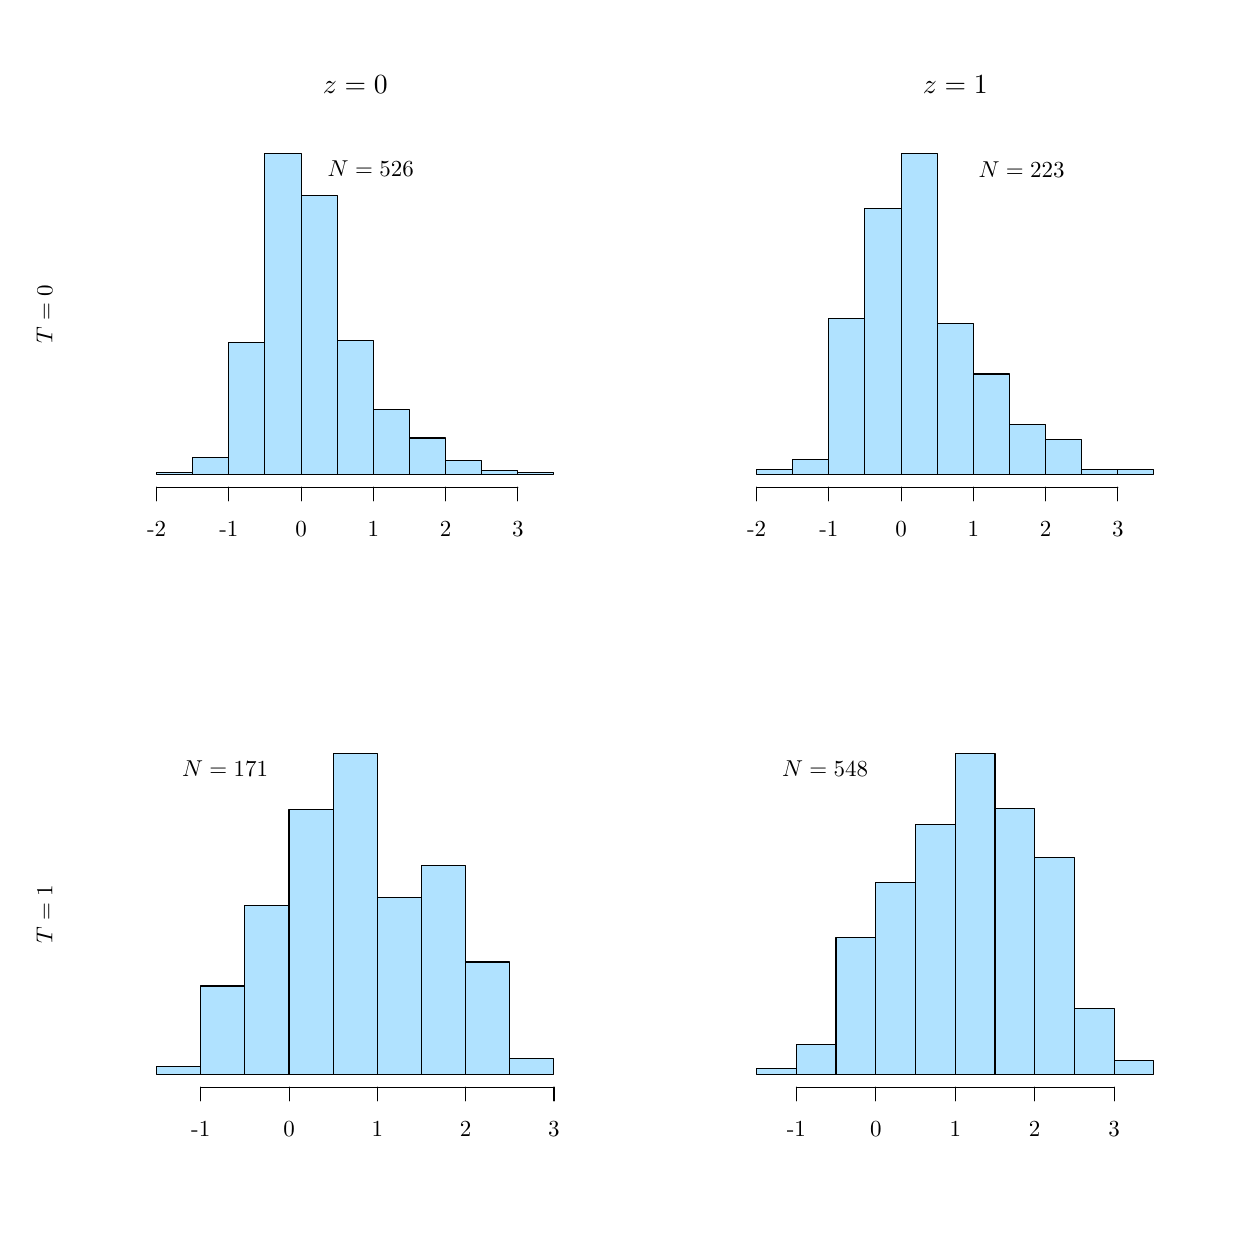
\begin{tikzpicture}[x=1pt,y=1pt]
\definecolor{fillColor}{RGB}{255,255,255}
\path[use as bounding box,fill=fillColor,fill opacity=0.00] (0,0) rectangle (433.62,433.62);
\begin{scope}
\path[clip] (  0.00,  0.00) rectangle (433.62,433.62);
\definecolor{drawColor}{RGB}{0,0,0}

\path[draw=drawColor,line width= 0.4pt,line join=round,line cap=round] ( 46.59,267.61) -- (177.11,267.61);

\path[draw=drawColor,line width= 0.4pt,line join=round,line cap=round] ( 46.59,267.61) -- ( 46.59,262.63);

\path[draw=drawColor,line width= 0.4pt,line join=round,line cap=round] ( 72.70,267.61) -- ( 72.70,262.63);

\path[draw=drawColor,line width= 0.4pt,line join=round,line cap=round] ( 98.80,267.61) -- ( 98.80,262.63);

\path[draw=drawColor,line width= 0.4pt,line join=round,line cap=round] (124.90,267.61) -- (124.90,262.63);

\path[draw=drawColor,line width= 0.4pt,line join=round,line cap=round] (151.01,267.61) -- (151.01,262.63);

\path[draw=drawColor,line width= 0.4pt,line join=round,line cap=round] (177.11,267.61) -- (177.11,262.63);

\node[text=drawColor,anchor=base,inner sep=0pt, outer sep=0pt, scale=  0.83] at ( 46.59,249.68) {-2};

\node[text=drawColor,anchor=base,inner sep=0pt, outer sep=0pt, scale=  0.83] at ( 72.70,249.68) {-1};

\node[text=drawColor,anchor=base,inner sep=0pt, outer sep=0pt, scale=  0.83] at ( 98.80,249.68) {0};

\node[text=drawColor,anchor=base,inner sep=0pt, outer sep=0pt, scale=  0.83] at (124.90,249.68) {1};

\node[text=drawColor,anchor=base,inner sep=0pt, outer sep=0pt, scale=  0.83] at (151.01,249.68) {2};

\node[text=drawColor,anchor=base,inner sep=0pt, outer sep=0pt, scale=  0.83] at (177.11,249.68) {3};
\end{scope}
\begin{scope}
\path[clip] (  0.00,216.81) rectangle (216.81,433.62);
\definecolor{drawColor}{RGB}{0,0,0}

\node[text=drawColor,anchor=base,inner sep=0pt, outer sep=0pt, scale=  1.00] at (118.36,409.77) {\bfseries $z = 0$};

\node[text=drawColor,rotate= 90.00,anchor=base,inner sep=0pt, outer sep=0pt, scale=  0.83] at (  8.96,330.19) {$T = 0$};
\end{scope}
\begin{scope}
\path[clip] ( 40.84,267.61) rectangle (195.89,392.78);
\definecolor{drawColor}{RGB}{0,0,0}
\definecolor{fillColor}{RGB}{176,226,255}

\path[draw=drawColor,line width= 0.4pt,line join=round,line cap=round,fill=fillColor] ( 46.58,272.24) rectangle ( 59.63,272.93);

\path[draw=drawColor,line width= 0.4pt,line join=round,line cap=round,fill=fillColor] ( 59.63,272.24) rectangle ( 72.68,278.45);

\path[draw=drawColor,line width= 0.4pt,line join=round,line cap=round,fill=fillColor] ( 72.68,272.24) rectangle ( 85.73,319.85);

\path[draw=drawColor,line width= 0.4pt,line join=round,line cap=round,fill=fillColor] ( 85.73,272.24) rectangle ( 98.79,388.15);

\path[draw=drawColor,line width= 0.4pt,line join=round,line cap=round,fill=fillColor] ( 98.79,272.24) rectangle (111.84,372.97);

\path[draw=drawColor,line width= 0.4pt,line join=round,line cap=round,fill=fillColor] (111.84,272.24) rectangle (124.89,320.54);

\path[draw=drawColor,line width= 0.4pt,line join=round,line cap=round,fill=fillColor] (124.89,272.24) rectangle (137.94,295.70);

\path[draw=drawColor,line width= 0.4pt,line join=round,line cap=round,fill=fillColor] (137.94,272.24) rectangle (151.00,285.35);

\path[draw=drawColor,line width= 0.4pt,line join=round,line cap=round,fill=fillColor] (151.00,272.24) rectangle (164.05,277.07);

\path[draw=drawColor,line width= 0.4pt,line join=round,line cap=round,fill=fillColor] (164.05,272.24) rectangle (177.10,273.62);

\path[draw=drawColor,line width= 0.4pt,line join=round,line cap=round,fill=fillColor] (177.10,272.24) rectangle (190.15,272.93);

\node[text=drawColor,anchor=base west,inner sep=0pt, outer sep=0pt, scale=  0.83] at (108.42,379.97) {$N=526$};
\end{scope}
\begin{scope}
\path[clip] (  0.00,  0.00) rectangle (433.62,433.62);
\definecolor{drawColor}{RGB}{0,0,0}

\path[draw=drawColor,line width= 0.4pt,line join=round,line cap=round] (263.40,267.61) -- (393.92,267.61);

\path[draw=drawColor,line width= 0.4pt,line join=round,line cap=round] (263.40,267.61) -- (263.40,262.63);

\path[draw=drawColor,line width= 0.4pt,line join=round,line cap=round] (289.51,267.61) -- (289.51,262.63);

\path[draw=drawColor,line width= 0.4pt,line join=round,line cap=round] (315.61,267.61) -- (315.61,262.63);

\path[draw=drawColor,line width= 0.4pt,line join=round,line cap=round] (341.71,267.61) -- (341.71,262.63);

\path[draw=drawColor,line width= 0.4pt,line join=round,line cap=round] (367.82,267.61) -- (367.82,262.63);

\path[draw=drawColor,line width= 0.4pt,line join=round,line cap=round] (393.92,267.61) -- (393.92,262.63);

\node[text=drawColor,anchor=base,inner sep=0pt, outer sep=0pt, scale=  0.83] at (263.40,249.68) {-2};

\node[text=drawColor,anchor=base,inner sep=0pt, outer sep=0pt, scale=  0.83] at (289.51,249.68) {-1};

\node[text=drawColor,anchor=base,inner sep=0pt, outer sep=0pt, scale=  0.83] at (315.61,249.68) {0};

\node[text=drawColor,anchor=base,inner sep=0pt, outer sep=0pt, scale=  0.83] at (341.71,249.68) {1};

\node[text=drawColor,anchor=base,inner sep=0pt, outer sep=0pt, scale=  0.83] at (367.82,249.68) {2};

\node[text=drawColor,anchor=base,inner sep=0pt, outer sep=0pt, scale=  0.83] at (393.92,249.68) {3};
\end{scope}
\begin{scope}
\path[clip] (216.81,216.81) rectangle (433.62,433.62);
\definecolor{drawColor}{RGB}{0,0,0}

\node[text=drawColor,anchor=base,inner sep=0pt, outer sep=0pt, scale=  1.00] at (335.17,409.77) {\bfseries $z = 1$};
\end{scope}
\begin{scope}
\path[clip] (257.65,267.61) rectangle (412.70,392.78);
\definecolor{drawColor}{RGB}{0,0,0}
\definecolor{fillColor}{RGB}{176,226,255}

\path[draw=drawColor,line width= 0.4pt,line join=round,line cap=round,fill=fillColor] (263.39,272.24) rectangle (276.44,274.05);

\path[draw=drawColor,line width= 0.4pt,line join=round,line cap=round,fill=fillColor] (276.44,272.24) rectangle (289.49,277.68);

\path[draw=drawColor,line width= 0.4pt,line join=round,line cap=round,fill=fillColor] (289.49,272.24) rectangle (302.54,328.38);

\path[draw=drawColor,line width= 0.4pt,line join=round,line cap=round,fill=fillColor] (302.54,272.24) rectangle (315.60,368.23);

\path[draw=drawColor,line width= 0.4pt,line join=round,line cap=round,fill=fillColor] (315.60,272.24) rectangle (328.65,388.15);

\path[draw=drawColor,line width= 0.4pt,line join=round,line cap=round,fill=fillColor] (328.65,272.24) rectangle (341.70,326.57);

\path[draw=drawColor,line width= 0.4pt,line join=round,line cap=round,fill=fillColor] (341.70,272.24) rectangle (354.75,308.46);

\path[draw=drawColor,line width= 0.4pt,line join=round,line cap=round,fill=fillColor] (354.75,272.24) rectangle (367.81,290.35);

\path[draw=drawColor,line width= 0.4pt,line join=round,line cap=round,fill=fillColor] (367.81,272.24) rectangle (380.86,284.92);

\path[draw=drawColor,line width= 0.4pt,line join=round,line cap=round,fill=fillColor] (380.86,272.24) rectangle (393.91,274.05);

\path[draw=drawColor,line width= 0.4pt,line join=round,line cap=round,fill=fillColor] (393.91,272.24) rectangle (406.96,274.05);

\node[text=drawColor,anchor=base west,inner sep=0pt, outer sep=0pt, scale=  0.83] at (343.60,379.49) {$N=223$};
\end{scope}
\begin{scope}
\path[clip] (  0.00,  0.00) rectangle (433.62,433.62);
\definecolor{drawColor}{RGB}{0,0,0}

\path[draw=drawColor,line width= 0.4pt,line join=round,line cap=round] ( 62.55, 50.80) -- (190.17, 50.80);

\path[draw=drawColor,line width= 0.4pt,line join=round,line cap=round] ( 62.55, 50.80) -- ( 62.55, 45.82);

\path[draw=drawColor,line width= 0.4pt,line join=round,line cap=round] ( 94.45, 50.80) -- ( 94.45, 45.82);

\path[draw=drawColor,line width= 0.4pt,line join=round,line cap=round] (126.36, 50.80) -- (126.36, 45.82);

\path[draw=drawColor,line width= 0.4pt,line join=round,line cap=round] (158.26, 50.80) -- (158.26, 45.82);

\path[draw=drawColor,line width= 0.4pt,line join=round,line cap=round] (190.17, 50.80) -- (190.17, 45.82);

\node[text=drawColor,anchor=base,inner sep=0pt, outer sep=0pt, scale=  0.83] at ( 62.55, 32.87) {-1};

\node[text=drawColor,anchor=base,inner sep=0pt, outer sep=0pt, scale=  0.83] at ( 94.45, 32.87) {0};

\node[text=drawColor,anchor=base,inner sep=0pt, outer sep=0pt, scale=  0.83] at (126.36, 32.87) {1};

\node[text=drawColor,anchor=base,inner sep=0pt, outer sep=0pt, scale=  0.83] at (158.26, 32.87) {2};

\node[text=drawColor,anchor=base,inner sep=0pt, outer sep=0pt, scale=  0.83] at (190.17, 32.87) {3};
\end{scope}
\begin{scope}
\path[clip] (  0.00,  0.00) rectangle (216.81,216.81);
\definecolor{drawColor}{RGB}{0,0,0}

\node[text=drawColor,rotate= 90.00,anchor=base,inner sep=0pt, outer sep=0pt, scale=  0.83] at (  8.96,113.38) {$T = 1$};
\end{scope}
\begin{scope}
\path[clip] ( 40.84, 50.80) rectangle (195.89,175.97);
\definecolor{drawColor}{RGB}{0,0,0}
\definecolor{fillColor}{RGB}{176,226,255}

\path[draw=drawColor,line width= 0.4pt,line join=round,line cap=round,fill=fillColor] ( 46.58, 55.43) rectangle ( 62.53, 58.33);

\path[draw=drawColor,line width= 0.4pt,line join=round,line cap=round,fill=fillColor] ( 62.53, 55.43) rectangle ( 78.48, 87.31);

\path[draw=drawColor,line width= 0.4pt,line join=round,line cap=round,fill=fillColor] ( 78.48, 55.43) rectangle ( 94.44,116.28);

\path[draw=drawColor,line width= 0.4pt,line join=round,line cap=round,fill=fillColor] ( 94.44, 55.43) rectangle (110.39,151.05);

\path[draw=drawColor,line width= 0.4pt,line join=round,line cap=round,fill=fillColor] (110.39, 55.43) rectangle (126.34,171.34);

\path[draw=drawColor,line width= 0.4pt,line join=round,line cap=round,fill=fillColor] (126.34, 55.43) rectangle (142.29,119.18);

\path[draw=drawColor,line width= 0.4pt,line join=round,line cap=round,fill=fillColor] (142.29, 55.43) rectangle (158.25,130.77);

\path[draw=drawColor,line width= 0.4pt,line join=round,line cap=round,fill=fillColor] (158.25, 55.43) rectangle (174.20, 96.00);

\path[draw=drawColor,line width= 0.4pt,line join=round,line cap=round,fill=fillColor] (174.20, 55.43) rectangle (190.15, 61.23);

\node[text=drawColor,anchor=base west,inner sep=0pt, outer sep=0pt, scale=  0.83] at ( 55.78,163.16) {$N=171$};
\end{scope}
\begin{scope}
\path[clip] (  0.00,  0.00) rectangle (433.62,433.62);
\definecolor{drawColor}{RGB}{0,0,0}

\path[draw=drawColor,line width= 0.4pt,line join=round,line cap=round] (277.76, 50.80) -- (392.62, 50.80);

\path[draw=drawColor,line width= 0.4pt,line join=round,line cap=round] (277.76, 50.80) -- (277.76, 45.82);

\path[draw=drawColor,line width= 0.4pt,line join=round,line cap=round] (306.47, 50.80) -- (306.47, 45.82);

\path[draw=drawColor,line width= 0.4pt,line join=round,line cap=round] (335.19, 50.80) -- (335.19, 45.82);

\path[draw=drawColor,line width= 0.4pt,line join=round,line cap=round] (363.90, 50.80) -- (363.90, 45.82);

\path[draw=drawColor,line width= 0.4pt,line join=round,line cap=round] (392.62, 50.80) -- (392.62, 45.82);

\node[text=drawColor,anchor=base,inner sep=0pt, outer sep=0pt, scale=  0.83] at (277.76, 32.87) {-1};

\node[text=drawColor,anchor=base,inner sep=0pt, outer sep=0pt, scale=  0.83] at (306.47, 32.87) {0};

\node[text=drawColor,anchor=base,inner sep=0pt, outer sep=0pt, scale=  0.83] at (335.19, 32.87) {1};

\node[text=drawColor,anchor=base,inner sep=0pt, outer sep=0pt, scale=  0.83] at (363.90, 32.87) {2};

\node[text=drawColor,anchor=base,inner sep=0pt, outer sep=0pt, scale=  0.83] at (392.62, 32.87) {3};
\end{scope}
\begin{scope}
\path[clip] (257.65, 50.80) rectangle (412.70,175.97);
\definecolor{drawColor}{RGB}{0,0,0}
\definecolor{fillColor}{RGB}{176,226,255}

\path[draw=drawColor,line width= 0.4pt,line join=round,line cap=round,fill=fillColor] (263.39, 55.43) rectangle (277.75, 57.41);

\path[draw=drawColor,line width= 0.4pt,line join=round,line cap=round,fill=fillColor] (277.75, 55.43) rectangle (292.10, 66.33);

\path[draw=drawColor,line width= 0.4pt,line join=round,line cap=round,fill=fillColor] (292.10, 55.43) rectangle (306.46,104.96);

\path[draw=drawColor,line width= 0.4pt,line join=round,line cap=round,fill=fillColor] (306.46, 55.43) rectangle (320.82,124.78);

\path[draw=drawColor,line width= 0.4pt,line join=round,line cap=round,fill=fillColor] (320.82, 55.43) rectangle (335.17,145.58);

\path[draw=drawColor,line width= 0.4pt,line join=round,line cap=round,fill=fillColor] (335.17, 55.43) rectangle (349.53,171.34);

\path[draw=drawColor,line width= 0.4pt,line join=round,line cap=round,fill=fillColor] (349.53, 55.43) rectangle (363.89,151.52);

\path[draw=drawColor,line width= 0.4pt,line join=round,line cap=round,fill=fillColor] (363.89, 55.43) rectangle (378.25,133.69);

\path[draw=drawColor,line width= 0.4pt,line join=round,line cap=round,fill=fillColor] (378.25, 55.43) rectangle (392.60, 79.21);

\path[draw=drawColor,line width= 0.4pt,line join=round,line cap=round,fill=fillColor] (392.60, 55.43) rectangle (406.96, 60.39);

\node[text=drawColor,anchor=base west,inner sep=0pt, outer sep=0pt, scale=  0.83] at (272.59,163.16) {$N=548$};
\end{scope}
\end{tikzpicture}

  \endgroup
\end{figure}
\end{frame}
%%%%%%%%%%%%%%%%%%%%%%%%%%%%%%%%%%%%%%%
\begin{frame}
  \frametitle{Empirical Illustration: Schooling and Test Scores}
\framesubtitle{Burde \& Linden (2013, AEJ Applied)}
    \begin{columns}[c]
    \column{.26\textwidth} 
    $\widehat{\beta}_{OLS} = 0.88$

    $\widehat{\beta}_{IV} = 1.27$

    $\widehat{\alpha}_1 - \widehat{\alpha}_0 = 0.18$
    \column{.73\textwidth}
        \begin{figure}[h]
          \scriptsize
          \begingroup
          \tikzset{every picture/.style={scale=0.53}}
          \centering
          % Created by tikzDevice version 0.8.1 on 2015-11-17 20:19:21
% !TEX encoding = UTF-8 Unicode
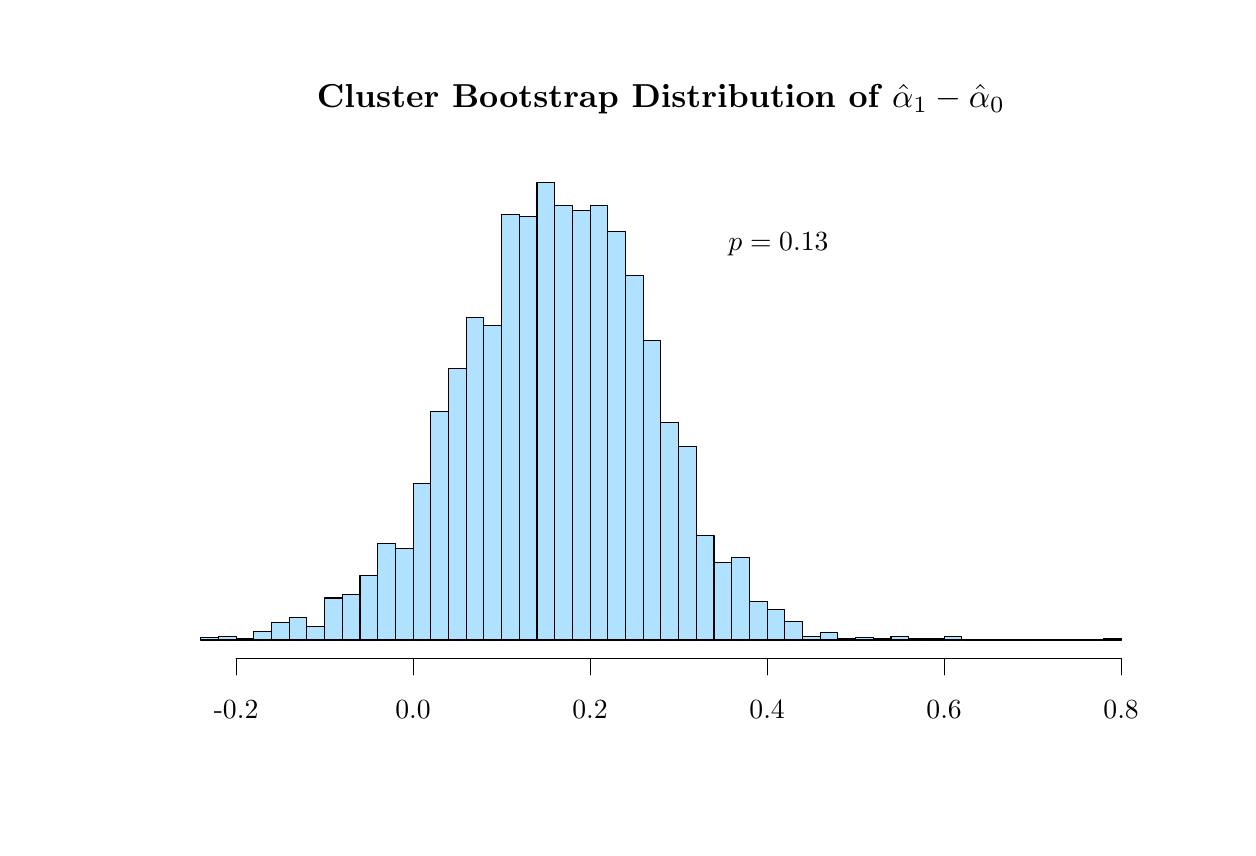
\begin{tikzpicture}[x=1pt,y=1pt]
\definecolor{fillColor}{RGB}{255,255,255}
\path[use as bounding box,fill=fillColor,fill opacity=0.00] (0,0) rectangle (433.62,289.08);
\begin{scope}
\path[clip] (  0.00,  0.00) rectangle (433.62,289.08);
\definecolor{drawColor}{RGB}{0,0,0}

\path[draw=drawColor,line width= 0.4pt,line join=round,line cap=round] ( 75.30, 61.20) -- (395.12, 61.20);

\path[draw=drawColor,line width= 0.4pt,line join=round,line cap=round] ( 75.30, 61.20) -- ( 75.30, 55.20);

\path[draw=drawColor,line width= 0.4pt,line join=round,line cap=round] (139.27, 61.20) -- (139.27, 55.20);

\path[draw=drawColor,line width= 0.4pt,line join=round,line cap=round] (203.23, 61.20) -- (203.23, 55.20);

\path[draw=drawColor,line width= 0.4pt,line join=round,line cap=round] (267.19, 61.20) -- (267.19, 55.20);

\path[draw=drawColor,line width= 0.4pt,line join=round,line cap=round] (331.16, 61.20) -- (331.16, 55.20);

\path[draw=drawColor,line width= 0.4pt,line join=round,line cap=round] (395.12, 61.20) -- (395.12, 55.20);

\node[text=drawColor,anchor=base,inner sep=0pt, outer sep=0pt, scale=  1.00] at ( 75.30, 39.60) {-0.2};

\node[text=drawColor,anchor=base,inner sep=0pt, outer sep=0pt, scale=  1.00] at (139.27, 39.60) {0.0};

\node[text=drawColor,anchor=base,inner sep=0pt, outer sep=0pt, scale=  1.00] at (203.23, 39.60) {0.2};

\node[text=drawColor,anchor=base,inner sep=0pt, outer sep=0pt, scale=  1.00] at (267.19, 39.60) {0.4};

\node[text=drawColor,anchor=base,inner sep=0pt, outer sep=0pt, scale=  1.00] at (331.16, 39.60) {0.6};

\node[text=drawColor,anchor=base,inner sep=0pt, outer sep=0pt, scale=  1.00] at (395.12, 39.60) {0.8};
\end{scope}
\begin{scope}
\path[clip] (  0.00,  0.00) rectangle (433.62,289.08);
\definecolor{drawColor}{RGB}{0,0,0}

\node[text=drawColor,anchor=base,inner sep=0pt, outer sep=0pt, scale=  1.20] at (228.81,260.34) {\bfseries Cluster Bootstrap Distribution of $\hat{\alpha}_1 - \hat{\alpha}_0$};
\end{scope}
\begin{scope}
\path[clip] ( 49.20, 61.20) rectangle (408.42,239.88);
\definecolor{drawColor}{RGB}{0,0,0}
\definecolor{fillColor}{RGB}{176,226,255}

\path[draw=drawColor,line width= 0.4pt,line join=round,line cap=round,fill=fillColor] ( 62.50, 67.82) rectangle ( 68.90, 68.71);

\path[draw=drawColor,line width= 0.4pt,line join=round,line cap=round,fill=fillColor] ( 68.90, 67.82) rectangle ( 75.30, 69.16);

\path[draw=drawColor,line width= 0.4pt,line join=round,line cap=round,fill=fillColor] ( 75.30, 67.82) rectangle ( 81.69, 68.26);

\path[draw=drawColor,line width= 0.4pt,line join=round,line cap=round,fill=fillColor] ( 81.69, 67.82) rectangle ( 88.09, 70.94);

\path[draw=drawColor,line width= 0.4pt,line join=round,line cap=round,fill=fillColor] ( 88.09, 67.82) rectangle ( 94.49, 74.06);

\path[draw=drawColor,line width= 0.4pt,line join=round,line cap=round,fill=fillColor] ( 94.49, 67.82) rectangle (100.88, 75.84);

\path[draw=drawColor,line width= 0.4pt,line join=round,line cap=round,fill=fillColor] (100.88, 67.82) rectangle (107.28, 72.72);

\path[draw=drawColor,line width= 0.4pt,line join=round,line cap=round,fill=fillColor] (107.28, 67.82) rectangle (113.68, 82.98);

\path[draw=drawColor,line width= 0.4pt,line join=round,line cap=round,fill=fillColor] (113.68, 67.82) rectangle (120.07, 84.32);

\path[draw=drawColor,line width= 0.4pt,line join=round,line cap=round,fill=fillColor] (120.07, 67.82) rectangle (126.47, 91.01);

\path[draw=drawColor,line width= 0.4pt,line join=round,line cap=round,fill=fillColor] (126.47, 67.82) rectangle (132.86,102.60);

\path[draw=drawColor,line width= 0.4pt,line join=round,line cap=round,fill=fillColor] (132.86, 67.82) rectangle (139.26,100.82);

\path[draw=drawColor,line width= 0.4pt,line join=round,line cap=round,fill=fillColor] (139.26, 67.82) rectangle (145.66,124.45);

\path[draw=drawColor,line width= 0.4pt,line join=round,line cap=round,fill=fillColor] (145.66, 67.82) rectangle (152.05,150.32);

\path[draw=drawColor,line width= 0.4pt,line join=round,line cap=round,fill=fillColor] (152.05, 67.82) rectangle (158.45,165.92);

\path[draw=drawColor,line width= 0.4pt,line join=round,line cap=round,fill=fillColor] (158.45, 67.82) rectangle (164.85,184.21);

\path[draw=drawColor,line width= 0.4pt,line join=round,line cap=round,fill=fillColor] (164.85, 67.82) rectangle (171.24,181.53);

\path[draw=drawColor,line width= 0.4pt,line join=round,line cap=round,fill=fillColor] (171.24, 67.82) rectangle (177.64,221.67);

\path[draw=drawColor,line width= 0.4pt,line join=round,line cap=round,fill=fillColor] (177.64, 67.82) rectangle (184.04,220.78);

\path[draw=drawColor,line width= 0.4pt,line join=round,line cap=round,fill=fillColor] (184.04, 67.82) rectangle (190.43,233.26);

\path[draw=drawColor,line width= 0.4pt,line join=round,line cap=round,fill=fillColor] (190.43, 67.82) rectangle (196.83,224.79);

\path[draw=drawColor,line width= 0.4pt,line join=round,line cap=round,fill=fillColor] (196.83, 67.82) rectangle (203.22,223.01);

\path[draw=drawColor,line width= 0.4pt,line join=round,line cap=round,fill=fillColor] (203.22, 67.82) rectangle (209.62,224.79);

\path[draw=drawColor,line width= 0.4pt,line join=round,line cap=round,fill=fillColor] (209.62, 67.82) rectangle (216.02,215.42);

\path[draw=drawColor,line width= 0.4pt,line join=round,line cap=round,fill=fillColor] (216.02, 67.82) rectangle (222.41,199.37);

\path[draw=drawColor,line width= 0.4pt,line join=round,line cap=round,fill=fillColor] (222.41, 67.82) rectangle (228.81,176.18);

\path[draw=drawColor,line width= 0.4pt,line join=round,line cap=round,fill=fillColor] (228.81, 67.82) rectangle (235.21,146.30);

\path[draw=drawColor,line width= 0.4pt,line join=round,line cap=round,fill=fillColor] (235.21, 67.82) rectangle (241.60,137.83);

\path[draw=drawColor,line width= 0.4pt,line join=round,line cap=round,fill=fillColor] (241.60, 67.82) rectangle (248.00,105.72);

\path[draw=drawColor,line width= 0.4pt,line join=round,line cap=round,fill=fillColor] (248.00, 67.82) rectangle (254.40, 95.91);

\path[draw=drawColor,line width= 0.4pt,line join=round,line cap=round,fill=fillColor] (254.40, 67.82) rectangle (260.79, 97.70);

\path[draw=drawColor,line width= 0.4pt,line join=round,line cap=round,fill=fillColor] (260.79, 67.82) rectangle (267.19, 81.64);

\path[draw=drawColor,line width= 0.4pt,line join=round,line cap=round,fill=fillColor] (267.19, 67.82) rectangle (273.58, 78.97);

\path[draw=drawColor,line width= 0.4pt,line join=round,line cap=round,fill=fillColor] (273.58, 67.82) rectangle (279.98, 74.51);

\path[draw=drawColor,line width= 0.4pt,line join=round,line cap=round,fill=fillColor] (279.98, 67.82) rectangle (286.38, 69.16);

\path[draw=drawColor,line width= 0.4pt,line join=round,line cap=round,fill=fillColor] (286.38, 67.82) rectangle (292.77, 70.49);

\path[draw=drawColor,line width= 0.4pt,line join=round,line cap=round,fill=fillColor] (292.77, 67.82) rectangle (299.17, 68.26);

\path[draw=drawColor,line width= 0.4pt,line join=round,line cap=round,fill=fillColor] (299.17, 67.82) rectangle (305.57, 68.71);

\path[draw=drawColor,line width= 0.4pt,line join=round,line cap=round,fill=fillColor] (305.57, 67.82) rectangle (311.96, 68.26);

\path[draw=drawColor,line width= 0.4pt,line join=round,line cap=round,fill=fillColor] (311.96, 67.82) rectangle (318.36, 69.16);

\path[draw=drawColor,line width= 0.4pt,line join=round,line cap=round,fill=fillColor] (318.36, 67.82) rectangle (324.76, 68.26);

\path[draw=drawColor,line width= 0.4pt,line join=round,line cap=round,fill=fillColor] (324.76, 67.82) rectangle (331.15, 68.26);

\path[draw=drawColor,line width= 0.4pt,line join=round,line cap=round,fill=fillColor] (331.15, 67.82) rectangle (337.55, 69.16);

\path[draw=drawColor,line width= 0.4pt,line join=round,line cap=round,fill=fillColor] (337.55, 67.82) rectangle (343.94, 67.82);

\path[draw=drawColor,line width= 0.4pt,line join=round,line cap=round,fill=fillColor] (343.94, 67.82) rectangle (350.34, 67.82);

\path[draw=drawColor,line width= 0.4pt,line join=round,line cap=round,fill=fillColor] (350.34, 67.82) rectangle (356.74, 67.82);

\path[draw=drawColor,line width= 0.4pt,line join=round,line cap=round,fill=fillColor] (356.74, 67.82) rectangle (363.13, 67.82);

\path[draw=drawColor,line width= 0.4pt,line join=round,line cap=round,fill=fillColor] (363.13, 67.82) rectangle (369.53, 67.82);

\path[draw=drawColor,line width= 0.4pt,line join=round,line cap=round,fill=fillColor] (369.53, 67.82) rectangle (375.93, 67.82);

\path[draw=drawColor,line width= 0.4pt,line join=round,line cap=round,fill=fillColor] (375.93, 67.82) rectangle (382.32, 67.82);

\path[draw=drawColor,line width= 0.4pt,line join=round,line cap=round,fill=fillColor] (382.32, 67.82) rectangle (388.72, 67.82);

\path[draw=drawColor,line width= 0.4pt,line join=round,line cap=round,fill=fillColor] (388.72, 67.82) rectangle (395.12, 68.26);

\node[text=drawColor,anchor=base west,inner sep=0pt, outer sep=0pt, scale=  1.00] at (253.21,208.45) {$p = 0.13$};
\end{scope}
\end{tikzpicture}

          \endgroup
        \end{figure}
    \end{columns}
\end{frame}

%%%%%%%%%%%%%%%%%%%%%%%%%%%%%%%%%%%%%%
\begin{frame}
  \begin{center}
    \huge But what if $z$ is endogenous? \\
  \end{center}
\end{frame}
%%%%%%%%%%%%%%%%%%%%%%%%%%%%%%%%%%%%%%
\begin{frame}

  \begin{block}{Recall: Unrestricted System}
    \vspace{-1.5em}
    \small
  \begin{eqnarray*}
   \widetilde{y}_{0k}&=&  (\beta + m_{1k}^*) \alpha_1 p_k^*  + (1 -\alpha_0)(1 - p^*_k)m_{0k}^*  \\  
   \widetilde{y}_{1k}&=& (\beta + m_{1k}^*) (1 - \alpha_1)p_k^* + \alpha_0 (1 - p_k^*) m_{0k}^*
  \end{eqnarray*}
  \end{block}

  \begin{alertblock}{Intelligible Quantities}
    \vspace{-1.5em}
    \begin{eqnarray*}
      \delta_{T^*} &\equiv& \mathbb{E}\left[ u|T^*=1 \right] - \mathbb{E}\left[u|T^*=0 \right] \\
      \delta_{z} &\equiv& \mathbb{E}\left[ u|z=1 \right] - \mathbb{E}\left[u|z=0 \right] 
    \end{eqnarray*}
   \hfill \alert{\ldots both are linear functions of $m_{tk}^*$.}
  \end{alertblock}

\end{frame}
%%%%%%%%%%%%%%%%%%%%%%%%%%%%%%%%%%%%%%
\begin{frame}
  \begin{block}{First Moment Information}
  \frametitle{Identified Set for $(\alpha_0, \alpha_1, \delta_{T^*}, \delta_z)$}
  \[
    \delta_z = C(\alpha_0, \alpha_1|\mathbf{p}, \mathbf{q}, \mathbf{\bar{y}}) - \left( \frac{p_1 - p_2}{1 - \alpha_0 - \alpha_1} \right) \delta_{T^*}
  \]
  \end{block}
  \begin{block}{Second Moment Information}
    \[Var(u|T = t,z = k) > 0\]  \[\implies
      \left[Var(y|T=t, z=k) - Q_{tk}(\delta_{T^*}, \delta_z,\alpha_0, \alpha_1|\mathbf{p}, \mathbf{q}, \mathbf{\bar{y}})\right] > 0\]

  \end{block}
\end{frame}
%%%%%%%%%%%%%%%%%%%%%%%%%%%%%%%%%%%%%%
\begin{frame}
  \frametitle{Approaches to (Partial) Identification}
  \begin{block}{Identification}
    \begin{itemize}
      \item $\delta_z = 0, \alpha_0 = \alpha_1 = 0 \Rightarrow$ Wald Estimator
    \item Joint Exogeneity ($\Rightarrow \delta_{T^*} = \delta_z = 0$)\\
      \footnotesize Kane et al. (1999), Black et al.\ (2000), Mahajan (2006)\ldots
    \end{itemize}
    
  \end{block}

  \begin{block}{Partial Identification}
    \begin{itemize}
      \item Frazis \& Loewenstein (2003): $\delta_z = 0$, $(\alpha_0 + \alpha_1) \in [\ell, u]$ 
    \item Conley et al.\ (2012): $\delta_z \in [\underline{\delta}_z, \bar{\delta}_z]$, $\alpha_0 = \alpha_1 = 0$
    \item Nevo \& Rosen (2012): $\delta_T^* > \delta_z$, $\delta_T^* \delta_z > 0$, $\alpha_0 = \alpha_1 = 0$
    \end{itemize}
  \end{block}
    
\end{frame}
%%%%%%%%%%%%%%%%%%%%%%%%%%%%%%%%%%%%%%%
\begin{frame}
  \frametitle{Our Proposed Approach}
  \begin{block}{Elicit Beliefs}
    Ask researcher for bounds on $\alpha_0, \alpha_1, \delta_{T^*}, \delta_z$ 
  \end{block}

  \begin{block}{Discipline Beliefs}
    Are these beliefs mutually consistent? Explore joint constraints implied by identified set.
    
  \end{block}
  \begin{block}{Incorporate Beliefs}
    Carry out (Bayesian) inference for $\beta$ using beliefs, constraints, and accounting for sampling uncertainty.
  \end{block}
\end{frame}
%%%%%%%%%%%%%%%%%%%%%%%%%%%%%%%%%%%%%%%
\begin{frame}
  \frametitle{Example: Vouchers for Private Schooling (PACES)}
  \framesubtitle{Angrist et al.\ (2002, AER)}

  Data from Colombia: vouchers to attend private school awarded by lottery to poor, primary school-aged children (N = 1577). 
  

\begin{itemize}
  \item $y$ -- \# of grades repeated after lottery
  \item $T^*$ -- Scholarship use 
  \item $T$ -- Self-reported Scholarship use
  \item $\mathbf{x}$ -- Demographic controls
  \item $z$ -- Offered scholarship through lottery 
\end{itemize}

\alert{Authors raise concerns about the lottery in one of the two cities\ldots}
\end{frame}

%%%%%%%%%%%%%%%%%%%%%%%%%%%%%%%%%%%%%%%
\begin{frame}
  \frametitle{Example: Vouchers for Private Schooling (PACES)}
  \framesubtitle{Overall: Mean = 0.19, SD = 0.45}
\begin{figure}[h]
  \scriptsize
  \begingroup
  \tikzset{every picture/.style={scale=0.53}}
  \centering
  \input{../../../sick-instruments/fig/AngristBettinger/hist.tex}
  \endgroup
\end{figure}
\end{frame}
%%%%%%%%%%%%%%%%%%%%%%%%%%%%%%%%%%%%%%%
\begin{frame}
  \frametitle{Implications of Valid IV: $\delta_z = 0$}
  \framesubtitle{Angrist et al.\ (2002)}
\begin{figure}[h]
  \scriptsize
  \begingroup
  \tikzset{every picture/.style={scale=0.33}}
  \centering
  \input{../../../sick-instruments/fig/AngristBettinger/validIV.tex}
  \endgroup
\end{figure}
\end{frame}
%%%%%%%%%%%%%%%%%%%%%%%%%%%%%%%%%%%%%%%
\begin{frame}
  \frametitle{Implications of Negative Selection: $\delta_{T^*} = -0.75$}
\begin{figure}[h]
  \scriptsize
  \begingroup
  \tikzset{every picture/.style={scale=0.53}}
  \centering
  \input{../../../sick-instruments/fig/AngristBettinger/dTstar_neg75.tex}
  \endgroup
\end{figure}
\end{frame}
%%%%%%%%%%%%%%%%%%%%%%%%%%%%%%%%%%%%%%%
\begin{frame}
  \frametitle{Implications of Negative Selection: $\delta_{T^*} = -0.60$}
\begin{figure}[h]
  \scriptsize
  \begingroup
  \tikzset{every picture/.style={scale=0.53}}
  \centering
  \input{../../../sick-instruments/fig/AngristBettinger/dTstar_neg60.tex}
  \endgroup
\end{figure}
\end{frame}
%%%%%%%%%%%%%%%%%%%%%%%%%%%%%%%%%%%%%%%
\begin{frame}
  \frametitle{Conclusion}
  \begin{itemize}
    \item Effect of endogenous, mis-measured, binary treatment.
    \item Important in applied work but no solution in the literature.
    \item New partial and point identification results by exploiting higher moments of outcome variable.
    \item Test necessary condition for absence of measurement error.
    %\item Explore sampling distribution of our simple closed-form method of moments estimator in a simulation experiment.
    %\item Detect evidence of measurement error in real-world example. 
    \item Next steps: use full independence of $z \rightarrow$ optimal estimator
  \end{itemize}
\end{frame}
%%%%%%%%%%%%%%%%%%%%%%%%%%%%%%%%%%%%%%
\appendix
%%%%%%%%%%%%%%%%%%%%%%%%%%%%%%%%%%%%%
\begin{frame}
  \begin{center}
    \Huge Simulation Study
  \end{center}
\end{frame}
%%%%%%%%%%%%%%%%%%%%%%%%%%%%%%%%%%%%%
\begin{frame}
  \frametitle{Simulation Study: $y = \beta T^* + \varepsilon$}
  \begin{itemize}
    \item $(\varepsilon, \eta) \sim $ jointly normal, mean 0, variance 1, corr.\ 0.3.
    \item First stage: $T^* = \mathbf{1}\left\{ \gamma_0 + \gamma_1 z + \eta > 0 \right\}$
      \begin{itemize}
        \item Half of subjects have $z=1$, the rest have $z=0$.
        \item $\gamma_0 = \Phi^{-1}(\delta)$
        \item $\gamma_1 = \Phi^{-1}(1-\delta) - \Phi(\delta)$   
        \item $\delta$ equals fraction of those offered treatment who fail to take it up \emph{and} fraction of those not offered treatment who do.
      \end{itemize}
    \item Generate $T$ as follows:
      \begin{itemize}
        \item $T^* = 0 \implies T=0$, i.e.\ $\alpha_0 = 0$
        \item $T|T^*=1 \sim \mbox{Bernoulli}(1-\alpha_1)$
        \item $\alpha_0, \alpha_1$ unknown to econometrician.
      \end{itemize}
  \end{itemize}

  
\end{frame}
%%%%%%%%%%%%%%%%%%%%%%%%%%%%%%%%%%%%%%
\begin{frame}
  \begin{center}
    {\framebox{\Large Sampling Distribution of $\widehat{\alpha}_1 - \widehat{\alpha}_0$}}
  \end{center}
\end{frame}
%%%%%%%%%%%%%%%%%%%%%%%%%%%%%%%%%%%%%%
%\begin{frame}
%\begin{figure}[h]
%  \scriptsize
%  \begingroup
%  \tikzset{every picture/.style={scale=0.53}}
%  \centering
%  \begin{subfigure}[b]{0.31\textwidth}
%\caption{\footnotesize $N=500, \delta = 0.1$}
%  % Created by tikzDevice version 0.8.1 on 2015-11-17 12:44:46
% !TEX encoding = UTF-8 Unicode
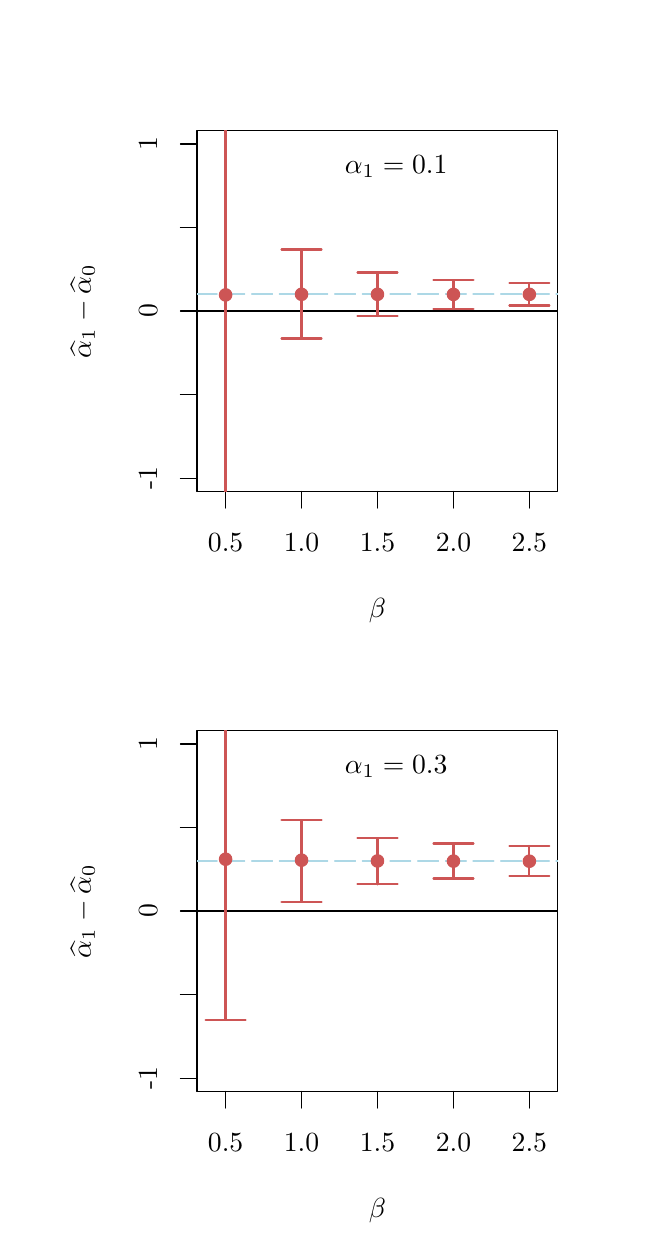
\begin{tikzpicture}[x=1pt,y=1pt]
\definecolor{fillColor}{RGB}{255,255,255}
\path[use as bounding box,fill=fillColor,fill opacity=0.00] (0,0) rectangle (216.81,433.62);
\begin{scope}
\path[clip] (  0.00,  0.00) rectangle (216.81,433.62);
\definecolor{drawColor}{RGB}{0,0,0}

\path[draw=drawColor,line width= 0.4pt,line join=round,line cap=round] ( 71.52,266.01) -- (181.29,266.01);

\path[draw=drawColor,line width= 0.4pt,line join=round,line cap=round] ( 71.52,266.01) -- ( 71.52,260.01);

\path[draw=drawColor,line width= 0.4pt,line join=round,line cap=round] ( 98.96,266.01) -- ( 98.96,260.01);

\path[draw=drawColor,line width= 0.4pt,line join=round,line cap=round] (126.40,266.01) -- (126.40,260.01);

\path[draw=drawColor,line width= 0.4pt,line join=round,line cap=round] (153.85,266.01) -- (153.85,260.01);

\path[draw=drawColor,line width= 0.4pt,line join=round,line cap=round] (181.29,266.01) -- (181.29,260.01);

\node[text=drawColor,anchor=base,inner sep=0pt, outer sep=0pt, scale=  1.00] at ( 71.52,244.41) {0.5};

\node[text=drawColor,anchor=base,inner sep=0pt, outer sep=0pt, scale=  1.00] at ( 98.96,244.41) {1.0};

\node[text=drawColor,anchor=base,inner sep=0pt, outer sep=0pt, scale=  1.00] at (126.40,244.41) {1.5};

\node[text=drawColor,anchor=base,inner sep=0pt, outer sep=0pt, scale=  1.00] at (153.85,244.41) {2.0};

\node[text=drawColor,anchor=base,inner sep=0pt, outer sep=0pt, scale=  1.00] at (181.29,244.41) {2.5};

\path[draw=drawColor,line width= 0.4pt,line join=round,line cap=round] ( 61.20,266.01) --
	(191.61,266.01) --
	(191.61,396.42) --
	( 61.20,396.42) --
	( 61.20,266.01);
\end{scope}
\begin{scope}
\path[clip] (  0.00,216.81) rectangle (216.81,433.62);
\definecolor{drawColor}{RGB}{0,0,0}

\node[text=drawColor,anchor=base,inner sep=0pt, outer sep=0pt, scale=  1.00] at (126.41,220.41) {$\beta$};

\node[text=drawColor,rotate= 90.00,anchor=base,inner sep=0pt, outer sep=0pt, scale=  1.00] at ( 22.80,331.22) {$\widehat{\alpha}_1 - \widehat{\alpha}_0$};
\end{scope}
\begin{scope}
\path[clip] (  0.00,  0.00) rectangle (216.81,433.62);
\definecolor{drawColor}{RGB}{0,0,0}

\path[draw=drawColor,line width= 0.4pt,line join=round,line cap=round] ( 61.20,270.84) -- ( 61.20,391.59);

\path[draw=drawColor,line width= 0.4pt,line join=round,line cap=round] ( 61.20,270.84) -- ( 55.20,270.84);

\path[draw=drawColor,line width= 0.4pt,line join=round,line cap=round] ( 61.20,301.03) -- ( 55.20,301.03);

\path[draw=drawColor,line width= 0.4pt,line join=round,line cap=round] ( 61.20,331.22) -- ( 55.20,331.22);

\path[draw=drawColor,line width= 0.4pt,line join=round,line cap=round] ( 61.20,361.40) -- ( 55.20,361.40);

\path[draw=drawColor,line width= 0.4pt,line join=round,line cap=round] ( 61.20,391.59) -- ( 55.20,391.59);

\node[text=drawColor,rotate= 90.00,anchor=base,inner sep=0pt, outer sep=0pt, scale=  1.00] at ( 46.80,270.84) {-1};

\node[text=drawColor,rotate= 90.00,anchor=base,inner sep=0pt, outer sep=0pt, scale=  1.00] at ( 46.80,331.22) {0};

\node[text=drawColor,rotate= 90.00,anchor=base,inner sep=0pt, outer sep=0pt, scale=  1.00] at ( 46.80,391.59) {1};
\end{scope}
\begin{scope}
\path[clip] ( 61.20,266.01) rectangle (191.61,396.42);
\definecolor{drawColor}{RGB}{0,0,0}

\node[text=drawColor,anchor=base west,inner sep=0pt, outer sep=0pt, scale=  1.00] at (114.66,380.98) {$\alpha_1=0.1$};
\definecolor{drawColor}{RGB}{173,216,230}

\path[draw=drawColor,line width= 0.8pt,dash pattern=on 7pt off 3pt ,line join=round,line cap=round] ( 61.20,337.25) -- (191.61,337.25);

\path[draw=drawColor,line width= 0.8pt,dash pattern=on 7pt off 3pt ,line join=round,line cap=round] ( 61.20,337.25) -- (191.61,337.25);

\path[draw=drawColor,line width= 0.8pt,dash pattern=on 7pt off 3pt ,line join=round,line cap=round] ( 61.20,337.25) -- (191.61,337.25);

\path[draw=drawColor,line width= 0.8pt,dash pattern=on 7pt off 3pt ,line join=round,line cap=round] ( 61.20,337.25) -- (191.61,337.25);

\path[draw=drawColor,line width= 0.8pt,dash pattern=on 7pt off 3pt ,line join=round,line cap=round] ( 61.20,337.25) -- (191.61,337.25);
\definecolor{drawColor}{RGB}{0,0,0}

\path[draw=drawColor,line width= 0.4pt,line join=round,line cap=round] ( 61.20,331.22) -- (191.61,331.22);
\definecolor{drawColor}{RGB}{205,85,85}

\path[draw=drawColor,line width= 0.8pt,line join=round,line cap=round] ( 71.52,263.63) -- ( 71.52,411.66);

\path[draw=drawColor,line width= 0.8pt,line join=round,line cap=round] ( 64.29,263.63) --
	( 71.52,263.63) --
	( 78.75,263.63);

\path[draw=drawColor,line width= 0.8pt,line join=round,line cap=round] ( 78.75,411.66) --
	( 71.52,411.66) --
	( 64.29,411.66);

\path[draw=drawColor,line width= 0.8pt,line join=round,line cap=round] ( 98.96,321.26) -- ( 98.96,353.42);

\path[draw=drawColor,line width= 0.8pt,line join=round,line cap=round] ( 91.73,321.26) --
	( 98.96,321.26) --
	(106.19,321.26);

\path[draw=drawColor,line width= 0.8pt,line join=round,line cap=round] (106.19,353.42) --
	( 98.96,353.42) --
	( 91.73,353.42);

\path[draw=drawColor,line width= 0.8pt,line join=round,line cap=round] (126.40,329.44) -- (126.40,345.11);

\path[draw=drawColor,line width= 0.8pt,line join=round,line cap=round] (119.18,329.44) --
	(126.40,329.44) --
	(133.63,329.44);

\path[draw=drawColor,line width= 0.8pt,line join=round,line cap=round] (133.63,345.11) --
	(126.40,345.11) --
	(119.18,345.11);

\path[draw=drawColor,line width= 0.8pt,line join=round,line cap=round] (153.85,332.05) -- (153.85,342.36);

\path[draw=drawColor,line width= 0.8pt,line join=round,line cap=round] (146.62,332.05) --
	(153.85,332.05) --
	(161.08,332.05);

\path[draw=drawColor,line width= 0.8pt,line join=round,line cap=round] (161.08,342.36) --
	(153.85,342.36) --
	(146.62,342.36);

\path[draw=drawColor,line width= 0.8pt,line join=round,line cap=round] (181.29,333.23) -- (181.29,341.24);

\path[draw=drawColor,line width= 0.8pt,line join=round,line cap=round] (174.06,333.23) --
	(181.29,333.23) --
	(188.52,333.23);

\path[draw=drawColor,line width= 0.8pt,line join=round,line cap=round] (188.52,341.24) --
	(181.29,341.24) --
	(174.06,341.24);
\definecolor{fillColor}{RGB}{205,85,85}

\path[draw=drawColor,line width= 0.4pt,line join=round,line cap=round,fill=fillColor] ( 71.52,337.05) circle (  2.25);

\path[draw=drawColor,line width= 0.4pt,line join=round,line cap=round,fill=fillColor] ( 98.96,337.27) circle (  2.25);

\path[draw=drawColor,line width= 0.4pt,line join=round,line cap=round,fill=fillColor] (126.40,337.26) circle (  2.25);

\path[draw=drawColor,line width= 0.4pt,line join=round,line cap=round,fill=fillColor] (153.85,337.23) circle (  2.25);

\path[draw=drawColor,line width= 0.4pt,line join=round,line cap=round,fill=fillColor] (181.29,337.25) circle (  2.25);
\end{scope}
\begin{scope}
\path[clip] (  0.00,  0.00) rectangle (216.81,433.62);
\definecolor{drawColor}{RGB}{0,0,0}

\path[draw=drawColor,line width= 0.4pt,line join=round,line cap=round] ( 71.52, 49.20) -- (181.29, 49.20);

\path[draw=drawColor,line width= 0.4pt,line join=round,line cap=round] ( 71.52, 49.20) -- ( 71.52, 43.20);

\path[draw=drawColor,line width= 0.4pt,line join=round,line cap=round] ( 98.96, 49.20) -- ( 98.96, 43.20);

\path[draw=drawColor,line width= 0.4pt,line join=round,line cap=round] (126.40, 49.20) -- (126.40, 43.20);

\path[draw=drawColor,line width= 0.4pt,line join=round,line cap=round] (153.85, 49.20) -- (153.85, 43.20);

\path[draw=drawColor,line width= 0.4pt,line join=round,line cap=round] (181.29, 49.20) -- (181.29, 43.20);

\node[text=drawColor,anchor=base,inner sep=0pt, outer sep=0pt, scale=  1.00] at ( 71.52, 27.60) {0.5};

\node[text=drawColor,anchor=base,inner sep=0pt, outer sep=0pt, scale=  1.00] at ( 98.96, 27.60) {1.0};

\node[text=drawColor,anchor=base,inner sep=0pt, outer sep=0pt, scale=  1.00] at (126.40, 27.60) {1.5};

\node[text=drawColor,anchor=base,inner sep=0pt, outer sep=0pt, scale=  1.00] at (153.85, 27.60) {2.0};

\node[text=drawColor,anchor=base,inner sep=0pt, outer sep=0pt, scale=  1.00] at (181.29, 27.60) {2.5};

\path[draw=drawColor,line width= 0.4pt,line join=round,line cap=round] ( 61.20, 49.20) --
	(191.61, 49.20) --
	(191.61,179.61) --
	( 61.20,179.61) --
	( 61.20, 49.20);
\end{scope}
\begin{scope}
\path[clip] (  0.00,  0.00) rectangle (216.81,216.81);
\definecolor{drawColor}{RGB}{0,0,0}

\node[text=drawColor,anchor=base,inner sep=0pt, outer sep=0pt, scale=  1.00] at (126.41,  3.60) {$\beta$};

\node[text=drawColor,rotate= 90.00,anchor=base,inner sep=0pt, outer sep=0pt, scale=  1.00] at ( 22.80,114.41) {$\widehat{\alpha}_1 - \widehat{\alpha}_0$};
\end{scope}
\begin{scope}
\path[clip] (  0.00,  0.00) rectangle (216.81,433.62);
\definecolor{drawColor}{RGB}{0,0,0}

\path[draw=drawColor,line width= 0.4pt,line join=round,line cap=round] ( 61.20, 54.03) -- ( 61.20,174.78);

\path[draw=drawColor,line width= 0.4pt,line join=round,line cap=round] ( 61.20, 54.03) -- ( 55.20, 54.03);

\path[draw=drawColor,line width= 0.4pt,line join=round,line cap=round] ( 61.20, 84.22) -- ( 55.20, 84.22);

\path[draw=drawColor,line width= 0.4pt,line join=round,line cap=round] ( 61.20,114.41) -- ( 55.20,114.41);

\path[draw=drawColor,line width= 0.4pt,line join=round,line cap=round] ( 61.20,144.59) -- ( 55.20,144.59);

\path[draw=drawColor,line width= 0.4pt,line join=round,line cap=round] ( 61.20,174.78) -- ( 55.20,174.78);

\node[text=drawColor,rotate= 90.00,anchor=base,inner sep=0pt, outer sep=0pt, scale=  1.00] at ( 46.80, 54.03) {-1};

\node[text=drawColor,rotate= 90.00,anchor=base,inner sep=0pt, outer sep=0pt, scale=  1.00] at ( 46.80,114.41) {0};

\node[text=drawColor,rotate= 90.00,anchor=base,inner sep=0pt, outer sep=0pt, scale=  1.00] at ( 46.80,174.78) {1};
\end{scope}
\begin{scope}
\path[clip] ( 61.20, 49.20) rectangle (191.61,179.61);
\definecolor{drawColor}{RGB}{0,0,0}

\node[text=drawColor,anchor=base west,inner sep=0pt, outer sep=0pt, scale=  1.00] at (114.66,164.17) {$\alpha_1=0.3$};
\definecolor{drawColor}{RGB}{173,216,230}

\path[draw=drawColor,line width= 0.8pt,dash pattern=on 7pt off 3pt ,line join=round,line cap=round] ( 61.20,132.52) -- (191.61,132.52);

\path[draw=drawColor,line width= 0.8pt,dash pattern=on 7pt off 3pt ,line join=round,line cap=round] ( 61.20,132.52) -- (191.61,132.52);

\path[draw=drawColor,line width= 0.8pt,dash pattern=on 7pt off 3pt ,line join=round,line cap=round] ( 61.20,132.52) -- (191.61,132.52);

\path[draw=drawColor,line width= 0.8pt,dash pattern=on 7pt off 3pt ,line join=round,line cap=round] ( 61.20,132.52) -- (191.61,132.52);

\path[draw=drawColor,line width= 0.8pt,dash pattern=on 7pt off 3pt ,line join=round,line cap=round] ( 61.20,132.52) -- (191.61,132.52);
\definecolor{drawColor}{RGB}{0,0,0}

\path[draw=drawColor,line width= 0.4pt,line join=round,line cap=round] ( 61.20,114.41) -- (191.61,114.41);
\definecolor{drawColor}{RGB}{205,85,85}

\path[draw=drawColor,line width= 0.8pt,line join=round,line cap=round] ( 71.52, 75.16) -- ( 71.52,193.94);

\path[draw=drawColor,line width= 0.8pt,line join=round,line cap=round] ( 64.29, 75.16) --
	( 71.52, 75.16) --
	( 78.75, 75.16);

\path[draw=drawColor,line width= 0.8pt,line join=round,line cap=round] ( 78.75,193.94) --
	( 71.52,193.94) --
	( 64.29,193.94);

\path[draw=drawColor,line width= 0.8pt,line join=round,line cap=round] ( 98.96,117.78) -- ( 98.96,147.23);

\path[draw=drawColor,line width= 0.8pt,line join=round,line cap=round] ( 91.73,117.78) --
	( 98.96,117.78) --
	(106.19,117.78);

\path[draw=drawColor,line width= 0.8pt,line join=round,line cap=round] (106.19,147.23) --
	( 98.96,147.23) --
	( 91.73,147.23);

\path[draw=drawColor,line width= 0.8pt,line join=round,line cap=round] (126.40,124.05) -- (126.40,140.70);

\path[draw=drawColor,line width= 0.8pt,line join=round,line cap=round] (119.18,124.05) --
	(126.40,124.05) --
	(133.63,124.05);

\path[draw=drawColor,line width= 0.8pt,line join=round,line cap=round] (133.63,140.70) --
	(126.40,140.70) --
	(119.18,140.70);

\path[draw=drawColor,line width= 0.8pt,line join=round,line cap=round] (153.85,126.18) -- (153.85,138.79);

\path[draw=drawColor,line width= 0.8pt,line join=round,line cap=round] (146.62,126.18) --
	(153.85,126.18) --
	(161.08,126.18);

\path[draw=drawColor,line width= 0.8pt,line join=round,line cap=round] (161.08,138.79) --
	(153.85,138.79) --
	(146.62,138.79);

\path[draw=drawColor,line width= 0.8pt,line join=round,line cap=round] (181.29,127.20) -- (181.29,137.88);

\path[draw=drawColor,line width= 0.8pt,line join=round,line cap=round] (174.06,127.20) --
	(181.29,127.20) --
	(188.52,127.20);

\path[draw=drawColor,line width= 0.8pt,line join=round,line cap=round] (188.52,137.88) --
	(181.29,137.88) --
	(174.06,137.88);
\definecolor{fillColor}{RGB}{205,85,85}

\path[draw=drawColor,line width= 0.4pt,line join=round,line cap=round,fill=fillColor] ( 71.52,133.14) circle (  2.25);

\path[draw=drawColor,line width= 0.4pt,line join=round,line cap=round,fill=fillColor] ( 98.96,132.79) circle (  2.25);

\path[draw=drawColor,line width= 0.4pt,line join=round,line cap=round,fill=fillColor] (126.40,132.51) circle (  2.25);

\path[draw=drawColor,line width= 0.4pt,line join=round,line cap=round,fill=fillColor] (153.85,132.45) circle (  2.25);

\path[draw=drawColor,line width= 0.4pt,line join=round,line cap=round,fill=fillColor] (181.29,132.42) circle (  2.25);
\end{scope}
\end{tikzpicture}

%  \end{subfigure}
%  ~
%  \begin{subfigure}[b]{0.31\textwidth}
%    \caption{\footnotesize $N=1000, \delta = 0.1$} 
%  % Created by tikzDevice version 0.8.1 on 2015-11-17 11:43:47
% !TEX encoding = UTF-8 Unicode
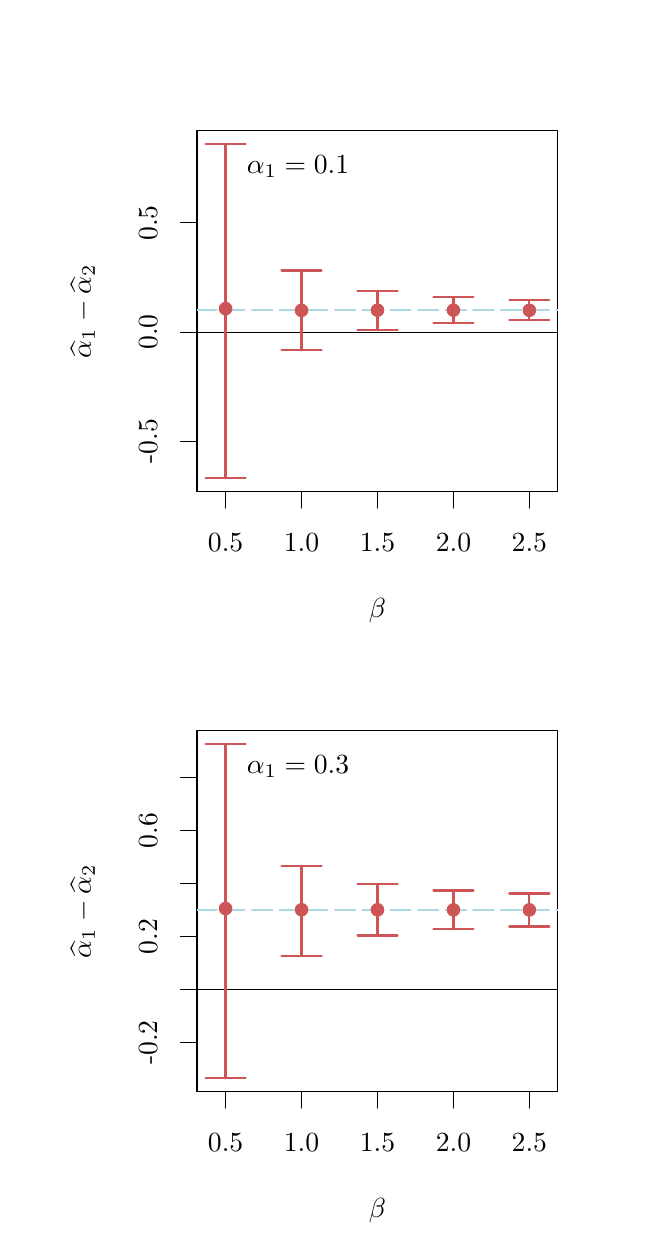
\begin{tikzpicture}[x=1pt,y=1pt]
\definecolor{fillColor}{RGB}{255,255,255}
\path[use as bounding box,fill=fillColor,fill opacity=0.00] (0,0) rectangle (216.81,433.62);
\begin{scope}
\path[clip] ( 61.20,266.01) rectangle (191.61,396.42);
\definecolor{drawColor}{RGB}{255,255,255}
\definecolor{fillColor}{RGB}{255,255,255}

\path[draw=drawColor,line width= 0.4pt,line join=round,line cap=round,fill=fillColor] ( 71.52,332.09) circle (  2.25);

\path[draw=drawColor,line width= 0.4pt,line join=round,line cap=round,fill=fillColor] ( 98.96,331.46) circle (  2.25);

\path[draw=drawColor,line width= 0.4pt,line join=round,line cap=round,fill=fillColor] (126.40,331.52) circle (  2.25);

\path[draw=drawColor,line width= 0.4pt,line join=round,line cap=round,fill=fillColor] (153.85,331.53) circle (  2.25);

\path[draw=drawColor,line width= 0.4pt,line join=round,line cap=round,fill=fillColor] (181.29,331.48) circle (  2.25);
\end{scope}
\begin{scope}
\path[clip] (  0.00,  0.00) rectangle (216.81,433.62);
\definecolor{drawColor}{RGB}{0,0,0}

\path[draw=drawColor,line width= 0.4pt,line join=round,line cap=round] ( 71.52,266.01) -- (181.29,266.01);

\path[draw=drawColor,line width= 0.4pt,line join=round,line cap=round] ( 71.52,266.01) -- ( 71.52,260.01);

\path[draw=drawColor,line width= 0.4pt,line join=round,line cap=round] ( 98.96,266.01) -- ( 98.96,260.01);

\path[draw=drawColor,line width= 0.4pt,line join=round,line cap=round] (126.40,266.01) -- (126.40,260.01);

\path[draw=drawColor,line width= 0.4pt,line join=round,line cap=round] (153.85,266.01) -- (153.85,260.01);

\path[draw=drawColor,line width= 0.4pt,line join=round,line cap=round] (181.29,266.01) -- (181.29,260.01);

\node[text=drawColor,anchor=base,inner sep=0pt, outer sep=0pt, scale=  1.00] at ( 71.52,244.41) {0.5};

\node[text=drawColor,anchor=base,inner sep=0pt, outer sep=0pt, scale=  1.00] at ( 98.96,244.41) {1.0};

\node[text=drawColor,anchor=base,inner sep=0pt, outer sep=0pt, scale=  1.00] at (126.40,244.41) {1.5};

\node[text=drawColor,anchor=base,inner sep=0pt, outer sep=0pt, scale=  1.00] at (153.85,244.41) {2.0};

\node[text=drawColor,anchor=base,inner sep=0pt, outer sep=0pt, scale=  1.00] at (181.29,244.41) {2.5};

\path[draw=drawColor,line width= 0.4pt,line join=round,line cap=round] ( 61.20,284.18) -- ( 61.20,363.07);

\path[draw=drawColor,line width= 0.4pt,line join=round,line cap=round] ( 61.20,284.18) -- ( 55.20,284.18);

\path[draw=drawColor,line width= 0.4pt,line join=round,line cap=round] ( 61.20,323.62) -- ( 55.20,323.62);

\path[draw=drawColor,line width= 0.4pt,line join=round,line cap=round] ( 61.20,363.07) -- ( 55.20,363.07);

\node[text=drawColor,rotate= 90.00,anchor=base,inner sep=0pt, outer sep=0pt, scale=  1.00] at ( 46.80,284.18) {-0.5};

\node[text=drawColor,rotate= 90.00,anchor=base,inner sep=0pt, outer sep=0pt, scale=  1.00] at ( 46.80,323.62) {0.0};

\node[text=drawColor,rotate= 90.00,anchor=base,inner sep=0pt, outer sep=0pt, scale=  1.00] at ( 46.80,363.07) {0.5};

\path[draw=drawColor,line width= 0.4pt,line join=round,line cap=round] ( 61.20,266.01) --
	(191.61,266.01) --
	(191.61,396.42) --
	( 61.20,396.42) --
	( 61.20,266.01);
\end{scope}
\begin{scope}
\path[clip] (  0.00,216.81) rectangle (216.81,433.62);
\definecolor{drawColor}{RGB}{0,0,0}

\node[text=drawColor,anchor=base,inner sep=0pt, outer sep=0pt, scale=  1.00] at (126.41,220.41) {$\beta$};

\node[text=drawColor,rotate= 90.00,anchor=base,inner sep=0pt, outer sep=0pt, scale=  1.00] at ( 22.80,331.22) {$\widehat{\alpha}_1 - \widehat{\alpha}_2$};
\end{scope}
\begin{scope}
\path[clip] ( 61.20,266.01) rectangle (191.61,396.42);
\definecolor{drawColor}{RGB}{0,0,0}

\node[text=drawColor,anchor=base west,inner sep=0pt, outer sep=0pt, scale=  1.00] at ( 79.20,380.98) {$\alpha_1=0.1$};
\definecolor{drawColor}{RGB}{173,216,230}

\path[draw=drawColor,line width= 0.8pt,dash pattern=on 7pt off 3pt ,line join=round,line cap=round] ( 61.20,331.51) -- (191.61,331.51);

\path[draw=drawColor,line width= 0.8pt,dash pattern=on 7pt off 3pt ,line join=round,line cap=round] ( 61.20,331.51) -- (191.61,331.51);

\path[draw=drawColor,line width= 0.8pt,dash pattern=on 7pt off 3pt ,line join=round,line cap=round] ( 61.20,331.51) -- (191.61,331.51);

\path[draw=drawColor,line width= 0.8pt,dash pattern=on 7pt off 3pt ,line join=round,line cap=round] ( 61.20,331.51) -- (191.61,331.51);

\path[draw=drawColor,line width= 0.8pt,dash pattern=on 7pt off 3pt ,line join=round,line cap=round] ( 61.20,331.51) -- (191.61,331.51);
\definecolor{drawColor}{RGB}{0,0,0}

\path[draw=drawColor,line width= 0.4pt,line join=round,line cap=round] ( 61.20,323.62) -- (191.61,323.62);
\definecolor{drawColor}{RGB}{205,85,85}

\path[draw=drawColor,line width= 0.8pt,line join=round,line cap=round] ( 71.52,270.84) -- ( 71.52,391.59);

\path[draw=drawColor,line width= 0.8pt,line join=round,line cap=round] ( 64.29,270.84) --
	( 71.52,270.84) --
	( 78.75,270.84);

\path[draw=drawColor,line width= 0.8pt,line join=round,line cap=round] ( 78.75,391.59) --
	( 71.52,391.59) --
	( 64.29,391.59);

\path[draw=drawColor,line width= 0.8pt,line join=round,line cap=round] ( 98.96,317.03) -- ( 98.96,345.88);

\path[draw=drawColor,line width= 0.8pt,line join=round,line cap=round] ( 91.73,317.03) --
	( 98.96,317.03) --
	(106.19,317.03);

\path[draw=drawColor,line width= 0.8pt,line join=round,line cap=round] (106.19,345.88) --
	( 98.96,345.88) --
	( 91.73,345.88);

\path[draw=drawColor,line width= 0.8pt,line join=round,line cap=round] (126.40,324.38) -- (126.40,338.56);

\path[draw=drawColor,line width= 0.8pt,line join=round,line cap=round] (119.18,324.38) --
	(126.40,324.38) --
	(133.63,324.38);

\path[draw=drawColor,line width= 0.8pt,line join=round,line cap=round] (133.63,338.56) --
	(126.40,338.56) --
	(119.18,338.56);

\path[draw=drawColor,line width= 0.8pt,line join=round,line cap=round] (153.85,326.78) -- (153.85,336.30);

\path[draw=drawColor,line width= 0.8pt,line join=round,line cap=round] (146.62,326.78) --
	(153.85,326.78) --
	(161.08,326.78);

\path[draw=drawColor,line width= 0.8pt,line join=round,line cap=round] (161.08,336.30) --
	(153.85,336.30) --
	(146.62,336.30);

\path[draw=drawColor,line width= 0.8pt,line join=round,line cap=round] (181.29,327.85) -- (181.29,335.20);

\path[draw=drawColor,line width= 0.8pt,line join=round,line cap=round] (174.06,327.85) --
	(181.29,327.85) --
	(188.52,327.85);

\path[draw=drawColor,line width= 0.8pt,line join=round,line cap=round] (188.52,335.20) --
	(181.29,335.20) --
	(174.06,335.20);
\definecolor{fillColor}{RGB}{205,85,85}

\path[draw=drawColor,line width= 0.4pt,line join=round,line cap=round,fill=fillColor] ( 71.52,332.09) circle (  2.25);

\path[draw=drawColor,line width= 0.4pt,line join=round,line cap=round,fill=fillColor] ( 98.96,331.46) circle (  2.25);

\path[draw=drawColor,line width= 0.4pt,line join=round,line cap=round,fill=fillColor] (126.40,331.52) circle (  2.25);

\path[draw=drawColor,line width= 0.4pt,line join=round,line cap=round,fill=fillColor] (153.85,331.53) circle (  2.25);

\path[draw=drawColor,line width= 0.4pt,line join=round,line cap=round,fill=fillColor] (181.29,331.48) circle (  2.25);
\end{scope}
\begin{scope}
\path[clip] ( 61.20, 49.20) rectangle (191.61,179.61);
\definecolor{drawColor}{RGB}{255,255,255}
\definecolor{fillColor}{RGB}{255,255,255}

\path[draw=drawColor,line width= 0.4pt,line join=round,line cap=round,fill=fillColor] ( 71.52,115.33) circle (  2.25);

\path[draw=drawColor,line width= 0.4pt,line join=round,line cap=round,fill=fillColor] ( 98.96,114.88) circle (  2.25);

\path[draw=drawColor,line width= 0.4pt,line join=round,line cap=round,fill=fillColor] (126.40,114.87) circle (  2.25);

\path[draw=drawColor,line width= 0.4pt,line join=round,line cap=round,fill=fillColor] (153.85,114.83) circle (  2.25);

\path[draw=drawColor,line width= 0.4pt,line join=round,line cap=round,fill=fillColor] (181.29,114.84) circle (  2.25);
\end{scope}
\begin{scope}
\path[clip] (  0.00,  0.00) rectangle (216.81,433.62);
\definecolor{drawColor}{RGB}{0,0,0}

\path[draw=drawColor,line width= 0.4pt,line join=round,line cap=round] ( 71.52, 49.20) -- (181.29, 49.20);

\path[draw=drawColor,line width= 0.4pt,line join=round,line cap=round] ( 71.52, 49.20) -- ( 71.52, 43.20);

\path[draw=drawColor,line width= 0.4pt,line join=round,line cap=round] ( 98.96, 49.20) -- ( 98.96, 43.20);

\path[draw=drawColor,line width= 0.4pt,line join=round,line cap=round] (126.40, 49.20) -- (126.40, 43.20);

\path[draw=drawColor,line width= 0.4pt,line join=round,line cap=round] (153.85, 49.20) -- (153.85, 43.20);

\path[draw=drawColor,line width= 0.4pt,line join=round,line cap=round] (181.29, 49.20) -- (181.29, 43.20);

\node[text=drawColor,anchor=base,inner sep=0pt, outer sep=0pt, scale=  1.00] at ( 71.52, 27.60) {0.5};

\node[text=drawColor,anchor=base,inner sep=0pt, outer sep=0pt, scale=  1.00] at ( 98.96, 27.60) {1.0};

\node[text=drawColor,anchor=base,inner sep=0pt, outer sep=0pt, scale=  1.00] at (126.40, 27.60) {1.5};

\node[text=drawColor,anchor=base,inner sep=0pt, outer sep=0pt, scale=  1.00] at (153.85, 27.60) {2.0};

\node[text=drawColor,anchor=base,inner sep=0pt, outer sep=0pt, scale=  1.00] at (181.29, 27.60) {2.5};

\path[draw=drawColor,line width= 0.4pt,line join=round,line cap=round] ( 61.20, 66.91) -- ( 61.20,162.74);

\path[draw=drawColor,line width= 0.4pt,line join=round,line cap=round] ( 61.20, 66.91) -- ( 55.20, 66.91);

\path[draw=drawColor,line width= 0.4pt,line join=round,line cap=round] ( 61.20, 86.08) -- ( 55.20, 86.08);

\path[draw=drawColor,line width= 0.4pt,line join=round,line cap=round] ( 61.20,105.24) -- ( 55.20,105.24);

\path[draw=drawColor,line width= 0.4pt,line join=round,line cap=round] ( 61.20,124.41) -- ( 55.20,124.41);

\path[draw=drawColor,line width= 0.4pt,line join=round,line cap=round] ( 61.20,143.57) -- ( 55.20,143.57);

\path[draw=drawColor,line width= 0.4pt,line join=round,line cap=round] ( 61.20,162.74) -- ( 55.20,162.74);

\node[text=drawColor,rotate= 90.00,anchor=base,inner sep=0pt, outer sep=0pt, scale=  1.00] at ( 46.80, 66.91) {-0.2};

\node[text=drawColor,rotate= 90.00,anchor=base,inner sep=0pt, outer sep=0pt, scale=  1.00] at ( 46.80,105.24) {0.2};

\node[text=drawColor,rotate= 90.00,anchor=base,inner sep=0pt, outer sep=0pt, scale=  1.00] at ( 46.80,143.57) {0.6};

\path[draw=drawColor,line width= 0.4pt,line join=round,line cap=round] ( 61.20, 49.20) --
	(191.61, 49.20) --
	(191.61,179.61) --
	( 61.20,179.61) --
	( 61.20, 49.20);
\end{scope}
\begin{scope}
\path[clip] (  0.00,  0.00) rectangle (216.81,216.81);
\definecolor{drawColor}{RGB}{0,0,0}

\node[text=drawColor,anchor=base,inner sep=0pt, outer sep=0pt, scale=  1.00] at (126.41,  3.60) {$\beta$};

\node[text=drawColor,rotate= 90.00,anchor=base,inner sep=0pt, outer sep=0pt, scale=  1.00] at ( 22.80,114.41) {$\widehat{\alpha}_1 - \widehat{\alpha}_2$};
\end{scope}
\begin{scope}
\path[clip] ( 61.20, 49.20) rectangle (191.61,179.61);
\definecolor{drawColor}{RGB}{0,0,0}

\node[text=drawColor,anchor=base west,inner sep=0pt, outer sep=0pt, scale=  1.00] at ( 79.20,164.17) {$\alpha_1=0.3$};
\definecolor{drawColor}{RGB}{173,216,230}

\path[draw=drawColor,line width= 0.8pt,dash pattern=on 7pt off 3pt ,line join=round,line cap=round] ( 61.20,114.82) -- (191.61,114.82);

\path[draw=drawColor,line width= 0.8pt,dash pattern=on 7pt off 3pt ,line join=round,line cap=round] ( 61.20,114.82) -- (191.61,114.82);

\path[draw=drawColor,line width= 0.8pt,dash pattern=on 7pt off 3pt ,line join=round,line cap=round] ( 61.20,114.82) -- (191.61,114.82);

\path[draw=drawColor,line width= 0.8pt,dash pattern=on 7pt off 3pt ,line join=round,line cap=round] ( 61.20,114.82) -- (191.61,114.82);

\path[draw=drawColor,line width= 0.8pt,dash pattern=on 7pt off 3pt ,line join=round,line cap=round] ( 61.20,114.82) -- (191.61,114.82);
\definecolor{drawColor}{RGB}{0,0,0}

\path[draw=drawColor,line width= 0.4pt,line join=round,line cap=round] ( 61.20, 86.08) -- (191.61, 86.08);
\definecolor{drawColor}{RGB}{205,85,85}

\path[draw=drawColor,line width= 0.8pt,line join=round,line cap=round] ( 71.52, 54.03) -- ( 71.52,174.78);

\path[draw=drawColor,line width= 0.8pt,line join=round,line cap=round] ( 64.29, 54.03) --
	( 71.52, 54.03) --
	( 78.75, 54.03);

\path[draw=drawColor,line width= 0.8pt,line join=round,line cap=round] ( 78.75,174.78) --
	( 71.52,174.78) --
	( 64.29,174.78);

\path[draw=drawColor,line width= 0.8pt,line join=round,line cap=round] ( 98.96, 98.15) -- ( 98.96,130.74);

\path[draw=drawColor,line width= 0.8pt,line join=round,line cap=round] ( 91.73, 98.15) --
	( 98.96, 98.15) --
	(106.19, 98.15);

\path[draw=drawColor,line width= 0.8pt,line join=round,line cap=round] (106.19,130.74) --
	( 98.96,130.74) --
	( 91.73,130.74);

\path[draw=drawColor,line width= 0.8pt,line join=round,line cap=round] (126.40,105.56) -- (126.40,124.15);

\path[draw=drawColor,line width= 0.8pt,line join=round,line cap=round] (119.18,105.56) --
	(126.40,105.56) --
	(133.63,105.56);

\path[draw=drawColor,line width= 0.8pt,line join=round,line cap=round] (133.63,124.15) --
	(126.40,124.15) --
	(119.18,124.15);

\path[draw=drawColor,line width= 0.8pt,line join=round,line cap=round] (153.85,107.85) -- (153.85,121.82);

\path[draw=drawColor,line width= 0.8pt,line join=round,line cap=round] (146.62,107.85) --
	(153.85,107.85) --
	(161.08,107.85);

\path[draw=drawColor,line width= 0.8pt,line join=round,line cap=round] (161.08,121.82) --
	(153.85,121.82) --
	(146.62,121.82);

\path[draw=drawColor,line width= 0.8pt,line join=round,line cap=round] (181.29,108.83) -- (181.29,120.74);

\path[draw=drawColor,line width= 0.8pt,line join=round,line cap=round] (174.06,108.83) --
	(181.29,108.83) --
	(188.52,108.83);

\path[draw=drawColor,line width= 0.8pt,line join=round,line cap=round] (188.52,120.74) --
	(181.29,120.74) --
	(174.06,120.74);
\definecolor{fillColor}{RGB}{205,85,85}

\path[draw=drawColor,line width= 0.4pt,line join=round,line cap=round,fill=fillColor] ( 71.52,115.33) circle (  2.25);

\path[draw=drawColor,line width= 0.4pt,line join=round,line cap=round,fill=fillColor] ( 98.96,114.88) circle (  2.25);

\path[draw=drawColor,line width= 0.4pt,line join=round,line cap=round,fill=fillColor] (126.40,114.87) circle (  2.25);

\path[draw=drawColor,line width= 0.4pt,line join=round,line cap=round,fill=fillColor] (153.85,114.83) circle (  2.25);

\path[draw=drawColor,line width= 0.4pt,line join=round,line cap=round,fill=fillColor] (181.29,114.84) circle (  2.25);
\end{scope}
\end{tikzpicture}

%  \end{subfigure}
%  ~
%  \begin{subfigure}[b]{0.31\textwidth}
%\caption{\footnotesize $N=5000, \delta = 0.1$}
%  % Created by tikzDevice version 0.8.1 on 2015-11-17 12:44:46
% !TEX encoding = UTF-8 Unicode
\begin{tikzpicture}[x=1pt,y=1pt]
\definecolor{fillColor}{RGB}{255,255,255}
\path[use as bounding box,fill=fillColor,fill opacity=0.00] (0,0) rectangle (216.81,433.62);
\begin{scope}
\path[clip] (  0.00,  0.00) rectangle (216.81,433.62);
\definecolor{drawColor}{RGB}{0,0,0}

\path[draw=drawColor,line width= 0.4pt,line join=round,line cap=round] ( 71.52,266.01) -- (181.29,266.01);

\path[draw=drawColor,line width= 0.4pt,line join=round,line cap=round] ( 71.52,266.01) -- ( 71.52,260.01);

\path[draw=drawColor,line width= 0.4pt,line join=round,line cap=round] ( 98.96,266.01) -- ( 98.96,260.01);

\path[draw=drawColor,line width= 0.4pt,line join=round,line cap=round] (126.40,266.01) -- (126.40,260.01);

\path[draw=drawColor,line width= 0.4pt,line join=round,line cap=round] (153.85,266.01) -- (153.85,260.01);

\path[draw=drawColor,line width= 0.4pt,line join=round,line cap=round] (181.29,266.01) -- (181.29,260.01);

\node[text=drawColor,anchor=base,inner sep=0pt, outer sep=0pt, scale=  1.00] at ( 71.52,244.41) {0.5};

\node[text=drawColor,anchor=base,inner sep=0pt, outer sep=0pt, scale=  1.00] at ( 98.96,244.41) {1.0};

\node[text=drawColor,anchor=base,inner sep=0pt, outer sep=0pt, scale=  1.00] at (126.40,244.41) {1.5};

\node[text=drawColor,anchor=base,inner sep=0pt, outer sep=0pt, scale=  1.00] at (153.85,244.41) {2.0};

\node[text=drawColor,anchor=base,inner sep=0pt, outer sep=0pt, scale=  1.00] at (181.29,244.41) {2.5};

\path[draw=drawColor,line width= 0.4pt,line join=round,line cap=round] ( 61.20,266.01) --
	(191.61,266.01) --
	(191.61,396.42) --
	( 61.20,396.42) --
	( 61.20,266.01);
\end{scope}
\begin{scope}
\path[clip] (  0.00,216.81) rectangle (216.81,433.62);
\definecolor{drawColor}{RGB}{0,0,0}

\node[text=drawColor,anchor=base,inner sep=0pt, outer sep=0pt, scale=  1.00] at (126.41,220.41) {$\beta$};

\node[text=drawColor,rotate= 90.00,anchor=base,inner sep=0pt, outer sep=0pt, scale=  1.00] at ( 22.80,331.22) {$\widehat{\alpha}_1 - \widehat{\alpha}_0$};
\end{scope}
\begin{scope}
\path[clip] (  0.00,  0.00) rectangle (216.81,433.62);
\definecolor{drawColor}{RGB}{0,0,0}

\path[draw=drawColor,line width= 0.4pt,line join=round,line cap=round] ( 61.20,270.84) -- ( 61.20,391.59);

\path[draw=drawColor,line width= 0.4pt,line join=round,line cap=round] ( 61.20,270.84) -- ( 55.20,270.84);

\path[draw=drawColor,line width= 0.4pt,line join=round,line cap=round] ( 61.20,301.03) -- ( 55.20,301.03);

\path[draw=drawColor,line width= 0.4pt,line join=round,line cap=round] ( 61.20,331.22) -- ( 55.20,331.22);

\path[draw=drawColor,line width= 0.4pt,line join=round,line cap=round] ( 61.20,361.40) -- ( 55.20,361.40);

\path[draw=drawColor,line width= 0.4pt,line join=round,line cap=round] ( 61.20,391.59) -- ( 55.20,391.59);

\node[text=drawColor,rotate= 90.00,anchor=base,inner sep=0pt, outer sep=0pt, scale=  1.00] at ( 46.80,270.84) {-1};

\node[text=drawColor,rotate= 90.00,anchor=base,inner sep=0pt, outer sep=0pt, scale=  1.00] at ( 46.80,331.22) {0};

\node[text=drawColor,rotate= 90.00,anchor=base,inner sep=0pt, outer sep=0pt, scale=  1.00] at ( 46.80,391.59) {1};
\end{scope}
\begin{scope}
\path[clip] ( 61.20,266.01) rectangle (191.61,396.42);
\definecolor{drawColor}{RGB}{0,0,0}

\node[text=drawColor,anchor=base west,inner sep=0pt, outer sep=0pt, scale=  1.00] at (114.66,380.98) {$\alpha_1=0.1$};
\definecolor{drawColor}{RGB}{173,216,230}

\path[draw=drawColor,line width= 0.8pt,dash pattern=on 7pt off 3pt ,line join=round,line cap=round] ( 61.20,337.25) -- (191.61,337.25);

\path[draw=drawColor,line width= 0.8pt,dash pattern=on 7pt off 3pt ,line join=round,line cap=round] ( 61.20,337.25) -- (191.61,337.25);

\path[draw=drawColor,line width= 0.8pt,dash pattern=on 7pt off 3pt ,line join=round,line cap=round] ( 61.20,337.25) -- (191.61,337.25);

\path[draw=drawColor,line width= 0.8pt,dash pattern=on 7pt off 3pt ,line join=round,line cap=round] ( 61.20,337.25) -- (191.61,337.25);

\path[draw=drawColor,line width= 0.8pt,dash pattern=on 7pt off 3pt ,line join=round,line cap=round] ( 61.20,337.25) -- (191.61,337.25);
\definecolor{drawColor}{RGB}{0,0,0}

\path[draw=drawColor,line width= 0.4pt,line join=round,line cap=round] ( 61.20,331.22) -- (191.61,331.22);
\definecolor{drawColor}{RGB}{205,85,85}

\path[draw=drawColor,line width= 0.8pt,line join=round,line cap=round] ( 71.52,318.63) -- ( 71.52,355.64);

\path[draw=drawColor,line width= 0.8pt,line join=round,line cap=round] ( 64.29,318.63) --
	( 71.52,318.63) --
	( 78.75,318.63);

\path[draw=drawColor,line width= 0.8pt,line join=round,line cap=round] ( 78.75,355.64) --
	( 71.52,355.64) --
	( 64.29,355.64);

\path[draw=drawColor,line width= 0.8pt,line join=round,line cap=round] ( 98.96,332.42) -- ( 98.96,342.10);

\path[draw=drawColor,line width= 0.8pt,line join=round,line cap=round] ( 91.73,332.42) --
	( 98.96,332.42) --
	(106.19,332.42);

\path[draw=drawColor,line width= 0.8pt,line join=round,line cap=round] (106.19,342.10) --
	( 98.96,342.10) --
	( 91.73,342.10);

\path[draw=drawColor,line width= 0.8pt,line join=round,line cap=round] (126.40,334.84) -- (126.40,339.63);

\path[draw=drawColor,line width= 0.8pt,line join=round,line cap=round] (119.18,334.84) --
	(126.40,334.84) --
	(133.63,334.84);

\path[draw=drawColor,line width= 0.8pt,line join=round,line cap=round] (133.63,339.63) --
	(126.40,339.63) --
	(119.18,339.63);

\path[draw=drawColor,line width= 0.8pt,line join=round,line cap=round] (153.85,335.65) -- (153.85,338.84);

\path[draw=drawColor,line width= 0.8pt,line join=round,line cap=round] (146.62,335.65) --
	(153.85,335.65) --
	(161.08,335.65);

\path[draw=drawColor,line width= 0.8pt,line join=round,line cap=round] (161.08,338.84) --
	(153.85,338.84) --
	(146.62,338.84);

\path[draw=drawColor,line width= 0.8pt,line join=round,line cap=round] (181.29,336.03) -- (181.29,338.49);

\path[draw=drawColor,line width= 0.8pt,line join=round,line cap=round] (174.06,336.03) --
	(181.29,336.03) --
	(188.52,336.03);

\path[draw=drawColor,line width= 0.8pt,line join=round,line cap=round] (188.52,338.49) --
	(181.29,338.49) --
	(174.06,338.49);
\definecolor{fillColor}{RGB}{205,85,85}

\path[draw=drawColor,line width= 0.4pt,line join=round,line cap=round,fill=fillColor] ( 71.52,337.05) circle (  2.25);

\path[draw=drawColor,line width= 0.4pt,line join=round,line cap=round,fill=fillColor] ( 98.96,337.27) circle (  2.25);

\path[draw=drawColor,line width= 0.4pt,line join=round,line cap=round,fill=fillColor] (126.40,337.24) circle (  2.25);

\path[draw=drawColor,line width= 0.4pt,line join=round,line cap=round,fill=fillColor] (153.85,337.27) circle (  2.25);

\path[draw=drawColor,line width= 0.4pt,line join=round,line cap=round,fill=fillColor] (181.29,337.24) circle (  2.25);
\end{scope}
\begin{scope}
\path[clip] (  0.00,  0.00) rectangle (216.81,433.62);
\definecolor{drawColor}{RGB}{0,0,0}

\path[draw=drawColor,line width= 0.4pt,line join=round,line cap=round] ( 71.52, 49.20) -- (181.29, 49.20);

\path[draw=drawColor,line width= 0.4pt,line join=round,line cap=round] ( 71.52, 49.20) -- ( 71.52, 43.20);

\path[draw=drawColor,line width= 0.4pt,line join=round,line cap=round] ( 98.96, 49.20) -- ( 98.96, 43.20);

\path[draw=drawColor,line width= 0.4pt,line join=round,line cap=round] (126.40, 49.20) -- (126.40, 43.20);

\path[draw=drawColor,line width= 0.4pt,line join=round,line cap=round] (153.85, 49.20) -- (153.85, 43.20);

\path[draw=drawColor,line width= 0.4pt,line join=round,line cap=round] (181.29, 49.20) -- (181.29, 43.20);

\node[text=drawColor,anchor=base,inner sep=0pt, outer sep=0pt, scale=  1.00] at ( 71.52, 27.60) {0.5};

\node[text=drawColor,anchor=base,inner sep=0pt, outer sep=0pt, scale=  1.00] at ( 98.96, 27.60) {1.0};

\node[text=drawColor,anchor=base,inner sep=0pt, outer sep=0pt, scale=  1.00] at (126.40, 27.60) {1.5};

\node[text=drawColor,anchor=base,inner sep=0pt, outer sep=0pt, scale=  1.00] at (153.85, 27.60) {2.0};

\node[text=drawColor,anchor=base,inner sep=0pt, outer sep=0pt, scale=  1.00] at (181.29, 27.60) {2.5};

\path[draw=drawColor,line width= 0.4pt,line join=round,line cap=round] ( 61.20, 49.20) --
	(191.61, 49.20) --
	(191.61,179.61) --
	( 61.20,179.61) --
	( 61.20, 49.20);
\end{scope}
\begin{scope}
\path[clip] (  0.00,  0.00) rectangle (216.81,216.81);
\definecolor{drawColor}{RGB}{0,0,0}

\node[text=drawColor,anchor=base,inner sep=0pt, outer sep=0pt, scale=  1.00] at (126.41,  3.60) {$\beta$};

\node[text=drawColor,rotate= 90.00,anchor=base,inner sep=0pt, outer sep=0pt, scale=  1.00] at ( 22.80,114.41) {$\widehat{\alpha}_1 - \widehat{\alpha}_0$};
\end{scope}
\begin{scope}
\path[clip] (  0.00,  0.00) rectangle (216.81,433.62);
\definecolor{drawColor}{RGB}{0,0,0}

\path[draw=drawColor,line width= 0.4pt,line join=round,line cap=round] ( 61.20, 54.03) -- ( 61.20,174.78);

\path[draw=drawColor,line width= 0.4pt,line join=round,line cap=round] ( 61.20, 54.03) -- ( 55.20, 54.03);

\path[draw=drawColor,line width= 0.4pt,line join=round,line cap=round] ( 61.20, 84.22) -- ( 55.20, 84.22);

\path[draw=drawColor,line width= 0.4pt,line join=round,line cap=round] ( 61.20,114.41) -- ( 55.20,114.41);

\path[draw=drawColor,line width= 0.4pt,line join=round,line cap=round] ( 61.20,144.59) -- ( 55.20,144.59);

\path[draw=drawColor,line width= 0.4pt,line join=round,line cap=round] ( 61.20,174.78) -- ( 55.20,174.78);

\node[text=drawColor,rotate= 90.00,anchor=base,inner sep=0pt, outer sep=0pt, scale=  1.00] at ( 46.80, 54.03) {-1};

\node[text=drawColor,rotate= 90.00,anchor=base,inner sep=0pt, outer sep=0pt, scale=  1.00] at ( 46.80,114.41) {0};

\node[text=drawColor,rotate= 90.00,anchor=base,inner sep=0pt, outer sep=0pt, scale=  1.00] at ( 46.80,174.78) {1};
\end{scope}
\begin{scope}
\path[clip] ( 61.20, 49.20) rectangle (191.61,179.61);
\definecolor{drawColor}{RGB}{0,0,0}

\node[text=drawColor,anchor=base west,inner sep=0pt, outer sep=0pt, scale=  1.00] at (114.66,164.17) {$\alpha_1=0.3$};
\definecolor{drawColor}{RGB}{173,216,230}

\path[draw=drawColor,line width= 0.8pt,dash pattern=on 7pt off 3pt ,line join=round,line cap=round] ( 61.20,132.52) -- (191.61,132.52);

\path[draw=drawColor,line width= 0.8pt,dash pattern=on 7pt off 3pt ,line join=round,line cap=round] ( 61.20,132.52) -- (191.61,132.52);

\path[draw=drawColor,line width= 0.8pt,dash pattern=on 7pt off 3pt ,line join=round,line cap=round] ( 61.20,132.52) -- (191.61,132.52);

\path[draw=drawColor,line width= 0.8pt,dash pattern=on 7pt off 3pt ,line join=round,line cap=round] ( 61.20,132.52) -- (191.61,132.52);

\path[draw=drawColor,line width= 0.8pt,dash pattern=on 7pt off 3pt ,line join=round,line cap=round] ( 61.20,132.52) -- (191.61,132.52);
\definecolor{drawColor}{RGB}{0,0,0}

\path[draw=drawColor,line width= 0.4pt,line join=round,line cap=round] ( 61.20,114.41) -- (191.61,114.41);
\definecolor{drawColor}{RGB}{205,85,85}

\path[draw=drawColor,line width= 0.8pt,line join=round,line cap=round] ( 71.52,117.45) -- ( 71.52,147.78);

\path[draw=drawColor,line width= 0.8pt,line join=round,line cap=round] ( 64.29,117.45) --
	( 71.52,117.45) --
	( 78.75,117.45);

\path[draw=drawColor,line width= 0.8pt,line join=round,line cap=round] ( 78.75,147.78) --
	( 71.52,147.78) --
	( 64.29,147.78);

\path[draw=drawColor,line width= 0.8pt,line join=round,line cap=round] ( 98.96,128.11) -- ( 98.96,136.93);

\path[draw=drawColor,line width= 0.8pt,line join=round,line cap=round] ( 91.73,128.11) --
	( 98.96,128.11) --
	(106.19,128.11);

\path[draw=drawColor,line width= 0.8pt,line join=round,line cap=round] (106.19,136.93) --
	( 98.96,136.93) --
	( 91.73,136.93);

\path[draw=drawColor,line width= 0.8pt,line join=round,line cap=round] (126.40,129.95) -- (126.40,135.07);

\path[draw=drawColor,line width= 0.8pt,line join=round,line cap=round] (119.18,129.95) --
	(126.40,129.95) --
	(133.63,129.95);

\path[draw=drawColor,line width= 0.8pt,line join=round,line cap=round] (133.63,135.07) --
	(126.40,135.07) --
	(119.18,135.07);

\path[draw=drawColor,line width= 0.8pt,line join=round,line cap=round] (153.85,130.56) -- (153.85,134.42);

\path[draw=drawColor,line width= 0.8pt,line join=round,line cap=round] (146.62,130.56) --
	(153.85,130.56) --
	(161.08,130.56);

\path[draw=drawColor,line width= 0.8pt,line join=round,line cap=round] (161.08,134.42) --
	(153.85,134.42) --
	(146.62,134.42);

\path[draw=drawColor,line width= 0.8pt,line join=round,line cap=round] (181.29,130.84) -- (181.29,134.22);

\path[draw=drawColor,line width= 0.8pt,line join=round,line cap=round] (174.06,130.84) --
	(181.29,130.84) --
	(188.52,130.84);

\path[draw=drawColor,line width= 0.8pt,line join=round,line cap=round] (188.52,134.22) --
	(181.29,134.22) --
	(174.06,134.22);
\definecolor{fillColor}{RGB}{205,85,85}

\path[draw=drawColor,line width= 0.4pt,line join=round,line cap=round,fill=fillColor] ( 71.52,132.66) circle (  2.25);

\path[draw=drawColor,line width= 0.4pt,line join=round,line cap=round,fill=fillColor] ( 98.96,132.50) circle (  2.25);

\path[draw=drawColor,line width= 0.4pt,line join=round,line cap=round,fill=fillColor] (126.40,132.53) circle (  2.25);

\path[draw=drawColor,line width= 0.4pt,line join=round,line cap=round,fill=fillColor] (153.85,132.48) circle (  2.25);

\path[draw=drawColor,line width= 0.4pt,line join=round,line cap=round,fill=fillColor] (181.29,132.52) circle (  2.25);
\end{scope}
\end{tikzpicture}

%  \end{subfigure}
%\endgroup
%\end{figure}
%\end{frame}
%%%%%%%%%%%%%%%%%%%%%%%%%%%%%%%%%%%%%%
%\begin{frame}
%\begin{figure}[h]
%  \scriptsize
%  \begingroup
%  \tikzset{every picture/.style={scale=0.53}}
%  \centering
%  \begin{subfigure}[b]{0.31\textwidth}
%\caption{\footnotesize $N=500, \delta = 0.2$}
%  % Created by tikzDevice version 0.8.1 on 2015-11-17 11:43:47
% !TEX encoding = UTF-8 Unicode
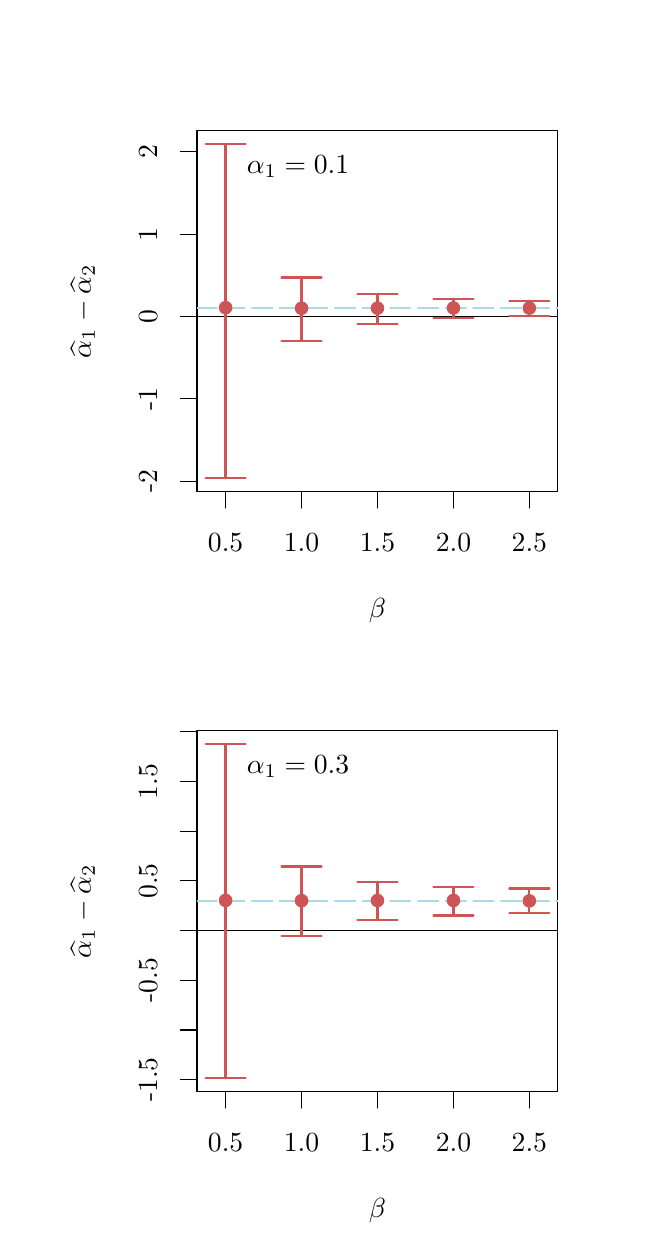
\begin{tikzpicture}[x=1pt,y=1pt]
\definecolor{fillColor}{RGB}{255,255,255}
\path[use as bounding box,fill=fillColor,fill opacity=0.00] (0,0) rectangle (216.81,433.62);
\begin{scope}
\path[clip] ( 61.20,266.01) rectangle (191.61,396.42);
\definecolor{drawColor}{RGB}{255,255,255}
\definecolor{fillColor}{RGB}{255,255,255}

\path[draw=drawColor,line width= 0.4pt,line join=round,line cap=round,fill=fillColor] ( 71.52,332.44) circle (  2.25);

\path[draw=drawColor,line width= 0.4pt,line join=round,line cap=round,fill=fillColor] ( 98.96,332.22) circle (  2.25);

\path[draw=drawColor,line width= 0.4pt,line join=round,line cap=round,fill=fillColor] (126.40,332.26) circle (  2.25);

\path[draw=drawColor,line width= 0.4pt,line join=round,line cap=round,fill=fillColor] (153.85,332.32) circle (  2.25);

\path[draw=drawColor,line width= 0.4pt,line join=round,line cap=round,fill=fillColor] (181.29,332.28) circle (  2.25);
\end{scope}
\begin{scope}
\path[clip] (  0.00,  0.00) rectangle (216.81,433.62);
\definecolor{drawColor}{RGB}{0,0,0}

\path[draw=drawColor,line width= 0.4pt,line join=round,line cap=round] ( 71.52,266.01) -- (181.29,266.01);

\path[draw=drawColor,line width= 0.4pt,line join=round,line cap=round] ( 71.52,266.01) -- ( 71.52,260.01);

\path[draw=drawColor,line width= 0.4pt,line join=round,line cap=round] ( 98.96,266.01) -- ( 98.96,260.01);

\path[draw=drawColor,line width= 0.4pt,line join=round,line cap=round] (126.40,266.01) -- (126.40,260.01);

\path[draw=drawColor,line width= 0.4pt,line join=round,line cap=round] (153.85,266.01) -- (153.85,260.01);

\path[draw=drawColor,line width= 0.4pt,line join=round,line cap=round] (181.29,266.01) -- (181.29,260.01);

\node[text=drawColor,anchor=base,inner sep=0pt, outer sep=0pt, scale=  1.00] at ( 71.52,244.41) {0.5};

\node[text=drawColor,anchor=base,inner sep=0pt, outer sep=0pt, scale=  1.00] at ( 98.96,244.41) {1.0};

\node[text=drawColor,anchor=base,inner sep=0pt, outer sep=0pt, scale=  1.00] at (126.40,244.41) {1.5};

\node[text=drawColor,anchor=base,inner sep=0pt, outer sep=0pt, scale=  1.00] at (153.85,244.41) {2.0};

\node[text=drawColor,anchor=base,inner sep=0pt, outer sep=0pt, scale=  1.00] at (181.29,244.41) {2.5};

\path[draw=drawColor,line width= 0.4pt,line join=round,line cap=round] ( 61.20,269.76) -- ( 61.20,388.78);

\path[draw=drawColor,line width= 0.4pt,line join=round,line cap=round] ( 61.20,269.76) -- ( 55.20,269.76);

\path[draw=drawColor,line width= 0.4pt,line join=round,line cap=round] ( 61.20,299.52) -- ( 55.20,299.52);

\path[draw=drawColor,line width= 0.4pt,line join=round,line cap=round] ( 61.20,329.27) -- ( 55.20,329.27);

\path[draw=drawColor,line width= 0.4pt,line join=round,line cap=round] ( 61.20,359.03) -- ( 55.20,359.03);

\path[draw=drawColor,line width= 0.4pt,line join=round,line cap=round] ( 61.20,388.78) -- ( 55.20,388.78);

\node[text=drawColor,rotate= 90.00,anchor=base,inner sep=0pt, outer sep=0pt, scale=  1.00] at ( 46.80,269.76) {-2};

\node[text=drawColor,rotate= 90.00,anchor=base,inner sep=0pt, outer sep=0pt, scale=  1.00] at ( 46.80,299.52) {-1};

\node[text=drawColor,rotate= 90.00,anchor=base,inner sep=0pt, outer sep=0pt, scale=  1.00] at ( 46.80,329.27) {0};

\node[text=drawColor,rotate= 90.00,anchor=base,inner sep=0pt, outer sep=0pt, scale=  1.00] at ( 46.80,359.03) {1};

\node[text=drawColor,rotate= 90.00,anchor=base,inner sep=0pt, outer sep=0pt, scale=  1.00] at ( 46.80,388.78) {2};

\path[draw=drawColor,line width= 0.4pt,line join=round,line cap=round] ( 61.20,266.01) --
	(191.61,266.01) --
	(191.61,396.42) --
	( 61.20,396.42) --
	( 61.20,266.01);
\end{scope}
\begin{scope}
\path[clip] (  0.00,216.81) rectangle (216.81,433.62);
\definecolor{drawColor}{RGB}{0,0,0}

\node[text=drawColor,anchor=base,inner sep=0pt, outer sep=0pt, scale=  1.00] at (126.41,220.41) {$\beta$};

\node[text=drawColor,rotate= 90.00,anchor=base,inner sep=0pt, outer sep=0pt, scale=  1.00] at ( 22.80,331.22) {$\widehat{\alpha}_1 - \widehat{\alpha}_2$};
\end{scope}
\begin{scope}
\path[clip] ( 61.20,266.01) rectangle (191.61,396.42);
\definecolor{drawColor}{RGB}{0,0,0}

\node[text=drawColor,anchor=base west,inner sep=0pt, outer sep=0pt, scale=  1.00] at ( 79.20,380.98) {$\alpha_1=0.1$};
\definecolor{drawColor}{RGB}{173,216,230}

\path[draw=drawColor,line width= 0.8pt,dash pattern=on 7pt off 3pt ,line join=round,line cap=round] ( 61.20,332.25) -- (191.61,332.25);

\path[draw=drawColor,line width= 0.8pt,dash pattern=on 7pt off 3pt ,line join=round,line cap=round] ( 61.20,332.25) -- (191.61,332.25);

\path[draw=drawColor,line width= 0.8pt,dash pattern=on 7pt off 3pt ,line join=round,line cap=round] ( 61.20,332.25) -- (191.61,332.25);

\path[draw=drawColor,line width= 0.8pt,dash pattern=on 7pt off 3pt ,line join=round,line cap=round] ( 61.20,332.25) -- (191.61,332.25);

\path[draw=drawColor,line width= 0.8pt,dash pattern=on 7pt off 3pt ,line join=round,line cap=round] ( 61.20,332.25) -- (191.61,332.25);
\definecolor{drawColor}{RGB}{0,0,0}

\path[draw=drawColor,line width= 0.4pt,line join=round,line cap=round] ( 61.20,329.27) -- (191.61,329.27);
\definecolor{drawColor}{RGB}{205,85,85}

\path[draw=drawColor,line width= 0.8pt,line join=round,line cap=round] ( 71.52,270.84) -- ( 71.52,391.59);

\path[draw=drawColor,line width= 0.8pt,line join=round,line cap=round] ( 64.29,270.84) --
	( 71.52,270.84) --
	( 78.75,270.84);

\path[draw=drawColor,line width= 0.8pt,line join=round,line cap=round] ( 78.75,391.59) --
	( 71.52,391.59) --
	( 64.29,391.59);

\path[draw=drawColor,line width= 0.8pt,line join=round,line cap=round] ( 98.96,320.47) -- ( 98.96,343.36);

\path[draw=drawColor,line width= 0.8pt,line join=round,line cap=round] ( 91.73,320.47) --
	( 98.96,320.47) --
	(106.19,320.47);

\path[draw=drawColor,line width= 0.8pt,line join=round,line cap=round] (106.19,343.36) --
	( 98.96,343.36) --
	( 91.73,343.36);

\path[draw=drawColor,line width= 0.8pt,line join=round,line cap=round] (126.40,326.60) -- (126.40,337.37);

\path[draw=drawColor,line width= 0.8pt,line join=round,line cap=round] (119.18,326.60) --
	(126.40,326.60) --
	(133.63,326.60);

\path[draw=drawColor,line width= 0.8pt,line join=round,line cap=round] (133.63,337.37) --
	(126.40,337.37) --
	(119.18,337.37);

\path[draw=drawColor,line width= 0.8pt,line join=round,line cap=round] (153.85,328.71) -- (153.85,335.69);

\path[draw=drawColor,line width= 0.8pt,line join=round,line cap=round] (146.62,328.71) --
	(153.85,328.71) --
	(161.08,328.71);

\path[draw=drawColor,line width= 0.8pt,line join=round,line cap=round] (161.08,335.69) --
	(153.85,335.69) --
	(146.62,335.69);

\path[draw=drawColor,line width= 0.8pt,line join=round,line cap=round] (181.29,329.52) -- (181.29,334.96);

\path[draw=drawColor,line width= 0.8pt,line join=round,line cap=round] (174.06,329.52) --
	(181.29,329.52) --
	(188.52,329.52);

\path[draw=drawColor,line width= 0.8pt,line join=round,line cap=round] (188.52,334.96) --
	(181.29,334.96) --
	(174.06,334.96);
\definecolor{fillColor}{RGB}{205,85,85}

\path[draw=drawColor,line width= 0.4pt,line join=round,line cap=round,fill=fillColor] ( 71.52,332.44) circle (  2.25);

\path[draw=drawColor,line width= 0.4pt,line join=round,line cap=round,fill=fillColor] ( 98.96,332.22) circle (  2.25);

\path[draw=drawColor,line width= 0.4pt,line join=round,line cap=round,fill=fillColor] (126.40,332.26) circle (  2.25);

\path[draw=drawColor,line width= 0.4pt,line join=round,line cap=round,fill=fillColor] (153.85,332.32) circle (  2.25);

\path[draw=drawColor,line width= 0.4pt,line join=round,line cap=round,fill=fillColor] (181.29,332.28) circle (  2.25);
\end{scope}
\begin{scope}
\path[clip] ( 61.20, 49.20) rectangle (191.61,179.61);
\definecolor{drawColor}{RGB}{255,255,255}
\definecolor{fillColor}{RGB}{255,255,255}

\path[draw=drawColor,line width= 0.4pt,line join=round,line cap=round,fill=fillColor] ( 71.52,118.25) circle (  2.25);

\path[draw=drawColor,line width= 0.4pt,line join=round,line cap=round,fill=fillColor] ( 98.96,118.17) circle (  2.25);

\path[draw=drawColor,line width= 0.4pt,line join=round,line cap=round,fill=fillColor] (126.40,118.22) circle (  2.25);

\path[draw=drawColor,line width= 0.4pt,line join=round,line cap=round,fill=fillColor] (153.85,118.24) circle (  2.25);

\path[draw=drawColor,line width= 0.4pt,line join=round,line cap=round,fill=fillColor] (181.29,118.09) circle (  2.25);
\end{scope}
\begin{scope}
\path[clip] (  0.00,  0.00) rectangle (216.81,433.62);
\definecolor{drawColor}{RGB}{0,0,0}

\path[draw=drawColor,line width= 0.4pt,line join=round,line cap=round] ( 71.52, 49.20) -- (181.29, 49.20);

\path[draw=drawColor,line width= 0.4pt,line join=round,line cap=round] ( 71.52, 49.20) -- ( 71.52, 43.20);

\path[draw=drawColor,line width= 0.4pt,line join=round,line cap=round] ( 98.96, 49.20) -- ( 98.96, 43.20);

\path[draw=drawColor,line width= 0.4pt,line join=round,line cap=round] (126.40, 49.20) -- (126.40, 43.20);

\path[draw=drawColor,line width= 0.4pt,line join=round,line cap=round] (153.85, 49.20) -- (153.85, 43.20);

\path[draw=drawColor,line width= 0.4pt,line join=round,line cap=round] (181.29, 49.20) -- (181.29, 43.20);

\node[text=drawColor,anchor=base,inner sep=0pt, outer sep=0pt, scale=  1.00] at ( 71.52, 27.60) {0.5};

\node[text=drawColor,anchor=base,inner sep=0pt, outer sep=0pt, scale=  1.00] at ( 98.96, 27.60) {1.0};

\node[text=drawColor,anchor=base,inner sep=0pt, outer sep=0pt, scale=  1.00] at (126.40, 27.60) {1.5};

\node[text=drawColor,anchor=base,inner sep=0pt, outer sep=0pt, scale=  1.00] at (153.85, 27.60) {2.0};

\node[text=drawColor,anchor=base,inner sep=0pt, outer sep=0pt, scale=  1.00] at (181.29, 27.60) {2.5};

\path[draw=drawColor,line width= 0.4pt,line join=round,line cap=round] ( 61.20, 53.48) -- ( 61.20,179.18);

\path[draw=drawColor,line width= 0.4pt,line join=round,line cap=round] ( 61.20, 53.48) -- ( 55.20, 53.48);

\path[draw=drawColor,line width= 0.4pt,line join=round,line cap=round] ( 61.20, 71.43) -- ( 55.20, 71.43);

\path[draw=drawColor,line width= 0.4pt,line join=round,line cap=round] ( 61.20, 89.39) -- ( 55.20, 89.39);

\path[draw=drawColor,line width= 0.4pt,line join=round,line cap=round] ( 61.20,107.35) -- ( 55.20,107.35);

\path[draw=drawColor,line width= 0.4pt,line join=round,line cap=round] ( 61.20,125.31) -- ( 55.20,125.31);

\path[draw=drawColor,line width= 0.4pt,line join=round,line cap=round] ( 61.20,143.27) -- ( 55.20,143.27);

\path[draw=drawColor,line width= 0.4pt,line join=round,line cap=round] ( 61.20,161.23) -- ( 55.20,161.23);

\path[draw=drawColor,line width= 0.4pt,line join=round,line cap=round] ( 61.20,179.18) -- ( 55.20,179.18);

\node[text=drawColor,rotate= 90.00,anchor=base,inner sep=0pt, outer sep=0pt, scale=  1.00] at ( 46.80, 53.48) {-1.5};

\node[text=drawColor,rotate= 90.00,anchor=base,inner sep=0pt, outer sep=0pt, scale=  1.00] at ( 46.80, 89.39) {-0.5};

\node[text=drawColor,rotate= 90.00,anchor=base,inner sep=0pt, outer sep=0pt, scale=  1.00] at ( 46.80,125.31) {0.5};

\node[text=drawColor,rotate= 90.00,anchor=base,inner sep=0pt, outer sep=0pt, scale=  1.00] at ( 46.80,161.23) {1.5};

\path[draw=drawColor,line width= 0.4pt,line join=round,line cap=round] ( 61.20, 49.20) --
	(191.61, 49.20) --
	(191.61,179.61) --
	( 61.20,179.61) --
	( 61.20, 49.20);
\end{scope}
\begin{scope}
\path[clip] (  0.00,  0.00) rectangle (216.81,216.81);
\definecolor{drawColor}{RGB}{0,0,0}

\node[text=drawColor,anchor=base,inner sep=0pt, outer sep=0pt, scale=  1.00] at (126.41,  3.60) {$\beta$};

\node[text=drawColor,rotate= 90.00,anchor=base,inner sep=0pt, outer sep=0pt, scale=  1.00] at ( 22.80,114.41) {$\widehat{\alpha}_1 - \widehat{\alpha}_2$};
\end{scope}
\begin{scope}
\path[clip] ( 61.20, 49.20) rectangle (191.61,179.61);
\definecolor{drawColor}{RGB}{0,0,0}

\node[text=drawColor,anchor=base west,inner sep=0pt, outer sep=0pt, scale=  1.00] at ( 79.20,164.17) {$\alpha_1=0.3$};
\definecolor{drawColor}{RGB}{173,216,230}

\path[draw=drawColor,line width= 0.8pt,dash pattern=on 7pt off 3pt ,line join=round,line cap=round] ( 61.20,118.13) -- (191.61,118.13);

\path[draw=drawColor,line width= 0.8pt,dash pattern=on 7pt off 3pt ,line join=round,line cap=round] ( 61.20,118.13) -- (191.61,118.13);

\path[draw=drawColor,line width= 0.8pt,dash pattern=on 7pt off 3pt ,line join=round,line cap=round] ( 61.20,118.13) -- (191.61,118.13);

\path[draw=drawColor,line width= 0.8pt,dash pattern=on 7pt off 3pt ,line join=round,line cap=round] ( 61.20,118.13) -- (191.61,118.13);

\path[draw=drawColor,line width= 0.8pt,dash pattern=on 7pt off 3pt ,line join=round,line cap=round] ( 61.20,118.13) -- (191.61,118.13);
\definecolor{drawColor}{RGB}{0,0,0}

\path[draw=drawColor,line width= 0.4pt,line join=round,line cap=round] ( 61.20,107.35) -- (191.61,107.35);
\definecolor{drawColor}{RGB}{205,85,85}

\path[draw=drawColor,line width= 0.8pt,line join=round,line cap=round] ( 71.52, 54.03) -- ( 71.52,174.78);

\path[draw=drawColor,line width= 0.8pt,line join=round,line cap=round] ( 64.29, 54.03) --
	( 71.52, 54.03) --
	( 78.75, 54.03);

\path[draw=drawColor,line width= 0.8pt,line join=round,line cap=round] ( 78.75,174.78) --
	( 71.52,174.78) --
	( 64.29,174.78);

\path[draw=drawColor,line width= 0.8pt,line join=round,line cap=round] ( 98.96,105.46) -- ( 98.96,130.48);

\path[draw=drawColor,line width= 0.8pt,line join=round,line cap=round] ( 91.73,105.46) --
	( 98.96,105.46) --
	(106.19,105.46);

\path[draw=drawColor,line width= 0.8pt,line join=round,line cap=round] (106.19,130.48) --
	( 98.96,130.48) --
	( 91.73,130.48);

\path[draw=drawColor,line width= 0.8pt,line join=round,line cap=round] (126.40,111.19) -- (126.40,124.94);

\path[draw=drawColor,line width= 0.8pt,line join=round,line cap=round] (119.18,111.19) --
	(126.40,111.19) --
	(133.63,111.19);

\path[draw=drawColor,line width= 0.8pt,line join=round,line cap=round] (133.63,124.94) --
	(126.40,124.94) --
	(119.18,124.94);

\path[draw=drawColor,line width= 0.8pt,line join=round,line cap=round] (153.85,112.81) -- (153.85,123.24);

\path[draw=drawColor,line width= 0.8pt,line join=round,line cap=round] (146.62,112.81) --
	(153.85,112.81) --
	(161.08,112.81);

\path[draw=drawColor,line width= 0.8pt,line join=round,line cap=round] (161.08,123.24) --
	(153.85,123.24) --
	(146.62,123.24);

\path[draw=drawColor,line width= 0.8pt,line join=round,line cap=round] (181.29,113.59) -- (181.29,122.52);

\path[draw=drawColor,line width= 0.8pt,line join=round,line cap=round] (174.06,113.59) --
	(181.29,113.59) --
	(188.52,113.59);

\path[draw=drawColor,line width= 0.8pt,line join=round,line cap=round] (188.52,122.52) --
	(181.29,122.52) --
	(174.06,122.52);
\definecolor{fillColor}{RGB}{205,85,85}

\path[draw=drawColor,line width= 0.4pt,line join=round,line cap=round,fill=fillColor] ( 71.52,118.25) circle (  2.25);

\path[draw=drawColor,line width= 0.4pt,line join=round,line cap=round,fill=fillColor] ( 98.96,118.17) circle (  2.25);

\path[draw=drawColor,line width= 0.4pt,line join=round,line cap=round,fill=fillColor] (126.40,118.22) circle (  2.25);

\path[draw=drawColor,line width= 0.4pt,line join=round,line cap=round,fill=fillColor] (153.85,118.24) circle (  2.25);

\path[draw=drawColor,line width= 0.4pt,line join=round,line cap=round,fill=fillColor] (181.29,118.09) circle (  2.25);
\end{scope}
\end{tikzpicture}

%  \end{subfigure}
%  ~
%  \begin{subfigure}[b]{0.31\textwidth}
%    \caption{\footnotesize $N=1000, \delta = 0.2$} 
%  % Created by tikzDevice version 0.8.1 on 2015-11-17 12:15:23
% !TEX encoding = UTF-8 Unicode
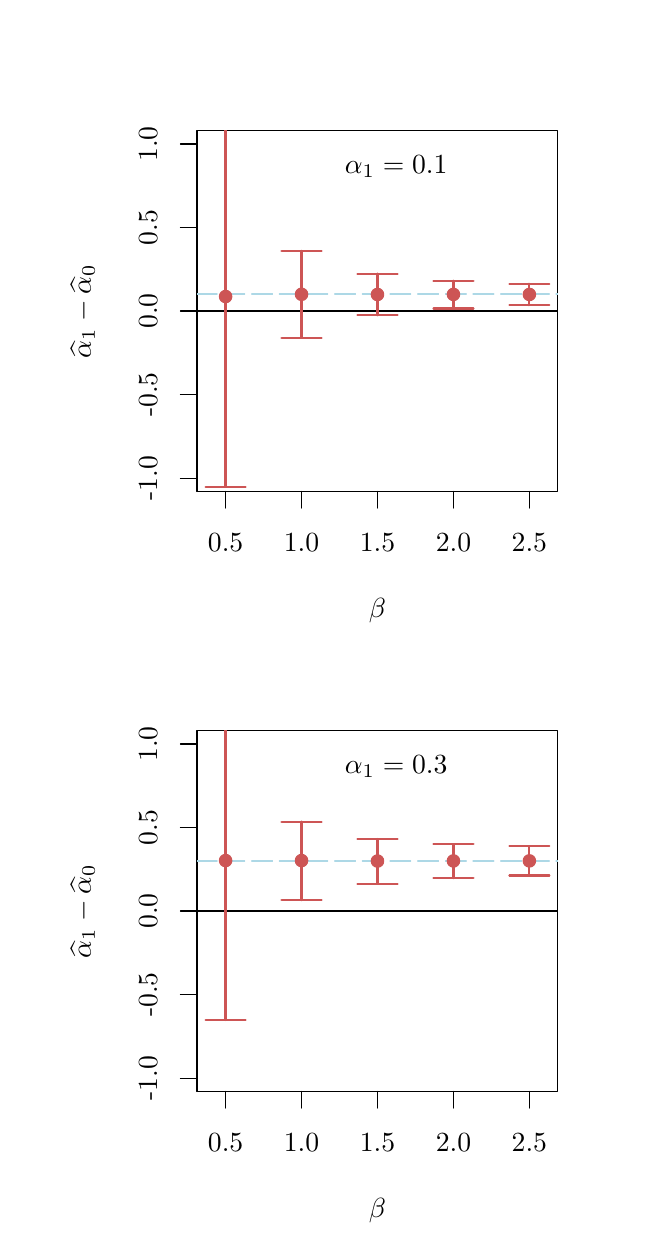
\begin{tikzpicture}[x=1pt,y=1pt]
\definecolor{fillColor}{RGB}{255,255,255}
\path[use as bounding box,fill=fillColor,fill opacity=0.00] (0,0) rectangle (216.81,433.62);
\begin{scope}
\path[clip] ( 61.20,266.01) rectangle (191.61,396.42);
\definecolor{drawColor}{RGB}{255,255,255}
\definecolor{fillColor}{RGB}{255,255,255}

\path[draw=drawColor,line width= 0.4pt,line join=round,line cap=round,fill=fillColor] ( 71.52,336.46) circle (  2.25);

\path[draw=drawColor,line width= 0.4pt,line join=round,line cap=round,fill=fillColor] ( 98.96,337.27) circle (  2.25);

\path[draw=drawColor,line width= 0.4pt,line join=round,line cap=round,fill=fillColor] (126.40,337.20) circle (  2.25);

\path[draw=drawColor,line width= 0.4pt,line join=round,line cap=round,fill=fillColor] (153.85,337.23) circle (  2.25);

\path[draw=drawColor,line width= 0.4pt,line join=round,line cap=round,fill=fillColor] (181.29,337.22) circle (  2.25);
\end{scope}
\begin{scope}
\path[clip] (  0.00,  0.00) rectangle (216.81,433.62);
\definecolor{drawColor}{RGB}{0,0,0}

\path[draw=drawColor,line width= 0.4pt,line join=round,line cap=round] ( 71.52,266.01) -- (181.29,266.01);

\path[draw=drawColor,line width= 0.4pt,line join=round,line cap=round] ( 71.52,266.01) -- ( 71.52,260.01);

\path[draw=drawColor,line width= 0.4pt,line join=round,line cap=round] ( 98.96,266.01) -- ( 98.96,260.01);

\path[draw=drawColor,line width= 0.4pt,line join=round,line cap=round] (126.40,266.01) -- (126.40,260.01);

\path[draw=drawColor,line width= 0.4pt,line join=round,line cap=round] (153.85,266.01) -- (153.85,260.01);

\path[draw=drawColor,line width= 0.4pt,line join=round,line cap=round] (181.29,266.01) -- (181.29,260.01);

\node[text=drawColor,anchor=base,inner sep=0pt, outer sep=0pt, scale=  1.00] at ( 71.52,244.41) {0.5};

\node[text=drawColor,anchor=base,inner sep=0pt, outer sep=0pt, scale=  1.00] at ( 98.96,244.41) {1.0};

\node[text=drawColor,anchor=base,inner sep=0pt, outer sep=0pt, scale=  1.00] at (126.40,244.41) {1.5};

\node[text=drawColor,anchor=base,inner sep=0pt, outer sep=0pt, scale=  1.00] at (153.85,244.41) {2.0};

\node[text=drawColor,anchor=base,inner sep=0pt, outer sep=0pt, scale=  1.00] at (181.29,244.41) {2.5};

\path[draw=drawColor,line width= 0.4pt,line join=round,line cap=round] ( 61.20,270.84) -- ( 61.20,391.59);

\path[draw=drawColor,line width= 0.4pt,line join=round,line cap=round] ( 61.20,270.84) -- ( 55.20,270.84);

\path[draw=drawColor,line width= 0.4pt,line join=round,line cap=round] ( 61.20,301.03) -- ( 55.20,301.03);

\path[draw=drawColor,line width= 0.4pt,line join=round,line cap=round] ( 61.20,331.22) -- ( 55.20,331.22);

\path[draw=drawColor,line width= 0.4pt,line join=round,line cap=round] ( 61.20,361.40) -- ( 55.20,361.40);

\path[draw=drawColor,line width= 0.4pt,line join=round,line cap=round] ( 61.20,391.59) -- ( 55.20,391.59);

\node[text=drawColor,rotate= 90.00,anchor=base,inner sep=0pt, outer sep=0pt, scale=  1.00] at ( 46.80,270.84) {-1.0};

\node[text=drawColor,rotate= 90.00,anchor=base,inner sep=0pt, outer sep=0pt, scale=  1.00] at ( 46.80,301.03) {-0.5};

\node[text=drawColor,rotate= 90.00,anchor=base,inner sep=0pt, outer sep=0pt, scale=  1.00] at ( 46.80,331.22) {0.0};

\node[text=drawColor,rotate= 90.00,anchor=base,inner sep=0pt, outer sep=0pt, scale=  1.00] at ( 46.80,361.40) {0.5};

\node[text=drawColor,rotate= 90.00,anchor=base,inner sep=0pt, outer sep=0pt, scale=  1.00] at ( 46.80,391.59) {1.0};

\path[draw=drawColor,line width= 0.4pt,line join=round,line cap=round] ( 61.20,266.01) --
	(191.61,266.01) --
	(191.61,396.42) --
	( 61.20,396.42) --
	( 61.20,266.01);
\end{scope}
\begin{scope}
\path[clip] (  0.00,216.81) rectangle (216.81,433.62);
\definecolor{drawColor}{RGB}{0,0,0}

\node[text=drawColor,anchor=base,inner sep=0pt, outer sep=0pt, scale=  1.00] at (126.41,220.41) {$\beta$};

\node[text=drawColor,rotate= 90.00,anchor=base,inner sep=0pt, outer sep=0pt, scale=  1.00] at ( 22.80,331.22) {$\widehat{\alpha}_1 - \widehat{\alpha}_0$};
\end{scope}
\begin{scope}
\path[clip] ( 61.20,266.01) rectangle (191.61,396.42);
\definecolor{drawColor}{RGB}{0,0,0}

\node[text=drawColor,anchor=base west,inner sep=0pt, outer sep=0pt, scale=  1.00] at (114.66,380.98) {$\alpha_1=0.1$};
\definecolor{drawColor}{RGB}{173,216,230}

\path[draw=drawColor,line width= 0.8pt,dash pattern=on 7pt off 3pt ,line join=round,line cap=round] ( 61.20,337.25) -- (191.61,337.25);

\path[draw=drawColor,line width= 0.8pt,dash pattern=on 7pt off 3pt ,line join=round,line cap=round] ( 61.20,337.25) -- (191.61,337.25);

\path[draw=drawColor,line width= 0.8pt,dash pattern=on 7pt off 3pt ,line join=round,line cap=round] ( 61.20,337.25) -- (191.61,337.25);

\path[draw=drawColor,line width= 0.8pt,dash pattern=on 7pt off 3pt ,line join=round,line cap=round] ( 61.20,337.25) -- (191.61,337.25);

\path[draw=drawColor,line width= 0.8pt,dash pattern=on 7pt off 3pt ,line join=round,line cap=round] ( 61.20,337.25) -- (191.61,337.25);
\definecolor{drawColor}{RGB}{0,0,0}

\path[draw=drawColor,line width= 0.4pt,line join=round,line cap=round] ( 61.20,331.22) -- (191.61,331.22);
\definecolor{drawColor}{RGB}{205,85,85}

\path[draw=drawColor,line width= 0.8pt,line join=round,line cap=round] ( 71.52,267.69) -- ( 71.52,406.45);

\path[draw=drawColor,line width= 0.8pt,line join=round,line cap=round] ( 64.29,267.69) --
	( 71.52,267.69) --
	( 78.75,267.69);

\path[draw=drawColor,line width= 0.8pt,line join=round,line cap=round] ( 78.75,406.45) --
	( 71.52,406.45) --
	( 64.29,406.45);

\path[draw=drawColor,line width= 0.8pt,line join=round,line cap=round] ( 98.96,321.52) -- ( 98.96,352.95);

\path[draw=drawColor,line width= 0.8pt,line join=round,line cap=round] ( 91.73,321.52) --
	( 98.96,321.52) --
	(106.19,321.52);

\path[draw=drawColor,line width= 0.8pt,line join=round,line cap=round] (106.19,352.95) --
	( 98.96,352.95) --
	( 91.73,352.95);

\path[draw=drawColor,line width= 0.8pt,line join=round,line cap=round] (126.40,329.69) -- (126.40,344.74);

\path[draw=drawColor,line width= 0.8pt,line join=round,line cap=round] (119.18,329.69) --
	(126.40,329.69) --
	(133.63,329.69);

\path[draw=drawColor,line width= 0.8pt,line join=round,line cap=round] (133.63,344.74) --
	(126.40,344.74) --
	(119.18,344.74);

\path[draw=drawColor,line width= 0.8pt,line join=round,line cap=round] (153.85,332.12) -- (153.85,342.17);

\path[draw=drawColor,line width= 0.8pt,line join=round,line cap=round] (146.62,332.12) --
	(153.85,332.12) --
	(161.08,332.12);

\path[draw=drawColor,line width= 0.8pt,line join=round,line cap=round] (161.08,342.17) --
	(153.85,342.17) --
	(146.62,342.17);

\path[draw=drawColor,line width= 0.8pt,line join=round,line cap=round] (181.29,333.34) -- (181.29,341.06);

\path[draw=drawColor,line width= 0.8pt,line join=round,line cap=round] (174.06,333.34) --
	(181.29,333.34) --
	(188.52,333.34);

\path[draw=drawColor,line width= 0.8pt,line join=round,line cap=round] (188.52,341.06) --
	(181.29,341.06) --
	(174.06,341.06);
\definecolor{fillColor}{RGB}{205,85,85}

\path[draw=drawColor,line width= 0.4pt,line join=round,line cap=round,fill=fillColor] ( 71.52,336.46) circle (  2.25);

\path[draw=drawColor,line width= 0.4pt,line join=round,line cap=round,fill=fillColor] ( 98.96,337.27) circle (  2.25);

\path[draw=drawColor,line width= 0.4pt,line join=round,line cap=round,fill=fillColor] (126.40,337.20) circle (  2.25);

\path[draw=drawColor,line width= 0.4pt,line join=round,line cap=round,fill=fillColor] (153.85,337.23) circle (  2.25);

\path[draw=drawColor,line width= 0.4pt,line join=round,line cap=round,fill=fillColor] (181.29,337.22) circle (  2.25);
\end{scope}
\begin{scope}
\path[clip] ( 61.20, 49.20) rectangle (191.61,179.61);
\definecolor{drawColor}{RGB}{255,255,255}
\definecolor{fillColor}{RGB}{255,255,255}

\path[draw=drawColor,line width= 0.4pt,line join=round,line cap=round,fill=fillColor] ( 71.52,132.65) circle (  2.25);

\path[draw=drawColor,line width= 0.4pt,line join=round,line cap=round,fill=fillColor] ( 98.96,132.65) circle (  2.25);

\path[draw=drawColor,line width= 0.4pt,line join=round,line cap=round,fill=fillColor] (126.40,132.48) circle (  2.25);

\path[draw=drawColor,line width= 0.4pt,line join=round,line cap=round,fill=fillColor] (153.85,132.52) circle (  2.25);

\path[draw=drawColor,line width= 0.4pt,line join=round,line cap=round,fill=fillColor] (181.29,132.54) circle (  2.25);
\end{scope}
\begin{scope}
\path[clip] (  0.00,  0.00) rectangle (216.81,433.62);
\definecolor{drawColor}{RGB}{0,0,0}

\path[draw=drawColor,line width= 0.4pt,line join=round,line cap=round] ( 71.52, 49.20) -- (181.29, 49.20);

\path[draw=drawColor,line width= 0.4pt,line join=round,line cap=round] ( 71.52, 49.20) -- ( 71.52, 43.20);

\path[draw=drawColor,line width= 0.4pt,line join=round,line cap=round] ( 98.96, 49.20) -- ( 98.96, 43.20);

\path[draw=drawColor,line width= 0.4pt,line join=round,line cap=round] (126.40, 49.20) -- (126.40, 43.20);

\path[draw=drawColor,line width= 0.4pt,line join=round,line cap=round] (153.85, 49.20) -- (153.85, 43.20);

\path[draw=drawColor,line width= 0.4pt,line join=round,line cap=round] (181.29, 49.20) -- (181.29, 43.20);

\node[text=drawColor,anchor=base,inner sep=0pt, outer sep=0pt, scale=  1.00] at ( 71.52, 27.60) {0.5};

\node[text=drawColor,anchor=base,inner sep=0pt, outer sep=0pt, scale=  1.00] at ( 98.96, 27.60) {1.0};

\node[text=drawColor,anchor=base,inner sep=0pt, outer sep=0pt, scale=  1.00] at (126.40, 27.60) {1.5};

\node[text=drawColor,anchor=base,inner sep=0pt, outer sep=0pt, scale=  1.00] at (153.85, 27.60) {2.0};

\node[text=drawColor,anchor=base,inner sep=0pt, outer sep=0pt, scale=  1.00] at (181.29, 27.60) {2.5};

\path[draw=drawColor,line width= 0.4pt,line join=round,line cap=round] ( 61.20, 54.03) -- ( 61.20,174.78);

\path[draw=drawColor,line width= 0.4pt,line join=round,line cap=round] ( 61.20, 54.03) -- ( 55.20, 54.03);

\path[draw=drawColor,line width= 0.4pt,line join=round,line cap=round] ( 61.20, 84.22) -- ( 55.20, 84.22);

\path[draw=drawColor,line width= 0.4pt,line join=round,line cap=round] ( 61.20,114.41) -- ( 55.20,114.41);

\path[draw=drawColor,line width= 0.4pt,line join=round,line cap=round] ( 61.20,144.59) -- ( 55.20,144.59);

\path[draw=drawColor,line width= 0.4pt,line join=round,line cap=round] ( 61.20,174.78) -- ( 55.20,174.78);

\node[text=drawColor,rotate= 90.00,anchor=base,inner sep=0pt, outer sep=0pt, scale=  1.00] at ( 46.80, 54.03) {-1.0};

\node[text=drawColor,rotate= 90.00,anchor=base,inner sep=0pt, outer sep=0pt, scale=  1.00] at ( 46.80, 84.22) {-0.5};

\node[text=drawColor,rotate= 90.00,anchor=base,inner sep=0pt, outer sep=0pt, scale=  1.00] at ( 46.80,114.41) {0.0};

\node[text=drawColor,rotate= 90.00,anchor=base,inner sep=0pt, outer sep=0pt, scale=  1.00] at ( 46.80,144.59) {0.5};

\node[text=drawColor,rotate= 90.00,anchor=base,inner sep=0pt, outer sep=0pt, scale=  1.00] at ( 46.80,174.78) {1.0};

\path[draw=drawColor,line width= 0.4pt,line join=round,line cap=round] ( 61.20, 49.20) --
	(191.61, 49.20) --
	(191.61,179.61) --
	( 61.20,179.61) --
	( 61.20, 49.20);
\end{scope}
\begin{scope}
\path[clip] (  0.00,  0.00) rectangle (216.81,216.81);
\definecolor{drawColor}{RGB}{0,0,0}

\node[text=drawColor,anchor=base,inner sep=0pt, outer sep=0pt, scale=  1.00] at (126.41,  3.60) {$\beta$};

\node[text=drawColor,rotate= 90.00,anchor=base,inner sep=0pt, outer sep=0pt, scale=  1.00] at ( 22.80,114.41) {$\widehat{\alpha}_1 - \widehat{\alpha}_0$};
\end{scope}
\begin{scope}
\path[clip] ( 61.20, 49.20) rectangle (191.61,179.61);
\definecolor{drawColor}{RGB}{0,0,0}

\node[text=drawColor,anchor=base west,inner sep=0pt, outer sep=0pt, scale=  1.00] at (114.66,164.17) {$\alpha_1=0.3$};
\definecolor{drawColor}{RGB}{173,216,230}

\path[draw=drawColor,line width= 0.8pt,dash pattern=on 7pt off 3pt ,line join=round,line cap=round] ( 61.20,132.52) -- (191.61,132.52);

\path[draw=drawColor,line width= 0.8pt,dash pattern=on 7pt off 3pt ,line join=round,line cap=round] ( 61.20,132.52) -- (191.61,132.52);

\path[draw=drawColor,line width= 0.8pt,dash pattern=on 7pt off 3pt ,line join=round,line cap=round] ( 61.20,132.52) -- (191.61,132.52);

\path[draw=drawColor,line width= 0.8pt,dash pattern=on 7pt off 3pt ,line join=round,line cap=round] ( 61.20,132.52) -- (191.61,132.52);

\path[draw=drawColor,line width= 0.8pt,dash pattern=on 7pt off 3pt ,line join=round,line cap=round] ( 61.20,132.52) -- (191.61,132.52);
\definecolor{drawColor}{RGB}{0,0,0}

\path[draw=drawColor,line width= 0.4pt,line join=round,line cap=round] ( 61.20,114.41) -- (191.61,114.41);
\definecolor{drawColor}{RGB}{205,85,85}

\path[draw=drawColor,line width= 0.8pt,line join=round,line cap=round] ( 71.52, 75.06) -- ( 71.52,186.72);

\path[draw=drawColor,line width= 0.8pt,line join=round,line cap=round] ( 64.29, 75.06) --
	( 71.52, 75.06) --
	( 78.75, 75.06);

\path[draw=drawColor,line width= 0.8pt,line join=round,line cap=round] ( 78.75,186.72) --
	( 71.52,186.72) --
	( 64.29,186.72);

\path[draw=drawColor,line width= 0.8pt,line join=round,line cap=round] ( 98.96,118.37) -- ( 98.96,146.71);

\path[draw=drawColor,line width= 0.8pt,line join=round,line cap=round] ( 91.73,118.37) --
	( 98.96,118.37) --
	(106.19,118.37);

\path[draw=drawColor,line width= 0.8pt,line join=round,line cap=round] (106.19,146.71) --
	( 98.96,146.71) --
	( 91.73,146.71);

\path[draw=drawColor,line width= 0.8pt,line join=round,line cap=round] (126.40,124.32) -- (126.40,140.45);

\path[draw=drawColor,line width= 0.8pt,line join=round,line cap=round] (119.18,124.32) --
	(126.40,124.32) --
	(133.63,124.32);

\path[draw=drawColor,line width= 0.8pt,line join=round,line cap=round] (133.63,140.45) --
	(126.40,140.45) --
	(119.18,140.45);

\path[draw=drawColor,line width= 0.8pt,line join=round,line cap=round] (153.85,126.32) -- (153.85,138.58);

\path[draw=drawColor,line width= 0.8pt,line join=round,line cap=round] (146.62,126.32) --
	(153.85,126.32) --
	(161.08,126.32);

\path[draw=drawColor,line width= 0.8pt,line join=round,line cap=round] (161.08,138.58) --
	(153.85,138.58) --
	(146.62,138.58);

\path[draw=drawColor,line width= 0.8pt,line join=round,line cap=round] (181.29,127.29) -- (181.29,137.80);

\path[draw=drawColor,line width= 0.8pt,line join=round,line cap=round] (174.06,127.29) --
	(181.29,127.29) --
	(188.52,127.29);

\path[draw=drawColor,line width= 0.8pt,line join=round,line cap=round] (188.52,137.80) --
	(181.29,137.80) --
	(174.06,137.80);
\definecolor{fillColor}{RGB}{205,85,85}

\path[draw=drawColor,line width= 0.4pt,line join=round,line cap=round,fill=fillColor] ( 71.52,132.65) circle (  2.25);

\path[draw=drawColor,line width= 0.4pt,line join=round,line cap=round,fill=fillColor] ( 98.96,132.65) circle (  2.25);

\path[draw=drawColor,line width= 0.4pt,line join=round,line cap=round,fill=fillColor] (126.40,132.48) circle (  2.25);

\path[draw=drawColor,line width= 0.4pt,line join=round,line cap=round,fill=fillColor] (153.85,132.52) circle (  2.25);

\path[draw=drawColor,line width= 0.4pt,line join=round,line cap=round,fill=fillColor] (181.29,132.54) circle (  2.25);
\end{scope}
\end{tikzpicture}

%  \end{subfigure}
%  ~
%  \begin{subfigure}[b]{0.31\textwidth}
%\caption{\footnotesize $N=5000, \delta = 0.2$}
%  % Created by tikzDevice version 0.8.1 on 2015-11-17 11:43:48
% !TEX encoding = UTF-8 Unicode
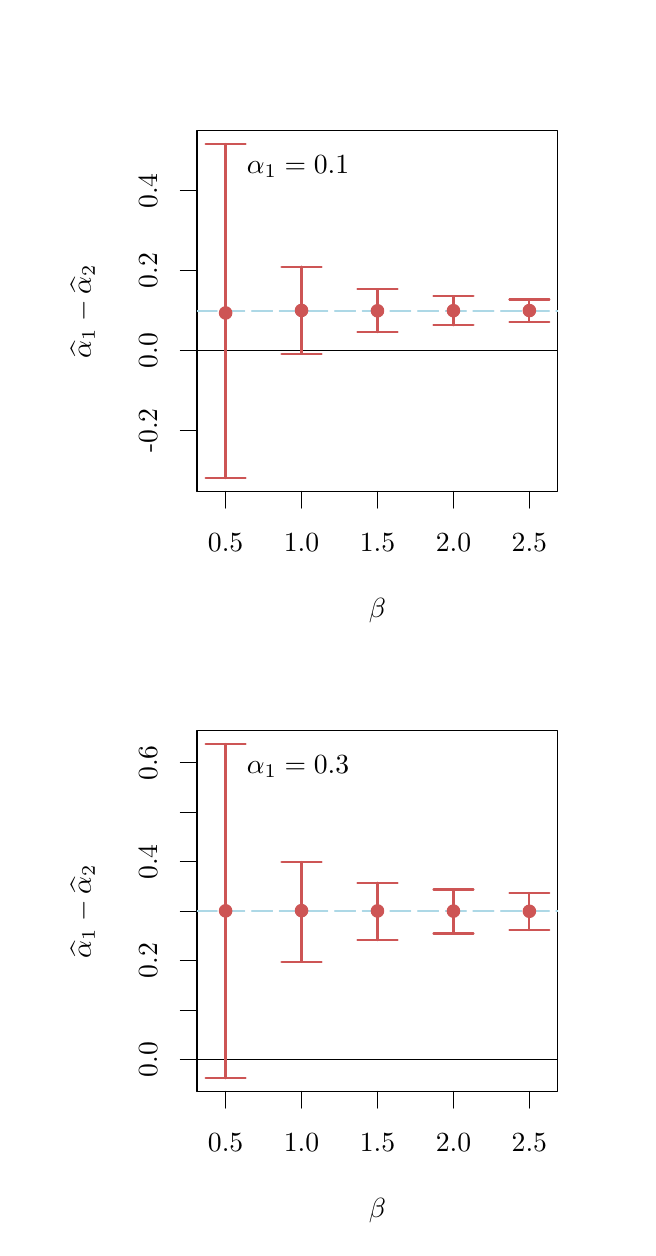
\begin{tikzpicture}[x=1pt,y=1pt]
\definecolor{fillColor}{RGB}{255,255,255}
\path[use as bounding box,fill=fillColor,fill opacity=0.00] (0,0) rectangle (216.81,433.62);
\begin{scope}
\path[clip] ( 61.20,266.01) rectangle (191.61,396.42);
\definecolor{drawColor}{RGB}{255,255,255}
\definecolor{fillColor}{RGB}{255,255,255}

\path[draw=drawColor,line width= 0.4pt,line join=round,line cap=round,fill=fillColor] ( 71.52,330.53) circle (  2.25);

\path[draw=drawColor,line width= 0.4pt,line join=round,line cap=round,fill=fillColor] ( 98.96,331.44) circle (  2.25);

\path[draw=drawColor,line width= 0.4pt,line join=round,line cap=round,fill=fillColor] (126.40,331.31) circle (  2.25);

\path[draw=drawColor,line width= 0.4pt,line join=round,line cap=round,fill=fillColor] (153.85,331.35) circle (  2.25);

\path[draw=drawColor,line width= 0.4pt,line join=round,line cap=round,fill=fillColor] (181.29,331.39) circle (  2.25);
\end{scope}
\begin{scope}
\path[clip] (  0.00,  0.00) rectangle (216.81,433.62);
\definecolor{drawColor}{RGB}{0,0,0}

\path[draw=drawColor,line width= 0.4pt,line join=round,line cap=round] ( 71.52,266.01) -- (181.29,266.01);

\path[draw=drawColor,line width= 0.4pt,line join=round,line cap=round] ( 71.52,266.01) -- ( 71.52,260.01);

\path[draw=drawColor,line width= 0.4pt,line join=round,line cap=round] ( 98.96,266.01) -- ( 98.96,260.01);

\path[draw=drawColor,line width= 0.4pt,line join=round,line cap=round] (126.40,266.01) -- (126.40,260.01);

\path[draw=drawColor,line width= 0.4pt,line join=round,line cap=round] (153.85,266.01) -- (153.85,260.01);

\path[draw=drawColor,line width= 0.4pt,line join=round,line cap=round] (181.29,266.01) -- (181.29,260.01);

\node[text=drawColor,anchor=base,inner sep=0pt, outer sep=0pt, scale=  1.00] at ( 71.52,244.41) {0.5};

\node[text=drawColor,anchor=base,inner sep=0pt, outer sep=0pt, scale=  1.00] at ( 98.96,244.41) {1.0};

\node[text=drawColor,anchor=base,inner sep=0pt, outer sep=0pt, scale=  1.00] at (126.40,244.41) {1.5};

\node[text=drawColor,anchor=base,inner sep=0pt, outer sep=0pt, scale=  1.00] at (153.85,244.41) {2.0};

\node[text=drawColor,anchor=base,inner sep=0pt, outer sep=0pt, scale=  1.00] at (181.29,244.41) {2.5};

\path[draw=drawColor,line width= 0.4pt,line join=round,line cap=round] ( 61.20,288.03) -- ( 61.20,374.63);

\path[draw=drawColor,line width= 0.4pt,line join=round,line cap=round] ( 61.20,288.03) -- ( 55.20,288.03);

\path[draw=drawColor,line width= 0.4pt,line join=round,line cap=round] ( 61.20,316.90) -- ( 55.20,316.90);

\path[draw=drawColor,line width= 0.4pt,line join=round,line cap=round] ( 61.20,345.76) -- ( 55.20,345.76);

\path[draw=drawColor,line width= 0.4pt,line join=round,line cap=round] ( 61.20,374.63) -- ( 55.20,374.63);

\node[text=drawColor,rotate= 90.00,anchor=base,inner sep=0pt, outer sep=0pt, scale=  1.00] at ( 46.80,288.03) {-0.2};

\node[text=drawColor,rotate= 90.00,anchor=base,inner sep=0pt, outer sep=0pt, scale=  1.00] at ( 46.80,316.90) {0.0};

\node[text=drawColor,rotate= 90.00,anchor=base,inner sep=0pt, outer sep=0pt, scale=  1.00] at ( 46.80,345.76) {0.2};

\node[text=drawColor,rotate= 90.00,anchor=base,inner sep=0pt, outer sep=0pt, scale=  1.00] at ( 46.80,374.63) {0.4};

\path[draw=drawColor,line width= 0.4pt,line join=round,line cap=round] ( 61.20,266.01) --
	(191.61,266.01) --
	(191.61,396.42) --
	( 61.20,396.42) --
	( 61.20,266.01);
\end{scope}
\begin{scope}
\path[clip] (  0.00,216.81) rectangle (216.81,433.62);
\definecolor{drawColor}{RGB}{0,0,0}

\node[text=drawColor,anchor=base,inner sep=0pt, outer sep=0pt, scale=  1.00] at (126.41,220.41) {$\beta$};

\node[text=drawColor,rotate= 90.00,anchor=base,inner sep=0pt, outer sep=0pt, scale=  1.00] at ( 22.80,331.22) {$\widehat{\alpha}_1 - \widehat{\alpha}_2$};
\end{scope}
\begin{scope}
\path[clip] ( 61.20,266.01) rectangle (191.61,396.42);
\definecolor{drawColor}{RGB}{0,0,0}

\node[text=drawColor,anchor=base west,inner sep=0pt, outer sep=0pt, scale=  1.00] at ( 79.20,380.98) {$\alpha_1=0.1$};
\definecolor{drawColor}{RGB}{173,216,230}

\path[draw=drawColor,line width= 0.8pt,dash pattern=on 7pt off 3pt ,line join=round,line cap=round] ( 61.20,331.33) -- (191.61,331.33);

\path[draw=drawColor,line width= 0.8pt,dash pattern=on 7pt off 3pt ,line join=round,line cap=round] ( 61.20,331.33) -- (191.61,331.33);

\path[draw=drawColor,line width= 0.8pt,dash pattern=on 7pt off 3pt ,line join=round,line cap=round] ( 61.20,331.33) -- (191.61,331.33);

\path[draw=drawColor,line width= 0.8pt,dash pattern=on 7pt off 3pt ,line join=round,line cap=round] ( 61.20,331.33) -- (191.61,331.33);

\path[draw=drawColor,line width= 0.8pt,dash pattern=on 7pt off 3pt ,line join=round,line cap=round] ( 61.20,331.33) -- (191.61,331.33);
\definecolor{drawColor}{RGB}{0,0,0}

\path[draw=drawColor,line width= 0.4pt,line join=round,line cap=round] ( 61.20,316.90) -- (191.61,316.90);
\definecolor{drawColor}{RGB}{205,85,85}

\path[draw=drawColor,line width= 0.8pt,line join=round,line cap=round] ( 71.52,270.84) -- ( 71.52,391.59);

\path[draw=drawColor,line width= 0.8pt,line join=round,line cap=round] ( 64.29,270.84) --
	( 71.52,270.84) --
	( 78.75,270.84);

\path[draw=drawColor,line width= 0.8pt,line join=round,line cap=round] ( 78.75,391.59) --
	( 71.52,391.59) --
	( 64.29,391.59);

\path[draw=drawColor,line width= 0.8pt,line join=round,line cap=round] ( 98.96,315.80) -- ( 98.96,347.26);

\path[draw=drawColor,line width= 0.8pt,line join=round,line cap=round] ( 91.73,315.80) --
	( 98.96,315.80) --
	(106.19,315.80);

\path[draw=drawColor,line width= 0.8pt,line join=round,line cap=round] (106.19,347.26) --
	( 98.96,347.26) --
	( 91.73,347.26);

\path[draw=drawColor,line width= 0.8pt,line join=round,line cap=round] (126.40,323.61) -- (126.40,339.05);

\path[draw=drawColor,line width= 0.8pt,line join=round,line cap=round] (119.18,323.61) --
	(126.40,323.61) --
	(133.63,323.61);

\path[draw=drawColor,line width= 0.8pt,line join=round,line cap=round] (133.63,339.05) --
	(126.40,339.05) --
	(119.18,339.05);

\path[draw=drawColor,line width= 0.8pt,line join=round,line cap=round] (153.85,326.06) -- (153.85,336.57);

\path[draw=drawColor,line width= 0.8pt,line join=round,line cap=round] (146.62,326.06) --
	(153.85,326.06) --
	(161.08,326.06);

\path[draw=drawColor,line width= 0.8pt,line join=round,line cap=round] (161.08,336.57) --
	(153.85,336.57) --
	(146.62,336.57);

\path[draw=drawColor,line width= 0.8pt,line join=round,line cap=round] (181.29,327.32) -- (181.29,335.40);

\path[draw=drawColor,line width= 0.8pt,line join=round,line cap=round] (174.06,327.32) --
	(181.29,327.32) --
	(188.52,327.32);

\path[draw=drawColor,line width= 0.8pt,line join=round,line cap=round] (188.52,335.40) --
	(181.29,335.40) --
	(174.06,335.40);
\definecolor{fillColor}{RGB}{205,85,85}

\path[draw=drawColor,line width= 0.4pt,line join=round,line cap=round,fill=fillColor] ( 71.52,330.53) circle (  2.25);

\path[draw=drawColor,line width= 0.4pt,line join=round,line cap=round,fill=fillColor] ( 98.96,331.44) circle (  2.25);

\path[draw=drawColor,line width= 0.4pt,line join=round,line cap=round,fill=fillColor] (126.40,331.31) circle (  2.25);

\path[draw=drawColor,line width= 0.4pt,line join=round,line cap=round,fill=fillColor] (153.85,331.35) circle (  2.25);

\path[draw=drawColor,line width= 0.4pt,line join=round,line cap=round,fill=fillColor] (181.29,331.39) circle (  2.25);
\end{scope}
\begin{scope}
\path[clip] ( 61.20, 49.20) rectangle (191.61,179.61);
\definecolor{drawColor}{RGB}{255,255,255}
\definecolor{fillColor}{RGB}{255,255,255}

\path[draw=drawColor,line width= 0.4pt,line join=round,line cap=round,fill=fillColor] ( 71.52,114.48) circle (  2.25);

\path[draw=drawColor,line width= 0.4pt,line join=round,line cap=round,fill=fillColor] ( 98.96,114.56) circle (  2.25);

\path[draw=drawColor,line width= 0.4pt,line join=round,line cap=round,fill=fillColor] (126.40,114.45) circle (  2.25);

\path[draw=drawColor,line width= 0.4pt,line join=round,line cap=round,fill=fillColor] (153.85,114.39) circle (  2.25);

\path[draw=drawColor,line width= 0.4pt,line join=round,line cap=round,fill=fillColor] (181.29,114.33) circle (  2.25);
\end{scope}
\begin{scope}
\path[clip] (  0.00,  0.00) rectangle (216.81,433.62);
\definecolor{drawColor}{RGB}{0,0,0}

\path[draw=drawColor,line width= 0.4pt,line join=round,line cap=round] ( 71.52, 49.20) -- (181.29, 49.20);

\path[draw=drawColor,line width= 0.4pt,line join=round,line cap=round] ( 71.52, 49.20) -- ( 71.52, 43.20);

\path[draw=drawColor,line width= 0.4pt,line join=round,line cap=round] ( 98.96, 49.20) -- ( 98.96, 43.20);

\path[draw=drawColor,line width= 0.4pt,line join=round,line cap=round] (126.40, 49.20) -- (126.40, 43.20);

\path[draw=drawColor,line width= 0.4pt,line join=round,line cap=round] (153.85, 49.20) -- (153.85, 43.20);

\path[draw=drawColor,line width= 0.4pt,line join=round,line cap=round] (181.29, 49.20) -- (181.29, 43.20);

\node[text=drawColor,anchor=base,inner sep=0pt, outer sep=0pt, scale=  1.00] at ( 71.52, 27.60) {0.5};

\node[text=drawColor,anchor=base,inner sep=0pt, outer sep=0pt, scale=  1.00] at ( 98.96, 27.60) {1.0};

\node[text=drawColor,anchor=base,inner sep=0pt, outer sep=0pt, scale=  1.00] at (126.40, 27.60) {1.5};

\node[text=drawColor,anchor=base,inner sep=0pt, outer sep=0pt, scale=  1.00] at (153.85, 27.60) {2.0};

\node[text=drawColor,anchor=base,inner sep=0pt, outer sep=0pt, scale=  1.00] at (181.29, 27.60) {2.5};

\path[draw=drawColor,line width= 0.4pt,line join=round,line cap=round] ( 61.20, 60.72) -- ( 61.20,167.93);

\path[draw=drawColor,line width= 0.4pt,line join=round,line cap=round] ( 61.20, 60.72) -- ( 55.20, 60.72);

\path[draw=drawColor,line width= 0.4pt,line join=round,line cap=round] ( 61.20, 78.59) -- ( 55.20, 78.59);

\path[draw=drawColor,line width= 0.4pt,line join=round,line cap=round] ( 61.20, 96.45) -- ( 55.20, 96.45);

\path[draw=drawColor,line width= 0.4pt,line join=round,line cap=round] ( 61.20,114.32) -- ( 55.20,114.32);

\path[draw=drawColor,line width= 0.4pt,line join=round,line cap=round] ( 61.20,132.19) -- ( 55.20,132.19);

\path[draw=drawColor,line width= 0.4pt,line join=round,line cap=round] ( 61.20,150.06) -- ( 55.20,150.06);

\path[draw=drawColor,line width= 0.4pt,line join=round,line cap=round] ( 61.20,167.93) -- ( 55.20,167.93);

\node[text=drawColor,rotate= 90.00,anchor=base,inner sep=0pt, outer sep=0pt, scale=  1.00] at ( 46.80, 60.72) {0.0};

\node[text=drawColor,rotate= 90.00,anchor=base,inner sep=0pt, outer sep=0pt, scale=  1.00] at ( 46.80, 96.45) {0.2};

\node[text=drawColor,rotate= 90.00,anchor=base,inner sep=0pt, outer sep=0pt, scale=  1.00] at ( 46.80,132.19) {0.4};

\node[text=drawColor,rotate= 90.00,anchor=base,inner sep=0pt, outer sep=0pt, scale=  1.00] at ( 46.80,167.93) {0.6};

\path[draw=drawColor,line width= 0.4pt,line join=round,line cap=round] ( 61.20, 49.20) --
	(191.61, 49.20) --
	(191.61,179.61) --
	( 61.20,179.61) --
	( 61.20, 49.20);
\end{scope}
\begin{scope}
\path[clip] (  0.00,  0.00) rectangle (216.81,216.81);
\definecolor{drawColor}{RGB}{0,0,0}

\node[text=drawColor,anchor=base,inner sep=0pt, outer sep=0pt, scale=  1.00] at (126.41,  3.60) {$\beta$};

\node[text=drawColor,rotate= 90.00,anchor=base,inner sep=0pt, outer sep=0pt, scale=  1.00] at ( 22.80,114.41) {$\widehat{\alpha}_1 - \widehat{\alpha}_2$};
\end{scope}
\begin{scope}
\path[clip] ( 61.20, 49.20) rectangle (191.61,179.61);
\definecolor{drawColor}{RGB}{0,0,0}

\node[text=drawColor,anchor=base west,inner sep=0pt, outer sep=0pt, scale=  1.00] at ( 79.20,164.17) {$\alpha_1=0.3$};
\definecolor{drawColor}{RGB}{173,216,230}

\path[draw=drawColor,line width= 0.8pt,dash pattern=on 7pt off 3pt ,line join=round,line cap=round] ( 61.20,114.32) -- (191.61,114.32);

\path[draw=drawColor,line width= 0.8pt,dash pattern=on 7pt off 3pt ,line join=round,line cap=round] ( 61.20,114.32) -- (191.61,114.32);

\path[draw=drawColor,line width= 0.8pt,dash pattern=on 7pt off 3pt ,line join=round,line cap=round] ( 61.20,114.32) -- (191.61,114.32);

\path[draw=drawColor,line width= 0.8pt,dash pattern=on 7pt off 3pt ,line join=round,line cap=round] ( 61.20,114.32) -- (191.61,114.32);

\path[draw=drawColor,line width= 0.8pt,dash pattern=on 7pt off 3pt ,line join=round,line cap=round] ( 61.20,114.32) -- (191.61,114.32);
\definecolor{drawColor}{RGB}{0,0,0}

\path[draw=drawColor,line width= 0.4pt,line join=round,line cap=round] ( 61.20, 60.72) -- (191.61, 60.72);
\definecolor{drawColor}{RGB}{205,85,85}

\path[draw=drawColor,line width= 0.8pt,line join=round,line cap=round] ( 71.52, 54.03) -- ( 71.52,174.78);

\path[draw=drawColor,line width= 0.8pt,line join=round,line cap=round] ( 64.29, 54.03) --
	( 71.52, 54.03) --
	( 78.75, 54.03);

\path[draw=drawColor,line width= 0.8pt,line join=round,line cap=round] ( 78.75,174.78) --
	( 71.52,174.78) --
	( 64.29,174.78);

\path[draw=drawColor,line width= 0.8pt,line join=round,line cap=round] ( 98.96, 96.05) -- ( 98.96,132.12);

\path[draw=drawColor,line width= 0.8pt,line join=round,line cap=round] ( 91.73, 96.05) --
	( 98.96, 96.05) --
	(106.19, 96.05);

\path[draw=drawColor,line width= 0.8pt,line join=round,line cap=round] (106.19,132.12) --
	( 98.96,132.12) --
	( 91.73,132.12);

\path[draw=drawColor,line width= 0.8pt,line join=round,line cap=round] (126.40,103.91) -- (126.40,124.64);

\path[draw=drawColor,line width= 0.8pt,line join=round,line cap=round] (119.18,103.91) --
	(126.40,103.91) --
	(133.63,103.91);

\path[draw=drawColor,line width= 0.8pt,line join=round,line cap=round] (133.63,124.64) --
	(126.40,124.64) --
	(119.18,124.64);

\path[draw=drawColor,line width= 0.8pt,line join=round,line cap=round] (153.85,106.30) -- (153.85,122.23);

\path[draw=drawColor,line width= 0.8pt,line join=round,line cap=round] (146.62,106.30) --
	(153.85,106.30) --
	(161.08,106.30);

\path[draw=drawColor,line width= 0.8pt,line join=round,line cap=round] (161.08,122.23) --
	(153.85,122.23) --
	(146.62,122.23);

\path[draw=drawColor,line width= 0.8pt,line join=round,line cap=round] (181.29,107.54) -- (181.29,120.91);

\path[draw=drawColor,line width= 0.8pt,line join=round,line cap=round] (174.06,107.54) --
	(181.29,107.54) --
	(188.52,107.54);

\path[draw=drawColor,line width= 0.8pt,line join=round,line cap=round] (188.52,120.91) --
	(181.29,120.91) --
	(174.06,120.91);
\definecolor{fillColor}{RGB}{205,85,85}

\path[draw=drawColor,line width= 0.4pt,line join=round,line cap=round,fill=fillColor] ( 71.52,114.48) circle (  2.25);

\path[draw=drawColor,line width= 0.4pt,line join=round,line cap=round,fill=fillColor] ( 98.96,114.56) circle (  2.25);

\path[draw=drawColor,line width= 0.4pt,line join=round,line cap=round,fill=fillColor] (126.40,114.45) circle (  2.25);

\path[draw=drawColor,line width= 0.4pt,line join=round,line cap=round,fill=fillColor] (153.85,114.39) circle (  2.25);

\path[draw=drawColor,line width= 0.4pt,line join=round,line cap=round,fill=fillColor] (181.29,114.33) circle (  2.25);
\end{scope}
\end{tikzpicture}

%  \end{subfigure}
%\endgroup
%\end{figure}
%\end{frame}
%%%%%%%%%%%%%%%%%%%%%%%%%%%%%%%%%%%%%%
%\begin{frame}
%\begin{figure}[h]
%  \scriptsize
%  \begingroup
%  \tikzset{every picture/.style={scale=0.53}}
%  \centering
%  \begin{subfigure}[b]{0.31\textwidth}
%\caption{\footnotesize $N=500, \delta = 0.3$}
%  % Created by tikzDevice version 0.8.1 on 2015-11-17 11:43:48
% !TEX encoding = UTF-8 Unicode
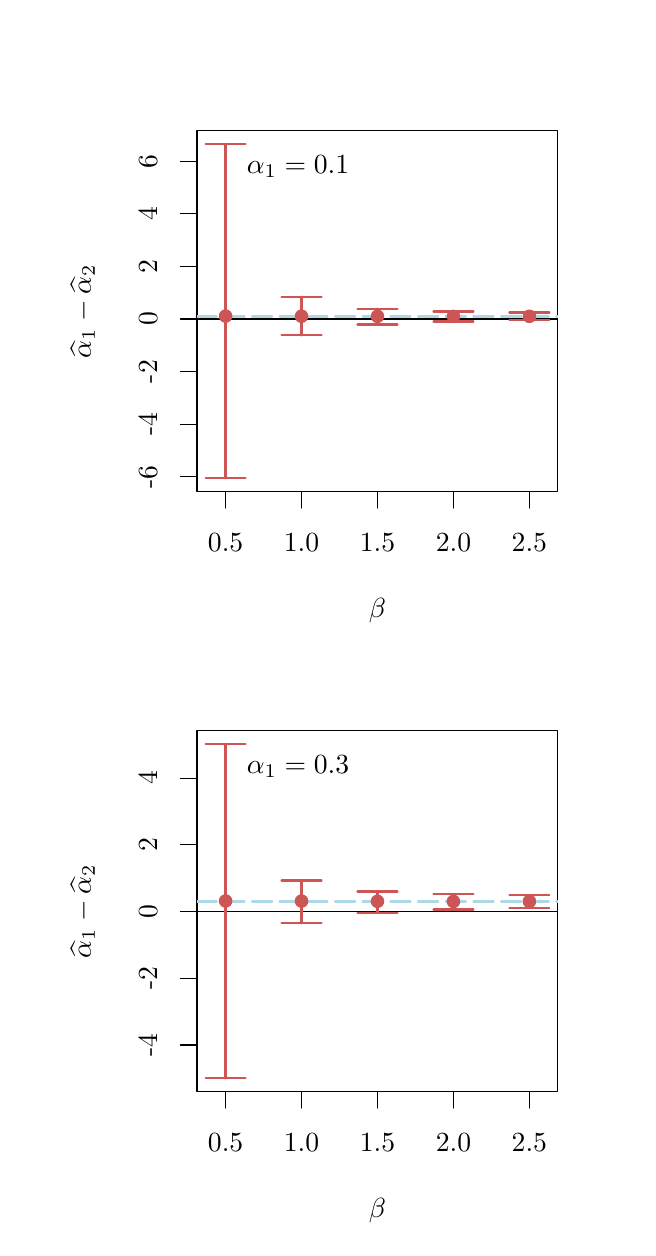
\begin{tikzpicture}[x=1pt,y=1pt]
\definecolor{fillColor}{RGB}{255,255,255}
\path[use as bounding box,fill=fillColor,fill opacity=0.00] (0,0) rectangle (216.81,433.62);
\begin{scope}
\path[clip] ( 61.20,266.01) rectangle (191.61,396.42);
\definecolor{drawColor}{RGB}{255,255,255}
\definecolor{fillColor}{RGB}{255,255,255}

\path[draw=drawColor,line width= 0.4pt,line join=round,line cap=round,fill=fillColor] ( 71.52,329.40) circle (  2.25);

\path[draw=drawColor,line width= 0.4pt,line join=round,line cap=round,fill=fillColor] ( 98.96,329.35) circle (  2.25);

\path[draw=drawColor,line width= 0.4pt,line join=round,line cap=round,fill=fillColor] (126.40,329.31) circle (  2.25);

\path[draw=drawColor,line width= 0.4pt,line join=round,line cap=round,fill=fillColor] (153.85,329.29) circle (  2.25);

\path[draw=drawColor,line width= 0.4pt,line join=round,line cap=round,fill=fillColor] (181.29,329.31) circle (  2.25);
\end{scope}
\begin{scope}
\path[clip] (  0.00,  0.00) rectangle (216.81,433.62);
\definecolor{drawColor}{RGB}{0,0,0}

\path[draw=drawColor,line width= 0.4pt,line join=round,line cap=round] ( 71.52,266.01) -- (181.29,266.01);

\path[draw=drawColor,line width= 0.4pt,line join=round,line cap=round] ( 71.52,266.01) -- ( 71.52,260.01);

\path[draw=drawColor,line width= 0.4pt,line join=round,line cap=round] ( 98.96,266.01) -- ( 98.96,260.01);

\path[draw=drawColor,line width= 0.4pt,line join=round,line cap=round] (126.40,266.01) -- (126.40,260.01);

\path[draw=drawColor,line width= 0.4pt,line join=round,line cap=round] (153.85,266.01) -- (153.85,260.01);

\path[draw=drawColor,line width= 0.4pt,line join=round,line cap=round] (181.29,266.01) -- (181.29,260.01);

\node[text=drawColor,anchor=base,inner sep=0pt, outer sep=0pt, scale=  1.00] at ( 71.52,244.41) {0.5};

\node[text=drawColor,anchor=base,inner sep=0pt, outer sep=0pt, scale=  1.00] at ( 98.96,244.41) {1.0};

\node[text=drawColor,anchor=base,inner sep=0pt, outer sep=0pt, scale=  1.00] at (126.40,244.41) {1.5};

\node[text=drawColor,anchor=base,inner sep=0pt, outer sep=0pt, scale=  1.00] at (153.85,244.41) {2.0};

\node[text=drawColor,anchor=base,inner sep=0pt, outer sep=0pt, scale=  1.00] at (181.29,244.41) {2.5};

\path[draw=drawColor,line width= 0.4pt,line join=round,line cap=round] ( 61.20,271.36) -- ( 61.20,385.30);

\path[draw=drawColor,line width= 0.4pt,line join=round,line cap=round] ( 61.20,271.36) -- ( 55.20,271.36);

\path[draw=drawColor,line width= 0.4pt,line join=round,line cap=round] ( 61.20,290.35) -- ( 55.20,290.35);

\path[draw=drawColor,line width= 0.4pt,line join=round,line cap=round] ( 61.20,309.34) -- ( 55.20,309.34);

\path[draw=drawColor,line width= 0.4pt,line join=round,line cap=round] ( 61.20,328.33) -- ( 55.20,328.33);

\path[draw=drawColor,line width= 0.4pt,line join=round,line cap=round] ( 61.20,347.32) -- ( 55.20,347.32);

\path[draw=drawColor,line width= 0.4pt,line join=round,line cap=round] ( 61.20,366.31) -- ( 55.20,366.31);

\path[draw=drawColor,line width= 0.4pt,line join=round,line cap=round] ( 61.20,385.30) -- ( 55.20,385.30);

\node[text=drawColor,rotate= 90.00,anchor=base,inner sep=0pt, outer sep=0pt, scale=  1.00] at ( 46.80,271.36) {-6};

\node[text=drawColor,rotate= 90.00,anchor=base,inner sep=0pt, outer sep=0pt, scale=  1.00] at ( 46.80,290.35) {-4};

\node[text=drawColor,rotate= 90.00,anchor=base,inner sep=0pt, outer sep=0pt, scale=  1.00] at ( 46.80,309.34) {-2};

\node[text=drawColor,rotate= 90.00,anchor=base,inner sep=0pt, outer sep=0pt, scale=  1.00] at ( 46.80,328.33) {0};

\node[text=drawColor,rotate= 90.00,anchor=base,inner sep=0pt, outer sep=0pt, scale=  1.00] at ( 46.80,347.32) {2};

\node[text=drawColor,rotate= 90.00,anchor=base,inner sep=0pt, outer sep=0pt, scale=  1.00] at ( 46.80,366.31) {4};

\node[text=drawColor,rotate= 90.00,anchor=base,inner sep=0pt, outer sep=0pt, scale=  1.00] at ( 46.80,385.30) {6};

\path[draw=drawColor,line width= 0.4pt,line join=round,line cap=round] ( 61.20,266.01) --
	(191.61,266.01) --
	(191.61,396.42) --
	( 61.20,396.42) --
	( 61.20,266.01);
\end{scope}
\begin{scope}
\path[clip] (  0.00,216.81) rectangle (216.81,433.62);
\definecolor{drawColor}{RGB}{0,0,0}

\node[text=drawColor,anchor=base,inner sep=0pt, outer sep=0pt, scale=  1.00] at (126.41,220.41) {$\beta$};

\node[text=drawColor,rotate= 90.00,anchor=base,inner sep=0pt, outer sep=0pt, scale=  1.00] at ( 22.80,331.22) {$\widehat{\alpha}_1 - \widehat{\alpha}_2$};
\end{scope}
\begin{scope}
\path[clip] ( 61.20,266.01) rectangle (191.61,396.42);
\definecolor{drawColor}{RGB}{0,0,0}

\node[text=drawColor,anchor=base west,inner sep=0pt, outer sep=0pt, scale=  1.00] at ( 79.20,380.98) {$\alpha_1=0.1$};
\definecolor{drawColor}{RGB}{173,216,230}

\path[draw=drawColor,line width= 0.8pt,dash pattern=on 7pt off 3pt ,line join=round,line cap=round] ( 61.20,329.28) -- (191.61,329.28);

\path[draw=drawColor,line width= 0.8pt,dash pattern=on 7pt off 3pt ,line join=round,line cap=round] ( 61.20,329.28) -- (191.61,329.28);

\path[draw=drawColor,line width= 0.8pt,dash pattern=on 7pt off 3pt ,line join=round,line cap=round] ( 61.20,329.28) -- (191.61,329.28);

\path[draw=drawColor,line width= 0.8pt,dash pattern=on 7pt off 3pt ,line join=round,line cap=round] ( 61.20,329.28) -- (191.61,329.28);

\path[draw=drawColor,line width= 0.8pt,dash pattern=on 7pt off 3pt ,line join=round,line cap=round] ( 61.20,329.28) -- (191.61,329.28);
\definecolor{drawColor}{RGB}{0,0,0}

\path[draw=drawColor,line width= 0.4pt,line join=round,line cap=round] ( 61.20,328.33) -- (191.61,328.33);
\definecolor{drawColor}{RGB}{205,85,85}

\path[draw=drawColor,line width= 0.8pt,line join=round,line cap=round] ( 71.52,270.84) -- ( 71.52,391.59);

\path[draw=drawColor,line width= 0.8pt,line join=round,line cap=round] ( 64.29,270.84) --
	( 71.52,270.84) --
	( 78.75,270.84);

\path[draw=drawColor,line width= 0.8pt,line join=round,line cap=round] ( 78.75,391.59) --
	( 71.52,391.59) --
	( 64.29,391.59);

\path[draw=drawColor,line width= 0.8pt,line join=round,line cap=round] ( 98.96,322.44) -- ( 98.96,336.38);

\path[draw=drawColor,line width= 0.8pt,line join=round,line cap=round] ( 91.73,322.44) --
	( 98.96,322.44) --
	(106.19,322.44);

\path[draw=drawColor,line width= 0.8pt,line join=round,line cap=round] (106.19,336.38) --
	( 98.96,336.38) --
	( 91.73,336.38);

\path[draw=drawColor,line width= 0.8pt,line join=round,line cap=round] (126.40,326.38) -- (126.40,332.08);

\path[draw=drawColor,line width= 0.8pt,line join=round,line cap=round] (119.18,326.38) --
	(126.40,326.38) --
	(133.63,326.38);

\path[draw=drawColor,line width= 0.8pt,line join=round,line cap=round] (133.63,332.08) --
	(126.40,332.08) --
	(119.18,332.08);

\path[draw=drawColor,line width= 0.8pt,line join=round,line cap=round] (153.85,327.42) -- (153.85,331.03);

\path[draw=drawColor,line width= 0.8pt,line join=round,line cap=round] (146.62,327.42) --
	(153.85,327.42) --
	(161.08,327.42);

\path[draw=drawColor,line width= 0.8pt,line join=round,line cap=round] (161.08,331.03) --
	(153.85,331.03) --
	(146.62,331.03);

\path[draw=drawColor,line width= 0.8pt,line join=round,line cap=round] (181.29,327.85) -- (181.29,330.66);

\path[draw=drawColor,line width= 0.8pt,line join=round,line cap=round] (174.06,327.85) --
	(181.29,327.85) --
	(188.52,327.85);

\path[draw=drawColor,line width= 0.8pt,line join=round,line cap=round] (188.52,330.66) --
	(181.29,330.66) --
	(174.06,330.66);
\definecolor{fillColor}{RGB}{205,85,85}

\path[draw=drawColor,line width= 0.4pt,line join=round,line cap=round,fill=fillColor] ( 71.52,329.40) circle (  2.25);

\path[draw=drawColor,line width= 0.4pt,line join=round,line cap=round,fill=fillColor] ( 98.96,329.35) circle (  2.25);

\path[draw=drawColor,line width= 0.4pt,line join=round,line cap=round,fill=fillColor] (126.40,329.31) circle (  2.25);

\path[draw=drawColor,line width= 0.4pt,line join=round,line cap=round,fill=fillColor] (153.85,329.29) circle (  2.25);

\path[draw=drawColor,line width= 0.4pt,line join=round,line cap=round,fill=fillColor] (181.29,329.31) circle (  2.25);
\end{scope}
\begin{scope}
\path[clip] ( 61.20, 49.20) rectangle (191.61,179.61);
\definecolor{drawColor}{RGB}{255,255,255}
\definecolor{fillColor}{RGB}{255,255,255}

\path[draw=drawColor,line width= 0.4pt,line join=round,line cap=round,fill=fillColor] ( 71.52,118.05) circle (  2.25);

\path[draw=drawColor,line width= 0.4pt,line join=round,line cap=round,fill=fillColor] ( 98.96,118.02) circle (  2.25);

\path[draw=drawColor,line width= 0.4pt,line join=round,line cap=round,fill=fillColor] (126.40,117.93) circle (  2.25);

\path[draw=drawColor,line width= 0.4pt,line join=round,line cap=round,fill=fillColor] (153.85,117.88) circle (  2.25);

\path[draw=drawColor,line width= 0.4pt,line join=round,line cap=round,fill=fillColor] (181.29,117.89) circle (  2.25);
\end{scope}
\begin{scope}
\path[clip] (  0.00,  0.00) rectangle (216.81,433.62);
\definecolor{drawColor}{RGB}{0,0,0}

\path[draw=drawColor,line width= 0.4pt,line join=round,line cap=round] ( 71.52, 49.20) -- (181.29, 49.20);

\path[draw=drawColor,line width= 0.4pt,line join=round,line cap=round] ( 71.52, 49.20) -- ( 71.52, 43.20);

\path[draw=drawColor,line width= 0.4pt,line join=round,line cap=round] ( 98.96, 49.20) -- ( 98.96, 43.20);

\path[draw=drawColor,line width= 0.4pt,line join=round,line cap=round] (126.40, 49.20) -- (126.40, 43.20);

\path[draw=drawColor,line width= 0.4pt,line join=round,line cap=round] (153.85, 49.20) -- (153.85, 43.20);

\path[draw=drawColor,line width= 0.4pt,line join=round,line cap=round] (181.29, 49.20) -- (181.29, 43.20);

\node[text=drawColor,anchor=base,inner sep=0pt, outer sep=0pt, scale=  1.00] at ( 71.52, 27.60) {0.5};

\node[text=drawColor,anchor=base,inner sep=0pt, outer sep=0pt, scale=  1.00] at ( 98.96, 27.60) {1.0};

\node[text=drawColor,anchor=base,inner sep=0pt, outer sep=0pt, scale=  1.00] at (126.40, 27.60) {1.5};

\node[text=drawColor,anchor=base,inner sep=0pt, outer sep=0pt, scale=  1.00] at (153.85, 27.60) {2.0};

\node[text=drawColor,anchor=base,inner sep=0pt, outer sep=0pt, scale=  1.00] at (181.29, 27.60) {2.5};

\path[draw=drawColor,line width= 0.4pt,line join=round,line cap=round] ( 61.20, 66.02) -- ( 61.20,162.46);

\path[draw=drawColor,line width= 0.4pt,line join=round,line cap=round] ( 61.20, 66.02) -- ( 55.20, 66.02);

\path[draw=drawColor,line width= 0.4pt,line join=round,line cap=round] ( 61.20, 90.13) -- ( 55.20, 90.13);

\path[draw=drawColor,line width= 0.4pt,line join=round,line cap=round] ( 61.20,114.24) -- ( 55.20,114.24);

\path[draw=drawColor,line width= 0.4pt,line join=round,line cap=round] ( 61.20,138.35) -- ( 55.20,138.35);

\path[draw=drawColor,line width= 0.4pt,line join=round,line cap=round] ( 61.20,162.46) -- ( 55.20,162.46);

\node[text=drawColor,rotate= 90.00,anchor=base,inner sep=0pt, outer sep=0pt, scale=  1.00] at ( 46.80, 66.02) {-4};

\node[text=drawColor,rotate= 90.00,anchor=base,inner sep=0pt, outer sep=0pt, scale=  1.00] at ( 46.80, 90.13) {-2};

\node[text=drawColor,rotate= 90.00,anchor=base,inner sep=0pt, outer sep=0pt, scale=  1.00] at ( 46.80,114.24) {0};

\node[text=drawColor,rotate= 90.00,anchor=base,inner sep=0pt, outer sep=0pt, scale=  1.00] at ( 46.80,138.35) {2};

\node[text=drawColor,rotate= 90.00,anchor=base,inner sep=0pt, outer sep=0pt, scale=  1.00] at ( 46.80,162.46) {4};

\path[draw=drawColor,line width= 0.4pt,line join=round,line cap=round] ( 61.20, 49.20) --
	(191.61, 49.20) --
	(191.61,179.61) --
	( 61.20,179.61) --
	( 61.20, 49.20);
\end{scope}
\begin{scope}
\path[clip] (  0.00,  0.00) rectangle (216.81,216.81);
\definecolor{drawColor}{RGB}{0,0,0}

\node[text=drawColor,anchor=base,inner sep=0pt, outer sep=0pt, scale=  1.00] at (126.41,  3.60) {$\beta$};

\node[text=drawColor,rotate= 90.00,anchor=base,inner sep=0pt, outer sep=0pt, scale=  1.00] at ( 22.80,114.41) {$\widehat{\alpha}_1 - \widehat{\alpha}_2$};
\end{scope}
\begin{scope}
\path[clip] ( 61.20, 49.20) rectangle (191.61,179.61);
\definecolor{drawColor}{RGB}{0,0,0}

\node[text=drawColor,anchor=base west,inner sep=0pt, outer sep=0pt, scale=  1.00] at ( 79.20,164.17) {$\alpha_1=0.3$};
\definecolor{drawColor}{RGB}{173,216,230}

\path[draw=drawColor,line width= 0.8pt,dash pattern=on 7pt off 3pt ,line join=round,line cap=round] ( 61.20,117.86) -- (191.61,117.86);

\path[draw=drawColor,line width= 0.8pt,dash pattern=on 7pt off 3pt ,line join=round,line cap=round] ( 61.20,117.86) -- (191.61,117.86);

\path[draw=drawColor,line width= 0.8pt,dash pattern=on 7pt off 3pt ,line join=round,line cap=round] ( 61.20,117.86) -- (191.61,117.86);

\path[draw=drawColor,line width= 0.8pt,dash pattern=on 7pt off 3pt ,line join=round,line cap=round] ( 61.20,117.86) -- (191.61,117.86);

\path[draw=drawColor,line width= 0.8pt,dash pattern=on 7pt off 3pt ,line join=round,line cap=round] ( 61.20,117.86) -- (191.61,117.86);
\definecolor{drawColor}{RGB}{0,0,0}

\path[draw=drawColor,line width= 0.4pt,line join=round,line cap=round] ( 61.20,114.24) -- (191.61,114.24);
\definecolor{drawColor}{RGB}{205,85,85}

\path[draw=drawColor,line width= 0.8pt,line join=round,line cap=round] ( 71.52, 54.03) -- ( 71.52,174.78);

\path[draw=drawColor,line width= 0.8pt,line join=round,line cap=round] ( 64.29, 54.03) --
	( 71.52, 54.03) --
	( 78.75, 54.03);

\path[draw=drawColor,line width= 0.8pt,line join=round,line cap=round] ( 78.75,174.78) --
	( 71.52,174.78) --
	( 64.29,174.78);

\path[draw=drawColor,line width= 0.8pt,line join=round,line cap=round] ( 98.96,110.00) -- ( 98.96,125.42);

\path[draw=drawColor,line width= 0.8pt,line join=round,line cap=round] ( 91.73,110.00) --
	( 98.96,110.00) --
	(106.19,110.00);

\path[draw=drawColor,line width= 0.8pt,line join=round,line cap=round] (106.19,125.42) --
	( 98.96,125.42) --
	( 91.73,125.42);

\path[draw=drawColor,line width= 0.8pt,line join=round,line cap=round] (126.40,113.84) -- (126.40,121.47);

\path[draw=drawColor,line width= 0.8pt,line join=round,line cap=round] (119.18,113.84) --
	(126.40,113.84) --
	(133.63,113.84);

\path[draw=drawColor,line width= 0.8pt,line join=round,line cap=round] (133.63,121.47) --
	(126.40,121.47) --
	(119.18,121.47);

\path[draw=drawColor,line width= 0.8pt,line join=round,line cap=round] (153.85,114.98) -- (153.85,120.53);

\path[draw=drawColor,line width= 0.8pt,line join=round,line cap=round] (146.62,114.98) --
	(153.85,114.98) --
	(161.08,114.98);

\path[draw=drawColor,line width= 0.8pt,line join=round,line cap=round] (161.08,120.53) --
	(153.85,120.53) --
	(146.62,120.53);

\path[draw=drawColor,line width= 0.8pt,line join=round,line cap=round] (181.29,115.52) -- (181.29,120.22);

\path[draw=drawColor,line width= 0.8pt,line join=round,line cap=round] (174.06,115.52) --
	(181.29,115.52) --
	(188.52,115.52);

\path[draw=drawColor,line width= 0.8pt,line join=round,line cap=round] (188.52,120.22) --
	(181.29,120.22) --
	(174.06,120.22);
\definecolor{fillColor}{RGB}{205,85,85}

\path[draw=drawColor,line width= 0.4pt,line join=round,line cap=round,fill=fillColor] ( 71.52,118.05) circle (  2.25);

\path[draw=drawColor,line width= 0.4pt,line join=round,line cap=round,fill=fillColor] ( 98.96,118.02) circle (  2.25);

\path[draw=drawColor,line width= 0.4pt,line join=round,line cap=round,fill=fillColor] (126.40,117.93) circle (  2.25);

\path[draw=drawColor,line width= 0.4pt,line join=round,line cap=round,fill=fillColor] (153.85,117.88) circle (  2.25);

\path[draw=drawColor,line width= 0.4pt,line join=round,line cap=round,fill=fillColor] (181.29,117.89) circle (  2.25);
\end{scope}
\end{tikzpicture}

%  \end{subfigure}
%  ~
%  \begin{subfigure}[b]{0.31\textwidth}
%    \caption{\footnotesize $N=1000, \delta = 0.3$} 
%  % Created by tikzDevice version 0.8.1 on 2015-11-17 12:44:46
% !TEX encoding = UTF-8 Unicode
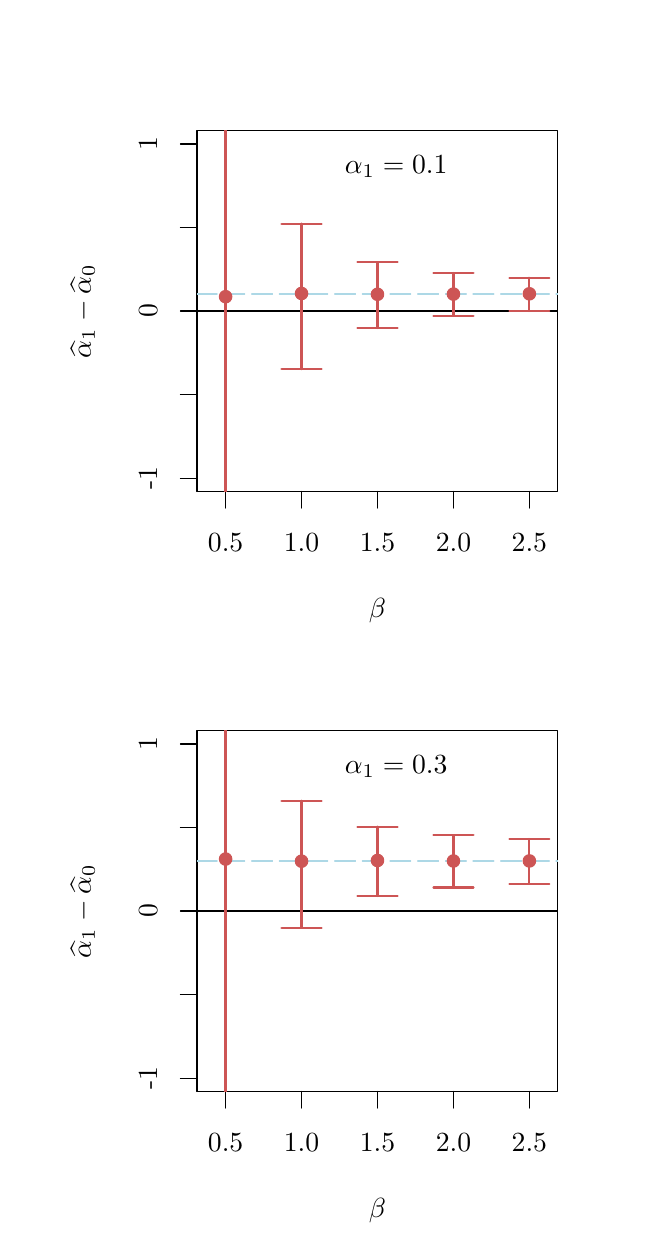
\begin{tikzpicture}[x=1pt,y=1pt]
\definecolor{fillColor}{RGB}{255,255,255}
\path[use as bounding box,fill=fillColor,fill opacity=0.00] (0,0) rectangle (216.81,433.62);
\begin{scope}
\path[clip] (  0.00,  0.00) rectangle (216.81,433.62);
\definecolor{drawColor}{RGB}{0,0,0}

\path[draw=drawColor,line width= 0.4pt,line join=round,line cap=round] ( 71.52,266.01) -- (181.29,266.01);

\path[draw=drawColor,line width= 0.4pt,line join=round,line cap=round] ( 71.52,266.01) -- ( 71.52,260.01);

\path[draw=drawColor,line width= 0.4pt,line join=round,line cap=round] ( 98.96,266.01) -- ( 98.96,260.01);

\path[draw=drawColor,line width= 0.4pt,line join=round,line cap=round] (126.40,266.01) -- (126.40,260.01);

\path[draw=drawColor,line width= 0.4pt,line join=round,line cap=round] (153.85,266.01) -- (153.85,260.01);

\path[draw=drawColor,line width= 0.4pt,line join=round,line cap=round] (181.29,266.01) -- (181.29,260.01);

\node[text=drawColor,anchor=base,inner sep=0pt, outer sep=0pt, scale=  1.00] at ( 71.52,244.41) {0.5};

\node[text=drawColor,anchor=base,inner sep=0pt, outer sep=0pt, scale=  1.00] at ( 98.96,244.41) {1.0};

\node[text=drawColor,anchor=base,inner sep=0pt, outer sep=0pt, scale=  1.00] at (126.40,244.41) {1.5};

\node[text=drawColor,anchor=base,inner sep=0pt, outer sep=0pt, scale=  1.00] at (153.85,244.41) {2.0};

\node[text=drawColor,anchor=base,inner sep=0pt, outer sep=0pt, scale=  1.00] at (181.29,244.41) {2.5};

\path[draw=drawColor,line width= 0.4pt,line join=round,line cap=round] ( 61.20,266.01) --
	(191.61,266.01) --
	(191.61,396.42) --
	( 61.20,396.42) --
	( 61.20,266.01);
\end{scope}
\begin{scope}
\path[clip] (  0.00,216.81) rectangle (216.81,433.62);
\definecolor{drawColor}{RGB}{0,0,0}

\node[text=drawColor,anchor=base,inner sep=0pt, outer sep=0pt, scale=  1.00] at (126.41,220.41) {$\beta$};

\node[text=drawColor,rotate= 90.00,anchor=base,inner sep=0pt, outer sep=0pt, scale=  1.00] at ( 22.80,331.22) {$\widehat{\alpha}_1 - \widehat{\alpha}_0$};
\end{scope}
\begin{scope}
\path[clip] (  0.00,  0.00) rectangle (216.81,433.62);
\definecolor{drawColor}{RGB}{0,0,0}

\path[draw=drawColor,line width= 0.4pt,line join=round,line cap=round] ( 61.20,270.84) -- ( 61.20,391.59);

\path[draw=drawColor,line width= 0.4pt,line join=round,line cap=round] ( 61.20,270.84) -- ( 55.20,270.84);

\path[draw=drawColor,line width= 0.4pt,line join=round,line cap=round] ( 61.20,301.03) -- ( 55.20,301.03);

\path[draw=drawColor,line width= 0.4pt,line join=round,line cap=round] ( 61.20,331.22) -- ( 55.20,331.22);

\path[draw=drawColor,line width= 0.4pt,line join=round,line cap=round] ( 61.20,361.40) -- ( 55.20,361.40);

\path[draw=drawColor,line width= 0.4pt,line join=round,line cap=round] ( 61.20,391.59) -- ( 55.20,391.59);

\node[text=drawColor,rotate= 90.00,anchor=base,inner sep=0pt, outer sep=0pt, scale=  1.00] at ( 46.80,270.84) {-1};

\node[text=drawColor,rotate= 90.00,anchor=base,inner sep=0pt, outer sep=0pt, scale=  1.00] at ( 46.80,331.22) {0};

\node[text=drawColor,rotate= 90.00,anchor=base,inner sep=0pt, outer sep=0pt, scale=  1.00] at ( 46.80,391.59) {1};
\end{scope}
\begin{scope}
\path[clip] ( 61.20,266.01) rectangle (191.61,396.42);
\definecolor{drawColor}{RGB}{0,0,0}

\node[text=drawColor,anchor=base west,inner sep=0pt, outer sep=0pt, scale=  1.00] at (114.66,380.98) {$\alpha_1=0.1$};
\definecolor{drawColor}{RGB}{173,216,230}

\path[draw=drawColor,line width= 0.8pt,dash pattern=on 7pt off 3pt ,line join=round,line cap=round] ( 61.20,337.25) -- (191.61,337.25);

\path[draw=drawColor,line width= 0.8pt,dash pattern=on 7pt off 3pt ,line join=round,line cap=round] ( 61.20,337.25) -- (191.61,337.25);

\path[draw=drawColor,line width= 0.8pt,dash pattern=on 7pt off 3pt ,line join=round,line cap=round] ( 61.20,337.25) -- (191.61,337.25);

\path[draw=drawColor,line width= 0.8pt,dash pattern=on 7pt off 3pt ,line join=round,line cap=round] ( 61.20,337.25) -- (191.61,337.25);

\path[draw=drawColor,line width= 0.8pt,dash pattern=on 7pt off 3pt ,line join=round,line cap=round] ( 61.20,337.25) -- (191.61,337.25);
\definecolor{drawColor}{RGB}{0,0,0}

\path[draw=drawColor,line width= 0.4pt,line join=round,line cap=round] ( 61.20,331.22) -- (191.61,331.22);
\definecolor{drawColor}{RGB}{205,85,85}

\path[draw=drawColor,line width= 0.8pt,line join=round,line cap=round] ( 71.52,196.78) -- ( 71.52,433.62);

\path[draw=drawColor,line width= 0.8pt,line join=round,line cap=round] ( 64.29,196.78) --
	( 71.52,196.78) --
	( 78.75,196.78);

\path[draw=drawColor,line width= 0.8pt,line join=round,line cap=round] ( 98.96,310.24) -- ( 98.96,362.80);

\path[draw=drawColor,line width= 0.8pt,line join=round,line cap=round] ( 91.73,310.24) --
	( 98.96,310.24) --
	(106.19,310.24);

\path[draw=drawColor,line width= 0.8pt,line join=round,line cap=round] (106.19,362.80) --
	( 98.96,362.80) --
	( 91.73,362.80);

\path[draw=drawColor,line width= 0.8pt,line join=round,line cap=round] (126.40,325.11) -- (126.40,348.87);

\path[draw=drawColor,line width= 0.8pt,line join=round,line cap=round] (119.18,325.11) --
	(126.40,325.11) --
	(133.63,325.11);

\path[draw=drawColor,line width= 0.8pt,line join=round,line cap=round] (133.63,348.87) --
	(126.40,348.87) --
	(119.18,348.87);

\path[draw=drawColor,line width= 0.8pt,line join=round,line cap=round] (153.85,329.48) -- (153.85,344.94);

\path[draw=drawColor,line width= 0.8pt,line join=round,line cap=round] (146.62,329.48) --
	(153.85,329.48) --
	(161.08,329.48);

\path[draw=drawColor,line width= 0.8pt,line join=round,line cap=round] (161.08,344.94) --
	(153.85,344.94) --
	(146.62,344.94);

\path[draw=drawColor,line width= 0.8pt,line join=round,line cap=round] (181.29,331.21) -- (181.29,343.28);

\path[draw=drawColor,line width= 0.8pt,line join=round,line cap=round] (174.06,331.21) --
	(181.29,331.21) --
	(188.52,331.21);

\path[draw=drawColor,line width= 0.8pt,line join=round,line cap=round] (188.52,343.28) --
	(181.29,343.28) --
	(174.06,343.28);
\definecolor{fillColor}{RGB}{205,85,85}

\path[draw=drawColor,line width= 0.4pt,line join=round,line cap=round,fill=fillColor] ( 71.52,336.41) circle (  2.25);

\path[draw=drawColor,line width= 0.4pt,line join=round,line cap=round,fill=fillColor] ( 98.96,337.57) circle (  2.25);

\path[draw=drawColor,line width= 0.4pt,line join=round,line cap=round,fill=fillColor] (126.40,337.27) circle (  2.25);

\path[draw=drawColor,line width= 0.4pt,line join=round,line cap=round,fill=fillColor] (153.85,337.34) circle (  2.25);

\path[draw=drawColor,line width= 0.4pt,line join=round,line cap=round,fill=fillColor] (181.29,337.45) circle (  2.25);
\end{scope}
\begin{scope}
\path[clip] (  0.00,  0.00) rectangle (216.81,433.62);
\definecolor{drawColor}{RGB}{0,0,0}

\path[draw=drawColor,line width= 0.4pt,line join=round,line cap=round] ( 71.52, 49.20) -- (181.29, 49.20);

\path[draw=drawColor,line width= 0.4pt,line join=round,line cap=round] ( 71.52, 49.20) -- ( 71.52, 43.20);

\path[draw=drawColor,line width= 0.4pt,line join=round,line cap=round] ( 98.96, 49.20) -- ( 98.96, 43.20);

\path[draw=drawColor,line width= 0.4pt,line join=round,line cap=round] (126.40, 49.20) -- (126.40, 43.20);

\path[draw=drawColor,line width= 0.4pt,line join=round,line cap=round] (153.85, 49.20) -- (153.85, 43.20);

\path[draw=drawColor,line width= 0.4pt,line join=round,line cap=round] (181.29, 49.20) -- (181.29, 43.20);

\node[text=drawColor,anchor=base,inner sep=0pt, outer sep=0pt, scale=  1.00] at ( 71.52, 27.60) {0.5};

\node[text=drawColor,anchor=base,inner sep=0pt, outer sep=0pt, scale=  1.00] at ( 98.96, 27.60) {1.0};

\node[text=drawColor,anchor=base,inner sep=0pt, outer sep=0pt, scale=  1.00] at (126.40, 27.60) {1.5};

\node[text=drawColor,anchor=base,inner sep=0pt, outer sep=0pt, scale=  1.00] at (153.85, 27.60) {2.0};

\node[text=drawColor,anchor=base,inner sep=0pt, outer sep=0pt, scale=  1.00] at (181.29, 27.60) {2.5};

\path[draw=drawColor,line width= 0.4pt,line join=round,line cap=round] ( 61.20, 49.20) --
	(191.61, 49.20) --
	(191.61,179.61) --
	( 61.20,179.61) --
	( 61.20, 49.20);
\end{scope}
\begin{scope}
\path[clip] (  0.00,  0.00) rectangle (216.81,216.81);
\definecolor{drawColor}{RGB}{0,0,0}

\node[text=drawColor,anchor=base,inner sep=0pt, outer sep=0pt, scale=  1.00] at (126.41,  3.60) {$\beta$};

\node[text=drawColor,rotate= 90.00,anchor=base,inner sep=0pt, outer sep=0pt, scale=  1.00] at ( 22.80,114.41) {$\widehat{\alpha}_1 - \widehat{\alpha}_0$};
\end{scope}
\begin{scope}
\path[clip] (  0.00,  0.00) rectangle (216.81,433.62);
\definecolor{drawColor}{RGB}{0,0,0}

\path[draw=drawColor,line width= 0.4pt,line join=round,line cap=round] ( 61.20, 54.03) -- ( 61.20,174.78);

\path[draw=drawColor,line width= 0.4pt,line join=round,line cap=round] ( 61.20, 54.03) -- ( 55.20, 54.03);

\path[draw=drawColor,line width= 0.4pt,line join=round,line cap=round] ( 61.20, 84.22) -- ( 55.20, 84.22);

\path[draw=drawColor,line width= 0.4pt,line join=round,line cap=round] ( 61.20,114.41) -- ( 55.20,114.41);

\path[draw=drawColor,line width= 0.4pt,line join=round,line cap=round] ( 61.20,144.59) -- ( 55.20,144.59);

\path[draw=drawColor,line width= 0.4pt,line join=round,line cap=round] ( 61.20,174.78) -- ( 55.20,174.78);

\node[text=drawColor,rotate= 90.00,anchor=base,inner sep=0pt, outer sep=0pt, scale=  1.00] at ( 46.80, 54.03) {-1};

\node[text=drawColor,rotate= 90.00,anchor=base,inner sep=0pt, outer sep=0pt, scale=  1.00] at ( 46.80,114.41) {0};

\node[text=drawColor,rotate= 90.00,anchor=base,inner sep=0pt, outer sep=0pt, scale=  1.00] at ( 46.80,174.78) {1};
\end{scope}
\begin{scope}
\path[clip] ( 61.20, 49.20) rectangle (191.61,179.61);
\definecolor{drawColor}{RGB}{0,0,0}

\node[text=drawColor,anchor=base west,inner sep=0pt, outer sep=0pt, scale=  1.00] at (114.66,164.17) {$\alpha_1=0.3$};
\definecolor{drawColor}{RGB}{173,216,230}

\path[draw=drawColor,line width= 0.8pt,dash pattern=on 7pt off 3pt ,line join=round,line cap=round] ( 61.20,132.52) -- (191.61,132.52);

\path[draw=drawColor,line width= 0.8pt,dash pattern=on 7pt off 3pt ,line join=round,line cap=round] ( 61.20,132.52) -- (191.61,132.52);

\path[draw=drawColor,line width= 0.8pt,dash pattern=on 7pt off 3pt ,line join=round,line cap=round] ( 61.20,132.52) -- (191.61,132.52);

\path[draw=drawColor,line width= 0.8pt,dash pattern=on 7pt off 3pt ,line join=round,line cap=round] ( 61.20,132.52) -- (191.61,132.52);

\path[draw=drawColor,line width= 0.8pt,dash pattern=on 7pt off 3pt ,line join=round,line cap=round] ( 61.20,132.52) -- (191.61,132.52);
\definecolor{drawColor}{RGB}{0,0,0}

\path[draw=drawColor,line width= 0.4pt,line join=round,line cap=round] ( 61.20,114.41) -- (191.61,114.41);
\definecolor{drawColor}{RGB}{205,85,85}

\path[draw=drawColor,line width= 0.8pt,line join=round,line cap=round] ( 71.52, 16.42) -- ( 71.52,249.25);

\path[draw=drawColor,line width= 0.8pt,line join=round,line cap=round] ( 64.29, 16.42) --
	( 71.52, 16.42) --
	( 78.75, 16.42);

\path[draw=drawColor,line width= 0.8pt,line join=round,line cap=round] ( 78.75,249.25) --
	( 71.52,249.25) --
	( 64.29,249.25);

\path[draw=drawColor,line width= 0.8pt,line join=round,line cap=round] ( 98.96,108.38) -- ( 98.96,154.26);

\path[draw=drawColor,line width= 0.8pt,line join=round,line cap=round] ( 91.73,108.38) --
	( 98.96,108.38) --
	(106.19,108.38);

\path[draw=drawColor,line width= 0.8pt,line join=round,line cap=round] (106.19,154.26) --
	( 98.96,154.26) --
	( 91.73,154.26);

\path[draw=drawColor,line width= 0.8pt,line join=round,line cap=round] (126.40,119.85) -- (126.40,144.90);

\path[draw=drawColor,line width= 0.8pt,line join=round,line cap=round] (119.18,119.85) --
	(126.40,119.85) --
	(133.63,119.85);

\path[draw=drawColor,line width= 0.8pt,line join=round,line cap=round] (133.63,144.90) --
	(126.40,144.90) --
	(119.18,144.90);

\path[draw=drawColor,line width= 0.8pt,line join=round,line cap=round] (153.85,122.90) -- (153.85,141.82);

\path[draw=drawColor,line width= 0.8pt,line join=round,line cap=round] (146.62,122.90) --
	(153.85,122.90) --
	(161.08,122.90);

\path[draw=drawColor,line width= 0.8pt,line join=round,line cap=round] (161.08,141.82) --
	(153.85,141.82) --
	(146.62,141.82);

\path[draw=drawColor,line width= 0.8pt,line join=round,line cap=round] (181.29,124.26) -- (181.29,140.48);

\path[draw=drawColor,line width= 0.8pt,line join=round,line cap=round] (174.06,124.26) --
	(181.29,124.26) --
	(188.52,124.26);

\path[draw=drawColor,line width= 0.8pt,line join=round,line cap=round] (188.52,140.48) --
	(181.29,140.48) --
	(174.06,140.48);
\definecolor{fillColor}{RGB}{205,85,85}

\path[draw=drawColor,line width= 0.4pt,line join=round,line cap=round,fill=fillColor] ( 71.52,133.20) circle (  2.25);

\path[draw=drawColor,line width= 0.4pt,line join=round,line cap=round,fill=fillColor] ( 98.96,132.43) circle (  2.25);

\path[draw=drawColor,line width= 0.4pt,line join=round,line cap=round,fill=fillColor] (126.40,132.68) circle (  2.25);

\path[draw=drawColor,line width= 0.4pt,line join=round,line cap=round,fill=fillColor] (153.85,132.50) circle (  2.25);

\path[draw=drawColor,line width= 0.4pt,line join=round,line cap=round,fill=fillColor] (181.29,132.52) circle (  2.25);
\end{scope}
\end{tikzpicture}

%  \end{subfigure}
%  ~
%  \begin{subfigure}[b]{0.31\textwidth}
%\caption{\footnotesize $N=5000, \delta = 0.3$}
%  % Created by tikzDevice version 0.8.1 on 2015-11-17 11:43:48
% !TEX encoding = UTF-8 Unicode
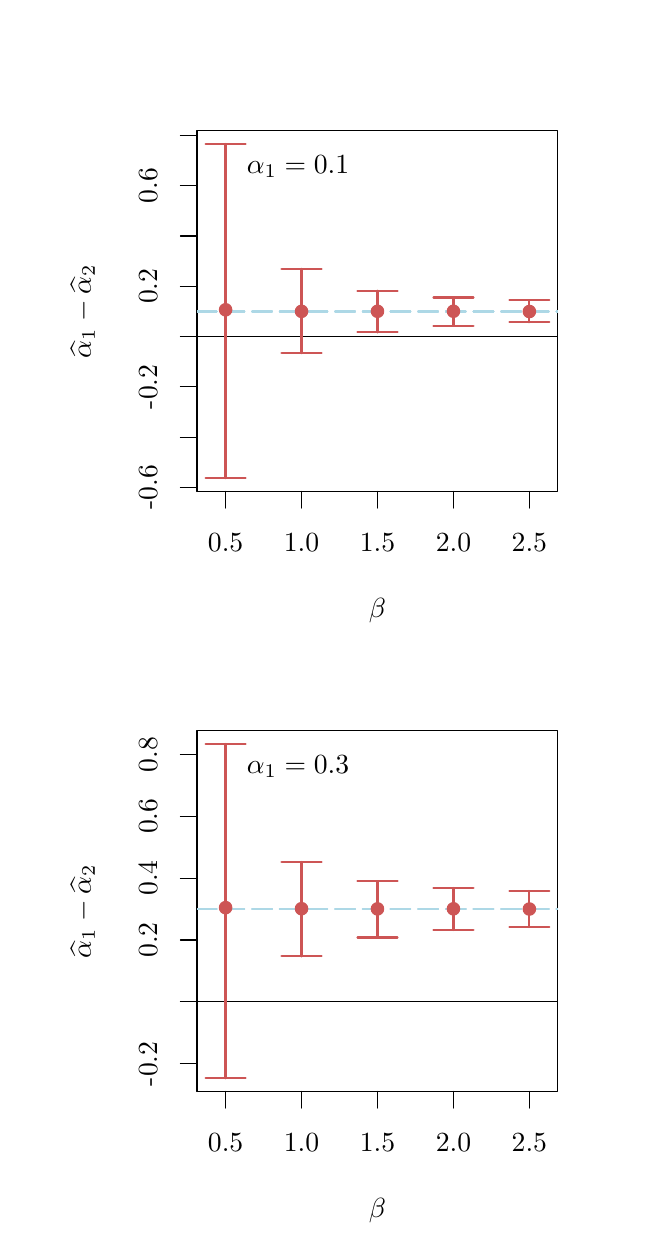
\begin{tikzpicture}[x=1pt,y=1pt]
\definecolor{fillColor}{RGB}{255,255,255}
\path[use as bounding box,fill=fillColor,fill opacity=0.00] (0,0) rectangle (216.81,433.62);
\begin{scope}
\path[clip] ( 61.20,266.01) rectangle (191.61,396.42);
\definecolor{drawColor}{RGB}{255,255,255}
\definecolor{fillColor}{RGB}{255,255,255}

\path[draw=drawColor,line width= 0.4pt,line join=round,line cap=round,fill=fillColor] ( 71.52,331.67) circle (  2.25);

\path[draw=drawColor,line width= 0.4pt,line join=round,line cap=round,fill=fillColor] ( 98.96,331.11) circle (  2.25);

\path[draw=drawColor,line width= 0.4pt,line join=round,line cap=round,fill=fillColor] (126.40,331.13) circle (  2.25);

\path[draw=drawColor,line width= 0.4pt,line join=round,line cap=round,fill=fillColor] (153.85,331.15) circle (  2.25);

\path[draw=drawColor,line width= 0.4pt,line join=round,line cap=round,fill=fillColor] (181.29,331.05) circle (  2.25);
\end{scope}
\begin{scope}
\path[clip] (  0.00,  0.00) rectangle (216.81,433.62);
\definecolor{drawColor}{RGB}{0,0,0}

\path[draw=drawColor,line width= 0.4pt,line join=round,line cap=round] ( 71.52,266.01) -- (181.29,266.01);

\path[draw=drawColor,line width= 0.4pt,line join=round,line cap=round] ( 71.52,266.01) -- ( 71.52,260.01);

\path[draw=drawColor,line width= 0.4pt,line join=round,line cap=round] ( 98.96,266.01) -- ( 98.96,260.01);

\path[draw=drawColor,line width= 0.4pt,line join=round,line cap=round] (126.40,266.01) -- (126.40,260.01);

\path[draw=drawColor,line width= 0.4pt,line join=round,line cap=round] (153.85,266.01) -- (153.85,260.01);

\path[draw=drawColor,line width= 0.4pt,line join=round,line cap=round] (181.29,266.01) -- (181.29,260.01);

\node[text=drawColor,anchor=base,inner sep=0pt, outer sep=0pt, scale=  1.00] at ( 71.52,244.41) {0.5};

\node[text=drawColor,anchor=base,inner sep=0pt, outer sep=0pt, scale=  1.00] at ( 98.96,244.41) {1.0};

\node[text=drawColor,anchor=base,inner sep=0pt, outer sep=0pt, scale=  1.00] at (126.40,244.41) {1.5};

\node[text=drawColor,anchor=base,inner sep=0pt, outer sep=0pt, scale=  1.00] at (153.85,244.41) {2.0};

\node[text=drawColor,anchor=base,inner sep=0pt, outer sep=0pt, scale=  1.00] at (181.29,244.41) {2.5};

\path[draw=drawColor,line width= 0.4pt,line join=round,line cap=round] ( 61.20,267.52) -- ( 61.20,394.65);

\path[draw=drawColor,line width= 0.4pt,line join=round,line cap=round] ( 61.20,267.52) -- ( 55.20,267.52);

\path[draw=drawColor,line width= 0.4pt,line join=round,line cap=round] ( 61.20,285.68) -- ( 55.20,285.68);

\path[draw=drawColor,line width= 0.4pt,line join=round,line cap=round] ( 61.20,303.84) -- ( 55.20,303.84);

\path[draw=drawColor,line width= 0.4pt,line join=round,line cap=round] ( 61.20,322.01) -- ( 55.20,322.01);

\path[draw=drawColor,line width= 0.4pt,line join=round,line cap=round] ( 61.20,340.17) -- ( 55.20,340.17);

\path[draw=drawColor,line width= 0.4pt,line join=round,line cap=round] ( 61.20,358.33) -- ( 55.20,358.33);

\path[draw=drawColor,line width= 0.4pt,line join=round,line cap=round] ( 61.20,376.49) -- ( 55.20,376.49);

\path[draw=drawColor,line width= 0.4pt,line join=round,line cap=round] ( 61.20,394.65) -- ( 55.20,394.65);

\node[text=drawColor,rotate= 90.00,anchor=base,inner sep=0pt, outer sep=0pt, scale=  1.00] at ( 46.80,267.52) {-0.6};

\node[text=drawColor,rotate= 90.00,anchor=base,inner sep=0pt, outer sep=0pt, scale=  1.00] at ( 46.80,303.84) {-0.2};

\node[text=drawColor,rotate= 90.00,anchor=base,inner sep=0pt, outer sep=0pt, scale=  1.00] at ( 46.80,340.17) {0.2};

\node[text=drawColor,rotate= 90.00,anchor=base,inner sep=0pt, outer sep=0pt, scale=  1.00] at ( 46.80,376.49) {0.6};

\path[draw=drawColor,line width= 0.4pt,line join=round,line cap=round] ( 61.20,266.01) --
	(191.61,266.01) --
	(191.61,396.42) --
	( 61.20,396.42) --
	( 61.20,266.01);
\end{scope}
\begin{scope}
\path[clip] (  0.00,216.81) rectangle (216.81,433.62);
\definecolor{drawColor}{RGB}{0,0,0}

\node[text=drawColor,anchor=base,inner sep=0pt, outer sep=0pt, scale=  1.00] at (126.41,220.41) {$\beta$};

\node[text=drawColor,rotate= 90.00,anchor=base,inner sep=0pt, outer sep=0pt, scale=  1.00] at ( 22.80,331.22) {$\widehat{\alpha}_1 - \widehat{\alpha}_2$};
\end{scope}
\begin{scope}
\path[clip] ( 61.20,266.01) rectangle (191.61,396.42);
\definecolor{drawColor}{RGB}{0,0,0}

\node[text=drawColor,anchor=base west,inner sep=0pt, outer sep=0pt, scale=  1.00] at ( 79.20,380.98) {$\alpha_1=0.1$};
\definecolor{drawColor}{RGB}{173,216,230}

\path[draw=drawColor,line width= 0.8pt,dash pattern=on 7pt off 3pt ,line join=round,line cap=round] ( 61.20,331.09) -- (191.61,331.09);

\path[draw=drawColor,line width= 0.8pt,dash pattern=on 7pt off 3pt ,line join=round,line cap=round] ( 61.20,331.09) -- (191.61,331.09);

\path[draw=drawColor,line width= 0.8pt,dash pattern=on 7pt off 3pt ,line join=round,line cap=round] ( 61.20,331.09) -- (191.61,331.09);

\path[draw=drawColor,line width= 0.8pt,dash pattern=on 7pt off 3pt ,line join=round,line cap=round] ( 61.20,331.09) -- (191.61,331.09);

\path[draw=drawColor,line width= 0.8pt,dash pattern=on 7pt off 3pt ,line join=round,line cap=round] ( 61.20,331.09) -- (191.61,331.09);
\definecolor{drawColor}{RGB}{0,0,0}

\path[draw=drawColor,line width= 0.4pt,line join=round,line cap=round] ( 61.20,322.01) -- (191.61,322.01);
\definecolor{drawColor}{RGB}{205,85,85}

\path[draw=drawColor,line width= 0.8pt,line join=round,line cap=round] ( 71.52,270.84) -- ( 71.52,391.59);

\path[draw=drawColor,line width= 0.8pt,line join=round,line cap=round] ( 64.29,270.84) --
	( 71.52,270.84) --
	( 78.75,270.84);

\path[draw=drawColor,line width= 0.8pt,line join=round,line cap=round] ( 78.75,391.59) --
	( 71.52,391.59) --
	( 64.29,391.59);

\path[draw=drawColor,line width= 0.8pt,line join=round,line cap=round] ( 98.96,316.02) -- ( 98.96,346.46);

\path[draw=drawColor,line width= 0.8pt,line join=round,line cap=round] ( 91.73,316.02) --
	( 98.96,316.02) --
	(106.19,316.02);

\path[draw=drawColor,line width= 0.8pt,line join=round,line cap=round] (106.19,346.46) --
	( 98.96,346.46) --
	( 91.73,346.46);

\path[draw=drawColor,line width= 0.8pt,line join=round,line cap=round] (126.40,323.52) -- (126.40,338.57);

\path[draw=drawColor,line width= 0.8pt,line join=round,line cap=round] (119.18,323.52) --
	(126.40,323.52) --
	(133.63,323.52);

\path[draw=drawColor,line width= 0.8pt,line join=round,line cap=round] (133.63,338.57) --
	(126.40,338.57) --
	(119.18,338.57);

\path[draw=drawColor,line width= 0.8pt,line join=round,line cap=round] (153.85,325.95) -- (153.85,336.11);

\path[draw=drawColor,line width= 0.8pt,line join=round,line cap=round] (146.62,325.95) --
	(153.85,325.95) --
	(161.08,325.95);

\path[draw=drawColor,line width= 0.8pt,line join=round,line cap=round] (161.08,336.11) --
	(153.85,336.11) --
	(146.62,336.11);

\path[draw=drawColor,line width= 0.8pt,line join=round,line cap=round] (181.29,327.12) -- (181.29,335.10);

\path[draw=drawColor,line width= 0.8pt,line join=round,line cap=round] (174.06,327.12) --
	(181.29,327.12) --
	(188.52,327.12);

\path[draw=drawColor,line width= 0.8pt,line join=round,line cap=round] (188.52,335.10) --
	(181.29,335.10) --
	(174.06,335.10);
\definecolor{fillColor}{RGB}{205,85,85}

\path[draw=drawColor,line width= 0.4pt,line join=round,line cap=round,fill=fillColor] ( 71.52,331.67) circle (  2.25);

\path[draw=drawColor,line width= 0.4pt,line join=round,line cap=round,fill=fillColor] ( 98.96,331.11) circle (  2.25);

\path[draw=drawColor,line width= 0.4pt,line join=round,line cap=round,fill=fillColor] (126.40,331.13) circle (  2.25);

\path[draw=drawColor,line width= 0.4pt,line join=round,line cap=round,fill=fillColor] (153.85,331.15) circle (  2.25);

\path[draw=drawColor,line width= 0.4pt,line join=round,line cap=round,fill=fillColor] (181.29,331.05) circle (  2.25);
\end{scope}
\begin{scope}
\path[clip] ( 61.20, 49.20) rectangle (191.61,179.61);
\definecolor{drawColor}{RGB}{255,255,255}
\definecolor{fillColor}{RGB}{255,255,255}

\path[draw=drawColor,line width= 0.4pt,line join=round,line cap=round,fill=fillColor] ( 71.52,115.64) circle (  2.25);

\path[draw=drawColor,line width= 0.4pt,line join=round,line cap=round,fill=fillColor] ( 98.96,115.26) circle (  2.25);

\path[draw=drawColor,line width= 0.4pt,line join=round,line cap=round,fill=fillColor] (126.40,115.19) circle (  2.25);

\path[draw=drawColor,line width= 0.4pt,line join=round,line cap=round,fill=fillColor] (153.85,115.22) circle (  2.25);

\path[draw=drawColor,line width= 0.4pt,line join=round,line cap=round,fill=fillColor] (181.29,115.14) circle (  2.25);
\end{scope}
\begin{scope}
\path[clip] (  0.00,  0.00) rectangle (216.81,433.62);
\definecolor{drawColor}{RGB}{0,0,0}

\path[draw=drawColor,line width= 0.4pt,line join=round,line cap=round] ( 71.52, 49.20) -- (181.29, 49.20);

\path[draw=drawColor,line width= 0.4pt,line join=round,line cap=round] ( 71.52, 49.20) -- ( 71.52, 43.20);

\path[draw=drawColor,line width= 0.4pt,line join=round,line cap=round] ( 98.96, 49.20) -- ( 98.96, 43.20);

\path[draw=drawColor,line width= 0.4pt,line join=round,line cap=round] (126.40, 49.20) -- (126.40, 43.20);

\path[draw=drawColor,line width= 0.4pt,line join=round,line cap=round] (153.85, 49.20) -- (153.85, 43.20);

\path[draw=drawColor,line width= 0.4pt,line join=round,line cap=round] (181.29, 49.20) -- (181.29, 43.20);

\node[text=drawColor,anchor=base,inner sep=0pt, outer sep=0pt, scale=  1.00] at ( 71.52, 27.60) {0.5};

\node[text=drawColor,anchor=base,inner sep=0pt, outer sep=0pt, scale=  1.00] at ( 98.96, 27.60) {1.0};

\node[text=drawColor,anchor=base,inner sep=0pt, outer sep=0pt, scale=  1.00] at (126.40, 27.60) {1.5};

\node[text=drawColor,anchor=base,inner sep=0pt, outer sep=0pt, scale=  1.00] at (153.85, 27.60) {2.0};

\node[text=drawColor,anchor=base,inner sep=0pt, outer sep=0pt, scale=  1.00] at (181.29, 27.60) {2.5};

\path[draw=drawColor,line width= 0.4pt,line join=round,line cap=round] ( 61.20, 59.22) -- ( 61.20,171.04);

\path[draw=drawColor,line width= 0.4pt,line join=round,line cap=round] ( 61.20, 59.22) -- ( 55.20, 59.22);

\path[draw=drawColor,line width= 0.4pt,line join=round,line cap=round] ( 61.20, 81.58) -- ( 55.20, 81.58);

\path[draw=drawColor,line width= 0.4pt,line join=round,line cap=round] ( 61.20,103.95) -- ( 55.20,103.95);

\path[draw=drawColor,line width= 0.4pt,line join=round,line cap=round] ( 61.20,126.31) -- ( 55.20,126.31);

\path[draw=drawColor,line width= 0.4pt,line join=round,line cap=round] ( 61.20,148.68) -- ( 55.20,148.68);

\path[draw=drawColor,line width= 0.4pt,line join=round,line cap=round] ( 61.20,171.04) -- ( 55.20,171.04);

\node[text=drawColor,rotate= 90.00,anchor=base,inner sep=0pt, outer sep=0pt, scale=  1.00] at ( 46.80, 59.22) {-0.2};

\node[text=drawColor,rotate= 90.00,anchor=base,inner sep=0pt, outer sep=0pt, scale=  1.00] at ( 46.80,103.95) {0.2};

\node[text=drawColor,rotate= 90.00,anchor=base,inner sep=0pt, outer sep=0pt, scale=  1.00] at ( 46.80,126.31) {0.4};

\node[text=drawColor,rotate= 90.00,anchor=base,inner sep=0pt, outer sep=0pt, scale=  1.00] at ( 46.80,148.68) {0.6};

\node[text=drawColor,rotate= 90.00,anchor=base,inner sep=0pt, outer sep=0pt, scale=  1.00] at ( 46.80,171.04) {0.8};

\path[draw=drawColor,line width= 0.4pt,line join=round,line cap=round] ( 61.20, 49.20) --
	(191.61, 49.20) --
	(191.61,179.61) --
	( 61.20,179.61) --
	( 61.20, 49.20);
\end{scope}
\begin{scope}
\path[clip] (  0.00,  0.00) rectangle (216.81,216.81);
\definecolor{drawColor}{RGB}{0,0,0}

\node[text=drawColor,anchor=base,inner sep=0pt, outer sep=0pt, scale=  1.00] at (126.41,  3.60) {$\beta$};

\node[text=drawColor,rotate= 90.00,anchor=base,inner sep=0pt, outer sep=0pt, scale=  1.00] at ( 22.80,114.41) {$\widehat{\alpha}_1 - \widehat{\alpha}_2$};
\end{scope}
\begin{scope}
\path[clip] ( 61.20, 49.20) rectangle (191.61,179.61);
\definecolor{drawColor}{RGB}{0,0,0}

\node[text=drawColor,anchor=base west,inner sep=0pt, outer sep=0pt, scale=  1.00] at ( 79.20,164.17) {$\alpha_1=0.3$};
\definecolor{drawColor}{RGB}{173,216,230}

\path[draw=drawColor,line width= 0.8pt,dash pattern=on 7pt off 3pt ,line join=round,line cap=round] ( 61.20,115.13) -- (191.61,115.13);

\path[draw=drawColor,line width= 0.8pt,dash pattern=on 7pt off 3pt ,line join=round,line cap=round] ( 61.20,115.13) -- (191.61,115.13);

\path[draw=drawColor,line width= 0.8pt,dash pattern=on 7pt off 3pt ,line join=round,line cap=round] ( 61.20,115.13) -- (191.61,115.13);

\path[draw=drawColor,line width= 0.8pt,dash pattern=on 7pt off 3pt ,line join=round,line cap=round] ( 61.20,115.13) -- (191.61,115.13);

\path[draw=drawColor,line width= 0.8pt,dash pattern=on 7pt off 3pt ,line join=round,line cap=round] ( 61.20,115.13) -- (191.61,115.13);
\definecolor{drawColor}{RGB}{0,0,0}

\path[draw=drawColor,line width= 0.4pt,line join=round,line cap=round] ( 61.20, 81.58) -- (191.61, 81.58);
\definecolor{drawColor}{RGB}{205,85,85}

\path[draw=drawColor,line width= 0.8pt,line join=round,line cap=round] ( 71.52, 54.03) -- ( 71.52,174.78);

\path[draw=drawColor,line width= 0.8pt,line join=round,line cap=round] ( 64.29, 54.03) --
	( 71.52, 54.03) --
	( 78.75, 54.03);

\path[draw=drawColor,line width= 0.8pt,line join=round,line cap=round] ( 78.75,174.78) --
	( 71.52,174.78) --
	( 64.29,174.78);

\path[draw=drawColor,line width= 0.8pt,line join=round,line cap=round] ( 98.96, 98.04) -- ( 98.96,132.11);

\path[draw=drawColor,line width= 0.8pt,line join=round,line cap=round] ( 91.73, 98.04) --
	( 98.96, 98.04) --
	(106.19, 98.04);

\path[draw=drawColor,line width= 0.8pt,line join=round,line cap=round] (106.19,132.11) --
	( 98.96,132.11) --
	( 91.73,132.11);

\path[draw=drawColor,line width= 0.8pt,line join=round,line cap=round] (126.40,104.88) -- (126.40,125.22);

\path[draw=drawColor,line width= 0.8pt,line join=round,line cap=round] (119.18,104.88) --
	(126.40,104.88) --
	(133.63,104.88);

\path[draw=drawColor,line width= 0.8pt,line join=round,line cap=round] (133.63,125.22) --
	(126.40,125.22) --
	(119.18,125.22);

\path[draw=drawColor,line width= 0.8pt,line join=round,line cap=round] (153.85,107.55) -- (153.85,122.74);

\path[draw=drawColor,line width= 0.8pt,line join=round,line cap=round] (146.62,107.55) --
	(153.85,107.55) --
	(161.08,107.55);

\path[draw=drawColor,line width= 0.8pt,line join=round,line cap=round] (161.08,122.74) --
	(153.85,122.74) --
	(146.62,122.74);

\path[draw=drawColor,line width= 0.8pt,line join=round,line cap=round] (181.29,108.66) -- (181.29,121.64);

\path[draw=drawColor,line width= 0.8pt,line join=round,line cap=round] (174.06,108.66) --
	(181.29,108.66) --
	(188.52,108.66);

\path[draw=drawColor,line width= 0.8pt,line join=round,line cap=round] (188.52,121.64) --
	(181.29,121.64) --
	(174.06,121.64);
\definecolor{fillColor}{RGB}{205,85,85}

\path[draw=drawColor,line width= 0.4pt,line join=round,line cap=round,fill=fillColor] ( 71.52,115.64) circle (  2.25);

\path[draw=drawColor,line width= 0.4pt,line join=round,line cap=round,fill=fillColor] ( 98.96,115.26) circle (  2.25);

\path[draw=drawColor,line width= 0.4pt,line join=round,line cap=round,fill=fillColor] (126.40,115.19) circle (  2.25);

\path[draw=drawColor,line width= 0.4pt,line join=round,line cap=round,fill=fillColor] (153.85,115.22) circle (  2.25);

\path[draw=drawColor,line width= 0.4pt,line join=round,line cap=round,fill=fillColor] (181.29,115.14) circle (  2.25);
\end{scope}
\end{tikzpicture}

%  \end{subfigure}
%\endgroup
%\end{figure}
%\end{frame}
%%%%%%%%%%%%%%%%%%%%%%%%%%%%%%%%%%%%%%%
%\begin{frame}
%  \begin{center}
%    {\framebox{\Large Sampling Distribution of $\widehat{\beta} = (1 - \widehat{\alpha}_0 - \widehat{\alpha}_1)\widehat{\beta}_{IV}$}}
%  \end{center}
%\end{frame}
%%%%%%%%%%%%%%%%%%%%%%%%%%%%%%%%%%%%%%%
%\begin{frame}
%\begin{figure}[h]
%  \scriptsize
%  \begingroup
%  \tikzset{every picture/.style={scale=0.53}}
%  \centering
%  \begin{subfigure}[b]{0.31\textwidth}
%\caption{\footnotesize $N=500, \delta = 0.1$}
%  % Created by tikzDevice version 0.8.1 on 2015-11-17 12:57:40
% !TEX encoding = UTF-8 Unicode
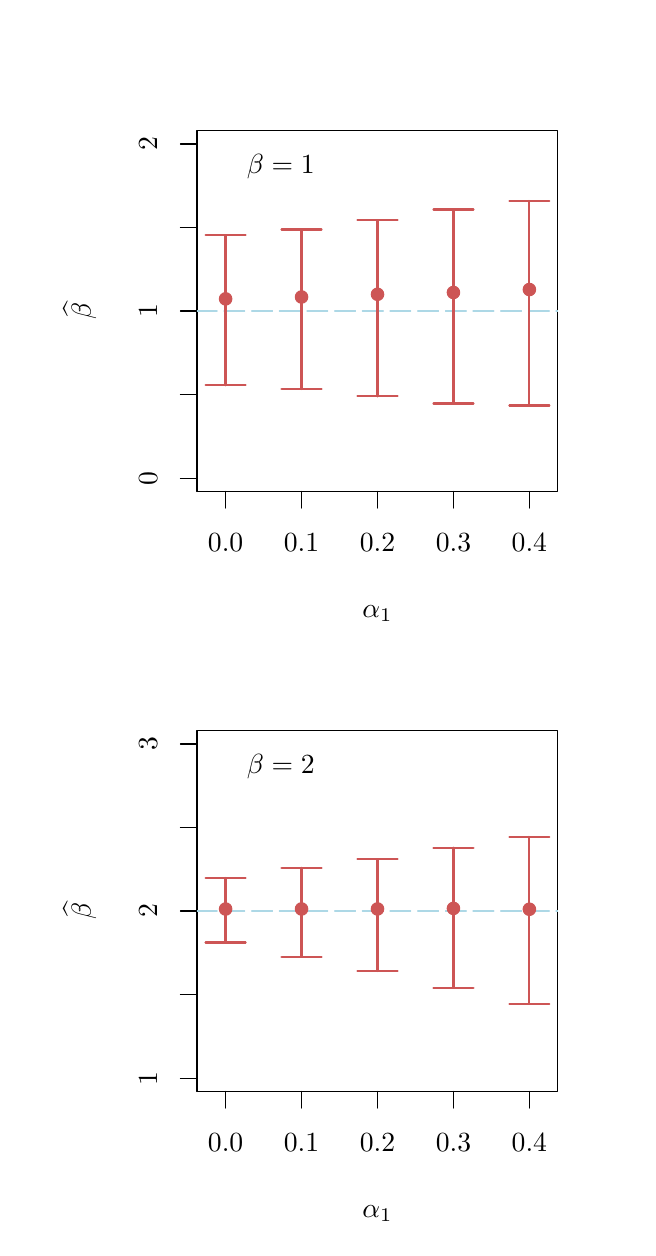
\begin{tikzpicture}[x=1pt,y=1pt]
\definecolor{fillColor}{RGB}{255,255,255}
\path[use as bounding box,fill=fillColor,fill opacity=0.00] (0,0) rectangle (216.81,433.62);
\begin{scope}
\path[clip] (  0.00,  0.00) rectangle (216.81,433.62);
\definecolor{drawColor}{RGB}{0,0,0}

\path[draw=drawColor,line width= 0.4pt,line join=round,line cap=round] ( 71.52,266.01) -- (181.29,266.01);

\path[draw=drawColor,line width= 0.4pt,line join=round,line cap=round] ( 71.52,266.01) -- ( 71.52,260.01);

\path[draw=drawColor,line width= 0.4pt,line join=round,line cap=round] ( 98.96,266.01) -- ( 98.96,260.01);

\path[draw=drawColor,line width= 0.4pt,line join=round,line cap=round] (126.41,266.01) -- (126.41,260.01);

\path[draw=drawColor,line width= 0.4pt,line join=round,line cap=round] (153.85,266.01) -- (153.85,260.01);

\path[draw=drawColor,line width= 0.4pt,line join=round,line cap=round] (181.29,266.01) -- (181.29,260.01);

\node[text=drawColor,anchor=base,inner sep=0pt, outer sep=0pt, scale=  1.00] at ( 71.52,244.41) {0.0};

\node[text=drawColor,anchor=base,inner sep=0pt, outer sep=0pt, scale=  1.00] at ( 98.96,244.41) {0.1};

\node[text=drawColor,anchor=base,inner sep=0pt, outer sep=0pt, scale=  1.00] at (126.41,244.41) {0.2};

\node[text=drawColor,anchor=base,inner sep=0pt, outer sep=0pt, scale=  1.00] at (153.85,244.41) {0.3};

\node[text=drawColor,anchor=base,inner sep=0pt, outer sep=0pt, scale=  1.00] at (181.29,244.41) {0.4};

\path[draw=drawColor,line width= 0.4pt,line join=round,line cap=round] ( 61.20,266.01) --
	(191.61,266.01) --
	(191.61,396.42) --
	( 61.20,396.42) --
	( 61.20,266.01);
\end{scope}
\begin{scope}
\path[clip] (  0.00,216.81) rectangle (216.81,433.62);
\definecolor{drawColor}{RGB}{0,0,0}

\node[text=drawColor,anchor=base,inner sep=0pt, outer sep=0pt, scale=  1.00] at (126.41,220.41) {$\alpha_1$};

\node[text=drawColor,rotate= 90.00,anchor=base,inner sep=0pt, outer sep=0pt, scale=  1.00] at ( 22.80,331.22) {$\widehat{\beta}$};
\end{scope}
\begin{scope}
\path[clip] (  0.00,  0.00) rectangle (216.81,433.62);
\definecolor{drawColor}{RGB}{0,0,0}

\path[draw=drawColor,line width= 0.4pt,line join=round,line cap=round] ( 61.20,270.84) -- ( 61.20,391.59);

\path[draw=drawColor,line width= 0.4pt,line join=round,line cap=round] ( 61.20,270.84) -- ( 55.20,270.84);

\path[draw=drawColor,line width= 0.4pt,line join=round,line cap=round] ( 61.20,301.03) -- ( 55.20,301.03);

\path[draw=drawColor,line width= 0.4pt,line join=round,line cap=round] ( 61.20,331.22) -- ( 55.20,331.22);

\path[draw=drawColor,line width= 0.4pt,line join=round,line cap=round] ( 61.20,361.40) -- ( 55.20,361.40);

\path[draw=drawColor,line width= 0.4pt,line join=round,line cap=round] ( 61.20,391.59) -- ( 55.20,391.59);

\node[text=drawColor,rotate= 90.00,anchor=base,inner sep=0pt, outer sep=0pt, scale=  1.00] at ( 46.80,270.84) {0};

\node[text=drawColor,rotate= 90.00,anchor=base,inner sep=0pt, outer sep=0pt, scale=  1.00] at ( 46.80,331.22) {1};

\node[text=drawColor,rotate= 90.00,anchor=base,inner sep=0pt, outer sep=0pt, scale=  1.00] at ( 46.80,391.59) {2};
\end{scope}
\begin{scope}
\path[clip] ( 61.20,266.01) rectangle (191.61,396.42);
\definecolor{drawColor}{RGB}{0,0,0}

\node[text=drawColor,anchor=base west,inner sep=0pt, outer sep=0pt, scale=  1.00] at ( 79.20,380.98) {$\beta=1$};
\definecolor{drawColor}{RGB}{173,216,230}

\path[draw=drawColor,line width= 0.8pt,dash pattern=on 7pt off 3pt ,line join=round,line cap=round] ( 61.20,331.22) -- (191.61,331.22);

\path[draw=drawColor,line width= 0.8pt,dash pattern=on 7pt off 3pt ,line join=round,line cap=round] ( 61.20,331.22) -- (191.61,331.22);

\path[draw=drawColor,line width= 0.8pt,dash pattern=on 7pt off 3pt ,line join=round,line cap=round] ( 61.20,331.22) -- (191.61,331.22);

\path[draw=drawColor,line width= 0.8pt,dash pattern=on 7pt off 3pt ,line join=round,line cap=round] ( 61.20,331.22) -- (191.61,331.22);

\path[draw=drawColor,line width= 0.8pt,dash pattern=on 7pt off 3pt ,line join=round,line cap=round] ( 61.20,331.22) -- (191.61,331.22);
\definecolor{drawColor}{RGB}{205,85,85}

\path[draw=drawColor,line width= 0.8pt,line join=round,line cap=round] ( 71.52,304.43) -- ( 71.52,358.60);

\path[draw=drawColor,line width= 0.8pt,line join=round,line cap=round] ( 64.29,304.43) --
	( 71.52,304.43) --
	( 78.75,304.43);

\path[draw=drawColor,line width= 0.8pt,line join=round,line cap=round] ( 78.75,358.60) --
	( 71.52,358.60) --
	( 64.29,358.60);

\path[draw=drawColor,line width= 0.8pt,line join=round,line cap=round] ( 98.96,303.04) -- ( 98.96,360.66);

\path[draw=drawColor,line width= 0.8pt,line join=round,line cap=round] ( 91.73,303.04) --
	( 98.96,303.04) --
	(106.19,303.04);

\path[draw=drawColor,line width= 0.8pt,line join=round,line cap=round] (106.19,360.66) --
	( 98.96,360.66) --
	( 91.73,360.66);

\path[draw=drawColor,line width= 0.8pt,line join=round,line cap=round] (126.41,300.38) -- (126.41,364.05);

\path[draw=drawColor,line width= 0.8pt,line join=round,line cap=round] (119.18,300.38) --
	(126.41,300.38) --
	(133.63,300.38);

\path[draw=drawColor,line width= 0.8pt,line join=round,line cap=round] (133.63,364.05) --
	(126.41,364.05) --
	(119.18,364.05);

\path[draw=drawColor,line width= 0.8pt,line join=round,line cap=round] (153.85,297.78) -- (153.85,367.94);

\path[draw=drawColor,line width= 0.8pt,line join=round,line cap=round] (146.62,297.78) --
	(153.85,297.78) --
	(161.08,297.78);

\path[draw=drawColor,line width= 0.8pt,line join=round,line cap=round] (161.08,367.94) --
	(153.85,367.94) --
	(146.62,367.94);

\path[draw=drawColor,line width= 0.8pt,line join=round,line cap=round] (181.29,297.06) -- (181.29,371.01);

\path[draw=drawColor,line width= 0.8pt,line join=round,line cap=round] (174.06,297.06) --
	(181.29,297.06) --
	(188.52,297.06);

\path[draw=drawColor,line width= 0.8pt,line join=round,line cap=round] (188.52,371.01) --
	(181.29,371.01) --
	(174.06,371.01);
\definecolor{fillColor}{RGB}{205,85,85}

\path[draw=drawColor,line width= 0.4pt,line join=round,line cap=round,fill=fillColor] ( 71.52,335.62) circle (  2.25);

\path[draw=drawColor,line width= 0.4pt,line join=round,line cap=round,fill=fillColor] ( 98.96,336.30) circle (  2.25);

\path[draw=drawColor,line width= 0.4pt,line join=round,line cap=round,fill=fillColor] (126.41,337.27) circle (  2.25);

\path[draw=drawColor,line width= 0.4pt,line join=round,line cap=round,fill=fillColor] (153.85,337.93) circle (  2.25);

\path[draw=drawColor,line width= 0.4pt,line join=round,line cap=round,fill=fillColor] (181.29,338.99) circle (  2.25);
\end{scope}
\begin{scope}
\path[clip] (  0.00,  0.00) rectangle (216.81,433.62);
\definecolor{drawColor}{RGB}{0,0,0}

\path[draw=drawColor,line width= 0.4pt,line join=round,line cap=round] ( 71.52, 49.20) -- (181.29, 49.20);

\path[draw=drawColor,line width= 0.4pt,line join=round,line cap=round] ( 71.52, 49.20) -- ( 71.52, 43.20);

\path[draw=drawColor,line width= 0.4pt,line join=round,line cap=round] ( 98.96, 49.20) -- ( 98.96, 43.20);

\path[draw=drawColor,line width= 0.4pt,line join=round,line cap=round] (126.41, 49.20) -- (126.41, 43.20);

\path[draw=drawColor,line width= 0.4pt,line join=round,line cap=round] (153.85, 49.20) -- (153.85, 43.20);

\path[draw=drawColor,line width= 0.4pt,line join=round,line cap=round] (181.29, 49.20) -- (181.29, 43.20);

\node[text=drawColor,anchor=base,inner sep=0pt, outer sep=0pt, scale=  1.00] at ( 71.52, 27.60) {0.0};

\node[text=drawColor,anchor=base,inner sep=0pt, outer sep=0pt, scale=  1.00] at ( 98.96, 27.60) {0.1};

\node[text=drawColor,anchor=base,inner sep=0pt, outer sep=0pt, scale=  1.00] at (126.41, 27.60) {0.2};

\node[text=drawColor,anchor=base,inner sep=0pt, outer sep=0pt, scale=  1.00] at (153.85, 27.60) {0.3};

\node[text=drawColor,anchor=base,inner sep=0pt, outer sep=0pt, scale=  1.00] at (181.29, 27.60) {0.4};

\path[draw=drawColor,line width= 0.4pt,line join=round,line cap=round] ( 61.20, 49.20) --
	(191.61, 49.20) --
	(191.61,179.61) --
	( 61.20,179.61) --
	( 61.20, 49.20);
\end{scope}
\begin{scope}
\path[clip] (  0.00,  0.00) rectangle (216.81,216.81);
\definecolor{drawColor}{RGB}{0,0,0}

\node[text=drawColor,anchor=base,inner sep=0pt, outer sep=0pt, scale=  1.00] at (126.41,  3.60) {$\alpha_1$};

\node[text=drawColor,rotate= 90.00,anchor=base,inner sep=0pt, outer sep=0pt, scale=  1.00] at ( 22.80,114.41) {$\widehat{\beta}$};
\end{scope}
\begin{scope}
\path[clip] (  0.00,  0.00) rectangle (216.81,433.62);
\definecolor{drawColor}{RGB}{0,0,0}

\path[draw=drawColor,line width= 0.4pt,line join=round,line cap=round] ( 61.20, 54.03) -- ( 61.20,174.78);

\path[draw=drawColor,line width= 0.4pt,line join=round,line cap=round] ( 61.20, 54.03) -- ( 55.20, 54.03);

\path[draw=drawColor,line width= 0.4pt,line join=round,line cap=round] ( 61.20, 84.22) -- ( 55.20, 84.22);

\path[draw=drawColor,line width= 0.4pt,line join=round,line cap=round] ( 61.20,114.41) -- ( 55.20,114.41);

\path[draw=drawColor,line width= 0.4pt,line join=round,line cap=round] ( 61.20,144.59) -- ( 55.20,144.59);

\path[draw=drawColor,line width= 0.4pt,line join=round,line cap=round] ( 61.20,174.78) -- ( 55.20,174.78);

\node[text=drawColor,rotate= 90.00,anchor=base,inner sep=0pt, outer sep=0pt, scale=  1.00] at ( 46.80, 54.03) {1};

\node[text=drawColor,rotate= 90.00,anchor=base,inner sep=0pt, outer sep=0pt, scale=  1.00] at ( 46.80,114.41) {2};

\node[text=drawColor,rotate= 90.00,anchor=base,inner sep=0pt, outer sep=0pt, scale=  1.00] at ( 46.80,174.78) {3};
\end{scope}
\begin{scope}
\path[clip] ( 61.20, 49.20) rectangle (191.61,179.61);
\definecolor{drawColor}{RGB}{0,0,0}

\node[text=drawColor,anchor=base west,inner sep=0pt, outer sep=0pt, scale=  1.00] at ( 79.20,164.17) {$\beta=2$};
\definecolor{drawColor}{RGB}{173,216,230}

\path[draw=drawColor,line width= 0.8pt,dash pattern=on 7pt off 3pt ,line join=round,line cap=round] ( 61.20,114.41) -- (191.61,114.41);

\path[draw=drawColor,line width= 0.8pt,dash pattern=on 7pt off 3pt ,line join=round,line cap=round] ( 61.20,114.41) -- (191.61,114.41);

\path[draw=drawColor,line width= 0.8pt,dash pattern=on 7pt off 3pt ,line join=round,line cap=round] ( 61.20,114.41) -- (191.61,114.41);

\path[draw=drawColor,line width= 0.8pt,dash pattern=on 7pt off 3pt ,line join=round,line cap=round] ( 61.20,114.41) -- (191.61,114.41);

\path[draw=drawColor,line width= 0.8pt,dash pattern=on 7pt off 3pt ,line join=round,line cap=round] ( 61.20,114.41) -- (191.61,114.41);
\definecolor{drawColor}{RGB}{205,85,85}

\path[draw=drawColor,line width= 0.8pt,line join=round,line cap=round] ( 71.52,103.04) -- ( 71.52,126.36);

\path[draw=drawColor,line width= 0.8pt,line join=round,line cap=round] ( 64.29,103.04) --
	( 71.52,103.04) --
	( 78.75,103.04);

\path[draw=drawColor,line width= 0.8pt,line join=round,line cap=round] ( 78.75,126.36) --
	( 71.52,126.36) --
	( 64.29,126.36);

\path[draw=drawColor,line width= 0.8pt,line join=round,line cap=round] ( 98.96, 97.91) -- ( 98.96,130.00);

\path[draw=drawColor,line width= 0.8pt,line join=round,line cap=round] ( 91.73, 97.91) --
	( 98.96, 97.91) --
	(106.19, 97.91);

\path[draw=drawColor,line width= 0.8pt,line join=round,line cap=round] (106.19,130.00) --
	( 98.96,130.00) --
	( 91.73,130.00);

\path[draw=drawColor,line width= 0.8pt,line join=round,line cap=round] (126.41, 92.74) -- (126.41,133.08);

\path[draw=drawColor,line width= 0.8pt,line join=round,line cap=round] (119.18, 92.74) --
	(126.41, 92.74) --
	(133.63, 92.74);

\path[draw=drawColor,line width= 0.8pt,line join=round,line cap=round] (133.63,133.08) --
	(126.41,133.08) --
	(119.18,133.08);

\path[draw=drawColor,line width= 0.8pt,line join=round,line cap=round] (153.85, 86.73) -- (153.85,137.30);

\path[draw=drawColor,line width= 0.8pt,line join=round,line cap=round] (146.62, 86.73) --
	(153.85, 86.73) --
	(161.08, 86.73);

\path[draw=drawColor,line width= 0.8pt,line join=round,line cap=round] (161.08,137.30) --
	(153.85,137.30) --
	(146.62,137.30);

\path[draw=drawColor,line width= 0.8pt,line join=round,line cap=round] (181.29, 80.88) -- (181.29,141.22);

\path[draw=drawColor,line width= 0.8pt,line join=round,line cap=round] (174.06, 80.88) --
	(181.29, 80.88) --
	(188.52, 80.88);

\path[draw=drawColor,line width= 0.8pt,line join=round,line cap=round] (188.52,141.22) --
	(181.29,141.22) --
	(174.06,141.22);
\definecolor{fillColor}{RGB}{205,85,85}

\path[draw=drawColor,line width= 0.4pt,line join=round,line cap=round,fill=fillColor] ( 71.52,115.14) circle (  2.25);

\path[draw=drawColor,line width= 0.4pt,line join=round,line cap=round,fill=fillColor] ( 98.96,115.16) circle (  2.25);

\path[draw=drawColor,line width= 0.4pt,line join=round,line cap=round,fill=fillColor] (126.41,115.17) circle (  2.25);

\path[draw=drawColor,line width= 0.4pt,line join=round,line cap=round,fill=fillColor] (153.85,115.37) circle (  2.25);

\path[draw=drawColor,line width= 0.4pt,line join=round,line cap=round,fill=fillColor] (181.29,115.06) circle (  2.25);
\end{scope}
\end{tikzpicture}

%  \end{subfigure}
%  ~
%  \begin{subfigure}[b]{0.31\textwidth}
%    \caption{\footnotesize $N=1000, \delta = 0.1$} 
%  % Created by tikzDevice version 0.8.1 on 2015-11-17 12:15:23
% !TEX encoding = UTF-8 Unicode
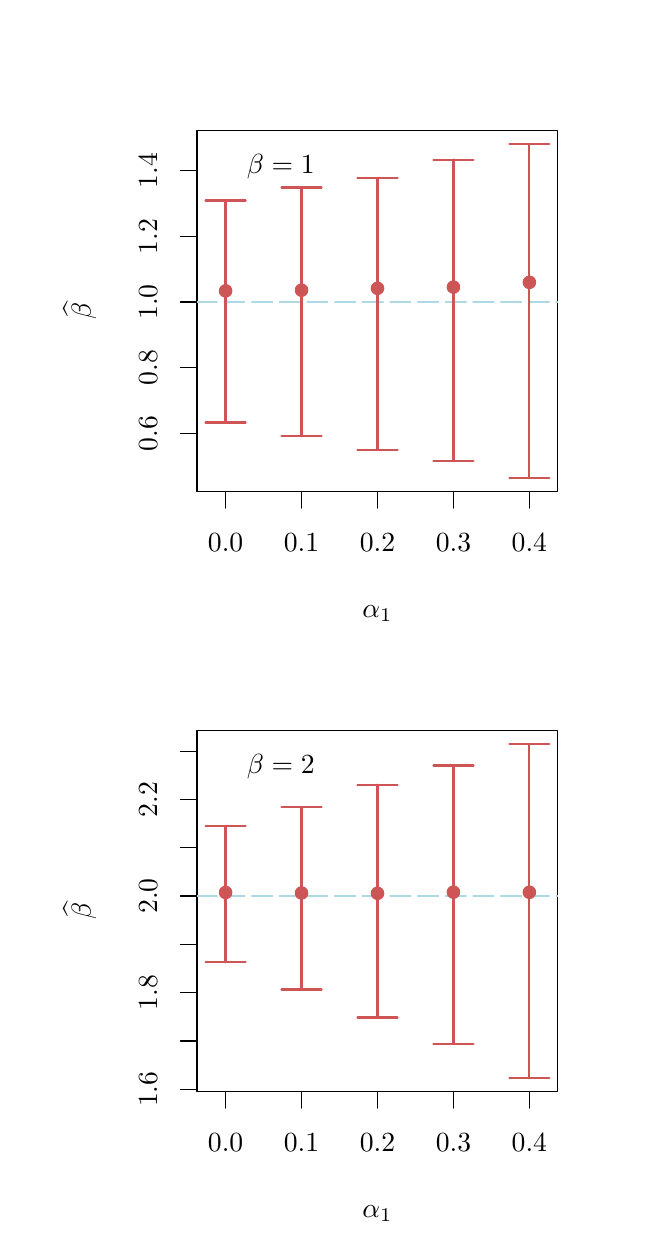
\begin{tikzpicture}[x=1pt,y=1pt]
\definecolor{fillColor}{RGB}{255,255,255}
\path[use as bounding box,fill=fillColor,fill opacity=0.00] (0,0) rectangle (216.81,433.62);
\begin{scope}
\path[clip] ( 61.20,266.01) rectangle (191.61,396.42);
\definecolor{drawColor}{RGB}{255,255,255}
\definecolor{fillColor}{RGB}{255,255,255}

\path[draw=drawColor,line width= 0.4pt,line join=round,line cap=round,fill=fillColor] ( 71.52,338.50) circle (  2.25);

\path[draw=drawColor,line width= 0.4pt,line join=round,line cap=round,fill=fillColor] ( 98.96,338.76) circle (  2.25);

\path[draw=drawColor,line width= 0.4pt,line join=round,line cap=round,fill=fillColor] (126.41,339.43) circle (  2.25);

\path[draw=drawColor,line width= 0.4pt,line join=round,line cap=round,fill=fillColor] (153.85,339.87) circle (  2.25);

\path[draw=drawColor,line width= 0.4pt,line join=round,line cap=round,fill=fillColor] (181.29,341.59) circle (  2.25);
\end{scope}
\begin{scope}
\path[clip] (  0.00,  0.00) rectangle (216.81,433.62);
\definecolor{drawColor}{RGB}{0,0,0}

\path[draw=drawColor,line width= 0.4pt,line join=round,line cap=round] ( 71.52,266.01) -- (181.29,266.01);

\path[draw=drawColor,line width= 0.4pt,line join=round,line cap=round] ( 71.52,266.01) -- ( 71.52,260.01);

\path[draw=drawColor,line width= 0.4pt,line join=round,line cap=round] ( 98.96,266.01) -- ( 98.96,260.01);

\path[draw=drawColor,line width= 0.4pt,line join=round,line cap=round] (126.41,266.01) -- (126.41,260.01);

\path[draw=drawColor,line width= 0.4pt,line join=round,line cap=round] (153.85,266.01) -- (153.85,260.01);

\path[draw=drawColor,line width= 0.4pt,line join=round,line cap=round] (181.29,266.01) -- (181.29,260.01);

\node[text=drawColor,anchor=base,inner sep=0pt, outer sep=0pt, scale=  1.00] at ( 71.52,244.41) {0.0};

\node[text=drawColor,anchor=base,inner sep=0pt, outer sep=0pt, scale=  1.00] at ( 98.96,244.41) {0.1};

\node[text=drawColor,anchor=base,inner sep=0pt, outer sep=0pt, scale=  1.00] at (126.41,244.41) {0.2};

\node[text=drawColor,anchor=base,inner sep=0pt, outer sep=0pt, scale=  1.00] at (153.85,244.41) {0.3};

\node[text=drawColor,anchor=base,inner sep=0pt, outer sep=0pt, scale=  1.00] at (181.29,244.41) {0.4};

\path[draw=drawColor,line width= 0.4pt,line join=round,line cap=round] ( 61.20,287.03) -- ( 61.20,381.92);

\path[draw=drawColor,line width= 0.4pt,line join=round,line cap=round] ( 61.20,287.03) -- ( 55.20,287.03);

\path[draw=drawColor,line width= 0.4pt,line join=round,line cap=round] ( 61.20,310.75) -- ( 55.20,310.75);

\path[draw=drawColor,line width= 0.4pt,line join=round,line cap=round] ( 61.20,334.48) -- ( 55.20,334.48);

\path[draw=drawColor,line width= 0.4pt,line join=round,line cap=round] ( 61.20,358.20) -- ( 55.20,358.20);

\path[draw=drawColor,line width= 0.4pt,line join=round,line cap=round] ( 61.20,381.92) -- ( 55.20,381.92);

\node[text=drawColor,rotate= 90.00,anchor=base,inner sep=0pt, outer sep=0pt, scale=  1.00] at ( 46.80,287.03) {0.6};

\node[text=drawColor,rotate= 90.00,anchor=base,inner sep=0pt, outer sep=0pt, scale=  1.00] at ( 46.80,310.75) {0.8};

\node[text=drawColor,rotate= 90.00,anchor=base,inner sep=0pt, outer sep=0pt, scale=  1.00] at ( 46.80,334.48) {1.0};

\node[text=drawColor,rotate= 90.00,anchor=base,inner sep=0pt, outer sep=0pt, scale=  1.00] at ( 46.80,358.20) {1.2};

\node[text=drawColor,rotate= 90.00,anchor=base,inner sep=0pt, outer sep=0pt, scale=  1.00] at ( 46.80,381.92) {1.4};

\path[draw=drawColor,line width= 0.4pt,line join=round,line cap=round] ( 61.20,266.01) --
	(191.61,266.01) --
	(191.61,396.42) --
	( 61.20,396.42) --
	( 61.20,266.01);
\end{scope}
\begin{scope}
\path[clip] (  0.00,216.81) rectangle (216.81,433.62);
\definecolor{drawColor}{RGB}{0,0,0}

\node[text=drawColor,anchor=base,inner sep=0pt, outer sep=0pt, scale=  1.00] at (126.41,220.41) {$\alpha_1$};

\node[text=drawColor,rotate= 90.00,anchor=base,inner sep=0pt, outer sep=0pt, scale=  1.00] at ( 22.80,331.22) {$\widehat{\beta}$};
\end{scope}
\begin{scope}
\path[clip] ( 61.20,266.01) rectangle (191.61,396.42);
\definecolor{drawColor}{RGB}{0,0,0}

\node[text=drawColor,anchor=base west,inner sep=0pt, outer sep=0pt, scale=  1.00] at ( 79.20,380.98) {$\beta=1$};
\definecolor{drawColor}{RGB}{173,216,230}

\path[draw=drawColor,line width= 0.8pt,dash pattern=on 7pt off 3pt ,line join=round,line cap=round] ( 61.20,334.48) -- (191.61,334.48);

\path[draw=drawColor,line width= 0.8pt,dash pattern=on 7pt off 3pt ,line join=round,line cap=round] ( 61.20,334.48) -- (191.61,334.48);

\path[draw=drawColor,line width= 0.8pt,dash pattern=on 7pt off 3pt ,line join=round,line cap=round] ( 61.20,334.48) -- (191.61,334.48);

\path[draw=drawColor,line width= 0.8pt,dash pattern=on 7pt off 3pt ,line join=round,line cap=round] ( 61.20,334.48) -- (191.61,334.48);

\path[draw=drawColor,line width= 0.8pt,dash pattern=on 7pt off 3pt ,line join=round,line cap=round] ( 61.20,334.48) -- (191.61,334.48);
\definecolor{drawColor}{RGB}{205,85,85}

\path[draw=drawColor,line width= 0.8pt,line join=round,line cap=round] ( 71.52,290.96) -- ( 71.52,371.19);

\path[draw=drawColor,line width= 0.8pt,line join=round,line cap=round] ( 64.29,290.96) --
	( 71.52,290.96) --
	( 78.75,290.96);

\path[draw=drawColor,line width= 0.8pt,line join=round,line cap=round] ( 78.75,371.19) --
	( 71.52,371.19) --
	( 64.29,371.19);

\path[draw=drawColor,line width= 0.8pt,line join=round,line cap=round] ( 98.96,285.97) -- ( 98.96,375.84);

\path[draw=drawColor,line width= 0.8pt,line join=round,line cap=round] ( 91.73,285.97) --
	( 98.96,285.97) --
	(106.19,285.97);

\path[draw=drawColor,line width= 0.8pt,line join=round,line cap=round] (106.19,375.84) --
	( 98.96,375.84) --
	( 91.73,375.84);

\path[draw=drawColor,line width= 0.8pt,line join=round,line cap=round] (126.41,281.13) -- (126.41,379.30);

\path[draw=drawColor,line width= 0.8pt,line join=round,line cap=round] (119.18,281.13) --
	(126.41,281.13) --
	(133.63,281.13);

\path[draw=drawColor,line width= 0.8pt,line join=round,line cap=round] (133.63,379.30) --
	(126.41,379.30) --
	(119.18,379.30);

\path[draw=drawColor,line width= 0.8pt,line join=round,line cap=round] (153.85,276.94) -- (153.85,385.94);

\path[draw=drawColor,line width= 0.8pt,line join=round,line cap=round] (146.62,276.94) --
	(153.85,276.94) --
	(161.08,276.94);

\path[draw=drawColor,line width= 0.8pt,line join=round,line cap=round] (161.08,385.94) --
	(153.85,385.94) --
	(146.62,385.94);

\path[draw=drawColor,line width= 0.8pt,line join=round,line cap=round] (181.29,270.84) -- (181.29,391.59);

\path[draw=drawColor,line width= 0.8pt,line join=round,line cap=round] (174.06,270.84) --
	(181.29,270.84) --
	(188.52,270.84);

\path[draw=drawColor,line width= 0.8pt,line join=round,line cap=round] (188.52,391.59) --
	(181.29,391.59) --
	(174.06,391.59);
\definecolor{fillColor}{RGB}{205,85,85}

\path[draw=drawColor,line width= 0.4pt,line join=round,line cap=round,fill=fillColor] ( 71.52,338.50) circle (  2.25);

\path[draw=drawColor,line width= 0.4pt,line join=round,line cap=round,fill=fillColor] ( 98.96,338.76) circle (  2.25);

\path[draw=drawColor,line width= 0.4pt,line join=round,line cap=round,fill=fillColor] (126.41,339.43) circle (  2.25);

\path[draw=drawColor,line width= 0.4pt,line join=round,line cap=round,fill=fillColor] (153.85,339.87) circle (  2.25);

\path[draw=drawColor,line width= 0.4pt,line join=round,line cap=round,fill=fillColor] (181.29,341.59) circle (  2.25);
\end{scope}
\begin{scope}
\path[clip] ( 61.20, 49.20) rectangle (191.61,179.61);
\definecolor{drawColor}{RGB}{255,255,255}
\definecolor{fillColor}{RGB}{255,255,255}

\path[draw=drawColor,line width= 0.4pt,line join=round,line cap=round,fill=fillColor] ( 71.52,121.13) circle (  2.25);

\path[draw=drawColor,line width= 0.4pt,line join=round,line cap=round,fill=fillColor] ( 98.96,120.94) circle (  2.25);

\path[draw=drawColor,line width= 0.4pt,line join=round,line cap=round,fill=fillColor] (126.41,120.82) circle (  2.25);

\path[draw=drawColor,line width= 0.4pt,line join=round,line cap=round,fill=fillColor] (153.85,121.24) circle (  2.25);

\path[draw=drawColor,line width= 0.4pt,line join=round,line cap=round,fill=fillColor] (181.29,121.20) circle (  2.25);
\end{scope}
\begin{scope}
\path[clip] (  0.00,  0.00) rectangle (216.81,433.62);
\definecolor{drawColor}{RGB}{0,0,0}

\path[draw=drawColor,line width= 0.4pt,line join=round,line cap=round] ( 71.52, 49.20) -- (181.29, 49.20);

\path[draw=drawColor,line width= 0.4pt,line join=round,line cap=round] ( 71.52, 49.20) -- ( 71.52, 43.20);

\path[draw=drawColor,line width= 0.4pt,line join=round,line cap=round] ( 98.96, 49.20) -- ( 98.96, 43.20);

\path[draw=drawColor,line width= 0.4pt,line join=round,line cap=round] (126.41, 49.20) -- (126.41, 43.20);

\path[draw=drawColor,line width= 0.4pt,line join=round,line cap=round] (153.85, 49.20) -- (153.85, 43.20);

\path[draw=drawColor,line width= 0.4pt,line join=round,line cap=round] (181.29, 49.20) -- (181.29, 43.20);

\node[text=drawColor,anchor=base,inner sep=0pt, outer sep=0pt, scale=  1.00] at ( 71.52, 27.60) {0.0};

\node[text=drawColor,anchor=base,inner sep=0pt, outer sep=0pt, scale=  1.00] at ( 98.96, 27.60) {0.1};

\node[text=drawColor,anchor=base,inner sep=0pt, outer sep=0pt, scale=  1.00] at (126.41, 27.60) {0.2};

\node[text=drawColor,anchor=base,inner sep=0pt, outer sep=0pt, scale=  1.00] at (153.85, 27.60) {0.3};

\node[text=drawColor,anchor=base,inner sep=0pt, outer sep=0pt, scale=  1.00] at (181.29, 27.60) {0.4};

\path[draw=drawColor,line width= 0.4pt,line join=round,line cap=round] ( 61.20, 50.00) -- ( 61.20,172.22);

\path[draw=drawColor,line width= 0.4pt,line join=round,line cap=round] ( 61.20, 50.00) -- ( 55.20, 50.00);

\path[draw=drawColor,line width= 0.4pt,line join=round,line cap=round] ( 61.20, 67.46) -- ( 55.20, 67.46);

\path[draw=drawColor,line width= 0.4pt,line join=round,line cap=round] ( 61.20, 84.92) -- ( 55.20, 84.92);

\path[draw=drawColor,line width= 0.4pt,line join=round,line cap=round] ( 61.20,102.38) -- ( 55.20,102.38);

\path[draw=drawColor,line width= 0.4pt,line join=round,line cap=round] ( 61.20,119.84) -- ( 55.20,119.84);

\path[draw=drawColor,line width= 0.4pt,line join=round,line cap=round] ( 61.20,137.30) -- ( 55.20,137.30);

\path[draw=drawColor,line width= 0.4pt,line join=round,line cap=round] ( 61.20,154.76) -- ( 55.20,154.76);

\path[draw=drawColor,line width= 0.4pt,line join=round,line cap=round] ( 61.20,172.22) -- ( 55.20,172.22);

\node[text=drawColor,rotate= 90.00,anchor=base,inner sep=0pt, outer sep=0pt, scale=  1.00] at ( 46.80, 50.00) {1.6};

\node[text=drawColor,rotate= 90.00,anchor=base,inner sep=0pt, outer sep=0pt, scale=  1.00] at ( 46.80, 84.92) {1.8};

\node[text=drawColor,rotate= 90.00,anchor=base,inner sep=0pt, outer sep=0pt, scale=  1.00] at ( 46.80,119.84) {2.0};

\node[text=drawColor,rotate= 90.00,anchor=base,inner sep=0pt, outer sep=0pt, scale=  1.00] at ( 46.80,154.76) {2.2};

\path[draw=drawColor,line width= 0.4pt,line join=round,line cap=round] ( 61.20, 49.20) --
	(191.61, 49.20) --
	(191.61,179.61) --
	( 61.20,179.61) --
	( 61.20, 49.20);
\end{scope}
\begin{scope}
\path[clip] (  0.00,  0.00) rectangle (216.81,216.81);
\definecolor{drawColor}{RGB}{0,0,0}

\node[text=drawColor,anchor=base,inner sep=0pt, outer sep=0pt, scale=  1.00] at (126.41,  3.60) {$\alpha_1$};

\node[text=drawColor,rotate= 90.00,anchor=base,inner sep=0pt, outer sep=0pt, scale=  1.00] at ( 22.80,114.40) {$\widehat{\beta}$};
\end{scope}
\begin{scope}
\path[clip] ( 61.20, 49.20) rectangle (191.61,179.61);
\definecolor{drawColor}{RGB}{0,0,0}

\node[text=drawColor,anchor=base west,inner sep=0pt, outer sep=0pt, scale=  1.00] at ( 79.20,164.17) {$\beta=2$};
\definecolor{drawColor}{RGB}{173,216,230}

\path[draw=drawColor,line width= 0.8pt,dash pattern=on 7pt off 3pt ,line join=round,line cap=round] ( 61.20,119.84) -- (191.61,119.84);

\path[draw=drawColor,line width= 0.8pt,dash pattern=on 7pt off 3pt ,line join=round,line cap=round] ( 61.20,119.84) -- (191.61,119.84);

\path[draw=drawColor,line width= 0.8pt,dash pattern=on 7pt off 3pt ,line join=round,line cap=round] ( 61.20,119.84) -- (191.61,119.84);

\path[draw=drawColor,line width= 0.8pt,dash pattern=on 7pt off 3pt ,line join=round,line cap=round] ( 61.20,119.84) -- (191.61,119.84);

\path[draw=drawColor,line width= 0.8pt,dash pattern=on 7pt off 3pt ,line join=round,line cap=round] ( 61.20,119.84) -- (191.61,119.84);
\definecolor{drawColor}{RGB}{205,85,85}

\path[draw=drawColor,line width= 0.8pt,line join=round,line cap=round] ( 71.52, 95.89) -- ( 71.52,145.13);

\path[draw=drawColor,line width= 0.8pt,line join=round,line cap=round] ( 64.29, 95.89) --
	( 71.52, 95.89) --
	( 78.75, 95.89);

\path[draw=drawColor,line width= 0.8pt,line join=round,line cap=round] ( 78.75,145.13) --
	( 71.52,145.13) --
	( 64.29,145.13);

\path[draw=drawColor,line width= 0.8pt,line join=round,line cap=round] ( 98.96, 86.06) -- ( 98.96,151.95);

\path[draw=drawColor,line width= 0.8pt,line join=round,line cap=round] ( 91.73, 86.06) --
	( 98.96, 86.06) --
	(106.19, 86.06);

\path[draw=drawColor,line width= 0.8pt,line join=round,line cap=round] (106.19,151.95) --
	( 98.96,151.95) --
	( 91.73,151.95);

\path[draw=drawColor,line width= 0.8pt,line join=round,line cap=round] (126.41, 75.97) -- (126.41,160.03);

\path[draw=drawColor,line width= 0.8pt,line join=round,line cap=round] (119.18, 75.97) --
	(126.41, 75.97) --
	(133.63, 75.97);

\path[draw=drawColor,line width= 0.8pt,line join=round,line cap=round] (133.63,160.03) --
	(126.41,160.03) --
	(119.18,160.03);

\path[draw=drawColor,line width= 0.8pt,line join=round,line cap=round] (153.85, 66.42) -- (153.85,166.97);

\path[draw=drawColor,line width= 0.8pt,line join=round,line cap=round] (146.62, 66.42) --
	(153.85, 66.42) --
	(161.08, 66.42);

\path[draw=drawColor,line width= 0.8pt,line join=round,line cap=round] (161.08,166.97) --
	(153.85,166.97) --
	(146.62,166.97);

\path[draw=drawColor,line width= 0.8pt,line join=round,line cap=round] (181.29, 54.03) -- (181.29,174.78);

\path[draw=drawColor,line width= 0.8pt,line join=round,line cap=round] (174.06, 54.03) --
	(181.29, 54.03) --
	(188.52, 54.03);

\path[draw=drawColor,line width= 0.8pt,line join=round,line cap=round] (188.52,174.78) --
	(181.29,174.78) --
	(174.06,174.78);
\definecolor{fillColor}{RGB}{205,85,85}

\path[draw=drawColor,line width= 0.4pt,line join=round,line cap=round,fill=fillColor] ( 71.52,121.13) circle (  2.25);

\path[draw=drawColor,line width= 0.4pt,line join=round,line cap=round,fill=fillColor] ( 98.96,120.94) circle (  2.25);

\path[draw=drawColor,line width= 0.4pt,line join=round,line cap=round,fill=fillColor] (126.41,120.82) circle (  2.25);

\path[draw=drawColor,line width= 0.4pt,line join=round,line cap=round,fill=fillColor] (153.85,121.24) circle (  2.25);

\path[draw=drawColor,line width= 0.4pt,line join=round,line cap=round,fill=fillColor] (181.29,121.20) circle (  2.25);
\end{scope}
\end{tikzpicture}

%  \end{subfigure}
%  ~
%  \begin{subfigure}[b]{0.31\textwidth}
%\caption{\footnotesize $N=5000, \delta = 0.1$}
%  % Created by tikzDevice version 0.8.1 on 2015-11-17 11:43:49
% !TEX encoding = UTF-8 Unicode
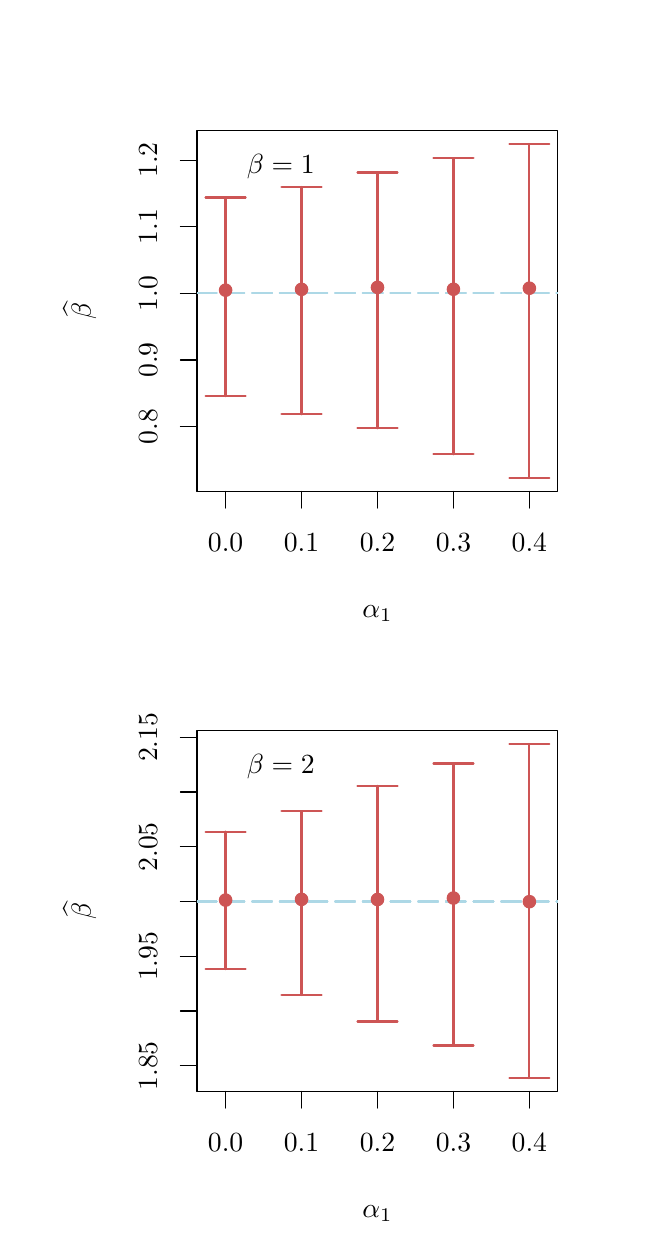
\begin{tikzpicture}[x=1pt,y=1pt]
\definecolor{fillColor}{RGB}{255,255,255}
\path[use as bounding box,fill=fillColor,fill opacity=0.00] (0,0) rectangle (216.81,433.62);
\begin{scope}
\path[clip] ( 61.20,266.01) rectangle (191.61,396.42);
\definecolor{drawColor}{RGB}{255,255,255}
\definecolor{fillColor}{RGB}{255,255,255}

\path[draw=drawColor,line width= 0.4pt,line join=round,line cap=round,fill=fillColor] ( 71.52,338.76) circle (  2.25);

\path[draw=drawColor,line width= 0.4pt,line join=round,line cap=round,fill=fillColor] ( 98.96,339.06) circle (  2.25);

\path[draw=drawColor,line width= 0.4pt,line join=round,line cap=round,fill=fillColor] (126.41,339.77) circle (  2.25);

\path[draw=drawColor,line width= 0.4pt,line join=round,line cap=round,fill=fillColor] (153.85,339.09) circle (  2.25);

\path[draw=drawColor,line width= 0.4pt,line join=round,line cap=round,fill=fillColor] (181.29,339.47) circle (  2.25);
\end{scope}
\begin{scope}
\path[clip] (  0.00,  0.00) rectangle (216.81,433.62);
\definecolor{drawColor}{RGB}{0,0,0}

\path[draw=drawColor,line width= 0.4pt,line join=round,line cap=round] ( 71.52,266.01) -- (181.29,266.01);

\path[draw=drawColor,line width= 0.4pt,line join=round,line cap=round] ( 71.52,266.01) -- ( 71.52,260.01);

\path[draw=drawColor,line width= 0.4pt,line join=round,line cap=round] ( 98.96,266.01) -- ( 98.96,260.01);

\path[draw=drawColor,line width= 0.4pt,line join=round,line cap=round] (126.41,266.01) -- (126.41,260.01);

\path[draw=drawColor,line width= 0.4pt,line join=round,line cap=round] (153.85,266.01) -- (153.85,260.01);

\path[draw=drawColor,line width= 0.4pt,line join=round,line cap=round] (181.29,266.01) -- (181.29,260.01);

\node[text=drawColor,anchor=base,inner sep=0pt, outer sep=0pt, scale=  1.00] at ( 71.52,244.41) {0.0};

\node[text=drawColor,anchor=base,inner sep=0pt, outer sep=0pt, scale=  1.00] at ( 98.96,244.41) {0.1};

\node[text=drawColor,anchor=base,inner sep=0pt, outer sep=0pt, scale=  1.00] at (126.41,244.41) {0.2};

\node[text=drawColor,anchor=base,inner sep=0pt, outer sep=0pt, scale=  1.00] at (153.85,244.41) {0.3};

\node[text=drawColor,anchor=base,inner sep=0pt, outer sep=0pt, scale=  1.00] at (181.29,244.41) {0.4};

\path[draw=drawColor,line width= 0.4pt,line join=round,line cap=round] ( 61.20,289.45) -- ( 61.20,385.76);

\path[draw=drawColor,line width= 0.4pt,line join=round,line cap=round] ( 61.20,289.45) -- ( 55.20,289.45);

\path[draw=drawColor,line width= 0.4pt,line join=round,line cap=round] ( 61.20,313.53) -- ( 55.20,313.53);

\path[draw=drawColor,line width= 0.4pt,line join=round,line cap=round] ( 61.20,337.61) -- ( 55.20,337.61);

\path[draw=drawColor,line width= 0.4pt,line join=round,line cap=round] ( 61.20,361.69) -- ( 55.20,361.69);

\path[draw=drawColor,line width= 0.4pt,line join=round,line cap=round] ( 61.20,385.76) -- ( 55.20,385.76);

\node[text=drawColor,rotate= 90.00,anchor=base,inner sep=0pt, outer sep=0pt, scale=  1.00] at ( 46.80,289.45) {0.8};

\node[text=drawColor,rotate= 90.00,anchor=base,inner sep=0pt, outer sep=0pt, scale=  1.00] at ( 46.80,313.53) {0.9};

\node[text=drawColor,rotate= 90.00,anchor=base,inner sep=0pt, outer sep=0pt, scale=  1.00] at ( 46.80,337.61) {1.0};

\node[text=drawColor,rotate= 90.00,anchor=base,inner sep=0pt, outer sep=0pt, scale=  1.00] at ( 46.80,361.69) {1.1};

\node[text=drawColor,rotate= 90.00,anchor=base,inner sep=0pt, outer sep=0pt, scale=  1.00] at ( 46.80,385.76) {1.2};

\path[draw=drawColor,line width= 0.4pt,line join=round,line cap=round] ( 61.20,266.01) --
	(191.61,266.01) --
	(191.61,396.42) --
	( 61.20,396.42) --
	( 61.20,266.01);
\end{scope}
\begin{scope}
\path[clip] (  0.00,216.81) rectangle (216.81,433.62);
\definecolor{drawColor}{RGB}{0,0,0}

\node[text=drawColor,anchor=base,inner sep=0pt, outer sep=0pt, scale=  1.00] at (126.41,220.41) {$\alpha_1$};

\node[text=drawColor,rotate= 90.00,anchor=base,inner sep=0pt, outer sep=0pt, scale=  1.00] at ( 22.80,331.22) {$\widehat{\beta}$};
\end{scope}
\begin{scope}
\path[clip] ( 61.20,266.01) rectangle (191.61,396.42);
\definecolor{drawColor}{RGB}{0,0,0}

\node[text=drawColor,anchor=base west,inner sep=0pt, outer sep=0pt, scale=  1.00] at ( 79.20,380.98) {$\beta=1$};
\definecolor{drawColor}{RGB}{173,216,230}

\path[draw=drawColor,line width= 0.8pt,dash pattern=on 7pt off 3pt ,line join=round,line cap=round] ( 61.20,337.61) -- (191.61,337.61);

\path[draw=drawColor,line width= 0.8pt,dash pattern=on 7pt off 3pt ,line join=round,line cap=round] ( 61.20,337.61) -- (191.61,337.61);

\path[draw=drawColor,line width= 0.8pt,dash pattern=on 7pt off 3pt ,line join=round,line cap=round] ( 61.20,337.61) -- (191.61,337.61);

\path[draw=drawColor,line width= 0.8pt,dash pattern=on 7pt off 3pt ,line join=round,line cap=round] ( 61.20,337.61) -- (191.61,337.61);

\path[draw=drawColor,line width= 0.8pt,dash pattern=on 7pt off 3pt ,line join=round,line cap=round] ( 61.20,337.61) -- (191.61,337.61);
\definecolor{drawColor}{RGB}{205,85,85}

\path[draw=drawColor,line width= 0.8pt,line join=round,line cap=round] ( 71.52,300.47) -- ( 71.52,372.28);

\path[draw=drawColor,line width= 0.8pt,line join=round,line cap=round] ( 64.29,300.47) --
	( 71.52,300.47) --
	( 78.75,300.47);

\path[draw=drawColor,line width= 0.8pt,line join=round,line cap=round] ( 78.75,372.28) --
	( 71.52,372.28) --
	( 64.29,372.28);

\path[draw=drawColor,line width= 0.8pt,line join=round,line cap=round] ( 98.96,293.91) -- ( 98.96,376.04);

\path[draw=drawColor,line width= 0.8pt,line join=round,line cap=round] ( 91.73,293.91) --
	( 98.96,293.91) --
	(106.19,293.91);

\path[draw=drawColor,line width= 0.8pt,line join=round,line cap=round] (106.19,376.04) --
	( 98.96,376.04) --
	( 91.73,376.04);

\path[draw=drawColor,line width= 0.8pt,line join=round,line cap=round] (126.41,288.86) -- (126.41,381.25);

\path[draw=drawColor,line width= 0.8pt,line join=round,line cap=round] (119.18,288.86) --
	(126.41,288.86) --
	(133.63,288.86);

\path[draw=drawColor,line width= 0.8pt,line join=round,line cap=round] (133.63,381.25) --
	(126.41,381.25) --
	(119.18,381.25);

\path[draw=drawColor,line width= 0.8pt,line join=round,line cap=round] (153.85,279.45) -- (153.85,386.47);

\path[draw=drawColor,line width= 0.8pt,line join=round,line cap=round] (146.62,279.45) --
	(153.85,279.45) --
	(161.08,279.45);

\path[draw=drawColor,line width= 0.8pt,line join=round,line cap=round] (161.08,386.47) --
	(153.85,386.47) --
	(146.62,386.47);

\path[draw=drawColor,line width= 0.8pt,line join=round,line cap=round] (181.29,270.84) -- (181.29,391.59);

\path[draw=drawColor,line width= 0.8pt,line join=round,line cap=round] (174.06,270.84) --
	(181.29,270.84) --
	(188.52,270.84);

\path[draw=drawColor,line width= 0.8pt,line join=round,line cap=round] (188.52,391.59) --
	(181.29,391.59) --
	(174.06,391.59);
\definecolor{fillColor}{RGB}{205,85,85}

\path[draw=drawColor,line width= 0.4pt,line join=round,line cap=round,fill=fillColor] ( 71.52,338.76) circle (  2.25);

\path[draw=drawColor,line width= 0.4pt,line join=round,line cap=round,fill=fillColor] ( 98.96,339.06) circle (  2.25);

\path[draw=drawColor,line width= 0.4pt,line join=round,line cap=round,fill=fillColor] (126.41,339.77) circle (  2.25);

\path[draw=drawColor,line width= 0.4pt,line join=round,line cap=round,fill=fillColor] (153.85,339.09) circle (  2.25);

\path[draw=drawColor,line width= 0.4pt,line join=round,line cap=round,fill=fillColor] (181.29,339.47) circle (  2.25);
\end{scope}
\begin{scope}
\path[clip] ( 61.20, 49.20) rectangle (191.61,179.61);
\definecolor{drawColor}{RGB}{255,255,255}
\definecolor{fillColor}{RGB}{255,255,255}

\path[draw=drawColor,line width= 0.4pt,line join=round,line cap=round,fill=fillColor] ( 71.52,118.37) circle (  2.25);

\path[draw=drawColor,line width= 0.4pt,line join=round,line cap=round,fill=fillColor] ( 98.96,118.63) circle (  2.25);

\path[draw=drawColor,line width= 0.4pt,line join=round,line cap=round,fill=fillColor] (126.41,118.58) circle (  2.25);

\path[draw=drawColor,line width= 0.4pt,line join=round,line cap=round,fill=fillColor] (153.85,119.11) circle (  2.25);

\path[draw=drawColor,line width= 0.4pt,line join=round,line cap=round,fill=fillColor] (181.29,117.80) circle (  2.25);
\end{scope}
\begin{scope}
\path[clip] (  0.00,  0.00) rectangle (216.81,433.62);
\definecolor{drawColor}{RGB}{0,0,0}

\path[draw=drawColor,line width= 0.4pt,line join=round,line cap=round] ( 71.52, 49.20) -- (181.29, 49.20);

\path[draw=drawColor,line width= 0.4pt,line join=round,line cap=round] ( 71.52, 49.20) -- ( 71.52, 43.20);

\path[draw=drawColor,line width= 0.4pt,line join=round,line cap=round] ( 98.96, 49.20) -- ( 98.96, 43.20);

\path[draw=drawColor,line width= 0.4pt,line join=round,line cap=round] (126.41, 49.20) -- (126.41, 43.20);

\path[draw=drawColor,line width= 0.4pt,line join=round,line cap=round] (153.85, 49.20) -- (153.85, 43.20);

\path[draw=drawColor,line width= 0.4pt,line join=round,line cap=round] (181.29, 49.20) -- (181.29, 43.20);

\node[text=drawColor,anchor=base,inner sep=0pt, outer sep=0pt, scale=  1.00] at ( 71.52, 27.60) {0.0};

\node[text=drawColor,anchor=base,inner sep=0pt, outer sep=0pt, scale=  1.00] at ( 98.96, 27.60) {0.1};

\node[text=drawColor,anchor=base,inner sep=0pt, outer sep=0pt, scale=  1.00] at (126.41, 27.60) {0.2};

\node[text=drawColor,anchor=base,inner sep=0pt, outer sep=0pt, scale=  1.00] at (153.85, 27.60) {0.3};

\node[text=drawColor,anchor=base,inner sep=0pt, outer sep=0pt, scale=  1.00] at (181.29, 27.60) {0.4};

\path[draw=drawColor,line width= 0.4pt,line join=round,line cap=round] ( 61.20, 58.49) -- ( 61.20,177.20);

\path[draw=drawColor,line width= 0.4pt,line join=round,line cap=round] ( 61.20, 58.49) -- ( 55.20, 58.49);

\path[draw=drawColor,line width= 0.4pt,line join=round,line cap=round] ( 61.20, 78.28) -- ( 55.20, 78.28);

\path[draw=drawColor,line width= 0.4pt,line join=round,line cap=round] ( 61.20, 98.06) -- ( 55.20, 98.06);

\path[draw=drawColor,line width= 0.4pt,line join=round,line cap=round] ( 61.20,117.85) -- ( 55.20,117.85);

\path[draw=drawColor,line width= 0.4pt,line join=round,line cap=round] ( 61.20,137.63) -- ( 55.20,137.63);

\path[draw=drawColor,line width= 0.4pt,line join=round,line cap=round] ( 61.20,157.41) -- ( 55.20,157.41);

\path[draw=drawColor,line width= 0.4pt,line join=round,line cap=round] ( 61.20,177.20) -- ( 55.20,177.20);

\node[text=drawColor,rotate= 90.00,anchor=base,inner sep=0pt, outer sep=0pt, scale=  1.00] at ( 46.80, 58.49) {1.85};

\node[text=drawColor,rotate= 90.00,anchor=base,inner sep=0pt, outer sep=0pt, scale=  1.00] at ( 46.80, 98.06) {1.95};

\node[text=drawColor,rotate= 90.00,anchor=base,inner sep=0pt, outer sep=0pt, scale=  1.00] at ( 46.80,137.63) {2.05};

\node[text=drawColor,rotate= 90.00,anchor=base,inner sep=0pt, outer sep=0pt, scale=  1.00] at ( 46.80,177.20) {2.15};

\path[draw=drawColor,line width= 0.4pt,line join=round,line cap=round] ( 61.20, 49.20) --
	(191.61, 49.20) --
	(191.61,179.61) --
	( 61.20,179.61) --
	( 61.20, 49.20);
\end{scope}
\begin{scope}
\path[clip] (  0.00,  0.00) rectangle (216.81,216.81);
\definecolor{drawColor}{RGB}{0,0,0}

\node[text=drawColor,anchor=base,inner sep=0pt, outer sep=0pt, scale=  1.00] at (126.41,  3.60) {$\alpha_1$};

\node[text=drawColor,rotate= 90.00,anchor=base,inner sep=0pt, outer sep=0pt, scale=  1.00] at ( 22.80,114.41) {$\widehat{\beta}$};
\end{scope}
\begin{scope}
\path[clip] ( 61.20, 49.20) rectangle (191.61,179.61);
\definecolor{drawColor}{RGB}{0,0,0}

\node[text=drawColor,anchor=base west,inner sep=0pt, outer sep=0pt, scale=  1.00] at ( 79.20,164.17) {$\beta=2$};
\definecolor{drawColor}{RGB}{173,216,230}

\path[draw=drawColor,line width= 0.8pt,dash pattern=on 7pt off 3pt ,line join=round,line cap=round] ( 61.20,117.85) -- (191.61,117.85);

\path[draw=drawColor,line width= 0.8pt,dash pattern=on 7pt off 3pt ,line join=round,line cap=round] ( 61.20,117.85) -- (191.61,117.85);

\path[draw=drawColor,line width= 0.8pt,dash pattern=on 7pt off 3pt ,line join=round,line cap=round] ( 61.20,117.85) -- (191.61,117.85);

\path[draw=drawColor,line width= 0.8pt,dash pattern=on 7pt off 3pt ,line join=round,line cap=round] ( 61.20,117.85) -- (191.61,117.85);

\path[draw=drawColor,line width= 0.8pt,dash pattern=on 7pt off 3pt ,line join=round,line cap=round] ( 61.20,117.85) -- (191.61,117.85);
\definecolor{drawColor}{RGB}{205,85,85}

\path[draw=drawColor,line width= 0.8pt,line join=round,line cap=round] ( 71.52, 93.44) -- ( 71.52,143.11);

\path[draw=drawColor,line width= 0.8pt,line join=round,line cap=round] ( 64.29, 93.44) --
	( 71.52, 93.44) --
	( 78.75, 93.44);

\path[draw=drawColor,line width= 0.8pt,line join=round,line cap=round] ( 78.75,143.11) --
	( 71.52,143.11) --
	( 64.29,143.11);

\path[draw=drawColor,line width= 0.8pt,line join=round,line cap=round] ( 98.96, 84.05) -- ( 98.96,150.43);

\path[draw=drawColor,line width= 0.8pt,line join=round,line cap=round] ( 91.73, 84.05) --
	( 98.96, 84.05) --
	(106.19, 84.05);

\path[draw=drawColor,line width= 0.8pt,line join=round,line cap=round] (106.19,150.43) --
	( 98.96,150.43) --
	( 91.73,150.43);

\path[draw=drawColor,line width= 0.8pt,line join=round,line cap=round] (126.41, 74.47) -- (126.41,159.63);

\path[draw=drawColor,line width= 0.8pt,line join=round,line cap=round] (119.18, 74.47) --
	(126.41, 74.47) --
	(133.63, 74.47);

\path[draw=drawColor,line width= 0.8pt,line join=round,line cap=round] (133.63,159.63) --
	(126.41,159.63) --
	(119.18,159.63);

\path[draw=drawColor,line width= 0.8pt,line join=round,line cap=round] (153.85, 65.82) -- (153.85,167.70);

\path[draw=drawColor,line width= 0.8pt,line join=round,line cap=round] (146.62, 65.82) --
	(153.85, 65.82) --
	(161.08, 65.82);

\path[draw=drawColor,line width= 0.8pt,line join=round,line cap=round] (161.08,167.70) --
	(153.85,167.70) --
	(146.62,167.70);

\path[draw=drawColor,line width= 0.8pt,line join=round,line cap=round] (181.29, 54.03) -- (181.29,174.78);

\path[draw=drawColor,line width= 0.8pt,line join=round,line cap=round] (174.06, 54.03) --
	(181.29, 54.03) --
	(188.52, 54.03);

\path[draw=drawColor,line width= 0.8pt,line join=round,line cap=round] (188.52,174.78) --
	(181.29,174.78) --
	(174.06,174.78);
\definecolor{fillColor}{RGB}{205,85,85}

\path[draw=drawColor,line width= 0.4pt,line join=round,line cap=round,fill=fillColor] ( 71.52,118.37) circle (  2.25);

\path[draw=drawColor,line width= 0.4pt,line join=round,line cap=round,fill=fillColor] ( 98.96,118.63) circle (  2.25);

\path[draw=drawColor,line width= 0.4pt,line join=round,line cap=round,fill=fillColor] (126.41,118.58) circle (  2.25);

\path[draw=drawColor,line width= 0.4pt,line join=round,line cap=round,fill=fillColor] (153.85,119.11) circle (  2.25);

\path[draw=drawColor,line width= 0.4pt,line join=round,line cap=round,fill=fillColor] (181.29,117.80) circle (  2.25);
\end{scope}
\end{tikzpicture}

%  \end{subfigure}
%\endgroup
%\end{figure}
%\end{frame}
%
%%%%%%%%%%%%%%%%%%%%%%%%%%%%%%%%%%%%%%
%\begin{frame}
%\begin{figure}[h]
%  \scriptsize
%  \begingroup
%  \tikzset{every picture/.style={scale=0.53}}
%  \centering
%  \begin{subfigure}[b]{0.31\textwidth}
%\caption{\footnotesize $N=500, \delta = 0.2$}
%  % Created by tikzDevice version 0.8.1 on 2015-11-17 12:15:23
% !TEX encoding = UTF-8 Unicode
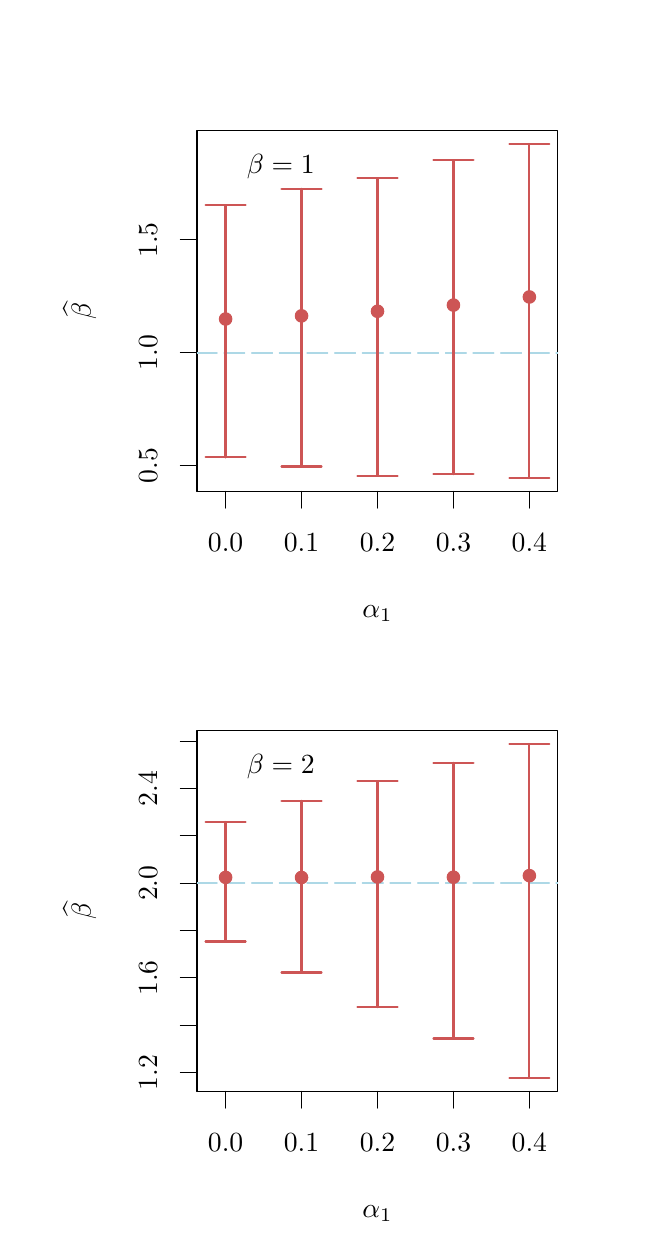
\begin{tikzpicture}[x=1pt,y=1pt]
\definecolor{fillColor}{RGB}{255,255,255}
\path[use as bounding box,fill=fillColor,fill opacity=0.00] (0,0) rectangle (216.81,433.62);
\begin{scope}
\path[clip] ( 61.20,266.01) rectangle (191.61,396.42);
\definecolor{drawColor}{RGB}{255,255,255}
\definecolor{fillColor}{RGB}{255,255,255}

\path[draw=drawColor,line width= 0.4pt,line join=round,line cap=round,fill=fillColor] ( 71.52,328.34) circle (  2.25);

\path[draw=drawColor,line width= 0.4pt,line join=round,line cap=round,fill=fillColor] ( 98.96,329.48) circle (  2.25);

\path[draw=drawColor,line width= 0.4pt,line join=round,line cap=round,fill=fillColor] (126.41,331.14) circle (  2.25);

\path[draw=drawColor,line width= 0.4pt,line join=round,line cap=round,fill=fillColor] (153.85,333.37) circle (  2.25);

\path[draw=drawColor,line width= 0.4pt,line join=round,line cap=round,fill=fillColor] (181.29,336.31) circle (  2.25);
\end{scope}
\begin{scope}
\path[clip] (  0.00,  0.00) rectangle (216.81,433.62);
\definecolor{drawColor}{RGB}{0,0,0}

\path[draw=drawColor,line width= 0.4pt,line join=round,line cap=round] ( 71.52,266.01) -- (181.29,266.01);

\path[draw=drawColor,line width= 0.4pt,line join=round,line cap=round] ( 71.52,266.01) -- ( 71.52,260.01);

\path[draw=drawColor,line width= 0.4pt,line join=round,line cap=round] ( 98.96,266.01) -- ( 98.96,260.01);

\path[draw=drawColor,line width= 0.4pt,line join=round,line cap=round] (126.41,266.01) -- (126.41,260.01);

\path[draw=drawColor,line width= 0.4pt,line join=round,line cap=round] (153.85,266.01) -- (153.85,260.01);

\path[draw=drawColor,line width= 0.4pt,line join=round,line cap=round] (181.29,266.01) -- (181.29,260.01);

\node[text=drawColor,anchor=base,inner sep=0pt, outer sep=0pt, scale=  1.00] at ( 71.52,244.41) {0.0};

\node[text=drawColor,anchor=base,inner sep=0pt, outer sep=0pt, scale=  1.00] at ( 98.96,244.41) {0.1};

\node[text=drawColor,anchor=base,inner sep=0pt, outer sep=0pt, scale=  1.00] at (126.41,244.41) {0.2};

\node[text=drawColor,anchor=base,inner sep=0pt, outer sep=0pt, scale=  1.00] at (153.85,244.41) {0.3};

\node[text=drawColor,anchor=base,inner sep=0pt, outer sep=0pt, scale=  1.00] at (181.29,244.41) {0.4};

\path[draw=drawColor,line width= 0.4pt,line join=round,line cap=round] ( 61.20,275.35) -- ( 61.20,356.94);

\path[draw=drawColor,line width= 0.4pt,line join=round,line cap=round] ( 61.20,275.35) -- ( 55.20,275.35);

\path[draw=drawColor,line width= 0.4pt,line join=round,line cap=round] ( 61.20,316.14) -- ( 55.20,316.14);

\path[draw=drawColor,line width= 0.4pt,line join=round,line cap=round] ( 61.20,356.94) -- ( 55.20,356.94);

\node[text=drawColor,rotate= 90.00,anchor=base,inner sep=0pt, outer sep=0pt, scale=  1.00] at ( 46.80,275.35) {0.5};

\node[text=drawColor,rotate= 90.00,anchor=base,inner sep=0pt, outer sep=0pt, scale=  1.00] at ( 46.80,316.14) {1.0};

\node[text=drawColor,rotate= 90.00,anchor=base,inner sep=0pt, outer sep=0pt, scale=  1.00] at ( 46.80,356.94) {1.5};

\path[draw=drawColor,line width= 0.4pt,line join=round,line cap=round] ( 61.20,266.01) --
	(191.61,266.01) --
	(191.61,396.42) --
	( 61.20,396.42) --
	( 61.20,266.01);
\end{scope}
\begin{scope}
\path[clip] (  0.00,216.81) rectangle (216.81,433.62);
\definecolor{drawColor}{RGB}{0,0,0}

\node[text=drawColor,anchor=base,inner sep=0pt, outer sep=0pt, scale=  1.00] at (126.41,220.41) {$\alpha_1$};

\node[text=drawColor,rotate= 90.00,anchor=base,inner sep=0pt, outer sep=0pt, scale=  1.00] at ( 22.80,331.22) {$\widehat{\beta}$};
\end{scope}
\begin{scope}
\path[clip] ( 61.20,266.01) rectangle (191.61,396.42);
\definecolor{drawColor}{RGB}{0,0,0}

\node[text=drawColor,anchor=base west,inner sep=0pt, outer sep=0pt, scale=  1.00] at ( 79.20,380.98) {$\beta=1$};
\definecolor{drawColor}{RGB}{173,216,230}

\path[draw=drawColor,line width= 0.8pt,dash pattern=on 7pt off 3pt ,line join=round,line cap=round] ( 61.20,316.14) -- (191.61,316.14);

\path[draw=drawColor,line width= 0.8pt,dash pattern=on 7pt off 3pt ,line join=round,line cap=round] ( 61.20,316.14) -- (191.61,316.14);

\path[draw=drawColor,line width= 0.8pt,dash pattern=on 7pt off 3pt ,line join=round,line cap=round] ( 61.20,316.14) -- (191.61,316.14);

\path[draw=drawColor,line width= 0.8pt,dash pattern=on 7pt off 3pt ,line join=round,line cap=round] ( 61.20,316.14) -- (191.61,316.14);

\path[draw=drawColor,line width= 0.8pt,dash pattern=on 7pt off 3pt ,line join=round,line cap=round] ( 61.20,316.14) -- (191.61,316.14);
\definecolor{drawColor}{RGB}{205,85,85}

\path[draw=drawColor,line width= 0.8pt,line join=round,line cap=round] ( 71.52,278.34) -- ( 71.52,369.48);

\path[draw=drawColor,line width= 0.8pt,line join=round,line cap=round] ( 64.29,278.34) --
	( 71.52,278.34) --
	( 78.75,278.34);

\path[draw=drawColor,line width= 0.8pt,line join=round,line cap=round] ( 78.75,369.48) --
	( 71.52,369.48) --
	( 64.29,369.48);

\path[draw=drawColor,line width= 0.8pt,line join=round,line cap=round] ( 98.96,275.02) -- ( 98.96,375.35);

\path[draw=drawColor,line width= 0.8pt,line join=round,line cap=round] ( 91.73,275.02) --
	( 98.96,275.02) --
	(106.19,275.02);

\path[draw=drawColor,line width= 0.8pt,line join=round,line cap=round] (106.19,375.35) --
	( 98.96,375.35) --
	( 91.73,375.35);

\path[draw=drawColor,line width= 0.8pt,line join=round,line cap=round] (126.41,271.75) -- (126.41,379.21);

\path[draw=drawColor,line width= 0.8pt,line join=round,line cap=round] (119.18,271.75) --
	(126.41,271.75) --
	(133.63,271.75);

\path[draw=drawColor,line width= 0.8pt,line join=round,line cap=round] (133.63,379.21) --
	(126.41,379.21) --
	(119.18,379.21);

\path[draw=drawColor,line width= 0.8pt,line join=round,line cap=round] (153.85,272.29) -- (153.85,385.66);

\path[draw=drawColor,line width= 0.8pt,line join=round,line cap=round] (146.62,272.29) --
	(153.85,272.29) --
	(161.08,272.29);

\path[draw=drawColor,line width= 0.8pt,line join=round,line cap=round] (161.08,385.66) --
	(153.85,385.66) --
	(146.62,385.66);

\path[draw=drawColor,line width= 0.8pt,line join=round,line cap=round] (181.29,270.84) -- (181.29,391.59);

\path[draw=drawColor,line width= 0.8pt,line join=round,line cap=round] (174.06,270.84) --
	(181.29,270.84) --
	(188.52,270.84);

\path[draw=drawColor,line width= 0.8pt,line join=round,line cap=round] (188.52,391.59) --
	(181.29,391.59) --
	(174.06,391.59);
\definecolor{fillColor}{RGB}{205,85,85}

\path[draw=drawColor,line width= 0.4pt,line join=round,line cap=round,fill=fillColor] ( 71.52,328.34) circle (  2.25);

\path[draw=drawColor,line width= 0.4pt,line join=round,line cap=round,fill=fillColor] ( 98.96,329.48) circle (  2.25);

\path[draw=drawColor,line width= 0.4pt,line join=round,line cap=round,fill=fillColor] (126.41,331.14) circle (  2.25);

\path[draw=drawColor,line width= 0.4pt,line join=round,line cap=round,fill=fillColor] (153.85,333.37) circle (  2.25);

\path[draw=drawColor,line width= 0.4pt,line join=round,line cap=round,fill=fillColor] (181.29,336.31) circle (  2.25);
\end{scope}
\begin{scope}
\path[clip] ( 61.20, 49.20) rectangle (191.61,179.61);
\definecolor{drawColor}{RGB}{255,255,255}
\definecolor{fillColor}{RGB}{255,255,255}

\path[draw=drawColor,line width= 0.4pt,line join=round,line cap=round,fill=fillColor] ( 71.52,126.58) circle (  2.25);

\path[draw=drawColor,line width= 0.4pt,line join=round,line cap=round,fill=fillColor] ( 98.96,126.54) circle (  2.25);

\path[draw=drawColor,line width= 0.4pt,line join=round,line cap=round,fill=fillColor] (126.41,126.72) circle (  2.25);

\path[draw=drawColor,line width= 0.4pt,line join=round,line cap=round,fill=fillColor] (153.85,126.64) circle (  2.25);

\path[draw=drawColor,line width= 0.4pt,line join=round,line cap=round,fill=fillColor] (181.29,127.20) circle (  2.25);
\end{scope}
\begin{scope}
\path[clip] (  0.00,  0.00) rectangle (216.81,433.62);
\definecolor{drawColor}{RGB}{0,0,0}

\path[draw=drawColor,line width= 0.4pt,line join=round,line cap=round] ( 71.52, 49.20) -- (181.29, 49.20);

\path[draw=drawColor,line width= 0.4pt,line join=round,line cap=round] ( 71.52, 49.20) -- ( 71.52, 43.20);

\path[draw=drawColor,line width= 0.4pt,line join=round,line cap=round] ( 98.96, 49.20) -- ( 98.96, 43.20);

\path[draw=drawColor,line width= 0.4pt,line join=round,line cap=round] (126.41, 49.20) -- (126.41, 43.20);

\path[draw=drawColor,line width= 0.4pt,line join=round,line cap=round] (153.85, 49.20) -- (153.85, 43.20);

\path[draw=drawColor,line width= 0.4pt,line join=round,line cap=round] (181.29, 49.20) -- (181.29, 43.20);

\node[text=drawColor,anchor=base,inner sep=0pt, outer sep=0pt, scale=  1.00] at ( 71.52, 27.60) {0.0};

\node[text=drawColor,anchor=base,inner sep=0pt, outer sep=0pt, scale=  1.00] at ( 98.96, 27.60) {0.1};

\node[text=drawColor,anchor=base,inner sep=0pt, outer sep=0pt, scale=  1.00] at (126.41, 27.60) {0.2};

\node[text=drawColor,anchor=base,inner sep=0pt, outer sep=0pt, scale=  1.00] at (153.85, 27.60) {0.3};

\node[text=drawColor,anchor=base,inner sep=0pt, outer sep=0pt, scale=  1.00] at (181.29, 27.60) {0.4};

\path[draw=drawColor,line width= 0.4pt,line join=round,line cap=round] ( 61.20, 56.06) -- ( 61.20,175.78);

\path[draw=drawColor,line width= 0.4pt,line join=round,line cap=round] ( 61.20, 56.06) -- ( 55.20, 56.06);

\path[draw=drawColor,line width= 0.4pt,line join=round,line cap=round] ( 61.20, 73.16) -- ( 55.20, 73.16);

\path[draw=drawColor,line width= 0.4pt,line join=round,line cap=round] ( 61.20, 90.26) -- ( 55.20, 90.26);

\path[draw=drawColor,line width= 0.4pt,line join=round,line cap=round] ( 61.20,107.37) -- ( 55.20,107.37);

\path[draw=drawColor,line width= 0.4pt,line join=round,line cap=round] ( 61.20,124.47) -- ( 55.20,124.47);

\path[draw=drawColor,line width= 0.4pt,line join=round,line cap=round] ( 61.20,141.58) -- ( 55.20,141.58);

\path[draw=drawColor,line width= 0.4pt,line join=round,line cap=round] ( 61.20,158.68) -- ( 55.20,158.68);

\path[draw=drawColor,line width= 0.4pt,line join=round,line cap=round] ( 61.20,175.78) -- ( 55.20,175.78);

\node[text=drawColor,rotate= 90.00,anchor=base,inner sep=0pt, outer sep=0pt, scale=  1.00] at ( 46.80, 56.06) {1.2};

\node[text=drawColor,rotate= 90.00,anchor=base,inner sep=0pt, outer sep=0pt, scale=  1.00] at ( 46.80, 90.26) {1.6};

\node[text=drawColor,rotate= 90.00,anchor=base,inner sep=0pt, outer sep=0pt, scale=  1.00] at ( 46.80,124.47) {2.0};

\node[text=drawColor,rotate= 90.00,anchor=base,inner sep=0pt, outer sep=0pt, scale=  1.00] at ( 46.80,158.68) {2.4};

\path[draw=drawColor,line width= 0.4pt,line join=round,line cap=round] ( 61.20, 49.20) --
	(191.61, 49.20) --
	(191.61,179.61) --
	( 61.20,179.61) --
	( 61.20, 49.20);
\end{scope}
\begin{scope}
\path[clip] (  0.00,  0.00) rectangle (216.81,216.81);
\definecolor{drawColor}{RGB}{0,0,0}

\node[text=drawColor,anchor=base,inner sep=0pt, outer sep=0pt, scale=  1.00] at (126.41,  3.60) {$\alpha_1$};

\node[text=drawColor,rotate= 90.00,anchor=base,inner sep=0pt, outer sep=0pt, scale=  1.00] at ( 22.80,114.41) {$\widehat{\beta}$};
\end{scope}
\begin{scope}
\path[clip] ( 61.20, 49.20) rectangle (191.61,179.61);
\definecolor{drawColor}{RGB}{0,0,0}

\node[text=drawColor,anchor=base west,inner sep=0pt, outer sep=0pt, scale=  1.00] at ( 79.20,164.17) {$\beta=2$};
\definecolor{drawColor}{RGB}{173,216,230}

\path[draw=drawColor,line width= 0.8pt,dash pattern=on 7pt off 3pt ,line join=round,line cap=round] ( 61.20,124.47) -- (191.61,124.47);

\path[draw=drawColor,line width= 0.8pt,dash pattern=on 7pt off 3pt ,line join=round,line cap=round] ( 61.20,124.47) -- (191.61,124.47);

\path[draw=drawColor,line width= 0.8pt,dash pattern=on 7pt off 3pt ,line join=round,line cap=round] ( 61.20,124.47) -- (191.61,124.47);

\path[draw=drawColor,line width= 0.8pt,dash pattern=on 7pt off 3pt ,line join=round,line cap=round] ( 61.20,124.47) -- (191.61,124.47);

\path[draw=drawColor,line width= 0.8pt,dash pattern=on 7pt off 3pt ,line join=round,line cap=round] ( 61.20,124.47) -- (191.61,124.47);
\definecolor{drawColor}{RGB}{205,85,85}

\path[draw=drawColor,line width= 0.8pt,line join=round,line cap=round] ( 71.52,103.38) -- ( 71.52,146.61);

\path[draw=drawColor,line width= 0.8pt,line join=round,line cap=round] ( 64.29,103.38) --
	( 71.52,103.38) --
	( 78.75,103.38);

\path[draw=drawColor,line width= 0.8pt,line join=round,line cap=round] ( 78.75,146.61) --
	( 71.52,146.61) --
	( 64.29,146.61);

\path[draw=drawColor,line width= 0.8pt,line join=round,line cap=round] ( 98.96, 92.24) -- ( 98.96,154.22);

\path[draw=drawColor,line width= 0.8pt,line join=round,line cap=round] ( 91.73, 92.24) --
	( 98.96, 92.24) --
	(106.19, 92.24);

\path[draw=drawColor,line width= 0.8pt,line join=round,line cap=round] (106.19,154.22) --
	( 98.96,154.22) --
	( 91.73,154.22);

\path[draw=drawColor,line width= 0.8pt,line join=round,line cap=round] (126.41, 79.70) -- (126.41,161.30);

\path[draw=drawColor,line width= 0.8pt,line join=round,line cap=round] (119.18, 79.70) --
	(126.41, 79.70) --
	(133.63, 79.70);

\path[draw=drawColor,line width= 0.8pt,line join=round,line cap=round] (133.63,161.30) --
	(126.41,161.30) --
	(119.18,161.30);

\path[draw=drawColor,line width= 0.8pt,line join=round,line cap=round] (153.85, 68.32) -- (153.85,167.95);

\path[draw=drawColor,line width= 0.8pt,line join=round,line cap=round] (146.62, 68.32) --
	(153.85, 68.32) --
	(161.08, 68.32);

\path[draw=drawColor,line width= 0.8pt,line join=round,line cap=round] (161.08,167.95) --
	(153.85,167.95) --
	(146.62,167.95);

\path[draw=drawColor,line width= 0.8pt,line join=round,line cap=round] (181.29, 54.03) -- (181.29,174.78);

\path[draw=drawColor,line width= 0.8pt,line join=round,line cap=round] (174.06, 54.03) --
	(181.29, 54.03) --
	(188.52, 54.03);

\path[draw=drawColor,line width= 0.8pt,line join=round,line cap=round] (188.52,174.78) --
	(181.29,174.78) --
	(174.06,174.78);
\definecolor{fillColor}{RGB}{205,85,85}

\path[draw=drawColor,line width= 0.4pt,line join=round,line cap=round,fill=fillColor] ( 71.52,126.58) circle (  2.25);

\path[draw=drawColor,line width= 0.4pt,line join=round,line cap=round,fill=fillColor] ( 98.96,126.54) circle (  2.25);

\path[draw=drawColor,line width= 0.4pt,line join=round,line cap=round,fill=fillColor] (126.41,126.72) circle (  2.25);

\path[draw=drawColor,line width= 0.4pt,line join=round,line cap=round,fill=fillColor] (153.85,126.64) circle (  2.25);

\path[draw=drawColor,line width= 0.4pt,line join=round,line cap=round,fill=fillColor] (181.29,127.20) circle (  2.25);
\end{scope}
\end{tikzpicture}

%  \end{subfigure}
%  ~
%  \begin{subfigure}[b]{0.31\textwidth}
%    \caption{\footnotesize $N=1000, \delta = 0.2$} 
%  % Created by tikzDevice version 0.8.1 on 2015-11-17 12:26:03
% !TEX encoding = UTF-8 Unicode
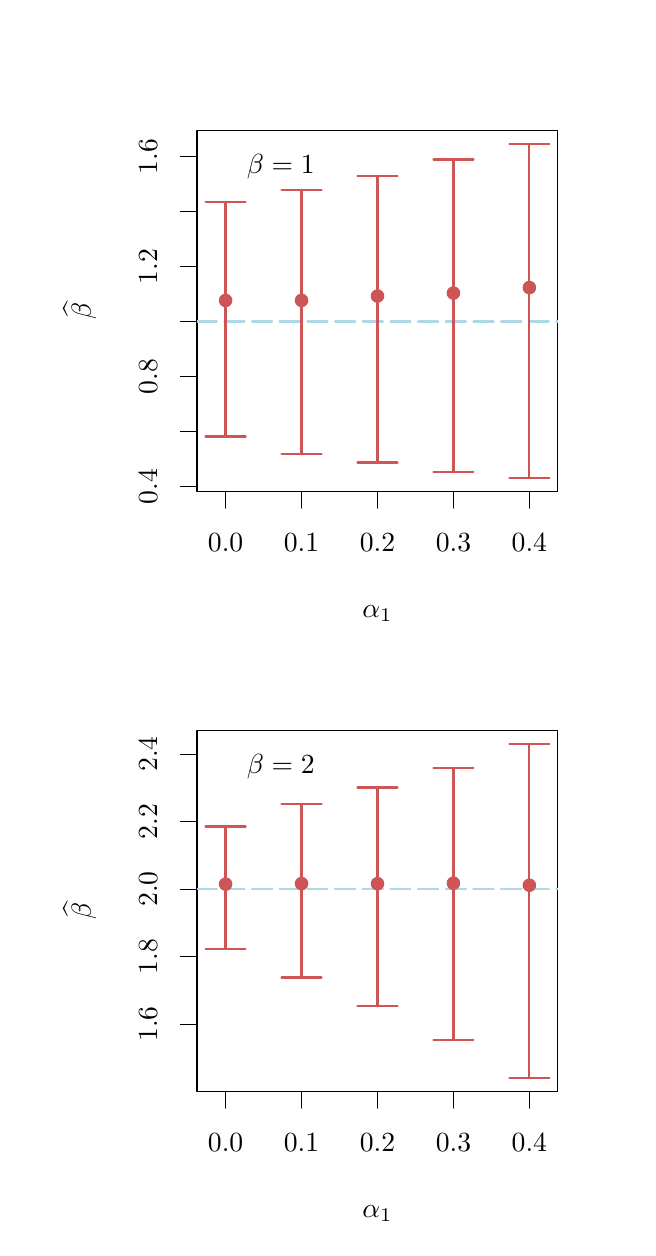
\begin{tikzpicture}[x=1pt,y=1pt]
\definecolor{fillColor}{RGB}{255,255,255}
\path[use as bounding box,fill=fillColor,fill opacity=0.00] (0,0) rectangle (216.81,433.62);
\begin{scope}
\path[clip] ( 61.20,266.01) rectangle (191.61,396.42);
\definecolor{drawColor}{RGB}{255,255,255}
\definecolor{fillColor}{RGB}{255,255,255}

\path[draw=drawColor,line width= 0.4pt,line join=round,line cap=round,fill=fillColor] ( 71.52,335.05) circle (  2.25);

\path[draw=drawColor,line width= 0.4pt,line join=round,line cap=round,fill=fillColor] ( 98.96,335.07) circle (  2.25);

\path[draw=drawColor,line width= 0.4pt,line join=round,line cap=round,fill=fillColor] (126.41,336.65) circle (  2.25);

\path[draw=drawColor,line width= 0.4pt,line join=round,line cap=round,fill=fillColor] (153.85,337.71) circle (  2.25);

\path[draw=drawColor,line width= 0.4pt,line join=round,line cap=round,fill=fillColor] (181.29,339.70) circle (  2.25);
\end{scope}
\begin{scope}
\path[clip] (  0.00,  0.00) rectangle (216.81,433.62);
\definecolor{drawColor}{RGB}{0,0,0}

\path[draw=drawColor,line width= 0.4pt,line join=round,line cap=round] ( 71.52,266.01) -- (181.29,266.01);

\path[draw=drawColor,line width= 0.4pt,line join=round,line cap=round] ( 71.52,266.01) -- ( 71.52,260.01);

\path[draw=drawColor,line width= 0.4pt,line join=round,line cap=round] ( 98.96,266.01) -- ( 98.96,260.01);

\path[draw=drawColor,line width= 0.4pt,line join=round,line cap=round] (126.41,266.01) -- (126.41,260.01);

\path[draw=drawColor,line width= 0.4pt,line join=round,line cap=round] (153.85,266.01) -- (153.85,260.01);

\path[draw=drawColor,line width= 0.4pt,line join=round,line cap=round] (181.29,266.01) -- (181.29,260.01);

\node[text=drawColor,anchor=base,inner sep=0pt, outer sep=0pt, scale=  1.00] at ( 71.52,244.41) {0.0};

\node[text=drawColor,anchor=base,inner sep=0pt, outer sep=0pt, scale=  1.00] at ( 98.96,244.41) {0.1};

\node[text=drawColor,anchor=base,inner sep=0pt, outer sep=0pt, scale=  1.00] at (126.41,244.41) {0.2};

\node[text=drawColor,anchor=base,inner sep=0pt, outer sep=0pt, scale=  1.00] at (153.85,244.41) {0.3};

\node[text=drawColor,anchor=base,inner sep=0pt, outer sep=0pt, scale=  1.00] at (181.29,244.41) {0.4};

\path[draw=drawColor,line width= 0.4pt,line join=round,line cap=round] ( 61.20,267.81) -- ( 61.20,387.00);

\path[draw=drawColor,line width= 0.4pt,line join=round,line cap=round] ( 61.20,267.81) -- ( 55.20,267.81);

\path[draw=drawColor,line width= 0.4pt,line join=round,line cap=round] ( 61.20,287.68) -- ( 55.20,287.68);

\path[draw=drawColor,line width= 0.4pt,line join=round,line cap=round] ( 61.20,307.54) -- ( 55.20,307.54);

\path[draw=drawColor,line width= 0.4pt,line join=round,line cap=round] ( 61.20,327.41) -- ( 55.20,327.41);

\path[draw=drawColor,line width= 0.4pt,line join=round,line cap=round] ( 61.20,347.27) -- ( 55.20,347.27);

\path[draw=drawColor,line width= 0.4pt,line join=round,line cap=round] ( 61.20,367.14) -- ( 55.20,367.14);

\path[draw=drawColor,line width= 0.4pt,line join=round,line cap=round] ( 61.20,387.00) -- ( 55.20,387.00);

\node[text=drawColor,rotate= 90.00,anchor=base,inner sep=0pt, outer sep=0pt, scale=  1.00] at ( 46.80,267.81) {0.4};

\node[text=drawColor,rotate= 90.00,anchor=base,inner sep=0pt, outer sep=0pt, scale=  1.00] at ( 46.80,307.54) {0.8};

\node[text=drawColor,rotate= 90.00,anchor=base,inner sep=0pt, outer sep=0pt, scale=  1.00] at ( 46.80,347.27) {1.2};

\node[text=drawColor,rotate= 90.00,anchor=base,inner sep=0pt, outer sep=0pt, scale=  1.00] at ( 46.80,387.00) {1.6};

\path[draw=drawColor,line width= 0.4pt,line join=round,line cap=round] ( 61.20,266.01) --
	(191.61,266.01) --
	(191.61,396.42) --
	( 61.20,396.42) --
	( 61.20,266.01);
\end{scope}
\begin{scope}
\path[clip] (  0.00,216.81) rectangle (216.81,433.62);
\definecolor{drawColor}{RGB}{0,0,0}

\node[text=drawColor,anchor=base,inner sep=0pt, outer sep=0pt, scale=  1.00] at (126.41,220.41) {$\alpha_1$};

\node[text=drawColor,rotate= 90.00,anchor=base,inner sep=0pt, outer sep=0pt, scale=  1.00] at ( 22.80,331.22) {$\widehat{\beta}$};
\end{scope}
\begin{scope}
\path[clip] ( 61.20,266.01) rectangle (191.61,396.42);
\definecolor{drawColor}{RGB}{0,0,0}

\node[text=drawColor,anchor=base west,inner sep=0pt, outer sep=0pt, scale=  1.00] at ( 79.20,380.98) {$\beta=1$};
\definecolor{drawColor}{RGB}{173,216,230}

\path[draw=drawColor,line width= 0.8pt,dash pattern=on 7pt off 3pt ,line join=round,line cap=round] ( 61.20,327.41) -- (191.61,327.41);

\path[draw=drawColor,line width= 0.8pt,dash pattern=on 7pt off 3pt ,line join=round,line cap=round] ( 61.20,327.41) -- (191.61,327.41);

\path[draw=drawColor,line width= 0.8pt,dash pattern=on 7pt off 3pt ,line join=round,line cap=round] ( 61.20,327.41) -- (191.61,327.41);

\path[draw=drawColor,line width= 0.8pt,dash pattern=on 7pt off 3pt ,line join=round,line cap=round] ( 61.20,327.41) -- (191.61,327.41);

\path[draw=drawColor,line width= 0.8pt,dash pattern=on 7pt off 3pt ,line join=round,line cap=round] ( 61.20,327.41) -- (191.61,327.41);
\definecolor{drawColor}{RGB}{205,85,85}

\path[draw=drawColor,line width= 0.8pt,line join=round,line cap=round] ( 71.52,285.87) -- ( 71.52,370.49);

\path[draw=drawColor,line width= 0.8pt,line join=round,line cap=round] ( 64.29,285.87) --
	( 71.52,285.87) --
	( 78.75,285.87);

\path[draw=drawColor,line width= 0.8pt,line join=round,line cap=round] ( 78.75,370.49) --
	( 71.52,370.49) --
	( 64.29,370.49);

\path[draw=drawColor,line width= 0.8pt,line join=round,line cap=round] ( 98.96,279.52) -- ( 98.96,375.05);

\path[draw=drawColor,line width= 0.8pt,line join=round,line cap=round] ( 91.73,279.52) --
	( 98.96,279.52) --
	(106.19,279.52);

\path[draw=drawColor,line width= 0.8pt,line join=round,line cap=round] (106.19,375.05) --
	( 98.96,375.05) --
	( 91.73,375.05);

\path[draw=drawColor,line width= 0.8pt,line join=round,line cap=round] (126.41,276.52) -- (126.41,380.04);

\path[draw=drawColor,line width= 0.8pt,line join=round,line cap=round] (119.18,276.52) --
	(126.41,276.52) --
	(133.63,276.52);

\path[draw=drawColor,line width= 0.8pt,line join=round,line cap=round] (133.63,380.04) --
	(126.41,380.04) --
	(119.18,380.04);

\path[draw=drawColor,line width= 0.8pt,line join=round,line cap=round] (153.85,272.99) -- (153.85,386.00);

\path[draw=drawColor,line width= 0.8pt,line join=round,line cap=round] (146.62,272.99) --
	(153.85,272.99) --
	(161.08,272.99);

\path[draw=drawColor,line width= 0.8pt,line join=round,line cap=round] (161.08,386.00) --
	(153.85,386.00) --
	(146.62,386.00);

\path[draw=drawColor,line width= 0.8pt,line join=round,line cap=round] (181.29,270.84) -- (181.29,391.59);

\path[draw=drawColor,line width= 0.8pt,line join=round,line cap=round] (174.06,270.84) --
	(181.29,270.84) --
	(188.52,270.84);

\path[draw=drawColor,line width= 0.8pt,line join=round,line cap=round] (188.52,391.59) --
	(181.29,391.59) --
	(174.06,391.59);
\definecolor{fillColor}{RGB}{205,85,85}

\path[draw=drawColor,line width= 0.4pt,line join=round,line cap=round,fill=fillColor] ( 71.52,335.05) circle (  2.25);

\path[draw=drawColor,line width= 0.4pt,line join=round,line cap=round,fill=fillColor] ( 98.96,335.07) circle (  2.25);

\path[draw=drawColor,line width= 0.4pt,line join=round,line cap=round,fill=fillColor] (126.41,336.65) circle (  2.25);

\path[draw=drawColor,line width= 0.4pt,line join=round,line cap=round,fill=fillColor] (153.85,337.71) circle (  2.25);

\path[draw=drawColor,line width= 0.4pt,line join=round,line cap=round,fill=fillColor] (181.29,339.70) circle (  2.25);
\end{scope}
\begin{scope}
\path[clip] ( 61.20, 49.20) rectangle (191.61,179.61);
\definecolor{drawColor}{RGB}{255,255,255}
\definecolor{fillColor}{RGB}{255,255,255}

\path[draw=drawColor,line width= 0.4pt,line join=round,line cap=round,fill=fillColor] ( 71.52,124.14) circle (  2.25);

\path[draw=drawColor,line width= 0.4pt,line join=round,line cap=round,fill=fillColor] ( 98.96,124.33) circle (  2.25);

\path[draw=drawColor,line width= 0.4pt,line join=round,line cap=round,fill=fillColor] (126.41,124.30) circle (  2.25);

\path[draw=drawColor,line width= 0.4pt,line join=round,line cap=round,fill=fillColor] (153.85,124.47) circle (  2.25);

\path[draw=drawColor,line width= 0.4pt,line join=round,line cap=round,fill=fillColor] (181.29,123.74) circle (  2.25);
\end{scope}
\begin{scope}
\path[clip] (  0.00,  0.00) rectangle (216.81,433.62);
\definecolor{drawColor}{RGB}{0,0,0}

\path[draw=drawColor,line width= 0.4pt,line join=round,line cap=round] ( 71.52, 49.20) -- (181.29, 49.20);

\path[draw=drawColor,line width= 0.4pt,line join=round,line cap=round] ( 71.52, 49.20) -- ( 71.52, 43.20);

\path[draw=drawColor,line width= 0.4pt,line join=round,line cap=round] ( 98.96, 49.20) -- ( 98.96, 43.20);

\path[draw=drawColor,line width= 0.4pt,line join=round,line cap=round] (126.41, 49.20) -- (126.41, 43.20);

\path[draw=drawColor,line width= 0.4pt,line join=round,line cap=round] (153.85, 49.20) -- (153.85, 43.20);

\path[draw=drawColor,line width= 0.4pt,line join=round,line cap=round] (181.29, 49.20) -- (181.29, 43.20);

\node[text=drawColor,anchor=base,inner sep=0pt, outer sep=0pt, scale=  1.00] at ( 71.52, 27.60) {0.0};

\node[text=drawColor,anchor=base,inner sep=0pt, outer sep=0pt, scale=  1.00] at ( 98.96, 27.60) {0.1};

\node[text=drawColor,anchor=base,inner sep=0pt, outer sep=0pt, scale=  1.00] at (126.41, 27.60) {0.2};

\node[text=drawColor,anchor=base,inner sep=0pt, outer sep=0pt, scale=  1.00] at (153.85, 27.60) {0.3};

\node[text=drawColor,anchor=base,inner sep=0pt, outer sep=0pt, scale=  1.00] at (181.29, 27.60) {0.4};

\path[draw=drawColor,line width= 0.4pt,line join=round,line cap=round] ( 61.20, 73.55) -- ( 61.20,171.13);

\path[draw=drawColor,line width= 0.4pt,line join=round,line cap=round] ( 61.20, 73.55) -- ( 55.20, 73.55);

\path[draw=drawColor,line width= 0.4pt,line join=round,line cap=round] ( 61.20, 97.95) -- ( 55.20, 97.95);

\path[draw=drawColor,line width= 0.4pt,line join=round,line cap=round] ( 61.20,122.34) -- ( 55.20,122.34);

\path[draw=drawColor,line width= 0.4pt,line join=round,line cap=round] ( 61.20,146.73) -- ( 55.20,146.73);

\path[draw=drawColor,line width= 0.4pt,line join=round,line cap=round] ( 61.20,171.13) -- ( 55.20,171.13);

\node[text=drawColor,rotate= 90.00,anchor=base,inner sep=0pt, outer sep=0pt, scale=  1.00] at ( 46.80, 73.55) {1.6};

\node[text=drawColor,rotate= 90.00,anchor=base,inner sep=0pt, outer sep=0pt, scale=  1.00] at ( 46.80, 97.95) {1.8};

\node[text=drawColor,rotate= 90.00,anchor=base,inner sep=0pt, outer sep=0pt, scale=  1.00] at ( 46.80,122.34) {2.0};

\node[text=drawColor,rotate= 90.00,anchor=base,inner sep=0pt, outer sep=0pt, scale=  1.00] at ( 46.80,146.73) {2.2};

\node[text=drawColor,rotate= 90.00,anchor=base,inner sep=0pt, outer sep=0pt, scale=  1.00] at ( 46.80,171.13) {2.4};

\path[draw=drawColor,line width= 0.4pt,line join=round,line cap=round] ( 61.20, 49.20) --
	(191.61, 49.20) --
	(191.61,179.61) --
	( 61.20,179.61) --
	( 61.20, 49.20);
\end{scope}
\begin{scope}
\path[clip] (  0.00,  0.00) rectangle (216.81,216.81);
\definecolor{drawColor}{RGB}{0,0,0}

\node[text=drawColor,anchor=base,inner sep=0pt, outer sep=0pt, scale=  1.00] at (126.41,  3.60) {$\alpha_1$};

\node[text=drawColor,rotate= 90.00,anchor=base,inner sep=0pt, outer sep=0pt, scale=  1.00] at ( 22.80,114.41) {$\widehat{\beta}$};
\end{scope}
\begin{scope}
\path[clip] ( 61.20, 49.20) rectangle (191.61,179.61);
\definecolor{drawColor}{RGB}{0,0,0}

\node[text=drawColor,anchor=base west,inner sep=0pt, outer sep=0pt, scale=  1.00] at ( 79.20,164.17) {$\beta=2$};
\definecolor{drawColor}{RGB}{173,216,230}

\path[draw=drawColor,line width= 0.8pt,dash pattern=on 7pt off 3pt ,line join=round,line cap=round] ( 61.20,122.34) -- (191.61,122.34);

\path[draw=drawColor,line width= 0.8pt,dash pattern=on 7pt off 3pt ,line join=round,line cap=round] ( 61.20,122.34) -- (191.61,122.34);

\path[draw=drawColor,line width= 0.8pt,dash pattern=on 7pt off 3pt ,line join=round,line cap=round] ( 61.20,122.34) -- (191.61,122.34);

\path[draw=drawColor,line width= 0.8pt,dash pattern=on 7pt off 3pt ,line join=round,line cap=round] ( 61.20,122.34) -- (191.61,122.34);

\path[draw=drawColor,line width= 0.8pt,dash pattern=on 7pt off 3pt ,line join=round,line cap=round] ( 61.20,122.34) -- (191.61,122.34);
\definecolor{drawColor}{RGB}{205,85,85}

\path[draw=drawColor,line width= 0.8pt,line join=round,line cap=round] ( 71.52,100.80) -- ( 71.52,144.93);

\path[draw=drawColor,line width= 0.8pt,line join=round,line cap=round] ( 64.29,100.80) --
	( 71.52,100.80) --
	( 78.75,100.80);

\path[draw=drawColor,line width= 0.8pt,line join=round,line cap=round] ( 78.75,144.93) --
	( 71.52,144.93) --
	( 64.29,144.93);

\path[draw=drawColor,line width= 0.8pt,line join=round,line cap=round] ( 98.96, 90.36) -- ( 98.96,153.00);

\path[draw=drawColor,line width= 0.8pt,line join=round,line cap=round] ( 91.73, 90.36) --
	( 98.96, 90.36) --
	(106.19, 90.36);

\path[draw=drawColor,line width= 0.8pt,line join=round,line cap=round] (106.19,153.00) --
	( 98.96,153.00) --
	( 91.73,153.00);

\path[draw=drawColor,line width= 0.8pt,line join=round,line cap=round] (126.41, 80.02) -- (126.41,159.09);

\path[draw=drawColor,line width= 0.8pt,line join=round,line cap=round] (119.18, 80.02) --
	(126.41, 80.02) --
	(133.63, 80.02);

\path[draw=drawColor,line width= 0.8pt,line join=round,line cap=round] (133.63,159.09) --
	(126.41,159.09) --
	(119.18,159.09);

\path[draw=drawColor,line width= 0.8pt,line join=round,line cap=round] (153.85, 67.78) -- (153.85,166.05);

\path[draw=drawColor,line width= 0.8pt,line join=round,line cap=round] (146.62, 67.78) --
	(153.85, 67.78) --
	(161.08, 67.78);

\path[draw=drawColor,line width= 0.8pt,line join=round,line cap=round] (161.08,166.05) --
	(153.85,166.05) --
	(146.62,166.05);

\path[draw=drawColor,line width= 0.8pt,line join=round,line cap=round] (181.29, 54.03) -- (181.29,174.78);

\path[draw=drawColor,line width= 0.8pt,line join=round,line cap=round] (174.06, 54.03) --
	(181.29, 54.03) --
	(188.52, 54.03);

\path[draw=drawColor,line width= 0.8pt,line join=round,line cap=round] (188.52,174.78) --
	(181.29,174.78) --
	(174.06,174.78);
\definecolor{fillColor}{RGB}{205,85,85}

\path[draw=drawColor,line width= 0.4pt,line join=round,line cap=round,fill=fillColor] ( 71.52,124.14) circle (  2.25);

\path[draw=drawColor,line width= 0.4pt,line join=round,line cap=round,fill=fillColor] ( 98.96,124.33) circle (  2.25);

\path[draw=drawColor,line width= 0.4pt,line join=round,line cap=round,fill=fillColor] (126.41,124.30) circle (  2.25);

\path[draw=drawColor,line width= 0.4pt,line join=round,line cap=round,fill=fillColor] (153.85,124.47) circle (  2.25);

\path[draw=drawColor,line width= 0.4pt,line join=round,line cap=round,fill=fillColor] (181.29,123.74) circle (  2.25);
\end{scope}
\end{tikzpicture}

%  \end{subfigure}
% ~ 
%  \begin{subfigure}[b]{0.31\textwidth}
%\caption{\footnotesize $N=5000, \delta = 0.2$}
%  % Created by tikzDevice version 0.8.1 on 2015-11-17 12:15:23
% !TEX encoding = UTF-8 Unicode
\begin{tikzpicture}[x=1pt,y=1pt]
\definecolor{fillColor}{RGB}{255,255,255}
\path[use as bounding box,fill=fillColor,fill opacity=0.00] (0,0) rectangle (216.81,433.62);
\begin{scope}
\path[clip] ( 61.20,266.01) rectangle (191.61,396.42);
\definecolor{drawColor}{RGB}{255,255,255}
\definecolor{fillColor}{RGB}{255,255,255}

\path[draw=drawColor,line width= 0.4pt,line join=round,line cap=round,fill=fillColor] ( 71.52,340.68) circle (  2.25);

\path[draw=drawColor,line width= 0.4pt,line join=round,line cap=round,fill=fillColor] ( 98.96,340.66) circle (  2.25);

\path[draw=drawColor,line width= 0.4pt,line join=round,line cap=round,fill=fillColor] (126.41,341.23) circle (  2.25);

\path[draw=drawColor,line width= 0.4pt,line join=round,line cap=round,fill=fillColor] (153.85,341.12) circle (  2.25);

\path[draw=drawColor,line width= 0.4pt,line join=round,line cap=round,fill=fillColor] (181.29,341.07) circle (  2.25);
\end{scope}
\begin{scope}
\path[clip] (  0.00,  0.00) rectangle (216.81,433.62);
\definecolor{drawColor}{RGB}{0,0,0}

\path[draw=drawColor,line width= 0.4pt,line join=round,line cap=round] ( 71.52,266.01) -- (181.29,266.01);

\path[draw=drawColor,line width= 0.4pt,line join=round,line cap=round] ( 71.52,266.01) -- ( 71.52,260.01);

\path[draw=drawColor,line width= 0.4pt,line join=round,line cap=round] ( 98.96,266.01) -- ( 98.96,260.01);

\path[draw=drawColor,line width= 0.4pt,line join=round,line cap=round] (126.41,266.01) -- (126.41,260.01);

\path[draw=drawColor,line width= 0.4pt,line join=round,line cap=round] (153.85,266.01) -- (153.85,260.01);

\path[draw=drawColor,line width= 0.4pt,line join=round,line cap=round] (181.29,266.01) -- (181.29,260.01);

\node[text=drawColor,anchor=base,inner sep=0pt, outer sep=0pt, scale=  1.00] at ( 71.52,244.41) {0.0};

\node[text=drawColor,anchor=base,inner sep=0pt, outer sep=0pt, scale=  1.00] at ( 98.96,244.41) {0.1};

\node[text=drawColor,anchor=base,inner sep=0pt, outer sep=0pt, scale=  1.00] at (126.41,244.41) {0.2};

\node[text=drawColor,anchor=base,inner sep=0pt, outer sep=0pt, scale=  1.00] at (153.85,244.41) {0.3};

\node[text=drawColor,anchor=base,inner sep=0pt, outer sep=0pt, scale=  1.00] at (181.29,244.41) {0.4};

\path[draw=drawColor,line width= 0.4pt,line join=round,line cap=round] ( 61.20,268.63) -- ( 61.20,390.80);

\path[draw=drawColor,line width= 0.4pt,line join=round,line cap=round] ( 61.20,268.63) -- ( 55.20,268.63);

\path[draw=drawColor,line width= 0.4pt,line join=round,line cap=round] ( 61.20,286.09) -- ( 55.20,286.09);

\path[draw=drawColor,line width= 0.4pt,line join=round,line cap=round] ( 61.20,303.54) -- ( 55.20,303.54);

\path[draw=drawColor,line width= 0.4pt,line join=round,line cap=round] ( 61.20,320.99) -- ( 55.20,320.99);

\path[draw=drawColor,line width= 0.4pt,line join=round,line cap=round] ( 61.20,338.44) -- ( 55.20,338.44);

\path[draw=drawColor,line width= 0.4pt,line join=round,line cap=round] ( 61.20,355.90) -- ( 55.20,355.90);

\path[draw=drawColor,line width= 0.4pt,line join=round,line cap=round] ( 61.20,373.35) -- ( 55.20,373.35);

\path[draw=drawColor,line width= 0.4pt,line join=round,line cap=round] ( 61.20,390.80) -- ( 55.20,390.80);

\node[text=drawColor,rotate= 90.00,anchor=base,inner sep=0pt, outer sep=0pt, scale=  1.00] at ( 46.80,268.63) {0.6};

\node[text=drawColor,rotate= 90.00,anchor=base,inner sep=0pt, outer sep=0pt, scale=  1.00] at ( 46.80,303.54) {0.8};

\node[text=drawColor,rotate= 90.00,anchor=base,inner sep=0pt, outer sep=0pt, scale=  1.00] at ( 46.80,338.44) {1.0};

\node[text=drawColor,rotate= 90.00,anchor=base,inner sep=0pt, outer sep=0pt, scale=  1.00] at ( 46.80,373.35) {1.2};

\path[draw=drawColor,line width= 0.4pt,line join=round,line cap=round] ( 61.20,266.01) --
	(191.61,266.01) --
	(191.61,396.42) --
	( 61.20,396.42) --
	( 61.20,266.01);
\end{scope}
\begin{scope}
\path[clip] (  0.00,216.81) rectangle (216.81,433.62);
\definecolor{drawColor}{RGB}{0,0,0}

\node[text=drawColor,anchor=base,inner sep=0pt, outer sep=0pt, scale=  1.00] at (126.41,220.41) {$\alpha_1$};

\node[text=drawColor,rotate= 90.00,anchor=base,inner sep=0pt, outer sep=0pt, scale=  1.00] at ( 22.80,331.22) {$\widehat{\beta}$};
\end{scope}
\begin{scope}
\path[clip] ( 61.20,266.01) rectangle (191.61,396.42);
\definecolor{drawColor}{RGB}{0,0,0}

\node[text=drawColor,anchor=base west,inner sep=0pt, outer sep=0pt, scale=  1.00] at ( 79.20,380.98) {$\beta=1$};
\definecolor{drawColor}{RGB}{173,216,230}

\path[draw=drawColor,line width= 0.8pt,dash pattern=on 7pt off 3pt ,line join=round,line cap=round] ( 61.20,338.44) -- (191.61,338.44);

\path[draw=drawColor,line width= 0.8pt,dash pattern=on 7pt off 3pt ,line join=round,line cap=round] ( 61.20,338.44) -- (191.61,338.44);

\path[draw=drawColor,line width= 0.8pt,dash pattern=on 7pt off 3pt ,line join=round,line cap=round] ( 61.20,338.44) -- (191.61,338.44);

\path[draw=drawColor,line width= 0.8pt,dash pattern=on 7pt off 3pt ,line join=round,line cap=round] ( 61.20,338.44) -- (191.61,338.44);

\path[draw=drawColor,line width= 0.8pt,dash pattern=on 7pt off 3pt ,line join=round,line cap=round] ( 61.20,338.44) -- (191.61,338.44);
\definecolor{drawColor}{RGB}{205,85,85}

\path[draw=drawColor,line width= 0.8pt,line join=round,line cap=round] ( 71.52,303.21) -- ( 71.52,370.97);

\path[draw=drawColor,line width= 0.8pt,line join=round,line cap=round] ( 64.29,303.21) --
	( 71.52,303.21) --
	( 78.75,303.21);

\path[draw=drawColor,line width= 0.8pt,line join=round,line cap=round] ( 78.75,370.97) --
	( 71.52,370.97) --
	( 64.29,370.97);

\path[draw=drawColor,line width= 0.8pt,line join=round,line cap=round] ( 98.96,295.39) -- ( 98.96,375.63);

\path[draw=drawColor,line width= 0.8pt,line join=round,line cap=round] ( 91.73,295.39) --
	( 98.96,295.39) --
	(106.19,295.39);

\path[draw=drawColor,line width= 0.8pt,line join=round,line cap=round] (106.19,375.63) --
	( 98.96,375.63) --
	( 91.73,375.63);

\path[draw=drawColor,line width= 0.8pt,line join=round,line cap=round] (126.41,288.16) -- (126.41,380.54);

\path[draw=drawColor,line width= 0.8pt,line join=round,line cap=round] (119.18,288.16) --
	(126.41,288.16) --
	(133.63,288.16);

\path[draw=drawColor,line width= 0.8pt,line join=round,line cap=round] (133.63,380.54) --
	(126.41,380.54) --
	(119.18,380.54);

\path[draw=drawColor,line width= 0.8pt,line join=round,line cap=round] (153.85,280.22) -- (153.85,384.97);

\path[draw=drawColor,line width= 0.8pt,line join=round,line cap=round] (146.62,280.22) --
	(153.85,280.22) --
	(161.08,280.22);

\path[draw=drawColor,line width= 0.8pt,line join=round,line cap=round] (161.08,384.97) --
	(153.85,384.97) --
	(146.62,384.97);

\path[draw=drawColor,line width= 0.8pt,line join=round,line cap=round] (181.29,270.84) -- (181.29,391.59);

\path[draw=drawColor,line width= 0.8pt,line join=round,line cap=round] (174.06,270.84) --
	(181.29,270.84) --
	(188.52,270.84);

\path[draw=drawColor,line width= 0.8pt,line join=round,line cap=round] (188.52,391.59) --
	(181.29,391.59) --
	(174.06,391.59);
\definecolor{fillColor}{RGB}{205,85,85}

\path[draw=drawColor,line width= 0.4pt,line join=round,line cap=round,fill=fillColor] ( 71.52,340.68) circle (  2.25);

\path[draw=drawColor,line width= 0.4pt,line join=round,line cap=round,fill=fillColor] ( 98.96,340.66) circle (  2.25);

\path[draw=drawColor,line width= 0.4pt,line join=round,line cap=round,fill=fillColor] (126.41,341.23) circle (  2.25);

\path[draw=drawColor,line width= 0.4pt,line join=round,line cap=round,fill=fillColor] (153.85,341.12) circle (  2.25);

\path[draw=drawColor,line width= 0.4pt,line join=round,line cap=round,fill=fillColor] (181.29,341.07) circle (  2.25);
\end{scope}
\begin{scope}
\path[clip] ( 61.20, 49.20) rectangle (191.61,179.61);
\definecolor{drawColor}{RGB}{255,255,255}
\definecolor{fillColor}{RGB}{255,255,255}

\path[draw=drawColor,line width= 0.4pt,line join=round,line cap=round,fill=fillColor] ( 71.52,118.33) circle (  2.25);

\path[draw=drawColor,line width= 0.4pt,line join=round,line cap=round,fill=fillColor] ( 98.96,118.30) circle (  2.25);

\path[draw=drawColor,line width= 0.4pt,line join=round,line cap=round,fill=fillColor] (126.41,118.35) circle (  2.25);

\path[draw=drawColor,line width= 0.4pt,line join=round,line cap=round,fill=fillColor] (153.85,118.37) circle (  2.25);

\path[draw=drawColor,line width= 0.4pt,line join=round,line cap=round,fill=fillColor] (181.29,118.17) circle (  2.25);
\end{scope}
\begin{scope}
\path[clip] (  0.00,  0.00) rectangle (216.81,433.62);
\definecolor{drawColor}{RGB}{0,0,0}

\path[draw=drawColor,line width= 0.4pt,line join=round,line cap=round] ( 71.52, 49.20) -- (181.29, 49.20);

\path[draw=drawColor,line width= 0.4pt,line join=round,line cap=round] ( 71.52, 49.20) -- ( 71.52, 43.20);

\path[draw=drawColor,line width= 0.4pt,line join=round,line cap=round] ( 98.96, 49.20) -- ( 98.96, 43.20);

\path[draw=drawColor,line width= 0.4pt,line join=round,line cap=round] (126.41, 49.20) -- (126.41, 43.20);

\path[draw=drawColor,line width= 0.4pt,line join=round,line cap=round] (153.85, 49.20) -- (153.85, 43.20);

\path[draw=drawColor,line width= 0.4pt,line join=round,line cap=round] (181.29, 49.20) -- (181.29, 43.20);

\node[text=drawColor,anchor=base,inner sep=0pt, outer sep=0pt, scale=  1.00] at ( 71.52, 27.60) {0.0};

\node[text=drawColor,anchor=base,inner sep=0pt, outer sep=0pt, scale=  1.00] at ( 98.96, 27.60) {0.1};

\node[text=drawColor,anchor=base,inner sep=0pt, outer sep=0pt, scale=  1.00] at (126.41, 27.60) {0.2};

\node[text=drawColor,anchor=base,inner sep=0pt, outer sep=0pt, scale=  1.00] at (153.85, 27.60) {0.3};

\node[text=drawColor,anchor=base,inner sep=0pt, outer sep=0pt, scale=  1.00] at (181.29, 27.60) {0.4};

\path[draw=drawColor,line width= 0.4pt,line join=round,line cap=round] ( 61.20, 60.16) -- ( 61.20,174.72);

\path[draw=drawColor,line width= 0.4pt,line join=round,line cap=round] ( 61.20, 60.16) -- ( 55.20, 60.16);

\path[draw=drawColor,line width= 0.4pt,line join=round,line cap=round] ( 61.20, 88.80) -- ( 55.20, 88.80);

\path[draw=drawColor,line width= 0.4pt,line join=round,line cap=round] ( 61.20,117.44) -- ( 55.20,117.44);

\path[draw=drawColor,line width= 0.4pt,line join=round,line cap=round] ( 61.20,146.08) -- ( 55.20,146.08);

\path[draw=drawColor,line width= 0.4pt,line join=round,line cap=round] ( 61.20,174.72) -- ( 55.20,174.72);

\node[text=drawColor,rotate= 90.00,anchor=base,inner sep=0pt, outer sep=0pt, scale=  1.00] at ( 46.80, 60.16) {1.8};

\node[text=drawColor,rotate= 90.00,anchor=base,inner sep=0pt, outer sep=0pt, scale=  1.00] at ( 46.80, 88.80) {1.9};

\node[text=drawColor,rotate= 90.00,anchor=base,inner sep=0pt, outer sep=0pt, scale=  1.00] at ( 46.80,117.44) {2.0};

\node[text=drawColor,rotate= 90.00,anchor=base,inner sep=0pt, outer sep=0pt, scale=  1.00] at ( 46.80,146.08) {2.1};

\node[text=drawColor,rotate= 90.00,anchor=base,inner sep=0pt, outer sep=0pt, scale=  1.00] at ( 46.80,174.72) {2.2};

\path[draw=drawColor,line width= 0.4pt,line join=round,line cap=round] ( 61.20, 49.20) --
	(191.61, 49.20) --
	(191.61,179.61) --
	( 61.20,179.61) --
	( 61.20, 49.20);
\end{scope}
\begin{scope}
\path[clip] (  0.00,  0.00) rectangle (216.81,216.81);
\definecolor{drawColor}{RGB}{0,0,0}

\node[text=drawColor,anchor=base,inner sep=0pt, outer sep=0pt, scale=  1.00] at (126.41,  3.60) {$\alpha_1$};

\node[text=drawColor,rotate= 90.00,anchor=base,inner sep=0pt, outer sep=0pt, scale=  1.00] at ( 22.80,114.41) {$\widehat{\beta}$};
\end{scope}
\begin{scope}
\path[clip] ( 61.20, 49.20) rectangle (191.61,179.61);
\definecolor{drawColor}{RGB}{0,0,0}

\node[text=drawColor,anchor=base west,inner sep=0pt, outer sep=0pt, scale=  1.00] at ( 79.20,164.17) {$\beta=2$};
\definecolor{drawColor}{RGB}{173,216,230}

\path[draw=drawColor,line width= 0.8pt,dash pattern=on 7pt off 3pt ,line join=round,line cap=round] ( 61.20,117.44) -- (191.61,117.44);

\path[draw=drawColor,line width= 0.8pt,dash pattern=on 7pt off 3pt ,line join=round,line cap=round] ( 61.20,117.44) -- (191.61,117.44);

\path[draw=drawColor,line width= 0.8pt,dash pattern=on 7pt off 3pt ,line join=round,line cap=round] ( 61.20,117.44) -- (191.61,117.44);

\path[draw=drawColor,line width= 0.8pt,dash 
%  \end{subfigure}
%\endgroup
%\end{figure}
%\end{frame}
%%%%%%%%%%%%%%%%%%%%%%%%%%%%%%%%%%%%%%
%\begin{frame}
%\begin{figure}[h]
%  \scriptsize
%  \begingroup
%  \tikzset{every picture/.style={scale=0.53}}
%  \centering
%  \begin{subfigure}[b]{0.31\textwidth}
%\caption{\footnotesize $N=500, \delta = 0.3$}
%  % Created by tikzDevice version 0.8.1 on 2015-11-17 12:15:23
% !TEX encoding = UTF-8 Unicode
\begin{tikzpicture}[x=1pt,y=1pt]
\definecolor{fillColor}{RGB}{255,255,255}
\path[use as bounding box,fill=fillColor,fill opacity=0.00] (0,0) rectangle (216.81,433.62);
\begin{scope}
\path[clip] ( 61.20,266.01) rectangle (191.61,396.42);
\definecolor{drawColor}{RGB}{255,255,255}
\definecolor{fillColor}{RGB}{255,255,255}

\path[draw=drawColor,line width= 0.4pt,line join=round,line cap=round,fill=fillColor] ( 71.52,318.60) circle (  2.25);

\path[draw=drawColor,line width= 0.4pt,line join=round,line cap=round,fill=fillColor] ( 98.96,320.25) circle (  2.25);

\path[draw=drawColor,line width= 0.4pt,line join=round,line cap=round,fill=fillColor] (126.41,322.75) circle (  2.25);

\path[draw=drawColor,line width= 0.4pt,line join=round,line cap=round,fill=fillColor] (153.85,325.38) circle (  2.25);

\path[draw=drawColor,line width= 0.4pt,line join=round,line cap=round,fill=fillColor] (181.29,328.64) circle (  2.25);
\end{scope}
\begin{scope}
\path[clip] (  0.00,  0.00) rectangle (216.81,433.62);
\definecolor{drawColor}{RGB}{0,0,0}

\path[draw=drawColor,line width= 0.4pt,line join=round,line cap=round] ( 71.52,266.01) -- (181.29,266.01);

\path[draw=drawColor,line width= 0.4pt,line join=round,line cap=round] ( 71.52,266.01) -- ( 71.52,260.01);

\path[draw=drawColor,line width= 0.4pt,line join=round,line cap=round] ( 98.96,266.01) -- ( 98.96,260.01);

\path[draw=drawColor,line width= 0.4pt,line join=round,line cap=round] (126.41,266.01) -- (126.41,260.01);

\path[draw=drawColor,line width= 0.4pt,line join=round,line cap=round] (153.85,266.01) -- (153.85,260.01);

\path[draw=drawColor,line width= 0.4pt,line join=round,line cap=round] (181.29,266.01) -- (181.29,260.01);

\node[text=drawColor,anchor=base,inner sep=0pt, outer sep=0pt, scale=  1.00] at ( 71.52,244.41) {0.0};

\node[text=drawColor,anchor=base,inner sep=0pt, outer sep=0pt, scale=  1.00] at ( 98.96,244.41) {0.1};

\node[text=drawColor,anchor=base,inner sep=0pt, outer sep=0pt, scale=  1.00] at (126.41,244.41) {0.2};

\node[text=drawColor,anchor=base,inner sep=0pt, outer sep=0pt, scale=  1.00] at (153.85,244.41) {0.3};

\node[text=drawColor,anchor=base,inner sep=0pt, outer sep=0pt, scale=  1.00] at (181.29,244.41) {0.4};

\path[draw=drawColor,line width= 0.4pt,line join=round,line cap=round] ( 61.20,270.30) -- ( 61.20,387.39);

\path[draw=drawColor,line width= 0.4pt,line join=round,line cap=round] ( 61.20,270.30) -- ( 55.20,270.30);

\path[draw=drawColor,line width= 0.4pt,line join=round,line cap=round] ( 61.20,299.58) -- ( 55.20,299.58);

\path[draw=drawColor,line width= 0.4pt,line join=round,line cap=round] ( 61.20,328.85) -- ( 55.20,328.85);

\path[draw=drawColor,line width= 0.4pt,line join=round,line cap=round] ( 61.20,358.12) -- ( 55.20,358.12);

\path[draw=drawColor,line width= 0.4pt,line join=round,line cap=round] ( 61.20,387.39) -- ( 55.20,387.39);

\node[text=drawColor,rotate= 90.00,anchor=base,inner sep=0pt, outer sep=0pt, scale=  1.00] at ( 46.80,270.30) {0.5};

\node[text=drawColor,rotate= 90.00,anchor=base,inner sep=0pt, outer sep=0pt, scale=  1.00] at ( 46.80,299.58) {1.0};

\node[text=drawColor,rotate= 90.00,anchor=base,inner sep=0pt, outer sep=0pt, scale=  1.00] at ( 46.80,328.85) {1.5};

\node[text=drawColor,rotate= 90.00,anchor=base,inner sep=0pt, outer sep=0pt, scale=  1.00] at ( 46.80,358.12) {2.0};

\node[text=drawColor,rotate= 90.00,anchor=base,inner sep=0pt, outer sep=0pt, scale=  1.00] at ( 46.80,387.39) {2.5};

\path[draw=drawColor,line width= 0.4pt,line join=round,line cap=round] ( 61.20,266.01) --
	(191.61,266.01) --
	(191.61,396.42) --
	( 61.20,396.42) --
	( 61.20,266.01);
\end{scope}
\begin{scope}
\path[clip] (  0.00,216.81) rectangle (216.81,433.62);
\definecolor{drawColor}{RGB}{0,0,0}

\node[text=drawColor,anchor=base,inner sep=0pt, outer sep=0pt, scale=  1.00] at (126.41,220.41) {$\alpha_1$};

\node[text=drawColor,rotate= 90.00,anchor=base,inner sep=0pt, outer sep=0pt, scale=  1.00] at ( 22.80,331.22) {$\widehat{\beta}$};
\end{scope}
\begin{scope}
\path[clip] ( 61.20,266.01) rectangle (191.61,396.42);
\definecolor{drawColor}{RGB}{0,0,0}

\node[text=drawColor,anchor=base west,inner sep=0pt, outer sep=0pt, scale=  1.00] at ( 79.20,380.98) {$\beta=1$};
\definecolor{drawColor}{RGB}{173,216,230}

\path[draw=drawColor,line width= 0.8pt,dash pattern=on 7pt off 3pt ,line join=round,line cap=round] ( 61.20,299.58) -- (191.61,299.58);

\path[draw=drawColor,line width= 0.8pt,dash pattern=on 7pt off 3pt ,line join=round,line cap=round] ( 61.20,299.58) -- (191.61,299.58);

\path[draw=drawColor,line width= 0.8pt,dash pattern=on 7pt off 3pt ,line join=round,line cap=round] ( 61.20,299.58) -- (191.61,299.58);

\path[draw=drawColor,line width= 0.8pt,dash pattern=on 7pt off 3pt ,line join=round,line cap=round] ( 61.20,299.58) -- (191.61,299.58);

\path[draw=drawColor,line width= 0.8pt,dash pattern=on 7pt off 3pt ,line join=round,line cap=round] ( 61.20,299.58) -- (191.61,299.58);
\definecolor{drawColor}{RGB}{205,85,85}

\path[draw=drawColor,line width= 0.8pt,line join=round,line cap=round] ( 71.52,273.42) -- ( 71.52,376.75);

\path[draw=drawColor,line width= 0.8pt,line join=round,line cap=round] ( 64.29,273.42) --
	( 71.52,273.42) --
	( 78.75,273.42);

\path[draw=drawColor,line width= 0.8pt,line join=round,line cap=round] ( 78.75,376.75) --
	( 71.52,376.75) --
	( 64.29,376.75);

\path[draw=drawColor,line width= 0.8pt,line join=round,line cap=round] ( 98.96,273.23) -- ( 98.96,379.10);

\path[draw=drawColor,line width= 0.8pt,line join=round,line cap=round] ( 91.73,273.23) --
	( 98.96,273.23) --
	(106.19,273.23);

\path[draw=drawColor,line width= 0.8pt,line join=round,line cap=round] (106.19,379.10) --
	( 98.96,379.10) --
	( 91.73,379.10);

\path[draw=drawColor,line width= 0.8pt,line join=round,line cap=round] (126.41,272.75) -- (126.41,384.43);

\path[draw=drawColor,line width= 0.8pt,line join=round,line cap=round] (119.18,272.75) --
	(126.41,272.75) --
	(133.63,272.75);

\path[draw=drawColor,line width= 0.8pt,line join=round,line cap=round] (133.63,384.43) --
	(126.41,384.43) --
	(119.18,384.43);

\path[draw=drawColor,line width= 0.8pt,line join=round,line cap=round] (153.85,271.35) -- (153.85,388.59);

\path[draw=drawColor,line width= 0.8pt,line join=round,line cap=round] (146.62,271.35) --
	(153.85,271.35) --
	(161.08,271.35);

\path[draw=drawColor,line width= 0.8pt,line join=round,line cap=round] (161.08,388.59) --
	(153.85,388.59) --
	(146.62,388.59);

\path[draw=drawColor,line width= 0.8pt,line join=round,line cap=round] (181.29,270.84) -- (181.29,391.59);

\path[draw=drawColor,line width= 0.8pt,line join=round,line cap=round] (174.06,270.84) --
	(181.29,270.84) --
	(188.52,270.84);

\path[draw=drawColor,line width= 0.8pt,line join=round,line cap=round] (188.52,391.59) --
	(181.29,391.59) --
	(174.06,391.59);
\definecolor{fillColor}{RGB}{205,85,85}

\path[draw=drawColor,line width= 0.4pt,line join=round,line cap=round,fill=fillColor] ( 71.52,318.60) circle (  2.25);

\path[draw=drawColor,line width= 0.4pt,line join=round,line cap=round,fill=fillColor] ( 98.96,320.25) circle (  2.25);

\path[draw=drawColor,line width= 0.4pt,line join=round,line cap=round,fill=fillColor] (126.41,322.75) circle (  2.25);

\path[draw=drawColor,line width= 0.4pt,line join=round,line cap=round,fill=fillColor] (153.85,325.38) circle (  2.25);

\path[draw=drawColor,line width= 0.4pt,line join=round,line cap=round,fill=fillColor] (181.29,328.64) circle (  2.25);
\end{scope}
\begin{scope}
\path[clip] ( 61.20, 49.20) rectangle (191.61,179.61);
\definecolor{drawColor}{RGB}{255,255,255}
\definecolor{fillColor}{RGB}{255,255,255}

\path[draw=drawColor,line width= 0.4pt,line join=round,line cap=round,fill=fillColor] ( 71.52,121.81) circle (  2.25);

\path[draw=drawColor,line width= 0.4pt,line join=round,line cap=round,fill=fillColor] ( 98.96,122.01) circle (  2.25);

\path[draw=drawColor,line width= 0.4pt,line join=round,line cap=round,fill=fillColor] (126.41,122.30) circle (  2.25);

\path[draw=drawColor,line width= 0.4pt,line join=round,line cap=round,fill=fillColor] (153.85,123.77) circle (  2.25);

\path[draw=drawColor,line width= 0.4pt,line join=round,line cap=round,fill=fillColor] (181.29,124.85) circle (  2.25);
\end{scope}
\begin{scope}
\path[clip] (  0.00,  0.00) rectangle (216.81,433.62);
\definecolor{drawColor}{RGB}{0,0,0}

\path[draw=drawColor,line width= 0.4pt,line join=round,line cap=round] ( 71.52, 49.20) -- (181.29, 49.20);

\path[draw=drawColor,line width= 0.4pt,line join=round,line cap=round] ( 71.52, 49.20) -- ( 71.52, 43.20);

\path[draw=drawColor,line width= 0.4pt,line join=round,line cap=round] ( 98.96, 49.20) -- ( 98.96, 43.20);

\path[draw=drawColor,line width= 0.4pt,line join=round,line cap=round] (126.41, 49.20) -- (126.41, 43.20);

\path[draw=drawColor,line width= 0.4pt,line join=round,line cap=round] (153.85, 49.20) -- (153.85, 43.20);

\path[draw=drawColor,line width= 0.4pt,line join=round,line cap=round] (181.29, 49.20) -- (181.29, 43.20);

\node[text=drawColor,anchor=base,inner sep=0pt, outer sep=0pt, scale=  1.00] at ( 71.52, 27.60) {0.0};

\node[text=drawColor,anchor=base,inner sep=0pt, outer sep=0pt, scale=  1.00] at ( 98.96, 27.60) {0.1};

\node[text=drawColor,anchor=base,inner sep=0pt, outer sep=0pt, scale=  1.00] at (126.41, 27.60) {0.2};

\node[text=drawColor,anchor=base,inner sep=0pt, outer sep=0pt, scale=  1.00] at (153.85, 27.60) {0.3};

\node[text=drawColor,anchor=base,inner sep=0pt, outer sep=0pt, scale=  1.00] at (181.29, 27.60) {0.4};

\path[draw=drawColor,line width= 0.4pt,line join=round,line cap=round] ( 61.20, 54.72) -- ( 61.20,149.63);

\path[draw=drawColor,line width= 0.4pt,line join=round,line cap=round] ( 61.20, 54.72) -- ( 55.20, 54.72);

\path[draw=drawColor,line width= 0.4pt,line join=round,line cap=round] ( 61.20, 86.36) -- ( 55.20, 86.36);

\path[draw=drawColor,line width= 0.4pt,line join=round,line cap=round] ( 61.20,118.00) -- ( 55.20,118.00);

\path[draw=drawColor,line width= 0.4pt,line join=round,line cap=round] ( 61.20,149.63) -- ( 55.20,149.63);

\node[text=drawColor,rotate= 90.00,anchor=base,inner sep=0pt, outer sep=0pt, scale=  1.00] at ( 46.80, 54.72) {1.0};

\node[text=drawColor,rotate= 90.00,anchor=base,inner sep=0pt, outer sep=0pt, scale=  1.00] at ( 46.80, 86.36) {1.5};

\node[text=drawColor,rotate= 90.00,anchor=base,inner sep=0pt, outer sep=0pt, scale=  1.00] at ( 46.80,118.00) {2.0};

\node[text=drawColor,rotate= 90.00,anchor=base,inner sep=0pt, outer sep=0pt, scale=  1.00] at ( 46.80,149.63) {2.5};

\path[draw=drawColor,line width= 0.4pt,line join=round,line cap=round] ( 61.20, 49.20) --
	(191.61, 49.20) --
	(191.61,179.61) --
	( 61.20,179.61) --
	( 61.20, 49.20);
\end{scope}
\begin{scope}
\path[clip] (  0.00,  0.00) rectangle (216.81,216.81);
\definecolor{drawColor}{RGB}{0,0,0}

\node[text=drawColor,anchor=base,inner sep=0pt, outer sep=0pt, scale=  1.00] at (126.41,  3.60) {$\alpha_1$};

\node[text=drawColor,rotate= 90.00,anchor=base,inner sep=0pt, outer sep=0pt, scale=  1.00] at ( 22.80,114.41) {$\widehat{\beta}$};
\end{scope}
\begin{scope}
\path[clip] ( 61.20, 49.20) rectangle (191.61,179.61);
\definecolor{drawColor}{RGB}{0,0,0}

\node[text=drawColor,anchor=base west,inner sep=0pt, outer sep=0pt, scale=  1.00] at ( 79.20,164.17) {$\beta=2$};
\definecolor{drawColor}{RGB}{173,216,230}

\path[draw=drawColor,line width= 0.8pt,dash pattern=on 7pt off 3pt ,line join=round,line cap=round] ( 61.20,118.00) -- (191.61,118.00);

\path[draw=drawColor,line width= 0.8pt,dash pattern=on 7pt off 3pt ,line join=round,line cap=round] ( 61.20,118.00) -- (191.61,118.00);

\path[draw=drawColor,line width= 0.8pt,dash pattern=on 7pt off 3pt ,line join=round,line cap=round] ( 61.20,118.00) -- (191.61,118.00);

\path[draw=drawColor,line width= 0.8pt,dash pattern=on 7pt off 3pt ,line join=round,line cap=round] ( 61.20,118.00) -- (191.61,118.00);

\path[draw=drawColor,line width= 0.8pt,dash pattern=on 7pt off 3pt ,line join=round,line cap=round] ( 61.20,118.00) -- (191.61,118.00);
\definecolor{drawColor}{RGB}{205,85,85}

\path[draw=drawColor,line width= 0.8pt,line join=round,line cap=round] ( 71.52, 96.27) -- ( 71.52,143.44);

\path[draw=drawColor,line width= 0.8pt,line join=round,line cap=round] ( 64.29, 96.27) --
	( 71.52, 96.27) --
	( 78.75, 96.27);

\path[draw=drawColor,line width= 0.8pt,line join=round,line cap=round] ( 78.75,143.44) --
	( 71.52,143.44) --
	( 64.29,143.44);

\path[draw=drawColor,line width= 0.8pt,line join=round,line cap=round] ( 98.96, 81.34) -- ( 98.96,151.63);

\path[draw=drawColor,line width= 0.8pt,line join=round,line cap=round] ( 91.73, 81.34) --
	( 98.96, 81.34) --
	(106.19, 81.34);

\path[draw=drawColor,line width= 0.8pt,line join=round,line cap=round] (106.19,151.63) --
	( 98.96,151.63) --
	( 91.73,151.63);

\path[draw=drawColor,line width= 0.8pt,line join=round,line cap=round] (126.41, 69.04) -- (126.41,158.39);

\path[draw=drawColor,line width= 0.8pt,line join=round,line cap=round] (119.18, 69.04) --
	(126.41, 69.04) --
	(133.63, 69.04);

\path[draw=drawColor,line width= 0.8pt,line join=round,line cap=round] (133.63,158.39) --
	(126.41,158.39) --
	(119.18,158.39);

\path[draw=drawColor,line width= 0.8pt,line join=round,line cap=round] (153.85, 60.43) -- (153.85,166.51);

\path[draw=drawColor,line width= 0.8pt,line join=round,line cap=round] (146.62, 60.43) --
	(153.85, 60.43) --
	(161.08, 60.43);

\path[draw=drawColor,line width= 0.8pt,line join=round,line cap=round] (161.08,166.51) --
	(153.85,166.51) --
	(146.62,166.51);

\path[draw=drawColor,line width= 0.8pt,line join=round,line cap=round] (181.29, 54.03) -- (181.29,174.78);

\path[draw=drawColor,line width= 0.8pt,line join=round,line cap=round] (174.06, 54.03) --
	(181.29, 54.03) --
	(188.52, 54.03);

\path[draw=drawColor,line width= 0.8pt,line join=round,line cap=round] (188.52,174.78) --
	(181.29,174.78) --
	(174.06,174.78);
\definecolor{fillColor}{RGB}{205,85,85}

\path[draw=drawColor,line width= 0.4pt,line join=round,line cap=round,fill=fillColor] ( 71.52,121.81) circle (  2.25);

\path[draw=drawColor,line width= 0.4pt,line join=round,line cap=round,fill=fillColor] ( 98.96,122.01) circle (  2.25);

\path[draw=drawColor,line width= 0.4pt,line join=round,line cap=round,fill=fillColor] (126.41,122.30) circle (  2.25);

\path[draw=drawColor,line width= 0.4pt,line join=round,line cap=round,fill=fillColor] (153.85,123.77) circle (  2.25);

\path[draw=drawColor,line width= 0.4pt,line join=round,line cap=round,fill=fillColor] (181.29,124.85) circle (  2.25);
\end{scope}
\end{tikzpicture}

%  \end{subfigure}
%  ~
%  \begin{subfigure}[b]{0.31\textwidth}
%    \caption{\footnotesize $N=1000, \delta = 0.3$} 
%  % Created by tikzDevice version 0.8.1 on 2015-11-17 12:15:23
% !TEX encoding = UTF-8 Unicode
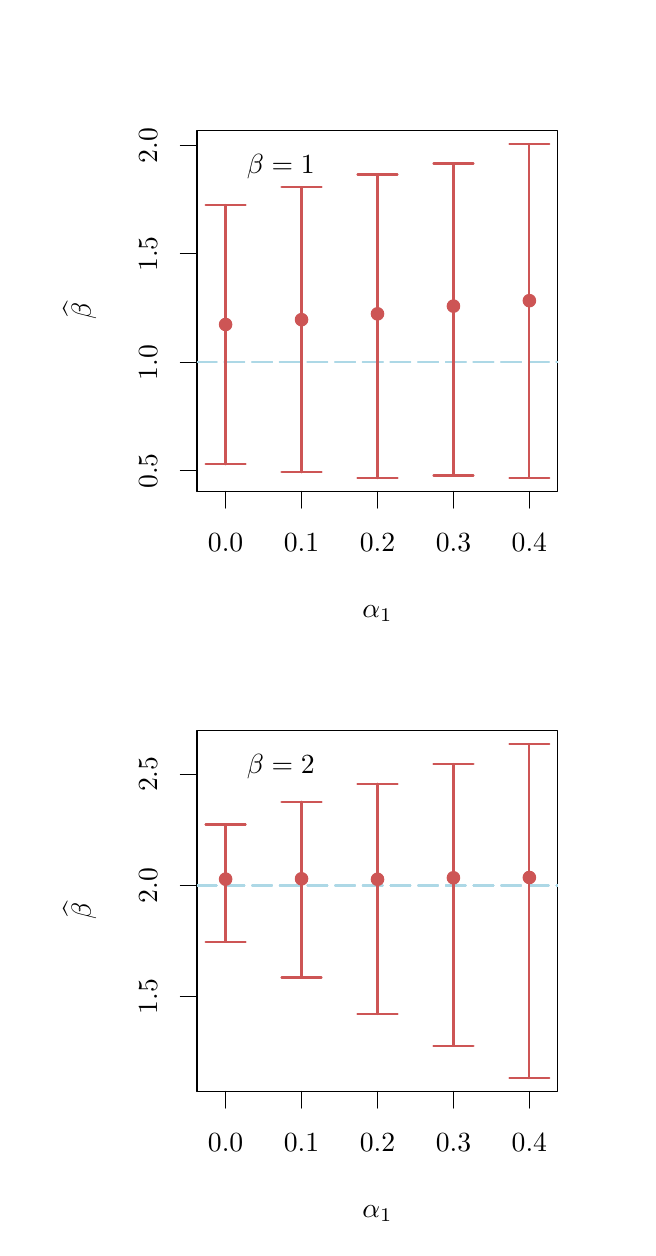
\begin{tikzpicture}[x=1pt,y=1pt]
\definecolor{fillColor}{RGB}{255,255,255}
\path[use as bounding box,fill=fillColor,fill opacity=0.00] (0,0) rectangle (216.81,433.62);
\begin{scope}
\path[clip] ( 61.20,266.01) rectangle (191.61,396.42);
\definecolor{drawColor}{RGB}{255,255,255}
\definecolor{fillColor}{RGB}{255,255,255}

\path[draw=drawColor,line width= 0.4pt,line join=round,line cap=round,fill=fillColor] ( 71.52,326.36) circle (  2.25);

\path[draw=drawColor,line width= 0.4pt,line join=round,line cap=round,fill=fillColor] ( 98.96,328.10) circle (  2.25);

\path[draw=drawColor,line width= 0.4pt,line join=round,line cap=round,fill=fillColor] (126.41,330.21) circle (  2.25);

\path[draw=drawColor,line width= 0.4pt,line join=round,line cap=round,fill=fillColor] (153.85,333.00) circle (  2.25);

\path[draw=drawColor,line width= 0.4pt,line join=round,line cap=round,fill=fillColor] (181.29,334.97) circle (  2.25);
\end{scope}
\begin{scope}
\path[clip] (  0.00,  0.00) rectangle (216.81,433.62);
\definecolor{drawColor}{RGB}{0,0,0}

\path[draw=drawColor,line width= 0.4pt,line join=round,line cap=round] ( 71.52,266.01) -- (181.29,266.01);

\path[draw=drawColor,line width= 0.4pt,line join=round,line cap=round] ( 71.52,266.01) -- ( 71.52,260.01);

\path[draw=drawColor,line width= 0.4pt,line join=round,line cap=round] ( 98.96,266.01) -- ( 98.96,260.01);

\path[draw=drawColor,line width= 0.4pt,line join=round,line cap=round] (126.41,266.01) -- (126.41,260.01);

\path[draw=drawColor,line width= 0.4pt,line join=round,line cap=round] (153.85,266.01) -- (153.85,260.01);

\path[draw=drawColor,line width= 0.4pt,line join=round,line cap=round] (181.29,266.01) -- (181.29,260.01);

\node[text=drawColor,anchor=base,inner sep=0pt, outer sep=0pt, scale=  1.00] at ( 71.52,244.41) {0.0};

\node[text=drawColor,anchor=base,inner sep=0pt, outer sep=0pt, scale=  1.00] at ( 98.96,244.41) {0.1};

\node[text=drawColor,anchor=base,inner sep=0pt, outer sep=0pt, scale=  1.00] at (126.41,244.41) {0.2};

\node[text=drawColor,anchor=base,inner sep=0pt, outer sep=0pt, scale=  1.00] at (153.85,244.41) {0.3};

\node[text=drawColor,anchor=base,inner sep=0pt, outer sep=0pt, scale=  1.00] at (181.29,244.41) {0.4};

\path[draw=drawColor,line width= 0.4pt,line join=round,line cap=round] ( 61.20,273.47) -- ( 61.20,391.09);

\path[draw=drawColor,line width= 0.4pt,line join=round,line cap=round] ( 61.20,273.47) -- ( 55.20,273.47);

\path[draw=drawColor,line width= 0.4pt,line join=round,line cap=round] ( 61.20,312.68) -- ( 55.20,312.68);

\path[draw=drawColor,line width= 0.4pt,line join=round,line cap=round] ( 61.20,351.88) -- ( 55.20,351.88);

\path[draw=drawColor,line width= 0.4pt,line join=round,line cap=round] ( 61.20,391.09) -- ( 55.20,391.09);

\node[text=drawColor,rotate= 90.00,anchor=base,inner sep=0pt, outer sep=0pt, scale=  1.00] at ( 46.80,273.47) {0.5};

\node[text=drawColor,rotate= 90.00,anchor=base,inner sep=0pt, outer sep=0pt, scale=  1.00] at ( 46.80,312.68) {1.0};

\node[text=drawColor,rotate= 90.00,anchor=base,inner sep=0pt, outer sep=0pt, scale=  1.00] at ( 46.80,351.88) {1.5};

\node[text=drawColor,rotate= 90.00,anchor=base,inner sep=0pt, outer sep=0pt, scale=  1.00] at ( 46.80,391.09) {2.0};

\path[draw=drawColor,line width= 0.4pt,line join=round,line cap=round] ( 61.20,266.01) --
	(191.61,266.01) --
	(191.61,396.42) --
	( 61.20,396.42) --
	( 61.20,266.01);
\end{scope}
\begin{scope}
\path[clip] (  0.00,216.81) rectangle (216.81,433.62);
\definecolor{drawColor}{RGB}{0,0,0}

\node[text=drawColor,anchor=base,inner sep=0pt, outer sep=0pt, scale=  1.00] at (126.41,220.41) {$\alpha_1$};

\node[text=drawColor,rotate= 90.00,anchor=base,inner sep=0pt, outer sep=0pt, scale=  1.00] at ( 22.80,331.22) {$\widehat{\beta}$};
\end{scope}
\begin{scope}
\path[clip] ( 61.20,266.01) rectangle (191.61,396.42);
\definecolor{drawColor}{RGB}{0,0,0}

\node[text=drawColor,anchor=base west,inner sep=0pt, outer sep=0pt, scale=  1.00] at ( 79.20,380.98) {$\beta=1$};
\definecolor{drawColor}{RGB}{173,216,230}

\path[draw=drawColor,line width= 0.8pt,dash pattern=on 7pt off 3pt ,line join=round,line cap=round] ( 61.20,312.68) -- (191.61,312.68);

\path[draw=drawColor,line width= 0.8pt,dash pattern=on 7pt off 3pt ,line join=round,line cap=round] ( 61.20,312.68) -- (191.61,312.68);

\path[draw=drawColor,line width= 0.8pt,dash pattern=on 7pt off 3pt ,line join=round,line cap=round] ( 61.20,312.68) -- (191.61,312.68);

\path[draw=drawColor,line width= 0.8pt,dash pattern=on 7pt off 3pt ,line join=round,line cap=round] ( 61.20,312.68) -- (191.61,312.68);

\path[draw=drawColor,line width= 0.8pt,dash pattern=on 7pt off 3pt ,line join=round,line cap=round] ( 61.20,312.68) -- (191.61,312.68);
\definecolor{drawColor}{RGB}{205,85,85}

\path[draw=drawColor,line width= 0.8pt,line join=round,line cap=round] ( 71.52,275.84) -- ( 71.52,369.53);

\path[draw=drawColor,line width= 0.8pt,line join=round,line cap=round] ( 64.29,275.84) --
	( 71.52,275.84) --
	( 78.75,275.84);

\path[draw=drawColor,line width= 0.8pt,line join=round,line cap=round] ( 78.75,369.53) --
	( 71.52,369.53) --
	( 64.29,369.53);

\path[draw=drawColor,line width= 0.8pt,line join=round,line cap=round] ( 98.96,273.00) -- ( 98.96,375.99);

\path[draw=drawColor,line width= 0.8pt,line join=round,line cap=round] ( 91.73,273.00) --
	( 98.96,273.00) --
	(106.19,273.00);

\path[draw=drawColor,line width= 0.8pt,line join=round,line cap=round] (106.19,375.99) --
	( 98.96,375.99) --
	( 91.73,375.99);

\path[draw=drawColor,line width= 0.8pt,line join=round,line cap=round] (126.41,270.84) -- (126.41,380.59);

\path[draw=drawColor,line width= 0.8pt,line join=round,line cap=round] (119.18,270.84) --
	(126.41,270.84) --
	(133.63,270.84);

\path[draw=drawColor,line width= 0.8pt,line join=round,line cap=round] (133.63,380.59) --
	(126.41,380.59) --
	(119.18,380.59);

\path[draw=drawColor,line width= 0.8pt,line join=round,line cap=round] (153.85,271.83) -- (153.85,384.52);

\path[draw=drawColor,line width= 0.8pt,line join=round,line cap=round] (146.62,271.83) --
	(153.85,271.83) --
	(161.08,271.83);

\path[draw=drawColor,line width= 0.8pt,line join=round,line cap=round] (161.08,384.52) --
	(153.85,384.52) --
	(146.62,384.52);

\path[draw=drawColor,line width= 0.8pt,line join=round,line cap=round] (181.29,270.97) -- (181.29,391.59);

\path[draw=drawColor,line width= 0.8pt,line join=round,line cap=round] (174.06,270.97) --
	(181.29,270.97) --
	(188.52,270.97);

\path[draw=drawColor,line width= 0.8pt,line join=round,line cap=round] (188.52,391.59) --
	(181.29,391.59) --
	(174.06,391.59);
\definecolor{fillColor}{RGB}{205,85,85}

\path[draw=drawColor,line width= 0.4pt,line join=round,line cap=round,fill=fillColor] ( 71.52,326.36) circle (  2.25);

\path[draw=drawColor,line width= 0.4pt,line join=round,line cap=round,fill=fillColor] ( 98.96,328.10) circle (  2.25);

\path[draw=drawColor,line width= 0.4pt,line join=round,line cap=round,fill=fillColor] (126.41,330.21) circle (  2.25);

\path[draw=drawColor,line width= 0.4pt,line join=round,line cap=round,fill=fillColor] (153.85,333.00) circle (  2.25);

\path[draw=drawColor,line width= 0.4pt,line join=round,line cap=round,fill=fillColor] (181.29,334.97) circle (  2.25);
\end{scope}
\begin{scope}
\path[clip] ( 61.20, 49.20) rectangle (191.61,179.61);
\definecolor{drawColor}{RGB}{255,255,255}
\definecolor{fillColor}{RGB}{255,255,255}

\path[draw=drawColor,line width= 0.4pt,line join=round,line cap=round,fill=fillColor] ( 71.52,125.94) circle (  2.25);

\path[draw=drawColor,line width= 0.4pt,line join=round,line cap=round,fill=fillColor] ( 98.96,126.06) circle (  2.25);

\path[draw=drawColor,line width= 0.4pt,line join=round,line cap=round,fill=fillColor] (126.41,125.89) circle (  2.25);

\path[draw=drawColor,line width= 0.4pt,line join=round,line cap=round,fill=fillColor] (153.85,126.43) circle (  2.25);

\path[draw=drawColor,line width= 0.4pt,line join=round,line cap=round,fill=fillColor] (181.29,126.54) circle (  2.25);
\end{scope}
\begin{scope}
\path[clip] (  0.00,  0.00) rectangle (216.81,433.62);
\definecolor{drawColor}{RGB}{0,0,0}

\path[draw=drawColor,line width= 0.4pt,line join=round,line cap=round] ( 71.52, 49.20) -- (181.29, 49.20);

\path[draw=drawColor,line width= 0.4pt,line join=round,line cap=round] ( 71.52, 49.20) -- ( 71.52, 43.20);

\path[draw=drawColor,line width= 0.4pt,line join=round,line cap=round] ( 98.96, 49.20) -- ( 98.96, 43.20);

\path[draw=drawColor,line width= 0.4pt,line join=round,line cap=round] (126.41, 49.20) -- (126.41, 43.20);

\path[draw=drawColor,line width= 0.4pt,line join=round,line cap=round] (153.85, 49.20) -- (153.85, 43.20);

\path[draw=drawColor,line width= 0.4pt,line join=round,line cap=round] (181.29, 49.20) -- (181.29, 43.20);

\node[text=drawColor,anchor=base,inner sep=0pt, outer sep=0pt, scale=  1.00] at ( 71.52, 27.60) {0.0};

\node[text=drawColor,anchor=base,inner sep=0pt, outer sep=0pt, scale=  1.00] at ( 98.96, 27.60) {0.1};

\node[text=drawColor,anchor=base,inner sep=0pt, outer sep=0pt, scale=  1.00] at (126.41, 27.60) {0.2};

\node[text=drawColor,anchor=base,inner sep=0pt, outer sep=0pt, scale=  1.00] at (153.85, 27.60) {0.3};

\node[text=drawColor,anchor=base,inner sep=0pt, outer sep=0pt, scale=  1.00] at (181.29, 27.60) {0.4};

\path[draw=drawColor,line width= 0.4pt,line join=round,line cap=round] ( 61.20, 83.50) -- ( 61.20,163.84);

\path[draw=drawColor,line width= 0.4pt,line join=round,line cap=round] ( 61.20, 83.50) -- ( 55.20, 83.50);

\path[draw=drawColor,line width= 0.4pt,line join=round,line cap=round] ( 61.20,123.67) -- ( 55.20,123.67);

\path[draw=drawColor,line width= 0.4pt,line join=round,line cap=round] ( 61.20,163.84) -- ( 55.20,163.84);

\node[text=drawColor,rotate= 90.00,anchor=base,inner sep=0pt, outer sep=0pt, scale=  1.00] at ( 46.80, 83.50) {1.5};

\node[text=drawColor,rotate= 90.00,anchor=base,inner sep=0pt, outer sep=0pt, scale=  1.00] at ( 46.80,123.67) {2.0};

\node[text=drawColor,rotate= 90.00,anchor=base,inner sep=0pt, outer sep=0pt, scale=  1.00] at ( 46.80,163.84) {2.5};

\path[draw=drawColor,line width= 0.4pt,line join=round,line cap=round] ( 61.20, 49.20) --
	(191.61, 49.20) --
	(191.61,179.61) --
	( 61.20,179.61) --
	( 61.20, 49.20);
\end{scope}
\begin{scope}
\path[clip] (  0.00,  0.00) rectangle (216.81,216.81);
\definecolor{drawColor}{RGB}{0,0,0}

\node[text=drawColor,anchor=base,inner sep=0pt, outer sep=0pt, scale=  1.00] at (126.41,  3.60) {$\alpha_1$};

\node[text=drawColor,rotate= 90.00,anchor=base,inner sep=0pt, outer sep=0pt, scale=  1.00] at ( 22.80,114.41) {$\widehat{\beta}$};
\end{scope}
\begin{scope}
\path[clip] ( 61.20, 49.20) rectangle (191.61,179.61);
\definecolor{drawColor}{RGB}{0,0,0}

\node[text=drawColor,anchor=base west,inner sep=0pt, outer sep=0pt, scale=  1.00] at ( 79.20,164.17) {$\beta=2$};
\definecolor{drawColor}{RGB}{173,216,230}

\path[draw=drawColor,line width= 0.8pt,dash pattern=on 7pt off 3pt ,line join=round,line cap=round] ( 61.20,123.67) -- (191.61,123.67);

\path[draw=drawColor,line width= 0.8pt,dash pattern=on 7pt off 3pt ,line join=round,line cap=round] ( 61.20,123.67) -- (191.61,123.67);

\path[draw=drawColor,line width= 0.8pt,dash pattern=on 7pt off 3pt ,line join=round,line cap=round] ( 61.20,123.67) -- (191.61,123.67);

\path[draw=drawColor,line width= 0.8pt,dash pattern=on 7pt off 3pt ,line join=round,line cap=round] ( 61.20,123.67) -- (191.61,123.67);

\path[draw=drawColor,line width= 0.8pt,dash pattern=on 7pt off 3pt ,line join=round,line cap=round] ( 61.20,123.67) -- (191.61,123.67);
\definecolor{drawColor}{RGB}{205,85,85}

\path[draw=drawColor,line width= 0.8pt,line join=round,line cap=round] ( 71.52,103.36) -- ( 71.52,145.69);

\path[draw=drawColor,line width= 0.8pt,line join=round,line cap=round] ( 64.29,103.36) --
	( 71.52,103.36) --
	( 78.75,103.36);

\path[draw=drawColor,line width= 0.8pt,line join=round,line cap=round] ( 78.75,145.69) --
	( 71.52,145.69) --
	( 64.29,145.69);

\path[draw=drawColor,line width= 0.8pt,line join=round,line cap=round] ( 98.96, 90.42) -- ( 98.96,153.91);

\path[draw=drawColor,line width= 0.8pt,line join=round,line cap=round] ( 91.73, 90.42) --
	( 98.96, 90.42) --
	(106.19, 90.42);

\path[draw=drawColor,line width= 0.8pt,line join=round,line cap=round] (106.19,153.91) --
	( 98.96,153.91) --
	( 91.73,153.91);

\path[draw=drawColor,line width= 0.8pt,line join=round,line cap=round] (126.41, 77.19) -- (126.41,160.41);

\path[draw=drawColor,line width= 0.8pt,line join=round,line cap=round] (119.18, 77.19) --
	(126.41, 77.19) --
	(133.63, 77.19);

\path[draw=drawColor,line width= 0.8pt,line join=round,line cap=round] (133.63,160.41) --
	(126.41,160.41) --
	(119.18,160.41);

\path[draw=drawColor,line width= 0.8pt,line join=round,line cap=round] (153.85, 65.69) -- (153.85,167.57);

\path[draw=drawColor,line width= 0.8pt,line join=round,line cap=round] (146.62, 65.69) --
	(153.85, 65.69) --
	(161.08, 65.69);

\path[draw=drawColor,line width= 0.8pt,line join=round,line cap=round] (161.08,167.57) --
	(153.85,167.57) --
	(146.62,167.57);

\path[draw=drawColor,line width= 0.8pt,line join=round,line cap=round] (181.29, 54.03) -- (181.29,174.78);

\path[draw=drawColor,line width= 0.8pt,line join=round,line cap=round] (174.06, 54.03) --
	(181.29, 54.03) --
	(188.52, 54.03);

\path[draw=drawColor,line width= 0.8pt,line join=round,line cap=round] (188.52,174.78) --
	(181.29,174.78) --
	(174.06,174.78);
\definecolor{fillColor}{RGB}{205,85,85}

\path[draw=drawColor,line width= 0.4pt,line join=round,line cap=round,fill=fillColor] ( 71.52,125.94) circle (  2.25);

\path[draw=drawColor,line width= 0.4pt,line join=round,line cap=round,fill=fillColor] ( 98.96,126.06) circle (  2.25);

\path[draw=drawColor,line width= 0.4pt,line join=round,line cap=round,fill=fillColor] (126.41,125.89) circle (  2.25);

\path[draw=drawColor,line width= 0.4pt,line join=round,line cap=round,fill=fillColor] (153.85,126.43) circle (  2.25);

\path[draw=drawColor,line width= 0.4pt,line join=round,line cap=round,fill=fillColor] (181.29,126.54) circle (  2.25);
\end{scope}
\end{tikzpicture}

%  \end{subfigure}
% ~ 
%  \begin{subfigure}[b]{0.31\textwidth}
%\caption{\footnotesize $N=5000, \delta = 0.3$}
%  % Created by tikzDevice version 0.8.1 on 2015-11-17 12:57:40
% !TEX encoding = UTF-8 Unicode
\begin{tikzpicture}[x=1pt,y=1pt]
\definecolor{fillColor}{RGB}{255,255,255}
\path[use as bounding box,fill=fillColor,fill opacity=0.00] (0,0) rectangle (216.81,433.62);
\begin{scope}
\path[clip] (  0.00,  0.00) rectangle (216.81,433.62);
\definecolor{drawColor}{RGB}{0,0,0}

\path[draw=drawColor,line width= 0.4pt,line join=round,line cap=round] ( 71.52,266.01) -- (181.29,266.01);

\path[draw=drawColor,line width= 0.4pt,line join=round,line cap=round] ( 71.52,266.01) -- ( 71.52,260.01);

\path[draw=drawColor,line width= 0.4pt,line join=round,line cap=round] ( 98.96,266.01) -- ( 98.96,260.01);

\path[draw=drawColor,line width= 0.4pt,line join=round,line cap=round] (126.41,266.01) -- (126.41,260.01);

\path[draw=drawColor,line width= 0.4pt,line join=round,line cap=round] (153.85,266.01) -- (153.85,260.01);

\path[draw=drawColor,line width= 0.4pt,line join=round,line cap=round] (181.29,266.01) -- (181.29,260.01);

\node[text=drawColor,anchor=base,inner sep=0pt, outer sep=0pt, scale=  1.00] at ( 71.52,244.41) {0.0};

\node[text=drawColor,anchor=base,inner sep=0pt, outer sep=0pt, scale=  1.00] at ( 98.96,244.41) {0.1};

\node[text=drawColor,anchor=base,inner sep=0pt, outer sep=0pt, scale=  1.00] at (126.41,244.41) {0.2};

\node[text=drawColor,anchor=base,inner sep=0pt, outer sep=0pt, scale=  1.00] at (153.85,244.41) {0.3};

\node[text=drawColor,anchor=base,inner sep=0pt, outer sep=0pt, scale=  1.00] at (181.29,244.41) {0.4};

\path[draw=drawColor,line width= 0.4pt,line join=round,line cap=round] ( 61.20,266.01) --
	(191.61,266.01) --
	(191.61,396.42) --
	( 61.20,396.42) --
	( 61.20,266.01);
\end{scope}
\begin{scope}
\path[clip] (  0.00,216.81) rectangle (216.81,433.62);
\definecolor{drawColor}{RGB}{0,0,0}

\node[text=drawColor,anchor=base,inner sep=0pt, outer sep=0pt, scale=  1.00] at (126.41,220.41) {$\alpha_1$};

\node[text=drawColor,rotate= 90.00,anchor=base,inner sep=0pt, outer sep=0pt, scale=  1.00] at ( 22.80,331.22) {$\widehat{\beta}$};
\end{scope}
\begin{scope}
\path[clip] (  0.00,  0.00) rectangle (216.81,433.62);
\definecolor{drawColor}{RGB}{0,0,0}

\path[draw=drawColor,line width= 0.4pt,line join=round,line cap=round] ( 61.20,270.84) -- ( 61.20,391.59);

\path[draw=drawColor,line width= 0.4pt,line join=round,line cap=round] ( 61.20,270.84) -- ( 55.20,270.84);

\path[draw=drawColor,line width= 0.4pt,line join=round,line cap=round] ( 61.20,301.03) -- ( 55.20,301.03);

\path[draw=drawColor,line width= 0.4pt,line join=round,line cap=round] ( 61.20,331.22) -- ( 55.20,331.22);

\path[draw=drawColor,line width= 0.4pt,line join=round,line cap=round] ( 61.20,361.40) -- ( 55.20,361.40);

\path[draw=drawColor,line width= 0.4pt,line join=round,line cap=round] ( 61.20,391.59) -- ( 55.20,391.59);

\node[text=drawColor,rotate= 90.00,anchor=base,inner sep=0pt, outer sep=0pt, scale=  1.00] at ( 46.80,270.84) {0};

\node[text=drawColor,rotate= 90.00,anchor=base,inner sep=0pt, outer sep=0pt, scale=  1.00] at ( 46.80,331.22) {1};

\node[text=drawColor,rotate= 90.00,anchor=base,inner sep=0pt, outer sep=0pt, scale=  1.00] at ( 46.80,391.59) {2};
\end{scope}
\begin{scope}
\path[clip] ( 61.20,266.01) rectangle (191.61,396.42);
\definecolor{drawColor}{RGB}{0,0,0}

\node[text=drawColor,anchor=base west,inner sep=0pt, outer sep=0pt, scale=  1.00] at ( 79.20,380.98) {$\beta=1$};
\definecolor{drawColor}{RGB}{173,216,230}

\path[draw=drawColor,line width= 0.8pt,dash pattern=on 7pt off 3pt ,line join=round,line cap=round] ( 61.20,331.22) -- (191.61,331.22);

\path[draw=drawColor,line width= 0.8pt,dash pattern=on 7pt off 3pt ,line join=round,line cap=round] ( 61.20,331.22) -- (191.61,331.22);

\path[draw=drawColor,line width= 0.8pt,dash pattern=on 7pt off 3pt ,line join=round,line cap=round] ( 61.20,331.22) -- (191.61,331.22);

\path[draw=drawColor,line width= 0.8pt,dash pattern=on 7pt off 3pt ,line join=round,line cap=round] ( 61.20,331.22) -- (191.61,331.22);

\path[draw=drawColor,line width= 0.8pt,dash pattern=on 7pt off 3pt ,line join=round,line cap=round] ( 61.20,331.22) -- (191.61,331.22);
\definecolor{drawColor}{RGB}{205,85,85}

\path[draw=drawColor,line width= 0.8pt,line join=round,line cap=round] ( 71.52,312.28) -- ( 71.52,348.61);

\path[draw=drawColor,line width= 0.8pt,line join=round,line cap=round] ( 64.29,312.28) --
	( 71.52,312.28) --
	( 78.75,312.28);

\path[draw=drawColor,line width= 0.8pt,line join=round,line cap=round] ( 78.75,348.61) --
	( 71.52,348.61) --
	( 64.29,348.61);

\path[draw=drawColor,line width= 0.8pt,line join=round,line cap=round] ( 98.96,308.63) -- ( 98.96,350.58);

\path[draw=drawColor,line width= 0.8pt,line join=round,line cap=round] ( 91.73,308.63) --
	( 98.96,308.63) --
	(106.19,308.63);

\path[draw=drawColor,line width= 0.8pt,line join=round,line cap=round] (106.19,350.58) --
	( 98.96,350.58) --
	( 91.73,350.58);

\path[draw=drawColor,line width= 0.8pt,line join=round,line cap=round] (126.41,305.11) -- (126.41,353.12);

\path[draw=drawColor,line width= 0.8pt,line join=round,line cap=round] (119.18,305.11) --
	(126.41,305.11) --
	(133.63,305.11);

\path[draw=drawColor,line width= 0.8pt,line join=round,line cap=round] (133.63,353.12) --
	(126.41,353.12) --
	(119.18,353.12);

\path[draw=drawColor,line width= 0.8pt,line join=round,line cap=round] (153.85,302.04) -- (153.85,355.16);

\path[draw=drawColor,line width= 0.8pt,line join=round,line cap=round] (146.62,302.04) --
	(153.85,302.04) --
	(161.08,302.04);

\path[draw=drawColor,line width= 0.8pt,line join=round,line cap=round] (161.08,355.16) --
	(153.85,355.16) --
	(146.62,355.16);

\path[draw=drawColor,line width= 0.8pt,line join=round,line cap=round] (181.29,299.66) -- (181.29,358.75);

\path[draw=drawColor,line width= 0.8pt,line join=round,line cap=round] (174.06,299.66) --
	(181.29,299.66) --
	(188.52,299.66);

\path[draw=drawColor,line width= 0.8pt,line join=round,line cap=round] (188.52,358.75) --
	(181.29,358.75) --
	(174.06,358.75);
\definecolor{fillColor}{RGB}{205,85,85}

\path[draw=drawColor,line width= 0.4pt,line join=round,line cap=round,fill=fillColor] ( 71.52,333.19) circle (  2.25);

\path[draw=drawColor,line width= 0.4pt,line join=round,line cap=round,fill=fillColor] ( 98.96,333.20) circle (  2.25);

\path[draw=drawColor,line width= 0.4pt,line join=round,line cap=round,fill=fillColor] (126.41,333.33) circle (  2.25);

\path[draw=drawColor,line width= 0.4pt,line join=round,line cap=round,fill=fillColor] (153.85,333.68) circle (  2.25);

\path[draw=drawColor,line width= 0.4pt,line join=round,line cap=round,fill=fillColor] (181.29,334.38) circle (  2.25);
\end{scope}
\begin{scope}
\path[clip] (  0.00,  0.00) rectangle (216.81,433.62);
\definecolor{drawColor}{RGB}{0,0,0}

\path[draw=drawColor,line width= 0.4pt,line join=round,line cap=round] ( 71.52, 49.20) -- (181.29, 49.20);

\path[draw=drawColor,line width= 0.4pt,line join=round,line cap=round] ( 71.52, 49.20) -- ( 71.52, 43.20);

\path[draw=drawColor,line width= 0.4pt,line join=round,line cap=round] ( 98.96, 49.20) -- ( 98.96, 43.20);

\path[draw=drawColor,line width= 0.4pt,line join=round,line cap=round] (126.41, 49.20) -- (126.41, 43.20);

\path[draw=drawColor,line width= 0.4pt,line join=round,line cap=round] (153.85, 49.20) -- (153.85, 43.20);

\path[draw=drawColor,line width= 0.4pt,line join=round,line cap=round] (181.29, 49.20) -- (181.29, 43.20);

\node[text=drawColor,anchor=base,inner sep=0pt, outer sep=0pt, scale=  1.00] at ( 71.52, 27.60) {0.0};

\node[text=drawColor,anchor=base,inner sep=0pt, outer sep=0pt, scale=  1.00] at ( 98.96, 27.60) {0.1};

\node[text=drawColor,anchor=base,inner sep=0pt, outer sep=0pt, scale=  1.00] at (126.41, 27.60) {0.2};

\node[text=drawColor,anchor=base,inner sep=0pt, outer sep=0pt, scale=  1.00] at (153.85, 27.60) {0.3};

\node[text=drawColor,anchor=base,inner sep=0pt, outer sep=0pt, scale=  1.00] at (181.29, 27.60) {0.4};

\path[draw=drawColor,line width= 0.4pt,line join=round,line cap=round] ( 61.20, 49.20) --
	(191.61, 49.20) --
	(191.61,179.61) --
	( 61.20,179.61) --
	( 61.20, 49.20);
\end{scope}
\begin{scope}
\path[clip] (  0.00,  0.00) rectangle (216.81,216.81);
\definecolor{drawColor}{RGB}{0,0,0}

\node[text=drawColor,anchor=base,inner sep=0pt, outer sep=0pt, scale=  1.00] at (126.41,  3.60) {$\alpha_1$};

\node[text=drawColor,rotate= 90.00,anchor=base,inner sep=0pt, outer sep=0pt, scale=  1.00] at ( 22.80,114.41) {$\widehat{\beta}$};
\end{scope}
\begin{scope}
\path[clip] (  0.00,  0.00) rectangle (216.81,433.62);
\definecolor{drawColor}{RGB}{0,0,0}

\path[draw=drawColor,line width= 0.4pt,line join=round,line cap=round] ( 61.20, 54.03) -- ( 61.20,174.78);

\path[draw=drawColor,line width= 0.4pt,line join=round,line cap=round] ( 61.20, 54.03) -- ( 55.20, 54.03);

\path[draw=drawColor,line width= 0.4pt,line join=round,line cap=round] ( 61.20, 84.22) -- ( 55.20, 84.22);

\path[draw=drawColor,line width= 0.4pt,line join=round,line cap=round] ( 61.20,114.41) -- ( 55.20,114.41);

\path[draw=drawColor,line width= 0.4pt,line join=round,line cap=round] ( 61.20,144.59) -- ( 55.20,144.59);

\path[draw=drawColor,line width= 0.4pt,line join=round,line cap=round] ( 61.20,174.78) -- ( 55.20,174.78);

\node[text=drawColor,rotate= 90.00,anchor=base,inner sep=0pt, outer sep=0pt, scale=  1.00] at ( 46.80, 54.03) {1};

\node[text=drawColor,rotate= 90.00,anchor=base,inner sep=0pt, outer sep=0pt, scale=  1.00] at ( 46.80,114.41) {2};

\node[text=drawColor,rotate= 90.00,anchor=base,inner sep=0pt, outer sep=0pt, scale=  1.00] at ( 46.80,174.78) {3};
\end{scope}
\begin{scope}
\path[clip] ( 61.20, 49.20) rectangle (191.61,179.61);
\definecolor{drawColor}{RGB}{0,0,0}

\node[text=drawColor,anchor=base west,inner sep=0pt, outer sep=0pt, scale=  1.00] at ( 79.20,164.17) {$\beta=2$};
\definecolor{drawColor}{RGB}{173,216,230}

\path[draw=drawColor,line width= 0.8pt,dash pattern=on 7pt off 3pt ,line join=round,line cap=round] ( 61.20,114.41) -- (191.61,114.41);

\path[draw=drawColor,line width= 0.8pt,dash pattern=on 7pt off 3pt ,line join=round,line cap=round] ( 61.20,114.41) -- (191.61,114.41);

\path[draw=drawColor,line width= 0.8pt,dash pattern=on 7pt off 3pt ,line join=round,line cap=round] ( 61.20,114.41) -- (191.61,114.41);

\path[draw=drawColor,line width= 0.8pt,dash pattern=on 7pt off 3pt ,line join=round,line cap=round] ( 61.20,114.41) -- (191.61,114.41);

\path[draw=drawColor,line width= 0.8pt,dash pattern=on 7pt off 3pt ,line join=round,line cap=round] ( 61.20,114.41) -- (191.61,114.41);
\definecolor{drawColor}{RGB}{205,85,85}

\path[draw=drawColor,line width= 0.8pt,line join=round,line cap=round] ( 71.52,107.31) -- ( 71.52,121.73);

\path[draw=drawColor,line width= 0.8pt,line join=round,line cap=round] ( 64.29,107.31) --
	( 71.52,107.31) --
	( 78.75,107.31);

\path[draw=drawColor,line width= 0.8pt,line join=round,line cap=round] ( 78.75,121.73) --
	( 71.52,121.73) --
	( 64.29,121.73);

\path[draw=drawColor,line width= 0.8pt,line join=round,line cap=round] ( 98.96,103.84) -- ( 98.96,124.43);

\path[draw=drawColor,line width= 0.8pt,line join=round,line cap=round] ( 91.73,103.84) --
	( 98.96,103.84) --
	(106.19,103.84);

\path[draw=drawColor,line width= 0.8pt,line join=round,line cap=round] (106.19,124.43) --
	( 98.96,124.43) --
	( 91.73,124.43);

\path[draw=drawColor,line width= 0.8pt,line join=round,line cap=round] (126.41,100.67) -- (126.41,127.03);

\path[draw=drawColor,line width= 0.8pt,line join=round,line cap=round] (119.18,100.67) --
	(126.41,100.67) --
	(133.63,100.67);

\path[draw=drawColor,line width= 0.8pt,line join=round,line cap=round] (133.63,127.03) --
	(126.41,127.03) --
	(119.18,127.03);

\path[draw=drawColor,line width= 0.8pt,line join=round,line cap=round] (153.85, 97.08) -- (153.85,129.82);

\path[draw=drawColor,line width= 0.8pt,line join=round,line cap=round] (146.62, 97.08) --
	(153.85, 97.08) --
	(161.08, 97.08);

\path[draw=drawColor,line width= 0.8pt,line join=round,line cap=round] (161.08,129.82) --
	(153.85,129.82) --
	(146.62,129.82);

\path[draw=drawColor,line width= 0.8pt,line join=round,line cap=round] (181.29, 92.67) -- (181.29,132.56);

\path[draw=drawColor,line width= 0.8pt,line join=round,line cap=round] (174.06, 92.67) --
	(181.29, 92.67) --
	(188.52, 92.67);

\path[draw=drawColor,line width= 0.8pt,line join=round,line cap=round] (188.52,132.56) --
	(181.29,132.56) --
	(174.06,132.56);
\definecolor{fillColor}{RGB}{205,85,85}

\path[draw=drawColor,line width= 0.4pt,line join=round,line cap=round,fill=fillColor] ( 71.52,114.79) circle (  2.25);

\path[draw=drawColor,line width= 0.4pt,line join=round,line cap=round,fill=fillColor] ( 98.96,114.74) circle (  2.25);

\path[draw=drawColor,line width= 0.4pt,line join=round,line cap=round,fill=fillColor] (126.41,114.70) circle (  2.25);

\path[draw=drawColor,line width= 0.4pt,line join=round,line cap=round,fill=fillColor] (153.85,114.82) circle (  2.25);

\path[draw=drawColor,line width= 0.4pt,line join=round,line cap=round,fill=fillColor] (181.29,114.78) circle (  2.25);
\end{scope}
\end{tikzpicture}

%  \end{subfigure}
%\endgroup
%\end{figure}
%\end{frame}
%%%%%%%%%%%%%%%%%%%%%%%%%%%%%%%%%%%%%
\end{document}
